\documentclass[]{book}
\usepackage{lmodern}
\usepackage{amssymb,amsmath}
\usepackage{ifxetex,ifluatex}
\usepackage{fixltx2e} % provides \textsubscript
\ifnum 0\ifxetex 1\fi\ifluatex 1\fi=0 % if pdftex
  \usepackage[T1]{fontenc}
  \usepackage[utf8]{inputenc}
\else % if luatex or xelatex
  \ifxetex
    \usepackage{mathspec}
  \else
    \usepackage{fontspec}
  \fi
  \defaultfontfeatures{Ligatures=TeX,Scale=MatchLowercase}
\fi
% use upquote if available, for straight quotes in verbatim environments
\IfFileExists{upquote.sty}{\usepackage{upquote}}{}
% use microtype if available
\IfFileExists{microtype.sty}{%
\usepackage{microtype}
\UseMicrotypeSet[protrusion]{basicmath} % disable protrusion for tt fonts
}{}
\usepackage[margin=1in]{geometry}
\usepackage{hyperref}
\PassOptionsToPackage{usenames,dvipsnames}{color} % color is loaded by hyperref
\hypersetup{unicode=true,
            pdftitle={Introduction to R for Natural Resource Scientists},
            pdfauthor={Ben Staton},
            colorlinks=true,
            linkcolor=blue,
            citecolor=Blue,
            urlcolor=blue,
            breaklinks=true}
\urlstyle{same}  % don't use monospace font for urls
\usepackage{natbib}
\bibliographystyle{apalike}
\usepackage{color}
\usepackage{fancyvrb}
\newcommand{\VerbBar}{|}
\newcommand{\VERB}{\Verb[commandchars=\\\{\}]}
\DefineVerbatimEnvironment{Highlighting}{Verbatim}{commandchars=\\\{\}}
% Add ',fontsize=\small' for more characters per line
\usepackage{framed}
\definecolor{shadecolor}{RGB}{248,248,248}
\newenvironment{Shaded}{\begin{snugshade}}{\end{snugshade}}
\newcommand{\KeywordTok}[1]{\textcolor[rgb]{0.13,0.29,0.53}{\textbf{#1}}}
\newcommand{\DataTypeTok}[1]{\textcolor[rgb]{0.13,0.29,0.53}{#1}}
\newcommand{\DecValTok}[1]{\textcolor[rgb]{0.00,0.00,0.81}{#1}}
\newcommand{\BaseNTok}[1]{\textcolor[rgb]{0.00,0.00,0.81}{#1}}
\newcommand{\FloatTok}[1]{\textcolor[rgb]{0.00,0.00,0.81}{#1}}
\newcommand{\ConstantTok}[1]{\textcolor[rgb]{0.00,0.00,0.00}{#1}}
\newcommand{\CharTok}[1]{\textcolor[rgb]{0.31,0.60,0.02}{#1}}
\newcommand{\SpecialCharTok}[1]{\textcolor[rgb]{0.00,0.00,0.00}{#1}}
\newcommand{\StringTok}[1]{\textcolor[rgb]{0.31,0.60,0.02}{#1}}
\newcommand{\VerbatimStringTok}[1]{\textcolor[rgb]{0.31,0.60,0.02}{#1}}
\newcommand{\SpecialStringTok}[1]{\textcolor[rgb]{0.31,0.60,0.02}{#1}}
\newcommand{\ImportTok}[1]{#1}
\newcommand{\CommentTok}[1]{\textcolor[rgb]{0.56,0.35,0.01}{\textit{#1}}}
\newcommand{\DocumentationTok}[1]{\textcolor[rgb]{0.56,0.35,0.01}{\textbf{\textit{#1}}}}
\newcommand{\AnnotationTok}[1]{\textcolor[rgb]{0.56,0.35,0.01}{\textbf{\textit{#1}}}}
\newcommand{\CommentVarTok}[1]{\textcolor[rgb]{0.56,0.35,0.01}{\textbf{\textit{#1}}}}
\newcommand{\OtherTok}[1]{\textcolor[rgb]{0.56,0.35,0.01}{#1}}
\newcommand{\FunctionTok}[1]{\textcolor[rgb]{0.00,0.00,0.00}{#1}}
\newcommand{\VariableTok}[1]{\textcolor[rgb]{0.00,0.00,0.00}{#1}}
\newcommand{\ControlFlowTok}[1]{\textcolor[rgb]{0.13,0.29,0.53}{\textbf{#1}}}
\newcommand{\OperatorTok}[1]{\textcolor[rgb]{0.81,0.36,0.00}{\textbf{#1}}}
\newcommand{\BuiltInTok}[1]{#1}
\newcommand{\ExtensionTok}[1]{#1}
\newcommand{\PreprocessorTok}[1]{\textcolor[rgb]{0.56,0.35,0.01}{\textit{#1}}}
\newcommand{\AttributeTok}[1]{\textcolor[rgb]{0.77,0.63,0.00}{#1}}
\newcommand{\RegionMarkerTok}[1]{#1}
\newcommand{\InformationTok}[1]{\textcolor[rgb]{0.56,0.35,0.01}{\textbf{\textit{#1}}}}
\newcommand{\WarningTok}[1]{\textcolor[rgb]{0.56,0.35,0.01}{\textbf{\textit{#1}}}}
\newcommand{\AlertTok}[1]{\textcolor[rgb]{0.94,0.16,0.16}{#1}}
\newcommand{\ErrorTok}[1]{\textcolor[rgb]{0.64,0.00,0.00}{\textbf{#1}}}
\newcommand{\NormalTok}[1]{#1}
\usepackage{longtable,booktabs}
\usepackage{graphicx,grffile}
\makeatletter
\def\maxwidth{\ifdim\Gin@nat@width>\linewidth\linewidth\else\Gin@nat@width\fi}
\def\maxheight{\ifdim\Gin@nat@height>\textheight\textheight\else\Gin@nat@height\fi}
\makeatother
% Scale images if necessary, so that they will not overflow the page
% margins by default, and it is still possible to overwrite the defaults
% using explicit options in \includegraphics[width, height, ...]{}
\setkeys{Gin}{width=\maxwidth,height=\maxheight,keepaspectratio}
\IfFileExists{parskip.sty}{%
\usepackage{parskip}
}{% else
\setlength{\parindent}{0pt}
\setlength{\parskip}{6pt plus 2pt minus 1pt}
}
\setlength{\emergencystretch}{3em}  % prevent overfull lines
\providecommand{\tightlist}{%
  \setlength{\itemsep}{0pt}\setlength{\parskip}{0pt}}
\setcounter{secnumdepth}{5}
% Redefines (sub)paragraphs to behave more like sections
\ifx\paragraph\undefined\else
\let\oldparagraph\paragraph
\renewcommand{\paragraph}[1]{\oldparagraph{#1}\mbox{}}
\fi
\ifx\subparagraph\undefined\else
\let\oldsubparagraph\subparagraph
\renewcommand{\subparagraph}[1]{\oldsubparagraph{#1}\mbox{}}
\fi

%%% Use protect on footnotes to avoid problems with footnotes in titles
\let\rmarkdownfootnote\footnote%
\def\footnote{\protect\rmarkdownfootnote}

%%% Change title format to be more compact
\usepackage{titling}

% Create subtitle command for use in maketitle
\newcommand{\subtitle}[1]{
  \posttitle{
    \begin{center}\large#1\end{center}
    }
}

\setlength{\droptitle}{-2em}

  \title{Introduction to R for Natural Resource Scientists}
    \pretitle{\vspace{\droptitle}\centering\huge}
  \posttitle{\par}
    \author{Ben Staton}
    \preauthor{\centering\large\emph}
  \postauthor{\par}
      \predate{\centering\large\emph}
  \postdate{\par}
    \date{with contributions from Henry Hershey}

\usepackage{booktabs}
\usepackage{pdfpages}
\usepackage{amsthm}
\makeatletter
\def\thm@space@setup{%
  \thm@preskip=8pt plus 2pt minus 4pt
  \thm@postskip=\thm@preskip
}
\makeatother
\let\oldmaketitle\maketitle
\AtBeginDocument{\let\maketitle\relax}
\usepackage{booktabs}
\usepackage{longtable}
\usepackage{array}
\usepackage{multirow}
\usepackage[table]{xcolor}
\usepackage{wrapfig}
\usepackage{float}
\usepackage{colortbl}
\usepackage{pdflscape}
\usepackage{tabu}
\usepackage{threeparttable}
\usepackage{threeparttablex}
\usepackage[normalem]{ulem}
\usepackage{makecell}

\usepackage{amsthm}
\newtheorem{theorem}{Theorem}[chapter]
\newtheorem{lemma}{Lemma}[chapter]
\theoremstyle{definition}
\newtheorem{definition}{Definition}[chapter]
\newtheorem{corollary}{Corollary}[chapter]
\newtheorem{proposition}{Proposition}[chapter]
\theoremstyle{definition}
\newtheorem{example}{Example}[chapter]
\theoremstyle{definition}
\newtheorem{exercise}{Exercise}[chapter]
\theoremstyle{remark}
\newtheorem*{remark}{Remark}
\newtheorem*{solution}{Solution}
\begin{document}
\maketitle

% % \thispagestyle{empty}
% \begin{center}
% % {\Huge A BOOK}
% 
\includegraphics{cover_image.png}
% % {\huge by Me}
% \end{center}
% 
% \let\maketitle\oldmaketitle
% \maketitle

% \cleardoublepage\newpage\thispagestyle{empty}\null
% \cleardoublepage\newpage\thispagestyle{empty}\null
% \cleardoublepage\newpage
% \thispagestyle{empty}
% \cleardoublepage\begin{center}
% \newgeometry{left=0cm,right=0cm,top=0cm,bottom=0cm}
% 
\includegraphics{cover_image.png}
% \restoregeometry
% \end{center}
% \setlength{\abovedisplayskip}{-5pt}
% \setlength{\abovedisplayshortskip}{-5pt}


\includepdf[pages={1}]{Cover_Page.pdf}
\thispagestyle{empty}
\let\maketitle\oldmaketitle
\maketitle
\thispagestyle{empty}

{
\hypersetup{linkcolor=black}
\setcounter{tocdepth}{1}
\tableofcontents
}
\chapter*{Overview}\label{overview}
\addcontentsline{toc}{chapter}{Overview}

This book is intended to be a first course in R programming for natural
resource professionals. It is by no means comprehensive (no book about R
ever could be), but instead attempts to introduce the main topics needed
to get a beginner up and running with applying R to their own work. It
is intended to be a companion to in-person workshop sessions, in which
each chapter is covered in a 2 hour session, however it can be used as
``self-teach'' manual as well. Although the examples shown have a
natural resource/ecological theme, the general skills presented are
general to R users across all scientific disciplines.

\section*{What is Covered?}\label{what-is-covered}
\addcontentsline{toc}{section}{What is Covered?}

The book is composed of six chapters intended to cover a suite of topics
in introductory R programming. In general, the material builds in
complexity from chapter to chapter and earlier chapters can be seen as
prerequisites for later chapters.

\begin{itemize}
\tightlist
\item
  \textbf{Chapter \ref{ch1}} covers the basics of working in R through
  RStudio, including the basics of the R coding language and
  environment.
\item
  \textbf{Chapter \ref{ch2}} covers the basics of plotting using the
  base R graphics functionality.
\item
  \textbf{Chapter \ref{ch3}} covers the basics of fitting statistical
  models using built-in functionality for generalized linear models as
  well as non-linear models.\\
\item
  \textbf{Chapter \ref{ch4}} covers the basics of simulation modeling in
  R.
\item
  \textbf{Chapter \ref{ch5}} covers the basics of the \texttt{\{dplyr\}}
  and \texttt{\{reshape2\}} packages for manipulating and summarizing
  large data sets using highly readable code.
\item
  \textbf{Chapter \ref{ch6}} covers the basics of producing maps and
  performing spatial analysis in R. \emph{This chapter was contributed
  by Henry Hershey}
\end{itemize}

\section*{Prerequisites}\label{prerequisites}
\addcontentsline{toc}{section}{Prerequisites}

Chapter \ref{ch1} starts at the first step (installing R) and progresses
by assuming no prior knowledge of programming in R or in any other
language. In the later chapters, e.g., Chapters \ref{ch3} and \ref{ch4},
an understanding of statistics at the introductory undergraduate level
would be helpful but not strictly essential.

There are, however, some tasks you'll need to complete before using this
book, which are described in the two sections that follow.

\subsection*{Prepare Your Computer}\label{comp-prep}
\addcontentsline{toc}{subsection}{Prepare Your Computer}

You will install R and RStudio as the first step in Chapter 1. See
\protect\hyperlink{install}{here} for the links to get these programs.

You should create a devoted folder on your computer for this book. All
examples will assume this folder is located here:
\texttt{C:/Users/YOU/Documents/R-Book}.

Change \texttt{YOU} to be specific for your computer.

\hypertarget{data-sets}{\subsection*{Data Sets}\label{data-sets}}
\addcontentsline{toc}{subsection}{Data Sets}

The data sets\footnote{Many of the data sets used in this book were
  simulated by the author. Cases in which the data set used was not
  simulated are noted and a citation to the data source is provided.
  More details on the individual data sets can be found on the GitHub
  repository.} used in this book are hosted on a GitHub repository
maintained by the author. It is located here:
\url{https://github.com/bstaton1/au-r-workshop-data}.

To acquire the data for this book, you should:

\begin{enumerate}
\def\labelenumi{\arabic{enumi}.}
\tightlist
\item
  Navigate to the GitHub repository
\item
  click the green \emph{Clone or download} button at the top right,
\item
  click \emph{Download ZIP}
\item
  unzip the contents of this folder into the location:
  \texttt{C:/Users/YOU/Documents/R-Book/Data}
\end{enumerate}

\section*{Exercises}\label{exercises}
\addcontentsline{toc}{section}{Exercises}

Following each chapter, there is a set of exercises. You should attempt
and complete them, as they give you an opportunity to practice what you
learned while reading and typing along. Solutions are provided at the
end of this book, however you are \textbf{strongly} recommended to
attempt to figure the problems out on your own before looking to how the
author would solve them.

Some exercises have bonus questions. These are intended to challenge you
with some of the more difficult tasks shown in the chapter or ask you to
extend what you learned to a completely different problem. If you can
get all of the non-bonus questions without looking at the solutions too
much, you can consider yourself to have good understanding of that
chapter's material. If you can complete the bonus questions with little
or no help, that means you have mastered that chapter's material!

\hypertarget{notation}{\section*{Text Conventions}\label{notation}}
\addcontentsline{toc}{section}{Text Conventions}

\begin{itemize}
\tightlist
\item
  Regular text: a description of what you you should do, how some code
  works, or a general narrative of something.
\item
  \texttt{monospace}: references something in R

  \begin{itemize}
  \tightlist
  \item
    \texttt{this()} references some function
  \item
    \texttt{this} references some other object
  \item
    \texttt{\{this\}} references an R package
  \item
    \texttt{C:/This} is a file path
  \end{itemize}
\item
  \textbf{Bold} is intended to provide more emphasis to a word or topic.
  In general, new topics are introduced this way.
\item
  \protect\hyperlink{notation}{Links}: this is a link to some other
  location in this book. External links are provided with a full URL.
\item
  \(Equations\): it is sometimes useful to describe concepts
  mathematically before showing how to do it in R.
\item
  \footnote{This is a footnote}: a footnote containing more information.
\end{itemize}

\section*{Keyboard Shortcuts}\label{keyboard-shortcuts}
\addcontentsline{toc}{section}{Keyboard Shortcuts}

Several parts of this book in this book make reference to keyboard
shortcuts. They are never necessary, but can help you be more efficient
if you commit them to muscle memory. This book assumes you are using a
PC for the keyboard shortcuts. If you are using a Mac, they will be
different\footnote{For some keyboard shortcuts, you may just need to
  swap out the \textbf{CTRL} keystroke for the \textbf{CMD} keystroke
  for a Mac computer}. For a complete list of RStudio's keyboard
shortcuts specific to your operating system, go to \emph{Help
\textgreater{} Keyboard Shortcuts Help}.

\section*{Development of this Book}\label{development-of-this-book}
\addcontentsline{toc}{section}{Development of this Book}

This book represents the third reincarnation of the Auburn R Workshop
Series. The first version was written in Fall 2014 using Microsoft Word,
but the author found that making even small changes was clunky - each
change to code in the document required a copy-paste of code and output
from R to Word. Individual session materials (i.e., handout, exercises,
solutions, data) were created in separate documents, saved as pdfs and
\texttt{.xlsx} files, and uploaded to a wordpress webpage.

The second version was written through R and RStudio using the R
packages \texttt{\{rmarkdown\}} \citep{rmarkdown-cite} and
\texttt{\{knitr\}} \citep{knitr-cite}, which allowed the integration of
text, code, and output all into one output file. This version was
completed in Fall 2015. Like the first version, individual session
materials were created in separate documents, and replaced those
previously found on the wordpress site.

This third version was written through R and RStudio but used the R
package \texttt{\{bookdown\}} \citep{bookdown-cite} which allowed for
the individual sessions to be combined into one ``book'' by turning each
session into a chapter. This facilitated cross-references to topics
covered in previous chapters and allows the reader to only refer to one
location when trying to remember how to use a skill. It also allowed for
multiple formats to be published including both HTML and PDF versions.

The book is hosted on \href{https://pages.github.com/}{GitHub Pages},
and was last built on 09-25-2018.

\section*{About the Author}\label{about-the-author}
\addcontentsline{toc}{section}{About the Author}

Ben Staton is a PhD candidate in the School of Fisheries at Auburn
University. He studies quantitative methods for assessing fish
populations for use in harvest management, with a focus on Pacific
salmon in western Alaska. His interests are in population dynamics,
Bayesian methods, Monte Carlo methods, and reproducible research. Ben
has been using R on a daily basis since the beginning of his graduate
work in 2014, and is enthusiastic about helping others learn to use R
for their own work.

\chapter{Introduction to the R Environment}\label{ch1}

\section*{Chapter Overview}\label{chapter-overview}
\addcontentsline{toc}{section}{Chapter Overview}

In this first chapter, you will get familiar with the basics of using R.
You will learn:

\begin{itemize}
\tightlist
\item
  how to use R as a basic calculator
\item
  some basic object types
\item
  some basic data classes
\item
  some basic data structures
\item
  how to read in data
\item
  how to produce basic data summaries
\item
  how to write out data
\item
  how to write your own functions
\end{itemize}

\section*{Before You Begin: Install R and
RStudio}\label{before-you-begin-install-r-and-rstudio}
\addcontentsline{toc}{section}{Before You Begin: Install R and RStudio}

First off, you will need to get R and RStudio\footnote{While it is
  possible to run R on its own, it is clunky. You are strongly advised
  to use the RStudio IDE (integrated development environment) given its
  compactness, neat features, code tools (like syntax and parentheses
  highlighting). This workshop will assume you are using RStudio} onto
your computer. Go to:

\begin{itemize}
\tightlist
\item
  \url{https://cran.rstudio.com/} to get R and
\item
  \url{https://www.rstudio.com/products/rstudio/download/} to get
  RStudio Desktop.
\end{itemize}

Download the appropriate installation file for your operating system and
run that file. All default settings should be fine.

\section{The R Studio Interface}\label{the-r-studio-interface}

Once you open up RStudio for the first time, you will see three panes:
the left hand side is the \textbf{console} where results from executed
commands are printed, and the two panes on the right are for additional
information to help you code more efficiently - don't worry too much
about what these are at the moment. For now, focus your attention on the
console.

As a matter of personal preference, you are recommended to configure a
few settings. Go to \emph{Tools \textgreater{} Global Options}, and in
the section listed ``General'':

\begin{itemize}
\tightlist
\item
  Make sure ``Restore .RData into workspace at startup'' is
  \emph{unchecked}
\item
  Make sure ``Save workspace to .RData on exit'' is set to \emph{Never}
\item
  Make sure ``Always save history (even when not saving .RData)'' is
  \emph{unchecked}
\end{itemize}

These settings will prevent you from getting a bunch of useless files
and dialog boxes every time you open and close R.

\subsection{Write Some Simple Code}\label{write-some-simple-code}

To start off, you will just use R as a calculator. Type these commands
(not the lines with \texttt{\#\#}, those are output\footnote{The
  formatting used here includes \texttt{\#\#} on output to denote code
  and output separately. You won't see the \texttt{\#\#} show up in your
  console.}) one at a time and hit \textbf{CTRL + ENTER} to run it. The
spaces don't matter at all, they are used here for clarity and for
styling.\footnote{To learn more about standard R code styling, check out
  Hadley Wickham's great chapter on it:
  \url{http://adv-r.had.co.nz/Style.html}.}

\begin{Shaded}
\begin{Highlighting}[]
\DecValTok{3} \OperatorTok{+}\StringTok{ }\DecValTok{3}
\end{Highlighting}
\end{Shaded}

\begin{verbatim}
## [1] 6
\end{verbatim}

\begin{Shaded}
\begin{Highlighting}[]
\DecValTok{12}\OperatorTok{/}\DecValTok{4}
\end{Highlighting}
\end{Shaded}

\begin{verbatim}
## [1] 3
\end{verbatim}

Notice that when you run each line, it prints the command and the output
to the console.

R is an \textbf{object oriented language}, which means that you fill
objects with data do things with them. Make an object called \texttt{x}
that stores the result of the calculation \texttt{3\ +\ 3} (type this
and run using \textbf{CTRL + ENTER}):

\begin{Shaded}
\begin{Highlighting}[]
\NormalTok{x =}\StringTok{ }\DecValTok{3} \OperatorTok{+}\StringTok{ }\DecValTok{3}
\end{Highlighting}
\end{Shaded}

Notice that running this line did not return a value as before. This is
because in that line you are \textbf{assigning} a value to the object
\texttt{x}. You can view the contents of \texttt{x} by typing its name
alone and running just that:

\begin{Shaded}
\begin{Highlighting}[]
\NormalTok{x}
\end{Highlighting}
\end{Shaded}

\begin{verbatim}
## [1] 6
\end{verbatim}

When used this way, the \texttt{=} sign denotes assignment of the value
on the right-hand side to an object with the name on the left-hand side.
The \texttt{\textless{}-} serves this same purpose so in this context
the two are interchangeable:

\begin{Shaded}
\begin{Highlighting}[]
\NormalTok{y <-}\StringTok{ }\DecValTok{2} \OperatorTok{+}\StringTok{ }\DecValTok{5}
\end{Highlighting}
\end{Shaded}

You can highlight smaller sections of a line to run as well. For example
after creating \texttt{y} above, press the \textbf{up arrow} to see the
line you just ran, highlight just the \texttt{y}, and press \textbf{CTRL
+ ENTER}. From this point forward, the verb ``run'' means execute some
code using \textbf{CTRL + ENTER}.

You can use your objects together to make a new object:

\begin{Shaded}
\begin{Highlighting}[]
\NormalTok{z =}\StringTok{ }\NormalTok{y }\OperatorTok{-}\StringTok{ }\NormalTok{x}
\end{Highlighting}
\end{Shaded}

\textbf{Here are some things to note about object names:}

\begin{itemize}
\tightlist
\item
  Object names can contain any of the following:

  \begin{itemize}
  \tightlist
  \item
    letters
  \item
    numbers
  \item
    the \texttt{.} or \texttt{\_} symbols
  \end{itemize}
\item
  Object names must start with a letter, not a number or symbol and
  cannot contain spaces
\item
  As a general rule, avoid naming your objects things that already have
  names in R, e.g., \texttt{data()}, \texttt{mean()}, \texttt{sum()},
  \texttt{sd()}, etc.
\item
  Capitalization matters: \texttt{A} and \texttt{a} are two different
  objects
\end{itemize}

\section{Saving Your Code: Scripts}\label{scripts}

If you closed R at this moment, your work would be lost. Running code in
the console like you have just done \textbf{does not save a record of
your work}. To save R code, you must use what is called a
\textbf{script}, which is a plain-text file with the extension
\texttt{.R}. To create a new script file, go to \emph{File
\textgreater{} New File \textgreater{} R Script}, or use the keyboard
shortcut \textbf{CTRL + SHIFT + N}. A new pane will open called the
\textbf{source} pane - this is where you will edit your code and save
your progress. R Scripts are a key feature of reproducible research with
R, given that if they are well-written they can present a complete road
map of your statistical analysis and workflow.

\section{The Working Directory}\label{working-dir}

Keeping things organized is essential to efficient use of R. For this
book, you should have a separate subfolder for your scripts in each
chapter. Create a subfolder called
\texttt{C:/Users/YOU/Documents/R-Book/Chapter1} and save your
\texttt{Ch1.R} script there.

Part of keeping your work organized in R is making sure you know where R
is looking for your files. One way to facilitate this is to use a
\textbf{working directory}. This is the location (i.e., folder) on your
computer where your current R session will ``talk to'' by default. The
working directory is where R will read files from and write files to by
default. Because you'll likely be visiting it often, it should probably
be somewhere that is easy to remember and not too deeply buried in your
computer's file system.

To set the working directory to
\texttt{C:/Users/YOU/Documents/R-Book/Chapter1}, you have three options:

\begin{enumerate}
\def\labelenumi{\arabic{enumi}.}
\item
  \textbf{Go to Session \textgreater{} Set Working Directory
  \textgreater{} Source File Location}. This will set the working
  directory to the location of the file that is currently open in your
  source pane.
\item
  \textbf{Go to Session \textgreater{} Set Working Directory
  \textgreater{} Choose Directory}. This will open an interactive file
  selection window to allow you to navigate to the desired directory.
\item
  \textbf{Use code}. In the console, you can type
  \texttt{setwd("C:/Users/YOU/Documents/R-Book/Chapter1")}. If at any
  point you want to know where your current working directory is set to,
  you can either look at the top of the console pane, which shows the
  full path or by running \texttt{getwd()} in the console. Note the use
  of \texttt{/} rather than \texttt{\textbackslash{}} for file paths in
  R.
\end{enumerate}

\textbf{The main benefits of using a working directory are}:

\begin{itemize}
\tightlist
\item
  Files are read from and written to a consistent and predictable place
  every time
\item
  Everything for your analysis is organized into one place
\item
  You don't have to continuously type file paths to your work. If
  \texttt{file.txt} is a file in your current working directory, you can
  reference it your R session using \texttt{"file.txt"} rather than with
  \texttt{"C:/Users/YOU/Documents/R-Book/Chapter1/file.txt"} each time.
\end{itemize}

Note that while it is generally good practice to keep your data in the
working directory, this is not recommended for this book. You will be
using the same data files in multiple chapters, so it will help if they
are all stored in one location. More details on this later (Section
\ref{read}).

\section{R Object Types}\label{r-object-types}

R has a variety of object types that you will need to become familiar
with.

\subsection{Functions}\label{functions}

Much of your work in R will involve functions. A function is called
using the syntax:

\begin{Shaded}
\begin{Highlighting}[]
\KeywordTok{fun}\NormalTok{(}\DataTypeTok{arg1 =}\NormalTok{ value1, }\DataTypeTok{arg2 =}\NormalTok{ value2)}
\end{Highlighting}
\end{Shaded}

Here, \texttt{fun()} is the \textbf{function name} and \texttt{arg1} and
\texttt{arg2} are called \textbf{arguments}. Functions take input in the
form of the arguments, do some task with them, then return some output.
The parentheses are a sure sign that \texttt{fun()} is a function.

We have passed the function two arguments by name: all functions have
arguments, all arguments have names, and there is always a default order
to the arguments. If you memorize the argument order of functions you
use frequently, you don't have to specify the argument name:

\begin{Shaded}
\begin{Highlighting}[]
\KeywordTok{fun}\NormalTok{(value1, value2)}
\end{Highlighting}
\end{Shaded}

would give the same result as the command above in which the argument
names were specified.

Here's a real example:

\begin{Shaded}
\begin{Highlighting}[]
\KeywordTok{print}\NormalTok{(}\DataTypeTok{x =}\NormalTok{ z)}
\end{Highlighting}
\end{Shaded}

\begin{verbatim}
## [1] 1
\end{verbatim}

The function is \texttt{print()}, the argument is \texttt{x}, and the
value we have supplied the argument is the object \texttt{z}. The task
that \texttt{print()} does is to print the value of \texttt{z} to the
console.

R has a ton of built-in documentation to help you learn how to use a
function. Take a look at the help file for the mean function. Run
\texttt{?mean} in the console: a window on the right-hand side of the R
Studio interface should open. The help file tells you what goes into a
function and what comes out. For more complex functions it also tells
you what all of the options (i.e., arguments) can do. Help files can be
a bit intimidating to interpret at first, but they are all organized the
same and once you learn their layout you will know where to go to find
the information you're looking for.

\subsection{Vectors}\label{vectors}

Vectors are one of the most common data structures. A vector is a set of
numbers going in only one dimension. Each position in a vector is called
an \textbf{element}, and the number of elements is called the
\textbf{length} of the vector. Here are some ways to make some vectors
with different elements, all of length five:

\begin{Shaded}
\begin{Highlighting}[]
\CommentTok{# this is a comment. R will ignore all text on a line after a #}
\CommentTok{# the ; means run everything after it on a new line}

\CommentTok{# count up by 1}
\NormalTok{month =}\StringTok{ }\DecValTok{2}\OperatorTok{:}\DecValTok{6}\NormalTok{; month}
\end{Highlighting}
\end{Shaded}

\begin{verbatim}
## [1] 2 3 4 5 6
\end{verbatim}

\begin{Shaded}
\begin{Highlighting}[]
\CommentTok{# count up by 2}
\NormalTok{day =}\StringTok{ }\KeywordTok{seq}\NormalTok{(}\DataTypeTok{from =} \DecValTok{1}\NormalTok{, }\DataTypeTok{to =} \DecValTok{9}\NormalTok{, }\DataTypeTok{by =} \DecValTok{2}\NormalTok{); day}
\end{Highlighting}
\end{Shaded}

\begin{verbatim}
## [1] 1 3 5 7 9
\end{verbatim}

\begin{Shaded}
\begin{Highlighting}[]
\CommentTok{# repeat the same number (repeat 2018 5 times)}
\NormalTok{year =}\StringTok{ }\KeywordTok{rep}\NormalTok{(}\DecValTok{2018}\NormalTok{, }\DecValTok{5}\NormalTok{); year}
\end{Highlighting}
\end{Shaded}

\begin{verbatim}
## [1] 2018 2018 2018 2018 2018
\end{verbatim}

The \texttt{{[}1{]}} that shows up is a element position, more on this
later (see Section \ref{sub}). If you wish to know how many elements are
in a vector, use \texttt{length()}:

\begin{Shaded}
\begin{Highlighting}[]
\KeywordTok{length}\NormalTok{(year)}
\end{Highlighting}
\end{Shaded}

\begin{verbatim}
## [1] 5
\end{verbatim}

You can also create a vector ``by-hand'' using the \texttt{c()}
function\footnote{The \texttt{c} stands for \textbf{concatenate}, which
  basically means combine many smaller objects into one larger object}:

\begin{Shaded}
\begin{Highlighting}[]
\CommentTok{# a numeric vector}
\NormalTok{number =}\StringTok{ }\KeywordTok{c}\NormalTok{(}\DecValTok{4}\NormalTok{, }\DecValTok{7}\NormalTok{, }\DecValTok{8}\NormalTok{, }\DecValTok{10}\NormalTok{, }\DecValTok{15}\NormalTok{); number}
\end{Highlighting}
\end{Shaded}

\begin{verbatim}
## [1]  4  7  8 10 15
\end{verbatim}

\begin{Shaded}
\begin{Highlighting}[]
\CommentTok{# a character vector}
\NormalTok{pond =}\StringTok{ }\KeywordTok{c}\NormalTok{(}\StringTok{"F11"}\NormalTok{, }\StringTok{"S28"}\NormalTok{, }\StringTok{"S30"}\NormalTok{, }\StringTok{"S8"}\NormalTok{, }\StringTok{'S11'}\NormalTok{); pond}
\end{Highlighting}
\end{Shaded}

\begin{verbatim}
## [1] "F11" "S28" "S30" "S8"  "S11"
\end{verbatim}

Note the difference between the numeric and character vectors. The the
terms ``numeric'' and ``character''" represent \textbf{data classes},
which specify the type of data the vector is holding:

\begin{itemize}
\tightlist
\item
  A \textbf{numeric vector} stores numbers. You can do math with numeric
  vectors
\item
  A \textbf{character vector} stores what are essentially letters. You
  can't do math with letters. A character vector is easy to spot because
  the elements will be wrapped with quotes\footnote{\texttt{"\ "} or
    \texttt{\textquotesingle{}\ \textquotesingle{}} both work as long as
    you use the same on the front and end of the element}.
\end{itemize}

A vector can only hold one data class at a time:

\begin{Shaded}
\begin{Highlighting}[]
\NormalTok{v =}\StringTok{ }\KeywordTok{c}\NormalTok{(}\DecValTok{1}\NormalTok{,}\DecValTok{2}\NormalTok{,}\DecValTok{3}\NormalTok{,}\StringTok{"a"}\NormalTok{); v}
\end{Highlighting}
\end{Shaded}

\begin{verbatim}
## [1] "1" "2" "3" "a"
\end{verbatim}

Notice how all the elements now have quotes around them. The numbers
have been \textbf{coerced} to characters\footnote{The coercion works
  this way because numbers can be expressed as characters, but a letter
  cannot be unambiguously be expressed as a number.}. If you attempt to
calculate the sum of your vector:

\begin{Shaded}
\begin{Highlighting}[]
\KeywordTok{sum}\NormalTok{(v)}
\end{Highlighting}
\end{Shaded}

\begin{verbatim}
## Error in sum(v): invalid 'type' (character) of argument
\end{verbatim}

you would find that it is impossible in its current form.

\subsection{Matrices}\label{matrices}

Matrices act just like vectors, but they are in two dimensions, i.e.,
they have both rows and columns. An easy way to make a matrix is by
combining vectors you have already made:

\begin{Shaded}
\begin{Highlighting}[]
\CommentTok{# combine vectors by column (each vector will become a column)}
\NormalTok{m1 =}\StringTok{ }\KeywordTok{cbind}\NormalTok{(month, day, year, number); m1}
\end{Highlighting}
\end{Shaded}

\begin{verbatim}
##      month day year number
## [1,]     2   1 2018      4
## [2,]     3   3 2018      7
## [3,]     4   5 2018      8
## [4,]     5   7 2018     10
## [5,]     6   9 2018     15
\end{verbatim}

\begin{Shaded}
\begin{Highlighting}[]
\CommentTok{# combine vectors by row (each vector will become a row)}
\NormalTok{m2 =}\StringTok{ }\KeywordTok{rbind}\NormalTok{(month, day, year, number); m2}
\end{Highlighting}
\end{Shaded}

\begin{verbatim}
##        [,1] [,2] [,3] [,4] [,5]
## month     2    3    4    5    6
## day       1    3    5    7    9
## year   2018 2018 2018 2018 2018
## number    4    7    8   10   15
\end{verbatim}

Just like vectors, matrices can hold only one data class (note the
coercion of numbers to characters):

\begin{Shaded}
\begin{Highlighting}[]
\KeywordTok{cbind}\NormalTok{(m1, pond)}
\end{Highlighting}
\end{Shaded}

\begin{verbatim}
##      month day year   number pond 
## [1,] "2"   "1" "2018" "4"    "F11"
## [2,] "3"   "3" "2018" "7"    "S28"
## [3,] "4"   "5" "2018" "8"    "S30"
## [4,] "5"   "7" "2018" "10"   "S8" 
## [5,] "6"   "9" "2018" "15"   "S11"
\end{verbatim}

Each vector should have the same length.

\subsection{Data Frames}\label{data-frames}

Many data sets you will work with require storing different data classes
in different columns, which would rule out the use of a matrix. This is
where \textbf{data frames} come in:

\begin{Shaded}
\begin{Highlighting}[]
\NormalTok{df1 =}\StringTok{ }\KeywordTok{data.frame}\NormalTok{(month, day, year, number, pond); df1}
\end{Highlighting}
\end{Shaded}

\begin{verbatim}
##   month day year number pond
## 1     2   1 2018      4  F11
## 2     3   3 2018      7  S28
## 3     4   5 2018      8  S30
## 4     5   7 2018     10   S8
## 5     6   9 2018     15  S11
\end{verbatim}

Notice the lack of quotation marks which indicates that all variables
(i.e., columns) are stored as their original data class.

It is important to know what kind of object type you are using, since R
treats them differently. For example, some functions can only use a
certain object type. The same holds true for data classes (numeric
vs.~character).You can quickly determine what kind of object you are
dealing with by using the \texttt{class()} function:

\begin{Shaded}
\begin{Highlighting}[]
\KeywordTok{class}\NormalTok{(day); }\KeywordTok{class}\NormalTok{(pond); }\KeywordTok{class}\NormalTok{(m1); }\KeywordTok{class}\NormalTok{(df1)}
\end{Highlighting}
\end{Shaded}

\begin{verbatim}
## [1] "numeric"
\end{verbatim}

\begin{verbatim}
## [1] "character"
\end{verbatim}

\begin{verbatim}
## [1] "matrix"
\end{verbatim}

\begin{verbatim}
## [1] "data.frame"
\end{verbatim}

\section{Factors}\label{factors}

At this point, it is worthwhile to introduce an additional data class:
factors. Notice the data class of the \texttt{pond} variable in
\texttt{df1}:

\begin{Shaded}
\begin{Highlighting}[]
\KeywordTok{class}\NormalTok{(df1}\OperatorTok{$}\NormalTok{pond)}
\end{Highlighting}
\end{Shaded}

\begin{verbatim}
## [1] "factor"
\end{verbatim}

The character vector \texttt{pond} was coerced to a factor when you
placed it in the data frame. A vector with a \textbf{factor} class is
like a character vector in that you see letters and that you can't do
math on it. However, a factor has additional properties: in particular,
it is a grouping variable. See what happens when you print the
\texttt{pond} variable:

\begin{Shaded}
\begin{Highlighting}[]
\NormalTok{df1}\OperatorTok{$}\NormalTok{pond}
\end{Highlighting}
\end{Shaded}

\begin{verbatim}
## [1] F11 S28 S30 S8  S11
## Levels: F11 S11 S28 S30 S8
\end{verbatim}

A factor has levels, with each level being a subcategory of the factor.
You can see the unique levels of your factor by running:

\begin{Shaded}
\begin{Highlighting}[]
\KeywordTok{levels}\NormalTok{(df1}\OperatorTok{$}\NormalTok{pond)}
\end{Highlighting}
\end{Shaded}

\begin{verbatim}
## [1] "F11" "S11" "S28" "S30" "S8"
\end{verbatim}

Additionally, factor levels have an assigned order (even if the levels
are totally nominal), which will become important in Chapter \ref{ch3}
when you learn how to fit linear models to groups of data, in which one
level is the ``reference'' group that all other groups are compared to
(see Section \ref{anova} for more details).

If you run into errors about R expecting character vectors, it may be
because they are actually stored as factors. When you make a data frame,
you'll often have the option to turn off the automatic factor coercion.
For example:

\begin{Shaded}
\begin{Highlighting}[]
\KeywordTok{data.frame}\NormalTok{(month, day, year, number, pond, }\DataTypeTok{stringsAsFactors =}\NormalTok{ F)}
\KeywordTok{read.csv}\NormalTok{(}\StringTok{"streams.csv"}\NormalTok{, }\DataTypeTok{stringsAsFactors =}\NormalTok{ F)  }\CommentTok{# see below for details on read.csv}
\end{Highlighting}
\end{Shaded}

will result in character vectors remaining that way as opposed to being
coerced to factors. This can be preferable if you are doing many string
manipulations, as character vectors are often easier to work with than
factors.

\section{Vector Math}\label{vector-math}

R does vectorized calculations. This means that if supplied with two
numeric vectors of equal length and a mathematical operator, R will
perform the calculation on each pair of elements. For example, if you
wanted to add the two vectors vector \texttt{day} and \texttt{month},
then you would just run:

\begin{Shaded}
\begin{Highlighting}[]
\NormalTok{dm =}\StringTok{ }\NormalTok{day }\OperatorTok{+}\StringTok{ }\NormalTok{month; dm}
\end{Highlighting}
\end{Shaded}

\begin{verbatim}
## [1]  3  6  9 12 15
\end{verbatim}

Look at the contents of both \texttt{day} and \texttt{month} again to
make sure you see what R did. You typically should ensure that the
vectors you are doing math with are of equal lengths.

You could do the same calculation to each element of a vector (e.g.,
divide each element by 2) with:

\begin{Shaded}
\begin{Highlighting}[]
\NormalTok{dm}\OperatorTok{/}\DecValTok{2}
\end{Highlighting}
\end{Shaded}

\begin{verbatim}
## [1] 1.5 3.0 4.5 6.0 7.5
\end{verbatim}

\section{Data Subsets/Queries}\label{sub}

This perhaps the most important and versatile skills to know in R. So
you have an object with data in it and you want to use it for analysis.
But you don't want the whole data set: just a few rows or just a few
columns, or perhaps you need just a single element from a vector. This
section is devoted to ways you can extract certain parts of data objects
(the terms \textbf{query} and \textbf{subset} are often used
interchangeably to describe this task). There are three main methods:

\begin{enumerate}
\def\labelenumi{\arabic{enumi}.}
\tightlist
\item
  \textbf{By Index} -- This method allows you to pull out specific
  rows/columns by their location in an object. However, you must know
  exactly where in the object the desired data are. An \textbf{index} is
  a location of a element in a data object, like the element position or
  the position of a specific row or column. The syntax for subsetting a
  vector by index is \texttt{vector{[}element{]}} and for a matrix it is
  \texttt{matrix{[}row,column{]}}. Here are some examples:
\end{enumerate}

\begin{Shaded}
\begin{Highlighting}[]
\CommentTok{# show all of day, then subset the third element}
\NormalTok{day; day[}\DecValTok{3}\NormalTok{]}
\end{Highlighting}
\end{Shaded}

\begin{verbatim}
## [1] 1 3 5 7 9
\end{verbatim}

\begin{verbatim}
## [1] 5
\end{verbatim}

\begin{Shaded}
\begin{Highlighting}[]
\CommentTok{# show all of m1, then subset the cell in row 1 col 4 }
\NormalTok{m1; m1[}\DecValTok{1}\NormalTok{,}\DecValTok{4}\NormalTok{]}
\end{Highlighting}
\end{Shaded}

\begin{verbatim}
##      month day year number
## [1,]     2   1 2018      4
## [2,]     3   3 2018      7
## [3,]     4   5 2018      8
## [4,]     5   7 2018     10
## [5,]     6   9 2018     15
\end{verbatim}

\begin{verbatim}
## number 
##      4
\end{verbatim}

\begin{Shaded}
\begin{Highlighting}[]
\CommentTok{# show all of df1, then subset the entire first column}
\NormalTok{df1; df1[,}\DecValTok{1}\NormalTok{]}
\end{Highlighting}
\end{Shaded}

\begin{verbatim}
##   month day year number pond
## 1     2   1 2018      4  F11
## 2     3   3 2018      7  S28
## 3     4   5 2018      8  S30
## 4     5   7 2018     10   S8
## 5     6   9 2018     15  S11
\end{verbatim}

\begin{verbatim}
## [1] 2 3 4 5 6
\end{verbatim}

Note this last line: the \texttt{{[},1{]}} says ``keep all the rows, but
take only the first column''.

Here is another example:

\begin{Shaded}
\begin{Highlighting}[]
\CommentTok{# show m1, then subset the 1st, 2nd, and 4th rows and every column}
\NormalTok{m1; m1[}\KeywordTok{c}\NormalTok{(}\DecValTok{1}\NormalTok{,}\DecValTok{2}\NormalTok{,}\DecValTok{4}\NormalTok{),]}
\end{Highlighting}
\end{Shaded}

\begin{verbatim}
##      month day year number
## [1,]     2   1 2018      4
## [2,]     3   3 2018      7
## [3,]     4   5 2018      8
## [4,]     5   7 2018     10
## [5,]     6   9 2018     15
\end{verbatim}

\begin{verbatim}
##      month day year number
## [1,]     2   1 2018      4
## [2,]     3   3 2018      7
## [3,]     5   7 2018     10
\end{verbatim}

Notice how you can pass a vector of row indices here to exclude the
3\textsuperscript{rd} and 5\textsuperscript{th} rows.

\textbf{2. By name} -- This method allows you to pull out a specific
column of data based on what the column name is. Of course, the column
must have a name first. The name method uses the \texttt{\$} operator:

\begin{Shaded}
\begin{Highlighting}[]
\NormalTok{df1}\OperatorTok{$}\NormalTok{month}
\end{Highlighting}
\end{Shaded}

\begin{verbatim}
## [1] 2 3 4 5 6
\end{verbatim}

You can combine these two methods:

\begin{Shaded}
\begin{Highlighting}[]
\NormalTok{df1}\OperatorTok{$}\NormalTok{month[}\DecValTok{3}\NormalTok{]}
\end{Highlighting}
\end{Shaded}

\begin{verbatim}
## [1] 4
\end{verbatim}

\begin{Shaded}
\begin{Highlighting}[]
\CommentTok{# or}
\NormalTok{df1[,}\KeywordTok{c}\NormalTok{(}\StringTok{"year"}\NormalTok{, }\StringTok{"month"}\NormalTok{)]}
\end{Highlighting}
\end{Shaded}

\begin{verbatim}
##   year month
## 1 2018     2
## 2 2018     3
## 3 2018     4
## 4 2018     5
## 5 2018     6
\end{verbatim}

The \texttt{\$} method is useful because it can be used to add columns
to a data frame:

\begin{Shaded}
\begin{Highlighting}[]
\NormalTok{df1}\OperatorTok{$}\NormalTok{dm =}\StringTok{ }\NormalTok{df1}\OperatorTok{$}\NormalTok{day }\OperatorTok{+}\StringTok{ }\NormalTok{df1}\OperatorTok{$}\NormalTok{month; df1}
\end{Highlighting}
\end{Shaded}

\begin{verbatim}
##   month day year number pond dm
## 1     2   1 2018      4  F11  3
## 2     3   3 2018      7  S28  6
## 3     4   5 2018      8  S30  9
## 4     5   7 2018     10   S8 12
## 5     6   9 2018     15  S11 15
\end{verbatim}

\begin{enumerate}
\def\labelenumi{\arabic{enumi}.}
\setcounter{enumi}{2}
\tightlist
\item
  \textbf{Logical Subsetting} -- This is perhaps the most flexible
  method, but requires more explaining. It is described in Section
  \ref{logsub}.
\end{enumerate}

\begin{center}\rule{0.5\linewidth}{\linethickness}\end{center}

\section*{Exercise 1A}\label{exercise-1a}
\addcontentsline{toc}{section}{Exercise 1A}

Take a break to apply what you've learned so far to enter the data found
in Table \ref{tab:ex-1-table-pdf} into R by hand and do some basic data
subsets.

\emph{The solutions to this exercise are found at the end of this book
(\protect\hyperlink{ex1a-answers}{here}). You are \textbf{strongly
recommended} to make a good attempt at completing this exercise on your
own and only look at the solutions when you are truly stumped.}

\begin{table}

\caption{\label{tab:ex-1-table-pdf}The table you should enter in to R by hand for Exercise 1A}
\centering
\begin{tabular}[t]{l|r|r|r}
\hline
Lake & Area & Time & Fish\\
\hline
Big & 100 & 1000 & 643\\
\hline
Small & 25 & 1200 & 203\\
\hline
Square & 45 & 1400 & 109\\
\hline
Circle & 30 & 1600 & 15\\
\hline
\end{tabular}
\end{table}

\begin{enumerate}
\def\labelenumi{\arabic{enumi}.}
\tightlist
\item
  Create a new file in your working directory called \texttt{Ex\_1A.R}.
\item
  Enter these data into vectors. Call the vectors whatever you would
  like. Should you enter the data as vectors by rows, or by columns?
  (\emph{Hint: remember the properties of vectors}).
\item
  Combine your vectors into a data frame. Why should you use a data
  frame instead of a matrix?
\item
  Subset all of the data from Small Lake.
\item
  Subset the area for all of the lakes.
\item
  Subset the number of fish for Big and Square lakes.
\item
  You realize that you sampled 209 fish at Square Lake, not 109. Fix the
  mistake. There are two ways to do this, can you think of them both?
  Which do you think is better?
\item
  Save your script. Close R and re-open your script to see that it was
  saved.
\end{enumerate}

\begin{center}\rule{0.5\linewidth}{\linethickness}\end{center}

\section{Read External Data Files}\label{read}

It is rare that you will enter data by hand as you did in Exercise 1A.
Often, you have a data set that you wish to analyze or manipulate that
is stored in a spreadsheet. R has several ways to read information from
data files and in this workshop, we will be using a common and simple
method: reading in \texttt{.csv} files. \texttt{.csv} files are data
files that separate columns with commas\footnote{Note that if your
  computer is configured for a Spanish-speaking country, Microsoft Excel
  might convert decimals to commas. This can really mess with reading in
  data - I would suggest changing the language of Excel if you find this
  to be the case.}. If your data are in a Microsoft Excel spreadsheet,
you can save your spreadsheet file as a \texttt{.csv} file (\emph{File
\textgreater{} Save As \textgreater{} Save as Type\textgreater{} CSV
(Comma Delimited)}). Several dialog boxes will open asking if you are
sure you want to save it as a \texttt{.csv} file.

The syntax for reading in a \texttt{.csv} file is:

\begin{Shaded}
\begin{Highlighting}[]
\NormalTok{dat =}\StringTok{ }\KeywordTok{read.csv}\NormalTok{(}\StringTok{"Path/To/FileName.csv"}\NormalTok{)}
\end{Highlighting}
\end{Shaded}

Make sure your working directory is set to the location of your current
file, which should be in the location
\texttt{C:/Users/YOU/Documents/R-Book/Chapter\ 1}. According the
\protect\hyperlink{data-sets}{instructions} on acquiring the data, you
should have placed all of the data files for this book (downloaded from
the \href{}{GitHub repository}) in the location
\texttt{C:/Users/YOU/Documents/R-Book/Data}. If you have done this
already and your working directory is set to the location of the
\texttt{Ch1.R} script, you can simply run:

\begin{Shaded}
\begin{Highlighting}[]
\NormalTok{dat =}\StringTok{ }\KeywordTok{read.csv}\NormalTok{(}\StringTok{"../Data/streams.csv"}\NormalTok{)}
\end{Highlighting}
\end{Shaded}

The \texttt{../} tells R to look up one directory from the working
directory for a folder called \texttt{Data}, then within that, look for
a file called \texttt{streams.csv}.

If you do not get an error, congratulations! However, if you get an
error that looks like this:

\begin{verbatim}
## Warning in file(file, "rt"): cannot open file 'streams.csv': No such file
## or directory
\end{verbatim}

\begin{verbatim}
## Error in file(file, "rt"): cannot open the connection
\end{verbatim}

then fear not. This must be among the most common errors encountered by
R users world-wide. It simply means the file you told R to look for
doesn't exist where you told R to find it. Here is a trouble-shooting
guide to this error:

\begin{enumerate}
\def\labelenumi{\arabic{enumi}.}
\tightlist
\item
  The exact case and spelling matters, as do the quotes and
  \texttt{.csv} at the end. Ensure the file name is typed correctly.
\item
  Check what files are in the path you are specifying: run
  \texttt{dir("../Data")}. This will return a vector with the names of
  the files located in the \texttt{Data} directory (which is one folder
  up from your working directory). Is the file you told R was there
  truly in there? Is your working directory set to where you thought it
  was?
\end{enumerate}

A simpler method is to put the data file in your working directory, in
which case it can be read into R using
\texttt{dat\ =\ read.csv("streams.csv")}. This method is not recommended
for this book, because you will be using the same data files in multiple
chapters, and it will help if they are all located in the same location.

If you did not get any errors, then the data are in the object you named
(\texttt{dat}) and that object is a data frame. Do not proceed until you
are able to get \texttt{read.csv} to run successfully.

\textbf{A few things to note about reading in \texttt{.csv} files}:

\begin{itemize}
\tightlist
\item
  R will assume the first row are column headers by default.
\item
  If there is a space in one of the header cells, a \texttt{"."} will be
  inserted. For example, the column header \texttt{Total\ Length} would
  become \texttt{Total.Length}.
\item
  R brings in \texttt{.csv} files in as data frames by default.
\item
  If a record (i.e., cell) is truly missing and you want R to treat it
  that way (i.e., as an \texttt{NA}), you have three options:

  \begin{itemize}
  \tightlist
  \item
    Hard code an \texttt{NA} into that cell in Excel
  \item
    Leave that cell completely empty
  \item
    Enter in some other character (e.g., \texttt{"."}) alone in all
    cells that are meant to be coded as \texttt{NA} in R and use the
    \texttt{na.strings\ =\ "."} argument of \texttt{read.csv()}.
  \end{itemize}
\item
  If at some point you did ``Clear Contents'' in Microsoft Excel to
  delete rows or columns from your \texttt{.csv} file, these ``deleted''
  rows/columns will be read in as all \texttt{NAs}, which can be
  annoying. To remove this problem, open the \texttt{.csv} file in
  Excel, then highlight and \textbf{delete} the rows/columns in question
  and save the file. Read it back into R again using
  \texttt{read.csv()}.
\item
  If even a single character is found in a numeric column in
  \texttt{FileName.csv}, the \emph{entire column} will be coerced to a
  character/factor data class after it is read in (i.e., no more math
  with data on that column until you remove the character). A common
  error is to have a \texttt{\#VALUE!} record left over from an invalid
  Excel function result. You must remove all of these occurrences in
  order to use that column as numeric. Characters include anything other
  than a number ({[}0-9{]}) and a period when used as a decimal. None of
  these characters:
  \texttt{!?{[}{]}\textbackslash{}/@\#\$\%\^{}\&*()\textless{}\textgreater{}\_-+={[}a-z{]};{[}A-Z{]}}
  should never be found in a column you wish to do math with (e.g., take
  the mean of that column). \textbf{This is an incredibly common
  problem!}
\end{itemize}

\section{Explore the Data Set}\label{data-summaries}

Have a look at the data. You could just run \texttt{dat} to view the
contents of the object, but it will show the whole thing, which may be
undesirable if the data set is large. To view the first handful of rows,
run \texttt{head(dat)} or the last handful of rows with
\texttt{tail(dat)}.

You will now use some basic functions to explore the simulated streams
data before any analysis. The \texttt{summary()} function is very useful
for getting a coarse look at how R has interpreted the data frame:

\begin{Shaded}
\begin{Highlighting}[]
\KeywordTok{summary}\NormalTok{(dat)}
\end{Highlighting}
\end{Shaded}

\begin{verbatim}
##        state    stream_width        flow       
##  Alabama  :5   Min.   :17.65   Min.   : 28.75  
##  Florida  :5   1st Qu.:46.09   1st Qu.: 65.50  
##  Georgia  :5   Median :61.80   Median : 95.64  
##  Tennessee:5   Mean   :60.88   Mean   : 91.49  
##                3rd Qu.:79.34   3rd Qu.:120.55  
##                Max.   :94.65   Max.   :149.54  
##                                NA's   :1
\end{verbatim}

You can see the spread of the numeric data and see the different levels
of the factor (\texttt{state}) as well as how many records belong to
each level. Note that there is one \texttt{NA} in the variable called
\texttt{flow}.

To count the number of elements in a variable (or any vector), remember
the \texttt{length()} function:

\begin{Shaded}
\begin{Highlighting}[]
\KeywordTok{length}\NormalTok{(dat}\OperatorTok{$}\NormalTok{stream_width)}
\end{Highlighting}
\end{Shaded}

\begin{verbatim}
## [1] 20
\end{verbatim}

Note that R counts missing values as elements as well:

\begin{Shaded}
\begin{Highlighting}[]
\KeywordTok{length}\NormalTok{(dat}\OperatorTok{$}\NormalTok{flow)}
\end{Highlighting}
\end{Shaded}

\begin{verbatim}
## [1] 20
\end{verbatim}

To get the dimensions of an object with more than one dimension (i.e., a
data frame or matrix) we can use the \texttt{dim()} function. This
returns a vector with two elements: the first number is the number of
rows and the second is the number of columns. If you only want one of
these, use the \texttt{nrow()} or \texttt{ncol()} functions (but
remember, only for objects with more than one dimension; vectors don't
have rows or columns!).

\begin{Shaded}
\begin{Highlighting}[]
\KeywordTok{dim}\NormalTok{(dat); }\KeywordTok{nrow}\NormalTok{(dat); }\KeywordTok{ncol}\NormalTok{(dat)}
\end{Highlighting}
\end{Shaded}

\begin{verbatim}
## [1] 20  3
\end{verbatim}

\begin{verbatim}
## [1] 20
\end{verbatim}

\begin{verbatim}
## [1] 3
\end{verbatim}

You can extract the names of the variables (i.e., columns) in the data
frame using \texttt{colnames()}:

\begin{Shaded}
\begin{Highlighting}[]
\KeywordTok{colnames}\NormalTok{(dat)}
\end{Highlighting}
\end{Shaded}

\begin{verbatim}
## [1] "state"        "stream_width" "flow"
\end{verbatim}

Calculate the mean of all the \texttt{stream\_width} records:

\begin{Shaded}
\begin{Highlighting}[]
\KeywordTok{mean}\NormalTok{(dat}\OperatorTok{$}\NormalTok{stream_width)}
\end{Highlighting}
\end{Shaded}

\begin{verbatim}
## [1] 60.8845
\end{verbatim}

Calculate the mean of all of the \texttt{flow} records:

\begin{Shaded}
\begin{Highlighting}[]
\KeywordTok{mean}\NormalTok{(dat}\OperatorTok{$}\NormalTok{flow)}
\end{Highlighting}
\end{Shaded}

\begin{verbatim}
## [1] NA
\end{verbatim}

\texttt{mean()} returned an \texttt{NA} because there is an \texttt{NA}
in the data for this variable. The way to tell R to ignore this
\texttt{NA} is by including the argument \texttt{na.rm\ =\ TRUE} in the
\texttt{mean()} function (separate arguments are always separated by
commas). This is a \textbf{logical} argument, meaning that it asks a
question. It says ``do you want to remove \texttt{NAs} before
calculating the mean?'' \texttt{TRUE} means ``yes'' and \texttt{FALSE}
means ``no.'' \texttt{TRUE} and \texttt{FALSE} can be abbreviated as
\texttt{T} and \texttt{F}, respectively. Many of R's functions have the
\texttt{na.rm} argument (e.g. \texttt{mean()}, \texttt{sd()},
\texttt{var()}, \texttt{min()}, \texttt{max()}, \texttt{sum()}, etc. -
most anything that collapses a vector into one number).

\begin{Shaded}
\begin{Highlighting}[]
\KeywordTok{mean}\NormalTok{(dat}\OperatorTok{$}\NormalTok{flow, }\DataTypeTok{na.rm =}\NormalTok{ T)}
\end{Highlighting}
\end{Shaded}

\begin{verbatim}
## [1] 91.49053
\end{verbatim}

which is the same as (i.e., the definition of the mean with the
\texttt{NA} removed):

\begin{Shaded}
\begin{Highlighting}[]
\KeywordTok{sum}\NormalTok{(dat}\OperatorTok{$}\NormalTok{flow, }\DataTypeTok{na.rm =}\NormalTok{ T)}\OperatorTok{/}\NormalTok{(}\KeywordTok{nrow}\NormalTok{(dat) }\OperatorTok{-}\StringTok{ }\DecValTok{1}\NormalTok{)}
\end{Highlighting}
\end{Shaded}

\begin{verbatim}
## [1] 91.49053
\end{verbatim}

What if you need apply a function to more than one variable at a time?
One of the easiest ways to do this (though as with most things in R,
there are many) is by using the \texttt{apply()} function. This function
applies the same summary function to individual subsets of a data object
at a time then returns the individual summaries all at once:

\begin{Shaded}
\begin{Highlighting}[]
\KeywordTok{apply}\NormalTok{(dat[,}\KeywordTok{c}\NormalTok{(}\StringTok{"stream_width"}\NormalTok{, }\StringTok{"flow"}\NormalTok{)], }\DecValTok{2}\NormalTok{, }\DataTypeTok{FUN =}\NormalTok{ var, }\DataTypeTok{na.rm =}\NormalTok{ T)}
\end{Highlighting}
\end{Shaded}

\begin{verbatim}
## stream_width         flow 
##     581.1693    1337.3853
\end{verbatim}

The first argument is the data object you want to apply the function to.
The second argument (the number \texttt{2}) specifies that you want to
apply the function to columns, \texttt{1} would tell R to apply it to
rows. The \texttt{FUN} argument specifies what function you wish to
apply to each of the columns; here you are calculating the variance
which takes the \texttt{na.rm\ =\ T} argument. This use of
\texttt{apply()} alone is very powerful and can help you get around
having to write the dreaded \texttt{for()} loop (introduced in Chapter
\ref{ch4}).

There is a whole family of \texttt{-apply()} functions, the base
\texttt{apply()} is the most basic but a more sophisticated one is
\texttt{tapply()}, which applies a function based on some grouping
variable (a factor). Calculate the mean stream width \textbf{separated
by state}:

\begin{Shaded}
\begin{Highlighting}[]
\KeywordTok{tapply}\NormalTok{(dat}\OperatorTok{$}\NormalTok{stream_width, dat}\OperatorTok{$}\NormalTok{state, mean)}
\end{Highlighting}
\end{Shaded}

\begin{verbatim}
##   Alabama   Florida   Georgia Tennessee 
##    53.664    63.588    54.996    71.290
\end{verbatim}

The first argument is the variable you want to apply the \texttt{mean}
function to, the second is the grouping variable, and the third is what
function you wish to apply. Try to commit this command to memory given
this is a pretty common task.

If you want a data frame as output, you can use the \texttt{aggregate}
function to do the same thing:

\begin{Shaded}
\begin{Highlighting}[]
\KeywordTok{aggregate}\NormalTok{(dat}\OperatorTok{$}\NormalTok{stream_width, }\DataTypeTok{by =} \KeywordTok{list}\NormalTok{(}\DataTypeTok{state =}\NormalTok{ dat}\OperatorTok{$}\NormalTok{state), mean)}
\end{Highlighting}
\end{Shaded}

\begin{verbatim}
##       state      x
## 1   Alabama 53.664
## 2   Florida 63.588
## 3   Georgia 54.996
## 4 Tennessee 71.290
\end{verbatim}

\section{Logical/Boolean Operators}\label{logicalboolean-operators}

To be an efficient and capable programmer in any language, you will need
to become familiar with how to implement numerical logic, i.e., the
Boolean operators. These are very useful because they always return a
\texttt{TRUE} or a \texttt{FALSE}, off of which program-based decisions
can be made (e.g., whether to operate a given subroutine, whether to
keep certain rows, whether to print the output, etc.).

Define a simple object: \texttt{x\ =\ 5} . Note that this will write
over what was previously stored in the object \texttt{x}. We wish to ask
some questions of the new \texttt{x}, and the answer will be printed to
the console as a \texttt{TRUE} for ``yes'' and a \texttt{FALSE} for
``no''. Below are the common Boolean operators.

\subsubsection*{Equality}\label{equality}
\addcontentsline{toc}{subsubsection}{Equality}

To ask if \texttt{x} is exactly equal to 5, you run:

\begin{Shaded}
\begin{Highlighting}[]
\NormalTok{x }\OperatorTok{==}\StringTok{ }\DecValTok{5}
\end{Highlighting}
\end{Shaded}

\begin{verbatim}
## [1] TRUE
\end{verbatim}

Note the use of the double \texttt{==} to denote equality as opposed to
the single \texttt{=} as used in assignment (\texttt{x\ =\ 5}).

\subsubsection*{Inequalities}\label{inequalities}
\addcontentsline{toc}{subsubsection}{Inequalities}

To ask if \texttt{x} is not equal to 5, you run:

\begin{Shaded}
\begin{Highlighting}[]
\NormalTok{x }\OperatorTok{!=}\StringTok{ }\DecValTok{5}
\end{Highlighting}
\end{Shaded}

\begin{verbatim}
## [1] FALSE
\end{verbatim}

To ask if \texttt{x} is less than 5, you run:

\begin{Shaded}
\begin{Highlighting}[]
\NormalTok{x }\OperatorTok{<}\StringTok{ }\DecValTok{5}
\end{Highlighting}
\end{Shaded}

\begin{verbatim}
## [1] FALSE
\end{verbatim}

To ask if \texttt{x} is less than \emph{or equal to} 5, you run:

\begin{Shaded}
\begin{Highlighting}[]
\NormalTok{x }\OperatorTok{<=}\StringTok{ }\DecValTok{5}
\end{Highlighting}
\end{Shaded}

\begin{verbatim}
## [1] TRUE
\end{verbatim}

Greater than works the same way, though with the \texttt{\textgreater{}}
symbol replaced.

\subsubsection*{In}\label{in}
\addcontentsline{toc}{subsubsection}{In}

Suppose you want to ask which elements of one vector are also found
within another vector:

\begin{Shaded}
\begin{Highlighting}[]
\NormalTok{y =}\StringTok{ }\KeywordTok{c}\NormalTok{(}\DecValTok{1}\NormalTok{,}\DecValTok{2}\NormalTok{,}\DecValTok{3}\NormalTok{)}
\NormalTok{x }\OperatorTok\StringTok{ }\NormalTok{y}
\end{Highlighting}
\end{Shaded}

\begin{verbatim}
## [1] FALSE
\end{verbatim}

\begin{Shaded}
\begin{Highlighting}[]
\CommentTok{# or}
\NormalTok{y =}\StringTok{ }\KeywordTok{c}\NormalTok{(}\DecValTok{4}\NormalTok{,}\DecValTok{5}\NormalTok{,}\DecValTok{6}\NormalTok{)}
\NormalTok{x }\OperatorTok\StringTok{ }\NormalTok{y}
\end{Highlighting}
\end{Shaded}

\begin{verbatim}
## [1] TRUE
\end{verbatim}

\begin{Shaded}
\begin{Highlighting}[]
\CommentTok{# or}
\NormalTok{y }\OperatorTok\StringTok{ }\NormalTok{x}
\end{Highlighting}
\end{Shaded}

\begin{verbatim}
## [1] FALSE  TRUE FALSE
\end{verbatim}

\texttt{\%in\%} is a very useful operator in R that is not one of the
traditional Boolean operators.

\subsubsection*{And}\label{and}
\addcontentsline{toc}{subsubsection}{And}

Suppose you have two conditions, and you want to know if \textbf{both
are met}. For this you would use \textbf{and} by running:

\begin{Shaded}
\begin{Highlighting}[]
\NormalTok{x }\OperatorTok{>}\StringTok{ }\DecValTok{4} \OperatorTok{&}\StringTok{ }\NormalTok{x }\OperatorTok{<}\StringTok{ }\DecValTok{6}
\end{Highlighting}
\end{Shaded}

\begin{verbatim}
## [1] TRUE
\end{verbatim}

which asks if \texttt{x} is between 4 and 6.

\subsubsection*{Or}\label{or}
\addcontentsline{toc}{subsubsection}{Or}

Suppose you have two conditions, and you want to know if \textbf{either
are met}. For this you would use \textbf{or} by running:

\begin{Shaded}
\begin{Highlighting}[]
\NormalTok{x }\OperatorTok{<=}\StringTok{ }\DecValTok{5} \OperatorTok{|}\StringTok{ }\NormalTok{x }\OperatorTok{>}\StringTok{ }\DecValTok{5}
\end{Highlighting}
\end{Shaded}

\begin{verbatim}
## [1] TRUE
\end{verbatim}

which asks if \texttt{x} is less than or equal to 5 \textbf{or} greater
than 5 - you would be hard-pressed to find a real number that did not
meet these conditions!

\section{Logical Subsetting}\label{logsub}

A critical use of logical/Boolean operators is in the subsetting of data
objects. You can use a logical vector (i.e., one made of only
\texttt{TRUE} and \texttt{FALSE} elements) to tell R to extract only
those elements corresponding to the \texttt{TRUE} records. For example:

\begin{Shaded}
\begin{Highlighting}[]
\CommentTok{# here's logical vector: TRUE everywhere condition met}
\NormalTok{dat}\OperatorTok{$}\NormalTok{stream_width }\OperatorTok{>}\StringTok{ }\DecValTok{60}
\end{Highlighting}
\end{Shaded}

\begin{verbatim}
##  [1]  TRUE FALSE FALSE FALSE FALSE FALSE  TRUE FALSE  TRUE  TRUE FALSE
## [12] FALSE  TRUE  TRUE  TRUE FALSE FALSE  TRUE  TRUE  TRUE
\end{verbatim}

\begin{Shaded}
\begin{Highlighting}[]
\CommentTok{# insert it to see only the flows for the TRUE elmements}
\NormalTok{dat}\OperatorTok{$}\NormalTok{flow[dat}\OperatorTok{$}\NormalTok{stream_width }\OperatorTok{>}\StringTok{ }\DecValTok{60}\NormalTok{]}
\end{Highlighting}
\end{Shaded}

\begin{verbatim}
##  [1] 120.48 123.78  95.64  95.82 120.06 135.63 120.61 111.34 149.54 131.22
\end{verbatim}

gives all of the \texttt{flow} values for which \texttt{stream\_width}
is greater than 60.

To extract all of the data from Alabama, you would run:

\begin{Shaded}
\begin{Highlighting}[]
\NormalTok{dat[dat}\OperatorTok{$}\NormalTok{state }\OperatorTok{==}\StringTok{ "Alabama"}\NormalTok{,]}
\end{Highlighting}
\end{Shaded}

\begin{verbatim}
##     state stream_width   flow
## 1 Alabama        81.68 120.48
## 2 Alabama        57.76  85.90
## 3 Alabama        48.32  73.38
## 4 Alabama        31.63  46.55
## 5 Alabama        48.93  80.91
\end{verbatim}

You will be frequently revisiting this skill throughout the workshop.

\section{\texorpdfstring{\texttt{if()}, \texttt{else}, and
\texttt{ifelse()}}{if(), else, and ifelse()}}\label{if-else-and-ifelse}

You can tell R to do something if the result of a question is
\texttt{TRUE}. This is a typical if-then statement:

\begin{Shaded}
\begin{Highlighting}[]
\ControlFlowTok{if}\NormalTok{ (x }\OperatorTok{==}\StringTok{ }\DecValTok{5}\NormalTok{) }\KeywordTok{print}\NormalTok{(}\StringTok{"x is equal to 5"}\NormalTok{)}
\end{Highlighting}
\end{Shaded}

\begin{verbatim}
## [1] "x is equal to 5"
\end{verbatim}

This says ``if \texttt{x} equals 5, then print the phrase `x is equal to
5' to the console''. If the logical returns a \texttt{FALSE}, then this
command does nothing. To see this, change the \texttt{==} to a
\texttt{!=} and re-run:

\begin{Shaded}
\begin{Highlighting}[]
\ControlFlowTok{if}\NormalTok{ (x }\OperatorTok{!=}\StringTok{ }\DecValTok{5}\NormalTok{) }\KeywordTok{print}\NormalTok{(}\StringTok{"x is equal to 5"}\NormalTok{)}
\end{Highlighting}
\end{Shaded}

We can tell R to do multiple things if the logical is \texttt{TRUE} by
using curly braces:

\begin{Shaded}
\begin{Highlighting}[]
\ControlFlowTok{if}\NormalTok{ (x }\OperatorTok{==}\StringTok{ }\DecValTok{5}\NormalTok{) \{}
  \KeywordTok{print}\NormalTok{(}\StringTok{"x is equal to 5"}\NormalTok{)}
  \KeywordTok{print}\NormalTok{(}\StringTok{"you dummy, x is supposed to be 6"}\NormalTok{)}
\NormalTok{\}}
\end{Highlighting}
\end{Shaded}

\begin{verbatim}
## [1] "x is equal to 5"
## [1] "you dummy, x is supposed to be 6"
\end{verbatim}

You can always use curly braces to extend code across multiple lines
whereas it may have been intended to go on one line.

If you want R to do something if the logical is \texttt{FALSE}, you
would use the \texttt{else} command:

\begin{Shaded}
\begin{Highlighting}[]
\ControlFlowTok{if}\NormalTok{ (x }\OperatorTok{>}\StringTok{ }\DecValTok{5}\NormalTok{) }\KeywordTok{print}\NormalTok{(}\StringTok{"x is greater than 5"}\NormalTok{) }\ControlFlowTok{else} \KeywordTok{print}\NormalTok{(}\StringTok{"x is not greater than 5"}\NormalTok{)}
\end{Highlighting}
\end{Shaded}

\begin{verbatim}
## [1] "x is not greater than 5"
\end{verbatim}

Or extend this same thing to multiple lines:

\begin{Shaded}
\begin{Highlighting}[]
\ControlFlowTok{if}\NormalTok{ (x }\OperatorTok{>}\StringTok{ }\DecValTok{5}\NormalTok{) \{}
  \KeywordTok{print}\NormalTok{(}\StringTok{"x is greater than 5"}\NormalTok{)}
\NormalTok{\} }\ControlFlowTok{else}\NormalTok{ \{}
  \KeywordTok{print}\NormalTok{(}\StringTok{"x is not greater than 5"}\NormalTok{)}
\NormalTok{\} }
\end{Highlighting}
\end{Shaded}

The \texttt{if()} function is useful, but it can only respond to one
question at a time. If you supply it with a vector of length greater
than 1, it will give a warning:

\begin{Shaded}
\begin{Highlighting}[]
\CommentTok{# vector from -5 to 5, excluding zero}
\NormalTok{xs =}\StringTok{ }\KeywordTok{c}\NormalTok{(}\OperatorTok{-}\DecValTok{5}\OperatorTok{:-}\DecValTok{1}\NormalTok{, }\DecValTok{1}\OperatorTok{:}\DecValTok{5}\NormalTok{)}

\CommentTok{# attempt a logical decision}
\ControlFlowTok{if}\NormalTok{ (xs }\OperatorTok{<}\StringTok{ }\DecValTok{0}\NormalTok{) }\KeywordTok{print}\NormalTok{(}\StringTok{"negative"}\NormalTok{) }\ControlFlowTok{else} \KeywordTok{print}\NormalTok{(}\StringTok{"positive"}\NormalTok{)}
\end{Highlighting}
\end{Shaded}

\begin{verbatim}
## Warning in if (xs < 0) print("negative") else print("positive"): the
## condition has length > 1 and only the first element will be used
\end{verbatim}

\begin{verbatim}
## [1] "negative"
\end{verbatim}

Warnings are different than errors in that something still happens, but
it tells you that it might not be what you wanted, whereas an error
stops R altogether. In short, this warning is telling you that you
passed \texttt{if()} a logical vector with more than 1 element, and that
it can only use one element so it's picking the first one. Because the
first element of \texttt{xs} is -5, \texttt{xs\ \textless{}\ 0}
evaluated to \texttt{TRUE}, and you got a \texttt{"negative"} printed
along with the warning.

To respond to multiple questions at once, you must use
\texttt{ifelse()}. This function is similar, but it combines the
\texttt{if()} and \texttt{else} syntax into one useful function
function:

\begin{Shaded}
\begin{Highlighting}[]
\KeywordTok{ifelse}\NormalTok{(xs }\OperatorTok{>}\StringTok{ }\DecValTok{0}\NormalTok{, }\StringTok{"positive"}\NormalTok{, }\StringTok{"negative"}\NormalTok{)}
\end{Highlighting}
\end{Shaded}

\begin{verbatim}
##  [1] "negative" "negative" "negative" "negative" "negative" "positive"
##  [7] "positive" "positive" "positive" "positive"
\end{verbatim}

The syntax is \texttt{ifelse(condition,\ do\_if\_TRUE,\ do\_if\_FALSE)}.
You can \texttt{cbind()} the output with \texttt{xs} to verify it
worked:

\begin{Shaded}
\begin{Highlighting}[]
\KeywordTok{cbind}\NormalTok{(}
\NormalTok{  xs,}
  \KeywordTok{ifelse}\NormalTok{(xs }\OperatorTok{>}\StringTok{ }\DecValTok{0}\NormalTok{, }\StringTok{"positive"}\NormalTok{, }\StringTok{"negative"}\NormalTok{)}
\NormalTok{)}
\end{Highlighting}
\end{Shaded}

\begin{verbatim}
##       xs             
##  [1,] "-5" "negative"
##  [2,] "-4" "negative"
##  [3,] "-3" "negative"
##  [4,] "-2" "negative"
##  [5,] "-1" "negative"
##  [6,] "1"  "positive"
##  [7,] "2"  "positive"
##  [8,] "3"  "positive"
##  [9,] "4"  "positive"
## [10,] "5"  "positive"
\end{verbatim}

Use \texttt{ifelse()} to create a new variable in \texttt{dat} that
indicates whether a stream is big or small depending whether
\texttt{stream\_width} is greater or less than 50:

\begin{Shaded}
\begin{Highlighting}[]
\NormalTok{dat}\OperatorTok{$}\NormalTok{size_cat =}\StringTok{ }\KeywordTok{ifelse}\NormalTok{(dat}\OperatorTok{$}\NormalTok{stream_width }\OperatorTok{>}\StringTok{ }\DecValTok{50}\NormalTok{, }\StringTok{"big"}\NormalTok{, }\StringTok{"small"}\NormalTok{); }\KeywordTok{head}\NormalTok{(dat)}
\end{Highlighting}
\end{Shaded}

\begin{verbatim}
##     state stream_width   flow size_cat
## 1 Alabama        81.68 120.48      big
## 2 Alabama        57.76  85.90      big
## 3 Alabama        48.32  73.38    small
## 4 Alabama        31.63  46.55    small
## 5 Alabama        48.93  80.91    small
## 6 Georgia        39.42  57.63    small
\end{verbatim}

This says ``make a new variable in the data frame \texttt{dat} called
\texttt{size\_cat} and assign each row a `big' if \texttt{stream\_width}
is greater than 50 and a `small' if less than 50''.

One neat thing about \texttt{ifelse()} is that you can nest multiple
statements inside another\footnote{You can nest \textbf{ALL} R
  functions, by the way.}. What if you wanted three categories: `small',
`medium', and `large'?

\begin{Shaded}
\begin{Highlighting}[]
\NormalTok{dat}\OperatorTok{$}\NormalTok{size_cat_fine =}\StringTok{ }\KeywordTok{ifelse}\NormalTok{(dat}\OperatorTok{$}\NormalTok{stream_width }\OperatorTok{<=}\StringTok{ }\DecValTok{40}\NormalTok{, }\StringTok{"small"}\NormalTok{,}
                           \KeywordTok{ifelse}\NormalTok{(dat}\OperatorTok{$}\NormalTok{stream_width }\OperatorTok{>}\StringTok{ }\DecValTok{40} \OperatorTok{&}\StringTok{ }\NormalTok{dat}\OperatorTok{$}\NormalTok{stream_width }\OperatorTok{<=}\StringTok{ }\DecValTok{70}\NormalTok{, }\StringTok{"medium"}\NormalTok{, }\StringTok{"big"}\NormalTok{)); }\KeywordTok{head}\NormalTok{(dat)}
\end{Highlighting}
\end{Shaded}

\begin{verbatim}
##     state stream_width   flow size_cat size_cat_fine
## 1 Alabama        81.68 120.48      big           big
## 2 Alabama        57.76  85.90      big        medium
## 3 Alabama        48.32  73.38    small        medium
## 4 Alabama        31.63  46.55    small         small
## 5 Alabama        48.93  80.91    small        medium
## 6 Georgia        39.42  57.63    small         small
\end{verbatim}

If the first condition is \texttt{TRUE}, then it will give that row a
``small''. If not, it will start another \texttt{ifelse()} to ask if the
\texttt{stream\_width} is greater than 40 \emph{and} less than or equal
to 70. If so, it will give it a ``medium'', if not it will get a
``big''. Not all function nesting examples are this complex, but this is
a neat example. Without \texttt{ifelse()}, you would have to use as many
\texttt{if()} statements as there are elements in
\texttt{dat\$stream\_width}.

\section{Writing Output Files}\label{writing-output-files}

\subsection{\texorpdfstring{\texttt{.csv}
Files}{.csv Files}}\label{csv-files}

Now that you have made some new variables in your data frame, you may
want to save this work in the form of a new \texttt{.csv} file. To do
this, you can use the \texttt{write.csv} function:

\begin{Shaded}
\begin{Highlighting}[]
\KeywordTok{write.csv}\NormalTok{(dat, }\StringTok{"updated_streams.csv"}\NormalTok{, }\DataTypeTok{row.names =}\NormalTok{ F)}
\end{Highlighting}
\end{Shaded}

The first argument is the data frame (or matrix) to write, the second is
what you want to call it (don't forget the \texttt{.csv}!), and
\texttt{row.names\ =\ F} tells R to not include the row names (because
they are just numbers in this case). R puts the file in your working
directory unless you tell it otherwise. To put it somewhere else, type
in the path with the new file name at the end (e.g.,
\texttt{C:/Users/YOU/Documents/R-Book/Data/updated\_streams.csv}.

\subsection{Saving R Objects}\label{saving-r-objects}

If all you care about is the data frame \texttt{dat} as interpreted by R
(not a share-able file like the \texttt{.csv} method), then you can save
the object \texttt{dat} (in its current state) then load it in to a
future R session. You can save the new data frame using:

\begin{Shaded}
\begin{Highlighting}[]
\KeywordTok{save}\NormalTok{(dat, }\DataTypeTok{file =} \StringTok{"updated_streams"}\NormalTok{)}
\end{Highlighting}
\end{Shaded}

Then try removing the \texttt{dat} object from your current session
(\texttt{rm(dat)}) and loading it back in using:

\begin{Shaded}
\begin{Highlighting}[]
\KeywordTok{rm}\NormalTok{(dat); }\KeywordTok{head}\NormalTok{(dat)  }\CommentTok{# should give error}
\KeywordTok{load}\NormalTok{(}\DataTypeTok{file =} \StringTok{"updated_streams"}\NormalTok{)}
\KeywordTok{head}\NormalTok{(dat) }\CommentTok{# should show first 6 rows}
\end{Highlighting}
\end{Shaded}

\section{User-Defined Functions}\label{user-funcs}

Sometimes you may want R to carry out a specific task, but there is no
built-in function to do it. In these cases, you can write your own
functions. Function writing makes R incredibly flexible, though you will
only get a small taste of this topic here. You will see more examples in
later Chapters, particularly in Chapter \ref{ch4}.

First, you must think of a name for your function (e.g.,
\texttt{myfun}). Then, you specify that you want the object
\texttt{myfun()} to be a function by using using the \texttt{function()}
function. Then, in parentheses, you specify any arguments that you want
to use within the function to carry out the specific task. Open and
closed curly braces specify the start and end of your function body,
i.e., the code that specifies how it uses the arguments to do its job.

Here's the general syntax for specifying your own function:

\begin{Shaded}
\begin{Highlighting}[]
\NormalTok{myfun =}\StringTok{ }\ControlFlowTok{function}\NormalTok{(arg1) \{}
  \CommentTok{# function body goes here}
    \CommentTok{# use arg1 to do something}
  
  \CommentTok{# return something as last step}
\NormalTok{\}}
\end{Highlighting}
\end{Shaded}

As an example, write a general function to take any number \texttt{x} to
any power \texttt{y}:

\begin{Shaded}
\begin{Highlighting}[]
\NormalTok{power =}\StringTok{ }\ControlFlowTok{function}\NormalTok{(x, y)\{}
\NormalTok{  x}\OperatorTok{^}\NormalTok{y}
\NormalTok{\}}
\end{Highlighting}
\end{Shaded}

After typing and running the function code (\texttt{power()} is an
object that must be assigned), try using it:

\begin{Shaded}
\begin{Highlighting}[]
\KeywordTok{power}\NormalTok{(}\DataTypeTok{x =} \DecValTok{5}\NormalTok{, }\DataTypeTok{y =} \DecValTok{3}\NormalTok{)}
\end{Highlighting}
\end{Shaded}

\begin{verbatim}
## [1] 125
\end{verbatim}

Remember, you can nest or embed functions:

\begin{Shaded}
\begin{Highlighting}[]
\KeywordTok{power}\NormalTok{(}\KeywordTok{power}\NormalTok{(}\DecValTok{5}\NormalTok{,}\DecValTok{2}\NormalTok{),}\DecValTok{2}\NormalTok{)}
\end{Highlighting}
\end{Shaded}

\begin{verbatim}
## [1] 625
\end{verbatim}

This is the equivalent of \((5^2)^2\).

\begin{center}\rule{0.5\linewidth}{\linethickness}\end{center}

\hypertarget{ex1b}{\section*{Exercise 1B}\label{ex1b}}
\addcontentsline{toc}{section}{Exercise 1B}

In this exercise, you will be using what you learned in Chapter 1 to
summarize data from a hypothetical pond experiment.

Pretend that you added nutrients to mesocosoms and counted the densities
of four different zooplankton taxa. In this experiment, there were two
ponds, two treatments per pond, and five replicates of each treatment.
The data are located in the data file \texttt{ponds.csv} (see the
\protect\hyperlink{data-sets}{instructions} on acquiring and organizing
the data files for this book. There is one error in the data set. After
you download the data and place it in the appropriate directory, make
sure you open this file and fix it \emph{before} you bring it into R.
Refer back to the information about reading in data (Section \ref{read})
to make sure you find the error.

Create a new R script in your working directory for this chapter called
\texttt{Ex1B.R} and use that script to complete this exercise.

\emph{The solutions to this exercise are found at the end of this book
(\protect\hyperlink{ex1b-answers}{here}). You are \textbf{strongly
recommended} to make a good attempt at completing this exercise on your
own and only look at the solutions when you are truly stumped.}

\begin{enumerate}
\def\labelenumi{\arabic{enumi}.}
\tightlist
\item
  Read in the data to R and assign it to an object.
\item
  Calculate some basic summary statistics of your data using the
  \texttt{summary()} function.
\item
  Calculate the mean chlorophyll \emph{a} for each pond (\emph{Hint:
  pond is a grouping variable})
\item
  Calculate the mean number of \emph{Chaoborus} for each treatment in
  each pond using \texttt{tapply()}. (\emph{Hint: You can group by two
  variables with:}
  \texttt{tapply(dat\$var,\ list(dat\$grp1,\ dat\$grp2),\ fun)}.
\item
  Use the more general \texttt{apply()} function to calculate the
  variance for each zooplankton taxa found only in pond S-28.
\item
  Create a new variable called \texttt{prod} in the data frame that
  represents the quantity of chlorophyll \emph{a} in each replicate. If
  the chlorophyll \emph{a} in the replicate is greater than 30 give it a
  ``high'', otherwise give it a ``low''. (\emph{Hint: are you asking R
  to respond to one question or multiple questions? How should this
  change the strategy you use?})
\end{enumerate}

\subsection*{Exercise 1B Bonus}\label{exercise-1b-bonus}
\addcontentsline{toc}{subsection}{Exercise 1B Bonus}

\begin{enumerate}
\def\labelenumi{\arabic{enumi}.}
\tightlist
\item
  Use \texttt{?table} to figure out how you can use \texttt{table()} to
  count how many observations of high and low there were in each
  treatment (\emph{Hint: \texttt{table} will have only two arguments.}).
\item
  Create a new function called \texttt{product()} that multiplies any
  two numbers you specify.
\item
  Modify your function to print a message to the console and return the
  value \texttt{if()} it meets a condition and to print another message
  and not return the value if it doesn't.
\end{enumerate}

\chapter{Base R Plotting Basics}\label{ch2}

\section*{Chapter Overview}\label{chapter-overview-1}
\addcontentsline{toc}{section}{Chapter Overview}

In this chapter, you will get familiar with the basics of using R for
making plots and figures. You will learn:

\begin{itemize}
\tightlist
\item
  how ot make various plots including:

  \begin{itemize}
  \tightlist
  \item
    scatterplots
  \item
    line plots
  \item
    bar plots
  \item
    box-and-whisker plots
  \item
    histograms
  \end{itemize}
\item
  the basics of how to change plot features like the text displayed, the
  size of points, and the type of points
\item
  the basics of multi-panel plotting
\item
  the basics of the \texttt{par} function
\item
  how to save your plot to an external file
\end{itemize}

R's base \texttt{\{graphics\}} plotting package is incredibly versatile,
and as you will see, it doesn't take much to get started making
professional-looking graphs. It is worth mentioning that there are other
R packages\footnote{An \textbf{R package} is a bunch of code that
  somebody has written and placed on the web for you to install, their
  use is first introduced in Chapter \ref{ch5}} for plotting (e.g.
\texttt{\{ggplot2\}} and \texttt{\{lattice\}}) that have nice features.
They can be more complex to learn at first than the base R plotting
capabilities and look a bit different.

\textbf{IMPORTANT NOTE}: If you did not attend the sessions
corresponding to Chapter \ref{ch1}, you are recommended to walk through
the material found in that chapter before proceeding to this material.
Also note that if you are confused about a topic, you can use
\textbf{CTRL + F} to find previous cases where that topic has been
discussed in this book.

\section*{Before You Begin}\label{before-you-begin}
\addcontentsline{toc}{section}{Before You Begin}

You should create a new directory and R script for your work in this
Chapter. Create a new R script called \texttt{Ch2.R} and save it in the
directory \texttt{C:/Users/YOU/Documents/R-Book/Chapter2}. Set your
working directory to that location. Revisit Sections \ref{scripts} and
\ref{working-dir} for more details on these steps.

\section{R Plotting Lingo}\label{r-plotting-lingo}

Learning some terminology will help you get used to the base R graphics
system:

\begin{itemize}
\tightlist
\item
  A \textbf{high-level plotting function} is one that is used to make a
  new graph. Examples of higher level plotting functions are the general
  \texttt{plot()} and the \texttt{barplot()} functions. When-a high
  level plotting function is executed, the currently displayed plot (if
  any) is written over.
\item
  A \textbf{low-level plotting function} is one that is used to modify a
  plot that has already been created. You must already have made a plot
  using a higher level plotting function before you use lower level
  plotting functions. Examples include \texttt{text()},
  \texttt{points()}, and \texttt{lines()}. When a low-level plotting
  function is executed, the output is simply added to an existing plot.
\item
  The \textbf{graphics device} is the area that a plot shows up. RStudio
  has a built in graphics device in its interface (lower right by
  default in the ``Plots'' tab), or you can create a new device. R will
  plot on the active device, which is the most recently created device.
  There can only be one active device at a time.
\end{itemize}

Here is an example of a basic R plot:

\begin{center}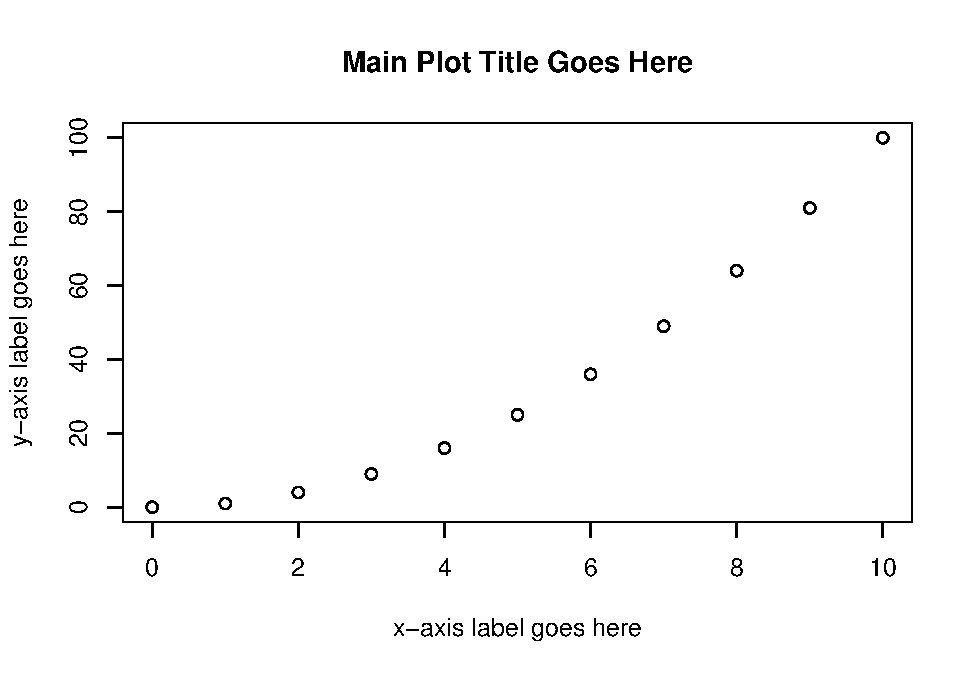
\includegraphics{au-r-workshop_files/figure-latex/unnamed-chunk-74-1} \end{center}

There are a few components:

\begin{itemize}
\tightlist
\item
  The \textbf{plotting region}: all data information is displayed here.
\item
  The \textbf{margin}: where axis labels, tick marks, and main plot
  titles are located
\item
  The \textbf{outer margin}: by default, there is no outer margin. You
  can add one if you want to add text here or make more room around the
  edges.
\end{itemize}

You can change just about everything there is about this plot to suit
your tastes. Duplicate this plot, but make the x-axis, y-axis, and main
titles something other than the placeholders shown here:

\begin{Shaded}
\begin{Highlighting}[]
\CommentTok{# plot dummy data}
\NormalTok{x =}\StringTok{ }\DecValTok{0}\OperatorTok{:}\DecValTok{10}
\NormalTok{y =}\StringTok{ }\NormalTok{x}\OperatorTok{^}\DecValTok{2}
\KeywordTok{plot}\NormalTok{(}\DataTypeTok{x =}\NormalTok{ x, }\DataTypeTok{y =}\NormalTok{ y,}
     \DataTypeTok{xlab =} \StringTok{"x-axis label goes here"}\NormalTok{, }
     \DataTypeTok{ylab =} \StringTok{"y-axis label goes here"}\NormalTok{,}
     \DataTypeTok{main =} \StringTok{"Main Plot Title Goes Here"}\NormalTok{)}
\end{Highlighting}
\end{Shaded}

Note that the first two arguments, \texttt{x} and \texttt{y}, specify
the coordinates of the points (i.e., the first point is placed at
coordinates \texttt{x{[}1{]}},\texttt{y{[}1{]}}). \texttt{plot()} has
\emph{tons} of arguments (or \emph{graphical parameters} as the help
file found using \texttt{?plot} or \texttt{?par} calls them) that change
how the plot looks. Note that when you want something displayed verbatim
on the plotting device, you must wrap that code in \texttt{"\ "}, i.e.,
the arguments \texttt{xlab}, \texttt{ylab}, and \texttt{main} all
receive a character vector of length 1 as input.

Table \ref{tab:plot-arg-table-pdf} shows information on just a handful
of them to get you started.

\begin{table}

\caption{\label{tab:plot-arg-table-pdf}Several of the key arguments to high- and low-level plotting functions}
\centering
\begin{threeparttable}
\begin{tabular}[t]{>{\ttfamily}l>{\ttfamily}l>{\raggedright\arraybackslash}p{25em}}
\toprule
Argument & Usage & Description\\
\midrule
xlab & xlab = "X-AXIS" & changes the x-axis label text\\
ylab & ylab = "Y-AXIS" & changes the y-axis label text\\
main & main = "TITLE" & changes the main title text\\
cex & cex = 1.5 & changes the size of symbols in the plotting region\\
pch & pch = 17 & changes the symbol type\\
\addlinespace
xlim & xlim = range(x) & changes the endpoints (limits) of the x-axis\\
ylim & ylim = c(0,1) & same as xlim, but for the y-axis\\
type & type = "l" & changes the way points are connected by lines\\
lty & lty = 2 & changes the line type\\
lwd & lwd = 2 & changes the line width\\
col & col = "blue" & changes the color of plotted objects\\
\bottomrule
\end{tabular}
\begin{tablenotes}
\item[a] cex is a multiplier: cex = 1.5 says make the points 1.5 times as large as they would be by default.
\item[b] There are approximately 20 different pch settings: pch = 1 is empty circles, pch = 16 is filled circles, etc.
\item[c] xlim and ylim both require a numeric vector of length 2 where neither of the elements may be an NA.
\item[d] The default is points only, type = "l" is for lines only, type = "o" is for points connected with lines, and type = "b" is for points and lines but with a small amount of separation between them.
\item[e] lty = 1 is solid, lty = 2 is dashed, lty = 3 is dotted, etc. You can also specific it like lty = "solid", lty = "dotted", or lty = "dotdash".
\item[f] works just like cex: lwd = 3 codes for a line that is 3 times as thick as it would normally be
\item[g] there is a whole host of colors you can pass R by name, run colors() to see for yourself
\end{tablenotes}
\end{threeparttable}
\end{table}

You are advised to try at least some of the arguments in Table
\ref{tab:plot-arg-table-pdf} out for yourself with your
\texttt{plot(x,\ y)} code from above - notice how every time you run
\texttt{plot()}, a whole new plot is created, not just the thing you
changed. There are definitely other options: check out \texttt{?plot} or
\texttt{?par} for more details.

\section{Lower Level Plotting
Functions}\label{lower-level-plotting-functions}

Now that you have a base plot designed to your liking, you might want to
add some additional ``layers'' to it to represent more data or other
kind of information like an additional label or text. Add some more
points to your plot by putting this line right beneath your
\texttt{plot(x,y)} code and run just the \texttt{points()} line (make
sure your device is showing a plot first):

\begin{Shaded}
\begin{Highlighting}[]
\CommentTok{# rev() reverses a vector: so the old x[1] is x[11] now}
\KeywordTok{points}\NormalTok{(}\DataTypeTok{x =} \KeywordTok{rev}\NormalTok{(x), }\DataTypeTok{y =}\NormalTok{ y, }\DataTypeTok{col =} \StringTok{"blue"}\NormalTok{, }\DataTypeTok{pch =} \DecValTok{16}\NormalTok{)}
\end{Highlighting}
\end{Shaded}

\begin{center}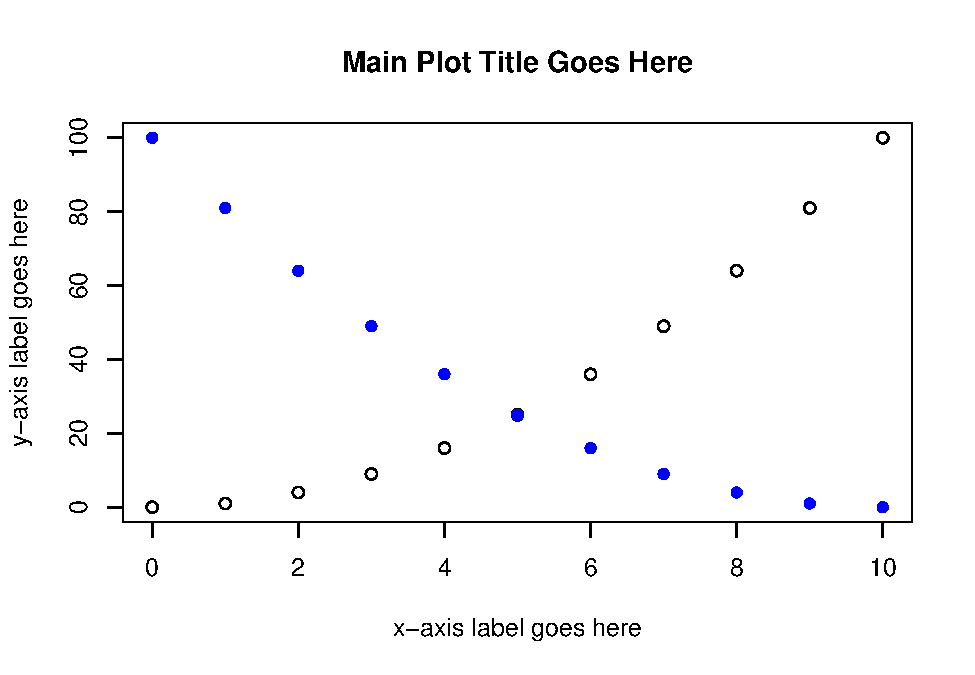
\includegraphics{au-r-workshop_files/figure-latex/unnamed-chunk-77-1} \end{center}

Here, \texttt{points()} acted like a low-level plotting function because
it added points to a plot you already made. Many of the arguments shown
in Table \ref{tab:plot-arg-table-pdf} can be used in both high-level and
low-level plotting functions (notice how \texttt{col} and \texttt{pch}
were used in \texttt{points()}). Just like \texttt{points()}, there is
also \texttt{lines()}:

\begin{Shaded}
\begin{Highlighting}[]
\KeywordTok{lines}\NormalTok{(}\DataTypeTok{x =}\NormalTok{ x, }\DataTypeTok{y =}\NormalTok{ x, }\DataTypeTok{lty =} \DecValTok{2}\NormalTok{, }\DataTypeTok{col =} \StringTok{"red"}\NormalTok{)}
\end{Highlighting}
\end{Shaded}

\begin{center}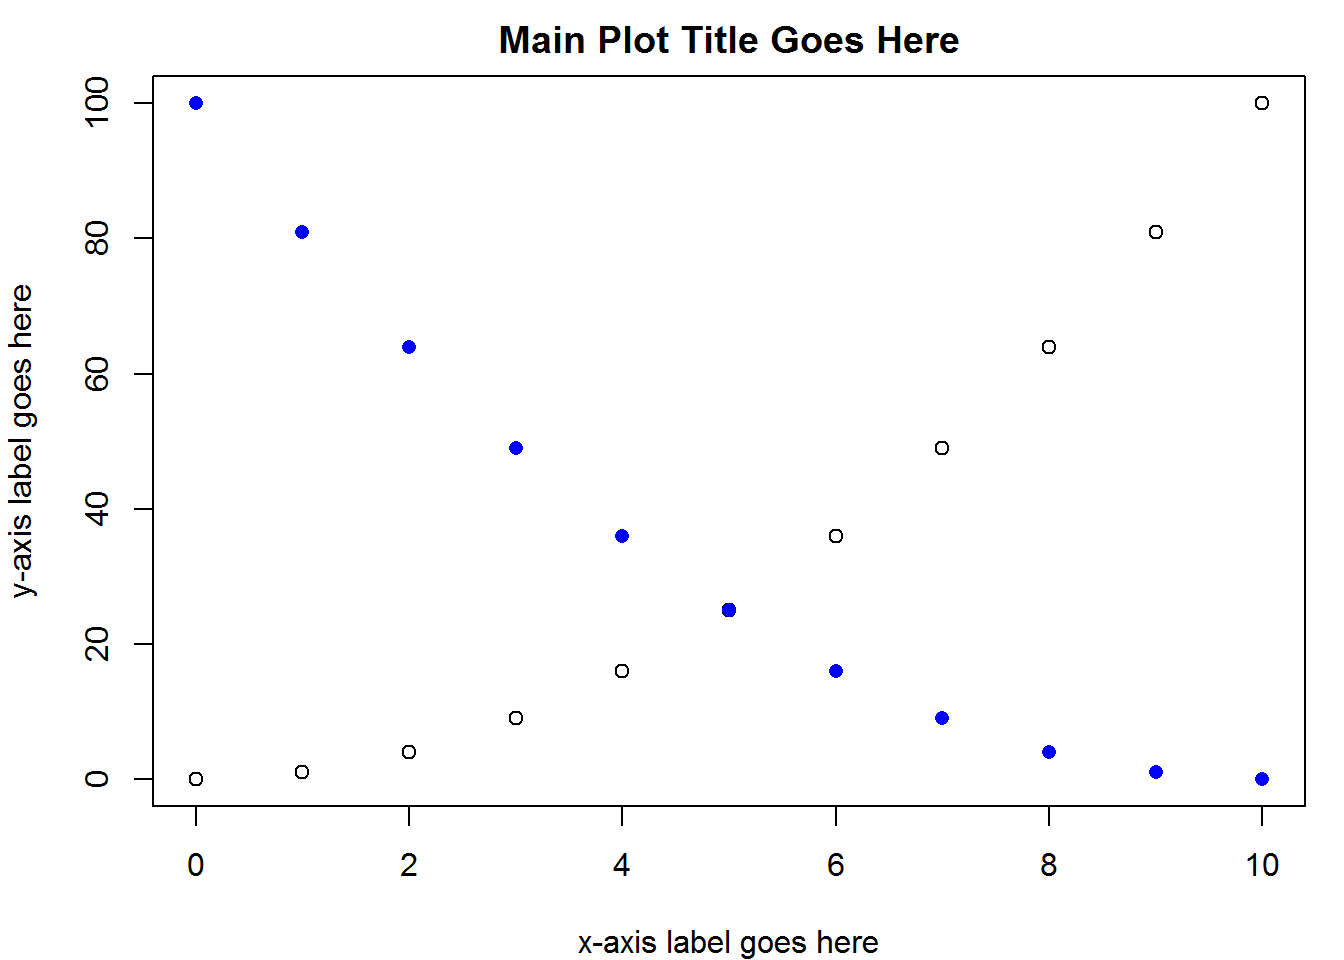
\includegraphics{au-r-workshop_files/figure-latex/unnamed-chunk-79-1} \end{center}

You can add text to the plotting region:

\begin{Shaded}
\begin{Highlighting}[]
\KeywordTok{text}\NormalTok{(}\DataTypeTok{x =} \DecValTok{5}\NormalTok{, }\DataTypeTok{y =} \DecValTok{80}\NormalTok{, }\StringTok{"This is Text"}\NormalTok{, }\DataTypeTok{cex =} \FloatTok{1.5}\NormalTok{, }\DataTypeTok{col =} \StringTok{"grey"}\NormalTok{, }\DataTypeTok{font =} \DecValTok{4}\NormalTok{)}
\end{Highlighting}
\end{Shaded}

\begin{center}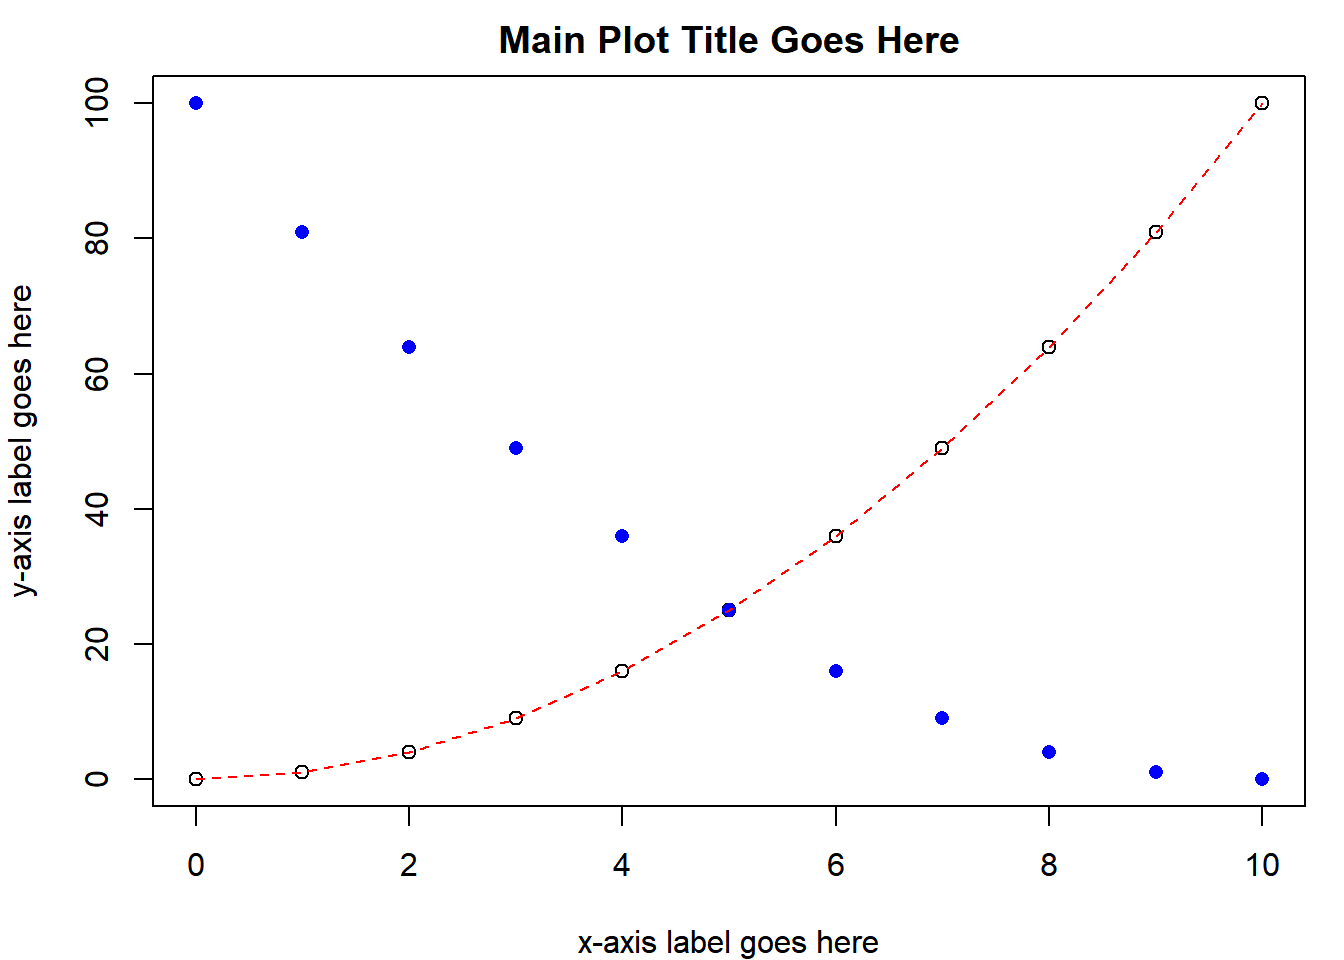
\includegraphics{au-r-workshop_files/figure-latex/unnamed-chunk-81-1} \end{center}

The text is centered on the coordinates you provide. You can also
provide vectors of coordinates and text to write different things at
once.

The easiest way to add a straight line to a plot is with
\texttt{abline()}. By default it takes two arguments: \texttt{a} and
\texttt{b} which are the intercept and slope, respectively, e.g.,
\texttt{abline(c(0,1))} will draw a 1:1 line. You can also do
\texttt{abline(h\ =\ 5)} to draw a horizontal line at 5 or
\texttt{abline(v\ =\ 5)} to draw a vertical line at \texttt{5}.

You can see that the text is centered on the coordinates
\texttt{x\ =\ 5} and \texttt{y\ =\ 80} using \texttt{abline()}:

\begin{Shaded}
\begin{Highlighting}[]
\KeywordTok{abline}\NormalTok{(}\DataTypeTok{h =} \DecValTok{80}\NormalTok{, }\DataTypeTok{col =} \StringTok{"grey"}\NormalTok{)}
\KeywordTok{abline}\NormalTok{(}\DataTypeTok{v =} \DecValTok{5}\NormalTok{, }\DataTypeTok{col =} \StringTok{"grey"}\NormalTok{)}
\end{Highlighting}
\end{Shaded}

\begin{center}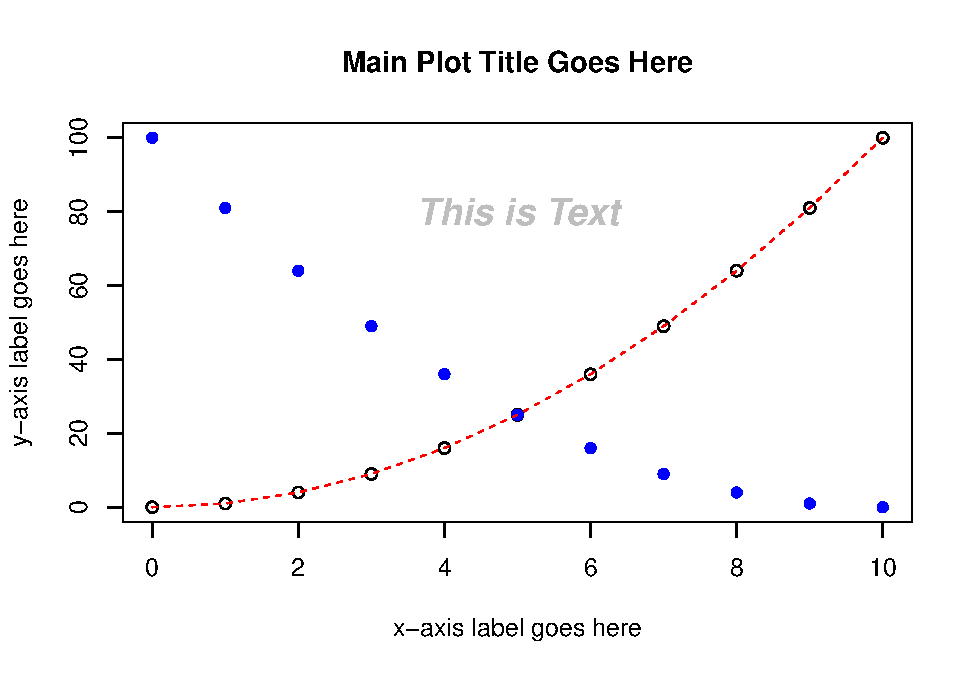
\includegraphics{au-r-workshop_files/figure-latex/unnamed-chunk-83-1} \end{center}

If you accidentally add a plot element that you don't want using a
low-level plotting function, the only way to remove it is by re-running
the high-level plotting function to start a new plot and adding only the
objects you want. Try removing the ``This is Text'' text and the
straight lines you drew with \texttt{abline()} from the plot displayed
in your device.

\section{Other High-Level Plotting
Functions}\label{other-high-level-plotting-functions}

You have just seen the basics of making two dimensional scatter plots
and line plots. You will now explore other types of graphs you can make.

\subsection{The Bar Graph}\label{the-bar-graph}

Another very common graph is a bar graph. R has a \texttt{bargraph()}
function, and again, it has lots of arguments. Here you will just make
two common variations: single bars per group and multiple bars per
group. Create a vector and plot it:

\begin{Shaded}
\begin{Highlighting}[]
\NormalTok{x1 =}\StringTok{ }\KeywordTok{c}\NormalTok{(}\DecValTok{2}\NormalTok{,}\DecValTok{4}\NormalTok{,}\DecValTok{6}\NormalTok{)}
\KeywordTok{barplot}\NormalTok{(x1)}
\end{Highlighting}
\end{Shaded}

\begin{center}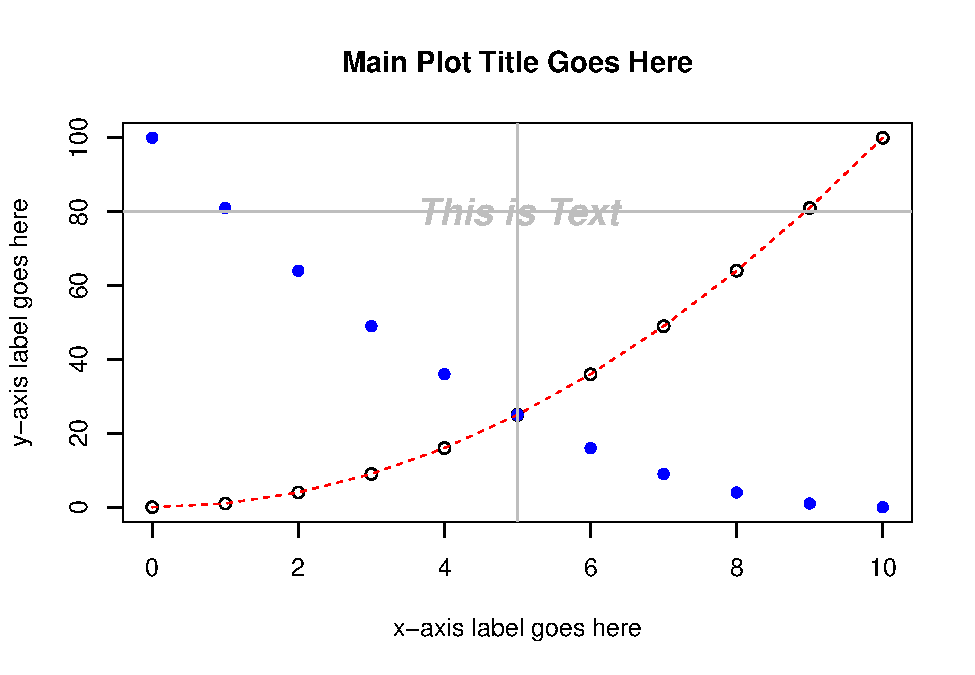
\includegraphics{au-r-workshop_files/figure-latex/unnamed-chunk-84-1} \end{center}

Notice that there are no group names on the bars (if \texttt{x1} had
names, there would be). You can add names by using the argument
\texttt{names.arg}:

\begin{Shaded}
\begin{Highlighting}[]
\KeywordTok{barplot}\NormalTok{(x1, }\DataTypeTok{names.arg =} \KeywordTok{c}\NormalTok{(}\StringTok{"a"}\NormalTok{, }\StringTok{"b"}\NormalTok{, }\StringTok{"c"}\NormalTok{))}
\end{Highlighting}
\end{Shaded}

Add some more information by including two bars per group. Create
another vector and combine it with the old data:

\begin{Shaded}
\begin{Highlighting}[]
\NormalTok{x2 =}\StringTok{ }\KeywordTok{c}\NormalTok{(}\DecValTok{3}\NormalTok{,}\DecValTok{5}\NormalTok{,}\DecValTok{7}\NormalTok{)}
\NormalTok{x3 =}\StringTok{ }\KeywordTok{rbind}\NormalTok{(x1, x2)}
\KeywordTok{barplot}\NormalTok{(x3, }\DataTypeTok{names.arg =} \KeywordTok{c}\NormalTok{(}\StringTok{"a"}\NormalTok{, }\StringTok{"b"}\NormalTok{, }\StringTok{"c"}\NormalTok{), }\DataTypeTok{beside =}\NormalTok{ T)}
\end{Highlighting}
\end{Shaded}

\begin{center}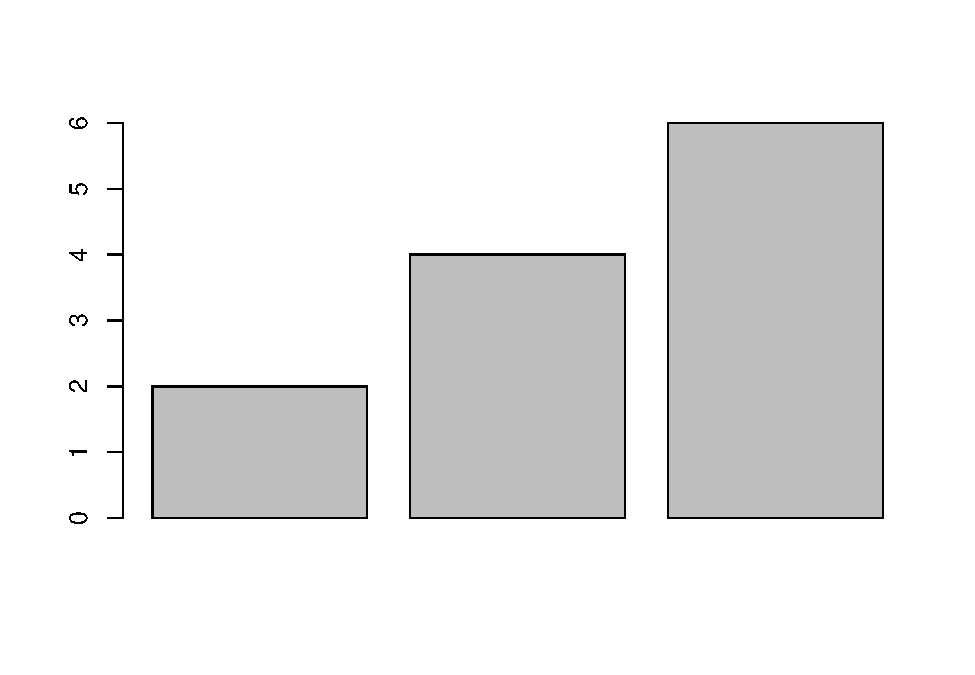
\includegraphics{au-r-workshop_files/figure-latex/unnamed-chunk-86-1} \end{center}

To add multiple bars per group, R needs a matrix like you just made. The
\textbf{columns} store the heights of the bars that will be placed
together in a group. Including the \texttt{beside\ =\ T} argument tells
R to plot all groups as different bars as opposed to using a stacked bar
graph.

Oftentimes, you will want to add error bars to a bar graph like this. To
avoid digressing too much here, creating error bars is covered as a
bonus topic (Section \ref{error-bars}).

\section{Box-and-Whisker Plots}\label{box-whisker}

Box-and-whisker plots are a great way to visualize the spread of your
data. All you need to make a box-and-whisker plot is a grouping variable
(a factor, revisit Section \ref{factors} if you don't remember what
these are) and some continuous (i.e., numeric) data for each level of
the factor. You will be using the \texttt{creel.csv} data set (see the
\protect\hyperlink{data-sets}{instructions} on acquiring and placing the
data files in the appropriate location).

Read the data in and print a summary:

\begin{Shaded}
\begin{Highlighting}[]
\NormalTok{dat =}\StringTok{ }\KeywordTok{read.csv}\NormalTok{(}\StringTok{"../Data/creel.csv"}\NormalTok{)}
\KeywordTok{summary}\NormalTok{(dat)}
\end{Highlighting}
\end{Shaded}

\begin{verbatim}
##            fishery        hours       
##  Harvest       :100   Min.   :-1.150  
##  Non.Tournament:100   1st Qu.: 9.936  
##  Tournament    :100   Median :20.758  
##                       Mean   :26.050  
##                       3rd Qu.:43.896  
##                       Max.   :62.649
\end{verbatim}

This data set contains some simulated (i.e., fake) continuous and
categorical data that represent 300 anglers who were creel
surveyed\footnote{A creel survey is a sampling program where fishers are
  asked questions about their fishing behavior in order to estimate
  effort and harvest.}. In the data set, there are three categories
(levels to the factor \texttt{fishery}) and the continuous variable is
how many hours each angler fished this year. If you supply the generic
\texttt{plot()} function with a continuous response (\texttt{y})
variable and a categorical predictor (\texttt{x}) variable, it will
automatically assume you want to make a box-and-whisker plot:

\begin{Shaded}
\begin{Highlighting}[]
\KeywordTok{plot}\NormalTok{(}\DataTypeTok{x =}\NormalTok{ dat}\OperatorTok{$}\NormalTok{fishery, }\DataTypeTok{y =}\NormalTok{ dat}\OperatorTok{$}\NormalTok{hours)}
\end{Highlighting}
\end{Shaded}

\begin{center}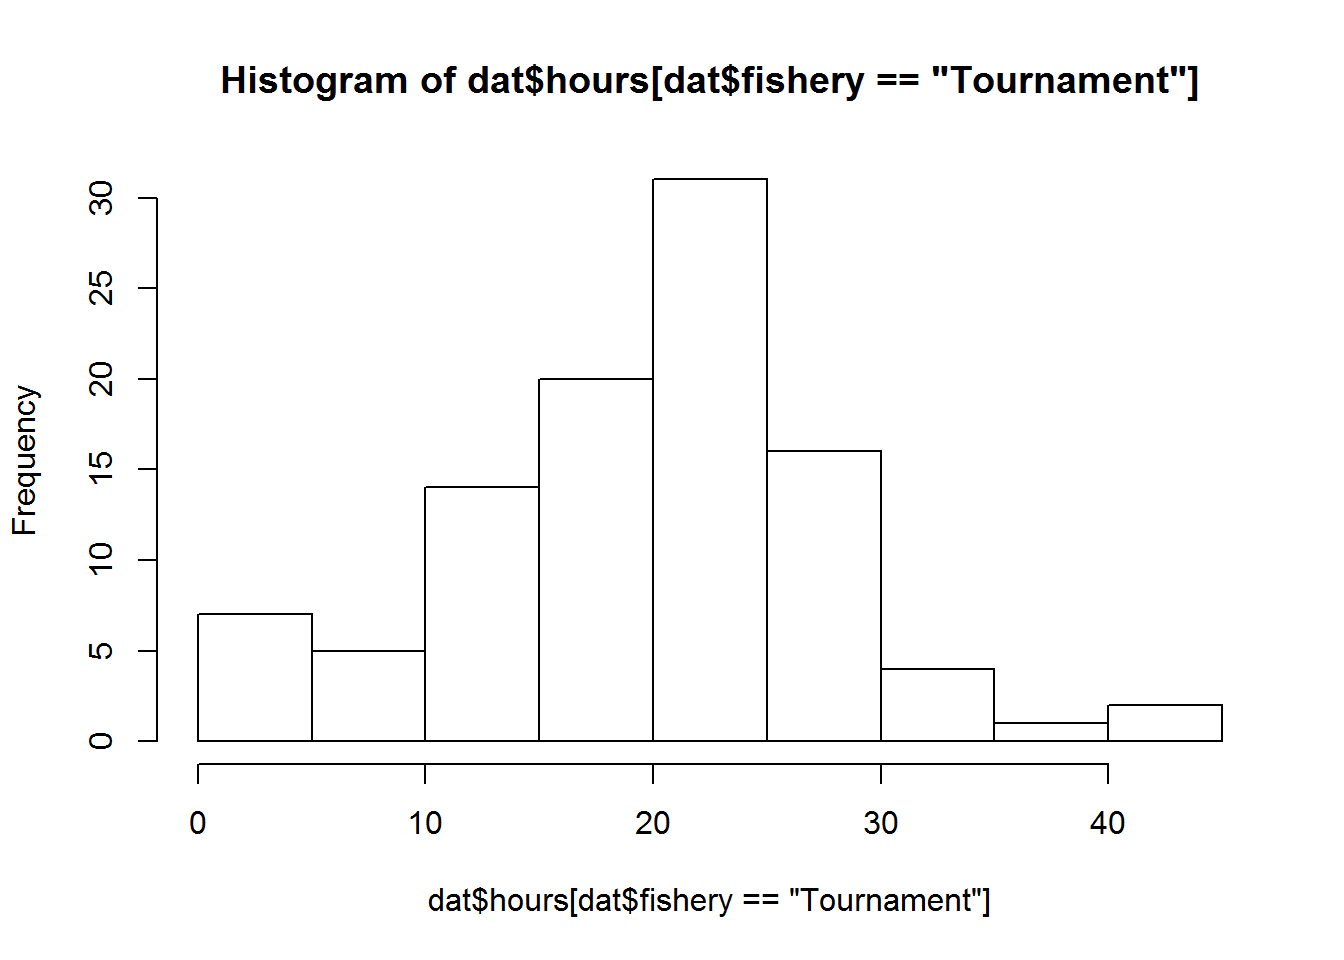
\includegraphics{au-r-workshop_files/figure-latex/unnamed-chunk-89-1} \end{center}

In the box-and-whisker plot above, the heavy line is the median, the
ends of the boxes are the 25\textsuperscript{th} and
75\textsuperscript{th} percentiles and the ``whiskers'' are the
2.5\textsuperscript{th} and 97.5\textsuperscript{th} percentiles. Any
points that are outliers (i.e., fall outside of the whiskers) will be
shown as points\footnote{Outliers can be turned off using the
  \texttt{outline\ =\ F} argument to the \texttt{plot()} function}.

It is worth introducing a shorthand syntax of typing the same command:

\begin{Shaded}
\begin{Highlighting}[]
\KeywordTok{plot}\NormalTok{(hours }\OperatorTok{~}\StringTok{ }\NormalTok{fishery, }\DataTypeTok{data =}\NormalTok{ dat)}
\end{Highlighting}
\end{Shaded}

Instead of saying \texttt{plot(x\ =\ x.var,\ y\ =\ y.var)}, this
expression says \texttt{plot(y.var\ \textasciitilde{}\ x.var)}. The
\texttt{\textasciitilde{}} reads ``as a function of''. By specifying the
\texttt{data} argument, you no longer need to indicate where the
variables \texttt{hours} and \texttt{fishery} are found. Many R
functions have a \texttt{data} argument that works this same way. It is
sometimes preferable to plot variables with this syntax because it is
often less code and is also the format of R's statistical
equations\footnote{Which allows you to easily copy and paste the code
  between the model and plot functions, see Chapter \ref{ch3}}.

\section{Histograms}\label{histograms}

Another way to show the distribution of a variable is with histograms.
These figures show the relative frequencies of observations in different
discrete bins. Make a histogram for the hours the surveyed tournament
anglers fished this year:

\begin{Shaded}
\begin{Highlighting}[]
\KeywordTok{hist}\NormalTok{(dat}\OperatorTok{$}\NormalTok{hours[dat}\OperatorTok{$}\NormalTok{fishery }\OperatorTok{==}\StringTok{ "Tournament"}\NormalTok{])}
\end{Highlighting}
\end{Shaded}

\begin{center}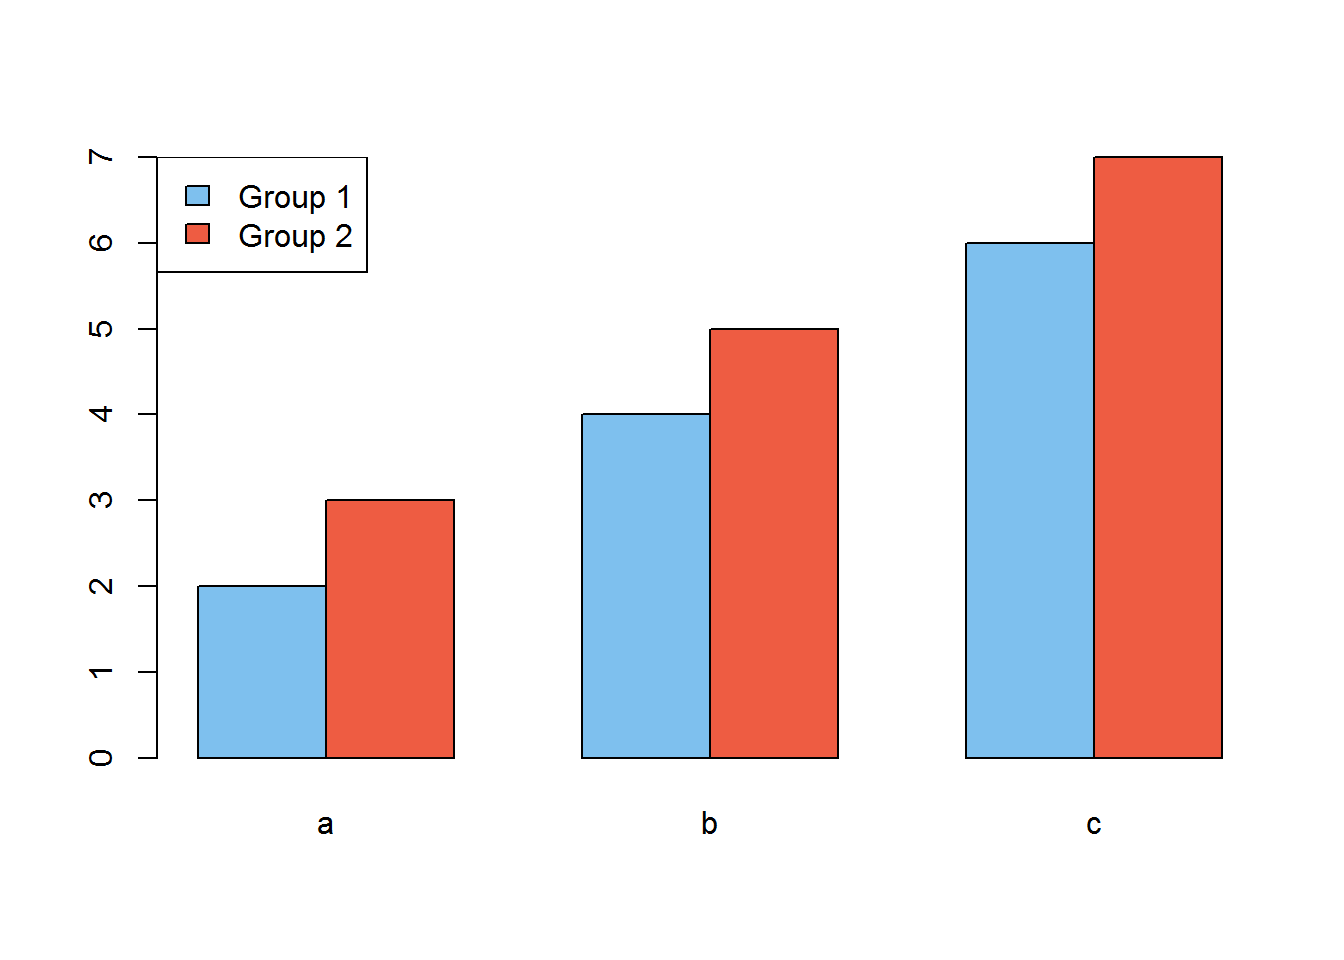
\includegraphics{au-r-workshop_files/figure-latex/unnamed-chunk-91-1} \end{center}

Notice the subset that extracts hours fished for tournament anglers only
before plotting.

\texttt{hist()} automatically selects the number of bins based on the
range and resolution of the data. You can specify how many evenly-sized
bins you want to plot:

\begin{Shaded}
\begin{Highlighting}[]
\CommentTok{# extract the hours for tournament anglers}
\NormalTok{t_hrs =}\StringTok{ }\NormalTok{dat}\OperatorTok{$}\NormalTok{hours[dat}\OperatorTok{$}\NormalTok{fishery }\OperatorTok{==}\StringTok{ "Tournament"}\NormalTok{]}

\CommentTok{# create the bin endpoints}
\NormalTok{nbins =}\StringTok{ }\DecValTok{20}
\NormalTok{breaks =}\StringTok{ }\KeywordTok{seq}\NormalTok{(}\DataTypeTok{from =} \KeywordTok{min}\NormalTok{(t_hrs), }\DataTypeTok{to =} \KeywordTok{max}\NormalTok{(t_hrs), }\DataTypeTok{length =}\NormalTok{ nbins }\OperatorTok{+}\StringTok{ }\DecValTok{1}\NormalTok{)}
\KeywordTok{hist}\NormalTok{(t_hrs, }\DataTypeTok{breaks =}\NormalTok{ breaks, }\DataTypeTok{main =} \StringTok{"Tournament"}\NormalTok{, }\DataTypeTok{col =} \StringTok{"grey"}\NormalTok{)}
\end{Highlighting}
\end{Shaded}

\begin{center}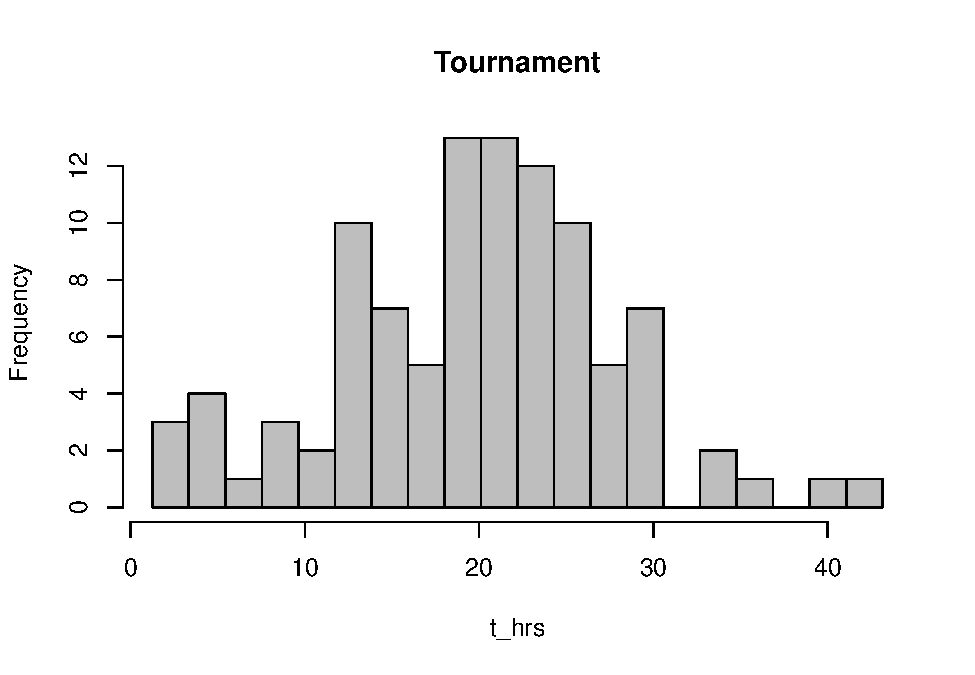
\includegraphics{au-r-workshop_files/figure-latex/unnamed-chunk-92-1} \end{center}

\section{\texorpdfstring{The \texttt{par}
Function}{The par Function}}\label{the-par-function}

If it bothers you that the axes are ``floating'', you can fix this using
this command:

\begin{Shaded}
\begin{Highlighting}[]
\KeywordTok{par}\NormalTok{(}\DataTypeTok{xaxs =} \StringTok{"i"}\NormalTok{, }\DataTypeTok{yaxs =} \StringTok{"i"}\NormalTok{)}
\KeywordTok{hist}\NormalTok{(t_hrs, }\DataTypeTok{breaks =}\NormalTok{ breaks, }\DataTypeTok{main =} \StringTok{"Tournament"}\NormalTok{, }\DataTypeTok{col =} \StringTok{"grey"}\NormalTok{)}
\end{Highlighting}
\end{Shaded}

\begin{center}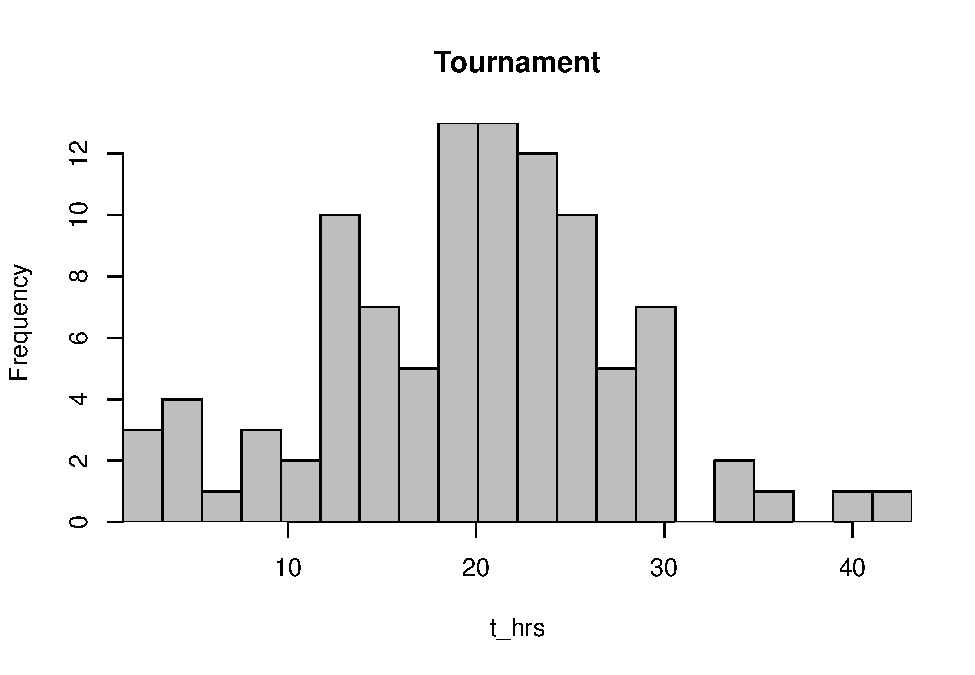
\includegraphics{au-r-workshop_files/figure-latex/unnamed-chunk-93-1} \end{center}

Here, you changed the graphical parameters of the graphics device by
using the \texttt{par()} function. Once you change the settings in
\texttt{par()}, they will remain that way until you start a new device.

The \texttt{par()} function is central to fine-tuning your graphics.
Here, the \texttt{xaxs\ =\ "i"} and \texttt{yaxs\ =\ "i"} arguments
essentially removed the buffer between the data and the axes.
\texttt{par()} has options to change the size of the margins, add outer
margins, change colors, etc. Some of the graphical parameters that can
be passed to high- and low-level plotting functions (like those in Table
\ref{tab:plot-arg-table-pdf}) can also be passed \texttt{par()}. Check
out the help file (\texttt{?par}) to see everything it can do. If you
want to start over with fresh \texttt{par()} settings, start a new
device.

\section{New Temporary Devices}\label{new-temporary-devices}

If you are using RStudio, then likely all of the plots you have made
thus far have shown up in the lower right-hand corner or your RStudio
window. You have been using RStudio's built-in plotting device. If you
wish to open a new plotting device (maybe to put it on a separate
monitor), you can use the following commands, depending on your
operating system:

\begin{itemize}
\tightlist
\item
  \textbf{Windows Users} -- just run \texttt{windows()} to open up a new
  plotting device. It will become the active device.
\item
  \textbf{Mac Users} -- similarly, you can run \texttt{quartz()} to open
  a new device.
\item
  \textbf{Linux Users} -- similarly, just run \texttt{x11()}.
\end{itemize}

\section{Multi-panel Plots}\label{multi-panel-plots}

Sometimes you want to display more than one plot at a time. You can make
a multi-panel plot which allows for multiple plotting regions to show up
simultaneously within the same plotting device. First, you need to
change the layout of the plotting region. The easiest way to set up the
device for multi-panel plotting is by using the \texttt{mfrow} argument
in the \texttt{par()} function.

Below, the code says ``set up the graphical parameters so that there is
1 row and 3 columns of plotting regions within the device''. Every time
you make a new plot, it will go in the next available plotting region.
Make 3 histograms, each that represents a different sector of the
fishery:

\begin{Shaded}
\begin{Highlighting}[]
\KeywordTok{par}\NormalTok{(}\DataTypeTok{mfrow =} \KeywordTok{c}\NormalTok{(}\DecValTok{1}\NormalTok{,}\DecValTok{3}\NormalTok{))}
\KeywordTok{sapply}\NormalTok{(}\KeywordTok{levels}\NormalTok{(dat}\OperatorTok{$}\NormalTok{fishery), }\ControlFlowTok{function}\NormalTok{(f) \{}
  \KeywordTok{hist}\NormalTok{(dat}\OperatorTok{$}\NormalTok{hours[dat}\OperatorTok{$}\NormalTok{fishery }\OperatorTok{==}\StringTok{ }\NormalTok{f], }\DataTypeTok{main =}\NormalTok{ f, }\DataTypeTok{xlab =} \StringTok{""}\NormalTok{)}
\NormalTok{\})}
\end{Highlighting}
\end{Shaded}

\begin{center}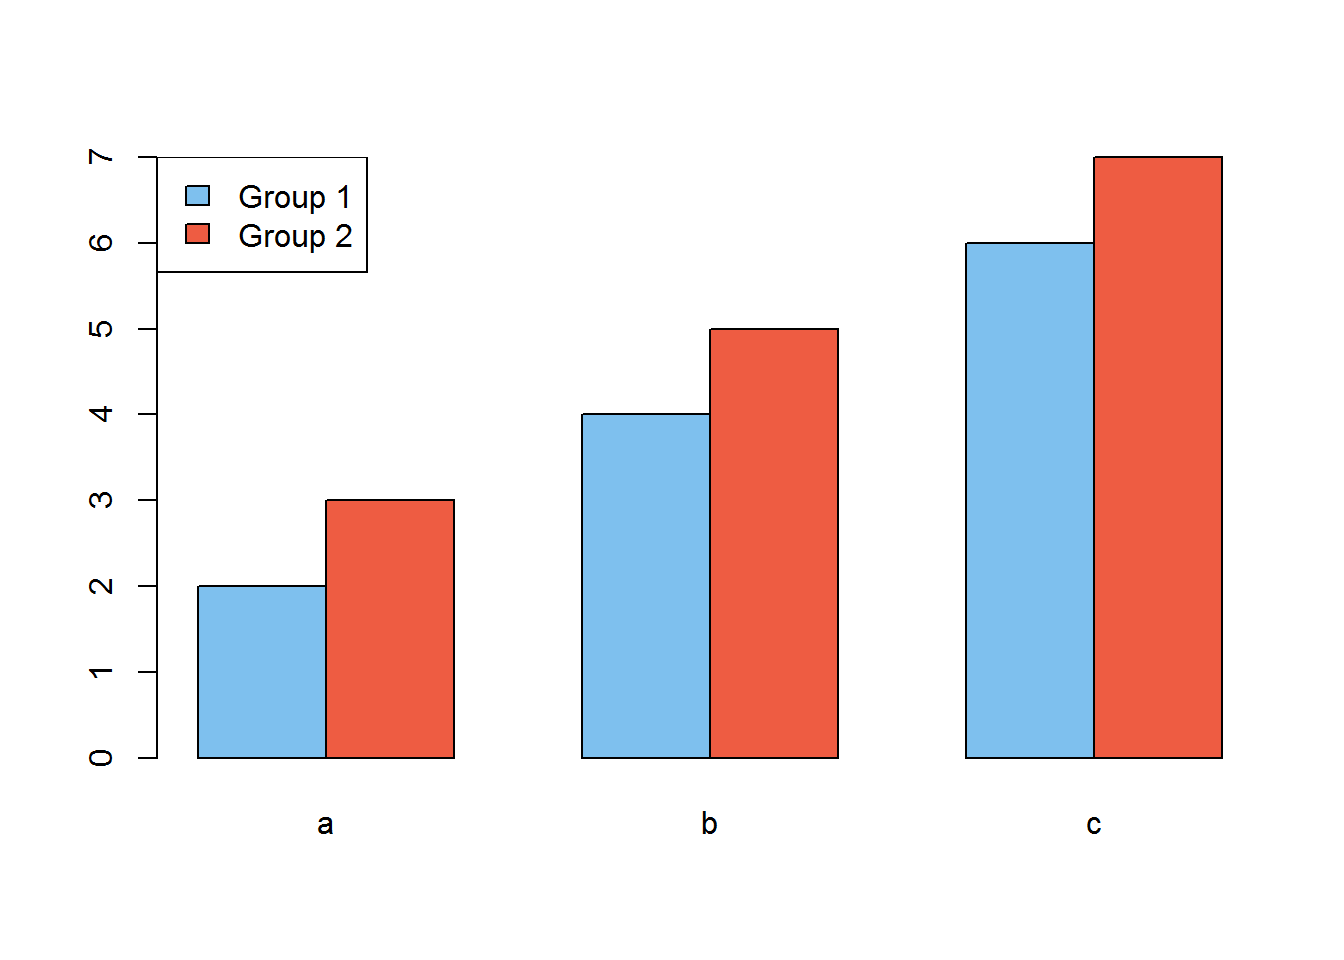
\includegraphics{au-r-workshop_files/figure-latex/unnamed-chunk-95-1} \end{center}

Here, \texttt{sapply()} applied a user-defined function that plots a
histogram for a given fishery type to each of the fishery types
separately\footnote{\texttt{sapply()} works like \texttt{apply()},
  except on vectors only so you don't need to supply it with a
  \texttt{1} or \texttt{2} for rows or columns}, which allowed you to
only need to type the \texttt{hist()} code once. There are other ways to
make multi-panel plots, however, they are beyond the scope of this
introductory material. See \texttt{?layout} for details. With this
function you can change the size of certain plots and make them have
different shapes (i.e., some squares, some rectangles, etc.), but it
takes some pretty involved (though not impossible, by any means)
specification of how you want the device to be split up into regions.

\section{Legends}\label{legends}

Oftentimes you will want to add a legend to plots to help people
interpret what it is showing. You can add legends to R plots using the
low-level plotting function \texttt{legend()}. Add a legend to the bar
plot you made earlier with two groups. First, re-make the plot by
running the high-level \texttt{barplot()} function, but change the
colors of the bars to be shades of blue and red. Once you have the plot
made, add the legend:

\begin{Shaded}
\begin{Highlighting}[]
\KeywordTok{barplot}\NormalTok{(x3, }\DataTypeTok{beside =}\NormalTok{ T, }
        \DataTypeTok{names.arg =} \KeywordTok{c}\NormalTok{(}\StringTok{"a"}\NormalTok{, }\StringTok{"b"}\NormalTok{, }\StringTok{"c"}\NormalTok{),}
        \DataTypeTok{col =} \KeywordTok{c}\NormalTok{(}\StringTok{"skyblue2"}\NormalTok{, }\StringTok{"tomato2"}\NormalTok{))}
\KeywordTok{legend}\NormalTok{(}\StringTok{"topleft"}\NormalTok{, }\DataTypeTok{legend =} \KeywordTok{c}\NormalTok{(}\StringTok{"Group 1"}\NormalTok{, }\StringTok{"Group 2"}\NormalTok{),}
       \DataTypeTok{fill =} \KeywordTok{c}\NormalTok{(}\StringTok{"skyblue2"}\NormalTok{, }\StringTok{"tomato2"}\NormalTok{))}
\end{Highlighting}
\end{Shaded}

\begin{center}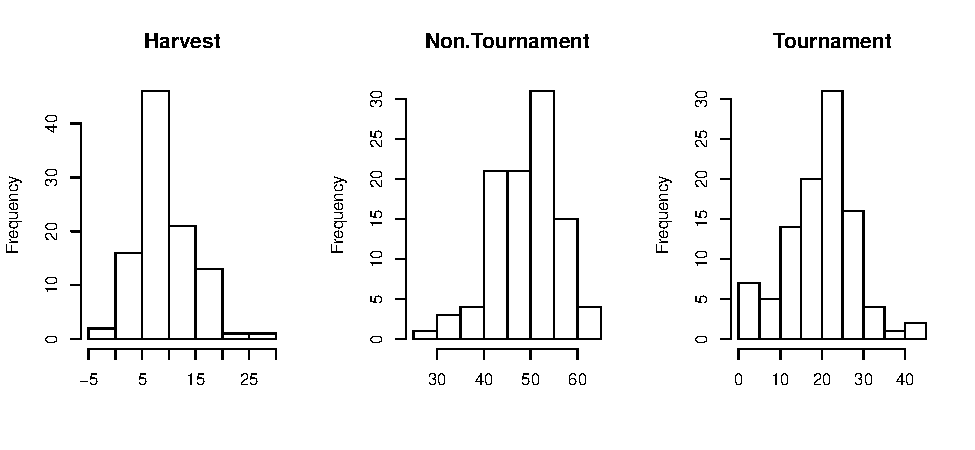
\includegraphics{au-r-workshop_files/figure-latex/unnamed-chunk-96-1} \end{center}

The box can be removed using the \texttt{bty\ =\ "n"} argument and the
size can be changed using \texttt{cex}. The position can be specified
either with words (like above) or by using x-y coordinates.

Here is a more complex example:

\begin{Shaded}
\begin{Highlighting}[]
\CommentTok{# 1) extract and sort the hours for two fisheries from fewest hours}
\NormalTok{t_hrs =}\StringTok{ }\KeywordTok{sort}\NormalTok{(dat}\OperatorTok{$}\NormalTok{hours[dat}\OperatorTok{$}\NormalTok{fishery }\OperatorTok{==}\StringTok{ "Tournament"}\NormalTok{])}
\NormalTok{n_hrs =}\StringTok{ }\KeywordTok{sort}\NormalTok{(dat}\OperatorTok{$}\NormalTok{hours[dat}\OperatorTok{$}\NormalTok{fishery }\OperatorTok{==}\StringTok{ "Non.Tournament"}\NormalTok{])}

\CommentTok{# 2) make the plot: plot for t_hrs only, but ensure xlim covers both groups}
\CommentTok{# set the margins: }
  \CommentTok{# 4 lines of margin space on bottom and left,}
  \CommentTok{# 1 on top and right}
\KeywordTok{par}\NormalTok{(}\DataTypeTok{mar =} \KeywordTok{c}\NormalTok{(}\DecValTok{4}\NormalTok{,}\DecValTok{4}\NormalTok{,}\DecValTok{1}\NormalTok{,}\DecValTok{1}\NormalTok{))  }
\KeywordTok{plot}\NormalTok{(}\DataTypeTok{x =}\NormalTok{ t_hrs, }\DataTypeTok{y =} \DecValTok{1}\OperatorTok{:}\KeywordTok{length}\NormalTok{(t_hrs),}
     \DataTypeTok{type =} \StringTok{"o"}\NormalTok{, }\DataTypeTok{lty =} \DecValTok{2}\NormalTok{, }\DataTypeTok{xlim =} \KeywordTok{range}\NormalTok{(}\KeywordTok{c}\NormalTok{(t_hrs, n_hrs)),}
     \DataTypeTok{xlab =} \StringTok{"Hours Fished/Year"}\NormalTok{, }\DataTypeTok{ylab =} \StringTok{"Rank within Fishery Samples"}\NormalTok{,}
     \DataTypeTok{las =} \DecValTok{1}\NormalTok{)  }\CommentTok{# las = 1 says "turn the y-axis tick labels to be horizontal"}
\CommentTok{# 3) add info for the other fishery}
\KeywordTok{points}\NormalTok{(}\DataTypeTok{x =}\NormalTok{ n_hrs, }\DataTypeTok{y =} \DecValTok{1}\OperatorTok{:}\KeywordTok{length}\NormalTok{(n_hrs), }\DataTypeTok{type =} \StringTok{"o"}\NormalTok{, }\DataTypeTok{lty =} \DecValTok{1}\NormalTok{, }\DataTypeTok{pch =} \DecValTok{16}\NormalTok{)}
\CommentTok{# 4) add the legend}
\KeywordTok{legend}\NormalTok{(}\StringTok{"topleft"}\NormalTok{, }\DataTypeTok{legend =} \KeywordTok{c}\NormalTok{(}\StringTok{"Tournament"}\NormalTok{, }\StringTok{"Non-Tournament"}\NormalTok{), }
       \DataTypeTok{lty =} \KeywordTok{c}\NormalTok{(}\DecValTok{2}\NormalTok{,}\DecValTok{1}\NormalTok{), }\DataTypeTok{pch =} \KeywordTok{c}\NormalTok{(}\DecValTok{1}\NormalTok{, }\DecValTok{16}\NormalTok{), }\DataTypeTok{bty =} \StringTok{"n"}\NormalTok{)}
\end{Highlighting}
\end{Shaded}

\begin{center}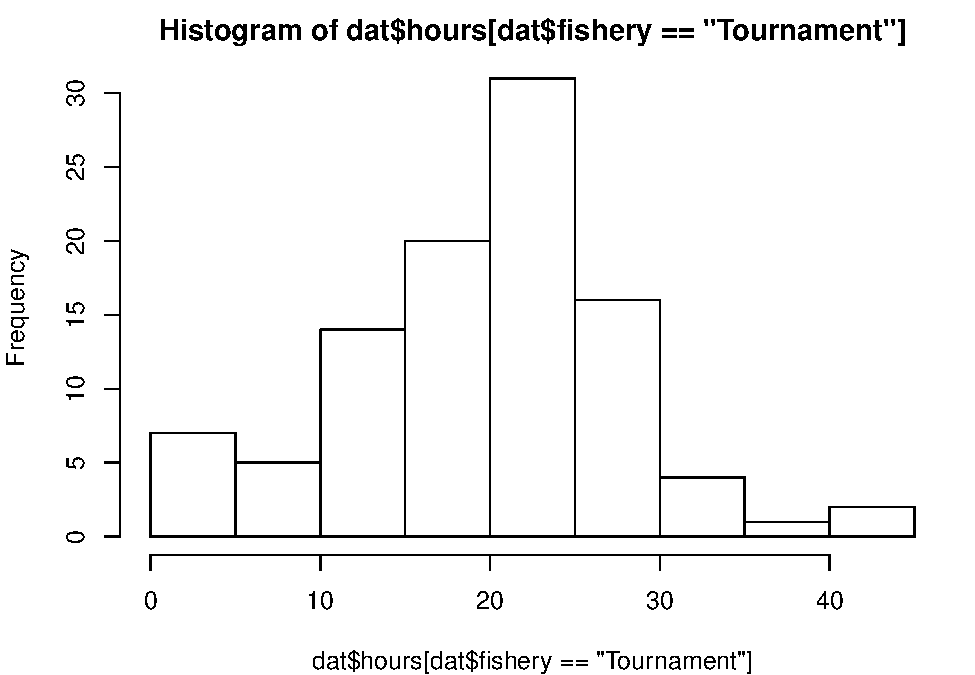
\includegraphics{au-r-workshop_files/figure-latex/unnamed-chunk-97-1} \end{center}

Notice that you need to be careful about the order of how you specify
which \texttt{lty} and \texttt{pch} settings match up with the elements
of the \texttt{legend} argument. In the \texttt{plot()} code, you
specified that the \texttt{lty\ =\ 2} but didn't specify what
\texttt{pch} should be (it defaults to \texttt{1}). So when you put the
``Tournament'' group first the the \texttt{legend} argument vector, you
must be sure to use the corresponding plotting codes. The first element
of the \texttt{lty} argument matches up with the first element of
\texttt{legend}, and so on. Note the other plotting tricks used in the
code above: changing the margins using \texttt{par(mar)} and the
rotation of y-axis tick mark labels using \texttt{las\ =\ 1}.

\section{Exporting Plots}\label{exporting-plots}

There are two main ways to save plots. First is a quick-and-dirty method
that saves the plots, but they are not high-resolution and you can't
automate this process. The second method produces cleaner-looking
high-resolution plots with code that can be embedded in your script,
ensuring the same exact plot will be created each time the code is
executed

\subsection{Click Save}\label{click-save}

\begin{itemize}
\tightlist
\item
  If your plot is in the RStudio built-in graphics device: Right above
  the plot, click \emph{Export \textgreater{} Save as Image}. Change the
  name, dimensions and file type.
\item
  If your plot is in a plotting device window (opened with
  \texttt{windows()} or \texttt{quartz()}: Simply go to \emph{File
  \textgreater{} Save}.
\end{itemize}

All plots will be saved in the working directory by default. You can
also just copy the plot to your clipboard (\emph{File \textgreater{}
Copy to the clipboard \textgreater{} bitmap}) and paste it where you
want. You should saving one of the plots you made in this Chapter using
this approach.

\subsection{Use a function to place plot in a new
file}\label{use-a-function-to-place-plot-in-a-new-file}

If you are producing plots for a final report or publication, you want
the output to be as clean-looking as possible and you want them to be
fully reproducible so when something changes with your data or analysis
in review, you can reproduce the same figure with the new results. You
can save high-resolution plots through R by using the following steps:

\begin{Shaded}
\begin{Highlighting}[]
\CommentTok{# step 1: Make a pixels per inch object}
\NormalTok{ppi =}\StringTok{ }\DecValTok{600}

\CommentTok{# step 2: Call the figure file creation function}
\KeywordTok{png}\NormalTok{(}\StringTok{"TestFigure.png"}\NormalTok{, }\DataTypeTok{h =} \DecValTok{8} \OperatorTok{*}\StringTok{ }\NormalTok{ppi, }\DataTypeTok{w =} \DecValTok{8} \OperatorTok{*}\StringTok{ }\NormalTok{ppi, }\DataTypeTok{res =}\NormalTok{ ppi)}

\CommentTok{# step 3: Run the plot }
\CommentTok{# put all of your plotting code here (without windows())}

\CommentTok{# step 4: Close the device}
\KeywordTok{dev.off}\NormalTok{()}
\end{Highlighting}
\end{Shaded}

A plot will be saved in your working directory containing the plot made
by the code in step 3 above. The \texttt{ppi} object is pixels-per-inch.
When you specify \texttt{h\ =\ 8\ *\ ppi}, you are saying ``make a plot
with height equal to 8 inches''. There are similar functions to make
PDFs, tiff files, jpegs, etc. You should try saving one of the plots you
made in this Chapter using this approach.

\section{Bonus Topic: Error Bars}\label{error-bars}

Rarely should you ever present estimates without some measure of
uncertainty. The most common way for visualizing the uncertainty in an
estimate is by using error bars, which can be added to an R plot using
the lower-level function \texttt{arrows()}. To use \texttt{arrows()},
you need:

\begin{itemize}
\tightlist
\item
  Vectors of the \texttt{x} and \texttt{y} coordinates of the lower
  bound of the error bars
\item
  Vectors of the \texttt{x} and \texttt{y} coordinates of the upper
  bound of the error bars
\end{itemize}

The syntax for \texttt{arrows()} is as follows:
\texttt{arrows(x0,\ y0,\ x1,\ y1,\ ...)}, where \texttt{x0} and
\texttt{y0} are the coordinates you are drawing ``from'' (e.g., lower
limits) and the \texttt{x1} and \texttt{y1} are the coordinates you are
drawing ``to'' (e.g., upper limits). The \texttt{...} represents other
arguments to change how the error bars look. Calculate the mean of the
different fishery sectors (if you don't remember how \texttt{tapply()}
works, revisit Section \ref{data-summaries}) and plot them:

\begin{Shaded}
\begin{Highlighting}[]
\NormalTok{x_bar =}\StringTok{ }\KeywordTok{tapply}\NormalTok{(dat}\OperatorTok{$}\NormalTok{hours, dat}\OperatorTok{$}\NormalTok{fishery, mean)}
\KeywordTok{barplot}\NormalTok{(x_bar)}
\end{Highlighting}
\end{Shaded}

\begin{center}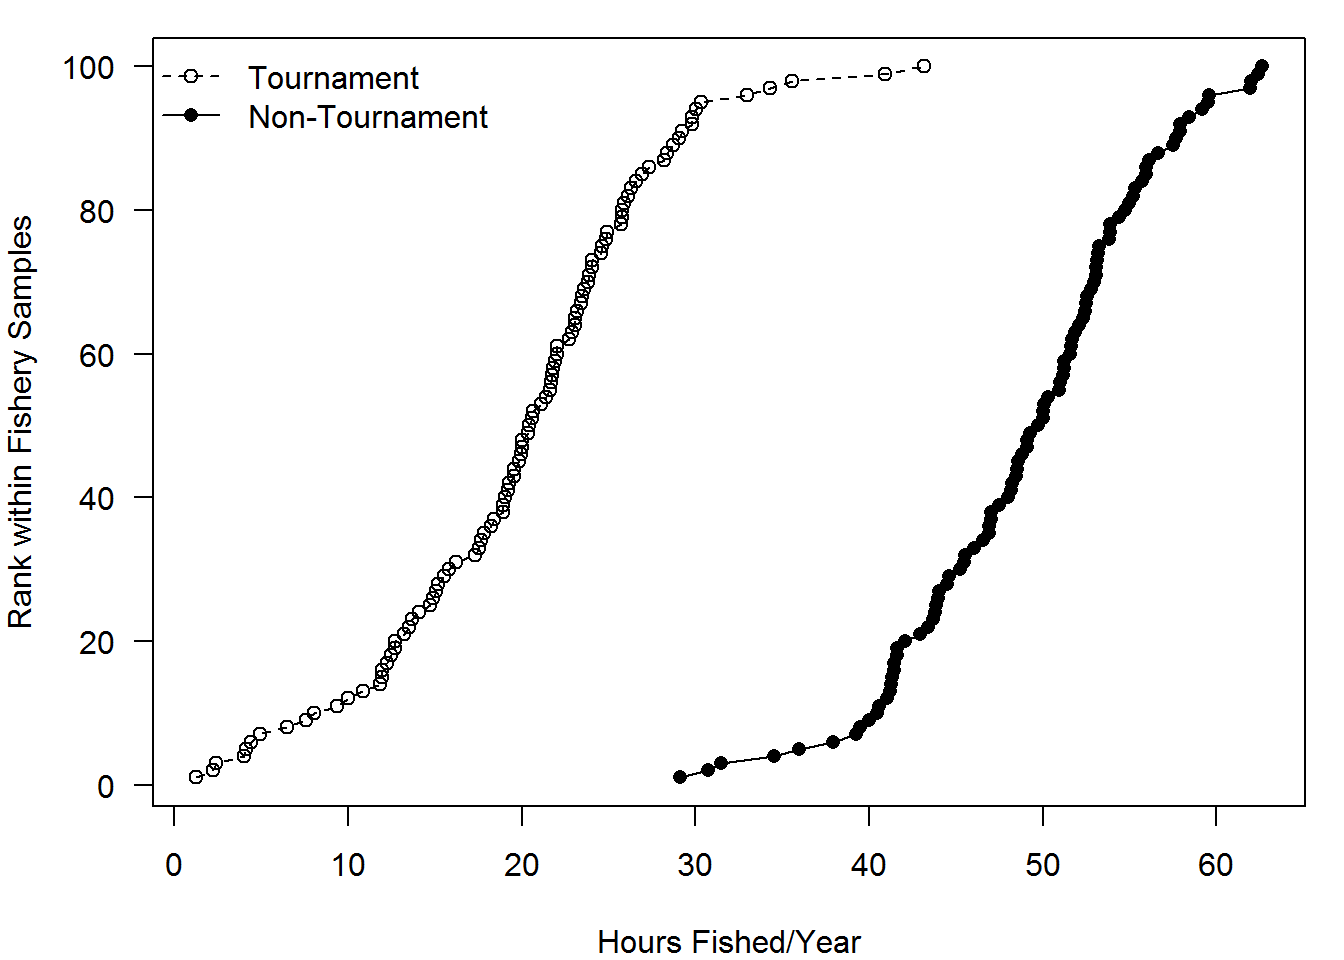
\includegraphics{au-r-workshop_files/figure-latex/unnamed-chunk-99-1} \end{center}

You wish to add error bars that represent 95\% confidence intervals on
the mean. You can create a 95\% confidence interval using this basic
formula:

\begin{equation}
  \bar{x} \pm 1.96 * SE(\bar{x}),
\label{eq:ci}
\end{equation}

where

\begin{equation}
  \bar{x}=\frac{1}{n}\sum_i^n{x_i},
\label{eq:ci-mean}
\end{equation}

and

\begin{equation}
  SE(\bar{x})=\frac{\sqrt{\frac{\sum_i^n{(x_i - \bar{x})^2}}{n-1}}}{\sqrt{n}}
\label{eq:ci-se}
\end{equation}

Begin by creating a function to calculate the standard error
(\(SE(\bar{x})\)):

\begin{Shaded}
\begin{Highlighting}[]
\NormalTok{calc_se =}\StringTok{ }\ControlFlowTok{function}\NormalTok{(x) \{}
  \KeywordTok{sqrt}\NormalTok{(}\KeywordTok{sum}\NormalTok{((x }\OperatorTok{-}\StringTok{ }\KeywordTok{mean}\NormalTok{(x))}\OperatorTok{^}\DecValTok{2}\NormalTok{)}\OperatorTok{/}\NormalTok{(}\KeywordTok{length}\NormalTok{(x)}\OperatorTok{-}\DecValTok{1}\NormalTok{))}\OperatorTok{/}\KeywordTok{sqrt}\NormalTok{(}\KeywordTok{length}\NormalTok{(x))}
\NormalTok{\}}
\end{Highlighting}
\end{Shaded}

Then calculate the standard errors for each fishery type:

\begin{Shaded}
\begin{Highlighting}[]
\NormalTok{se =}\StringTok{ }\KeywordTok{tapply}\NormalTok{(dat}\OperatorTok{$}\NormalTok{hours, dat}\OperatorTok{$}\NormalTok{fishery, calc_se)}
\end{Highlighting}
\end{Shaded}

Then calculate the lower and upper limits of your bars:

\begin{Shaded}
\begin{Highlighting}[]
\NormalTok{lwr =}\StringTok{ }\NormalTok{x_bar }\OperatorTok{-}\StringTok{ }\FloatTok{1.96} \OperatorTok{*}\StringTok{ }\NormalTok{se}
\NormalTok{upr =}\StringTok{ }\NormalTok{x_bar }\OperatorTok{+}\StringTok{ }\FloatTok{1.96} \OperatorTok{*}\StringTok{ }\NormalTok{se}
\end{Highlighting}
\end{Shaded}

Then draw them on using the \texttt{arrows()} function:

\begin{Shaded}
\begin{Highlighting}[]
\NormalTok{mp =}\StringTok{ }\KeywordTok{barplot}\NormalTok{(x_bar, }\DataTypeTok{ylim =} \KeywordTok{range}\NormalTok{(}\KeywordTok{c}\NormalTok{(}\DecValTok{0}\NormalTok{, upr)))}
\KeywordTok{arrows}\NormalTok{(}\DataTypeTok{x0 =}\NormalTok{ mp, }\DataTypeTok{y0 =}\NormalTok{ lwr, }\DataTypeTok{x1 =}\NormalTok{ mp, }\DataTypeTok{y1 =}\NormalTok{ upr, }\DataTypeTok{length =} \FloatTok{0.1}\NormalTok{, }\DataTypeTok{angle =} \DecValTok{90}\NormalTok{, }\DataTypeTok{code =} \DecValTok{3}\NormalTok{)}
\end{Highlighting}
\end{Shaded}

\begin{center}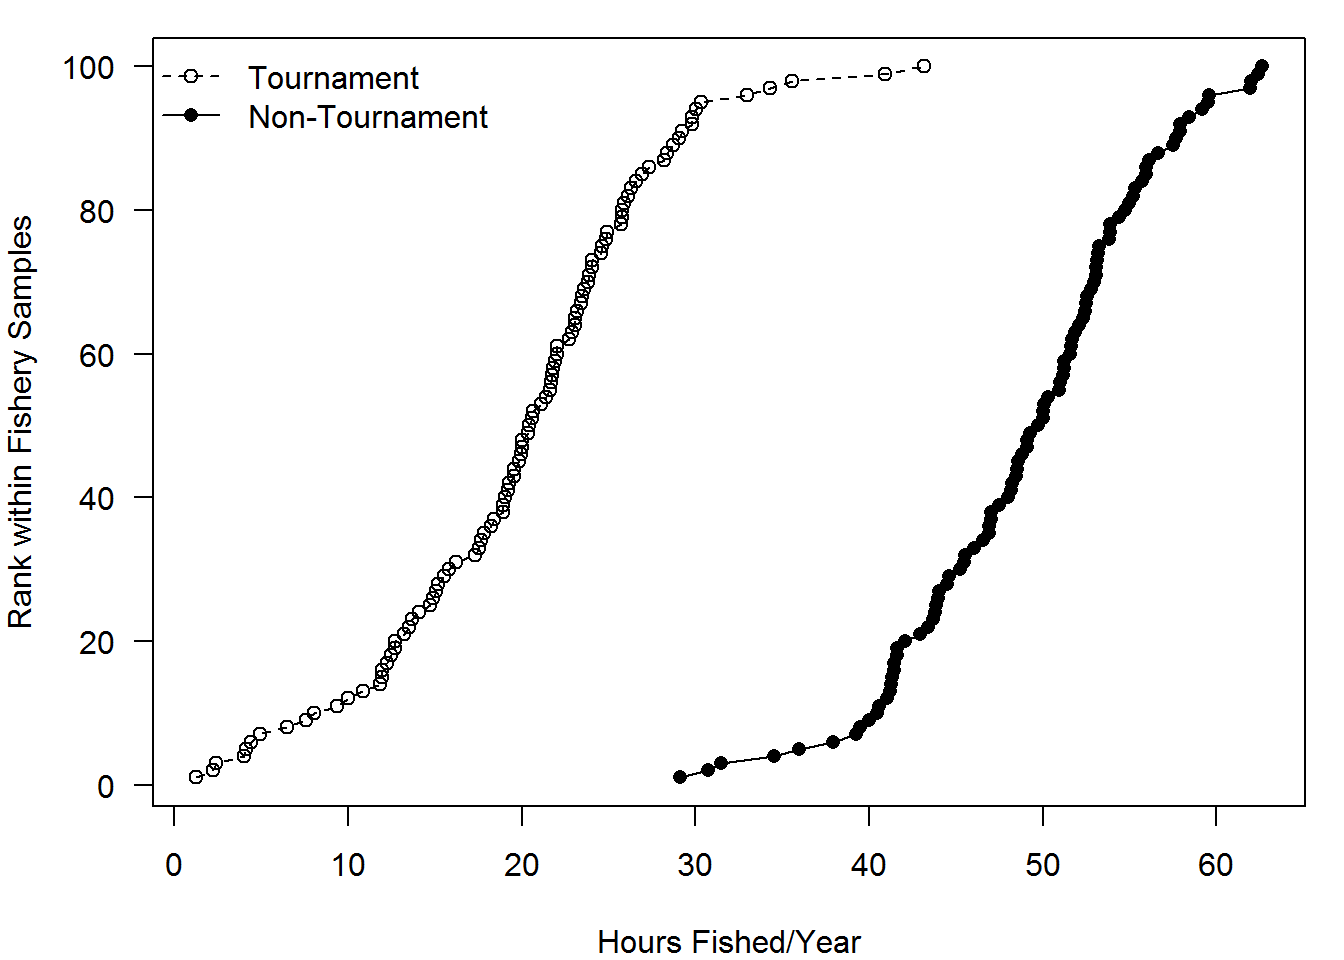
\includegraphics{au-r-workshop_files/figure-latex/unnamed-chunk-103-1} \end{center}

Notice four things:

\begin{enumerate}
\def\labelenumi{\arabic{enumi}.}
\tightlist
\item
  The use of \texttt{mp} to specify the \texttt{x} coordinates. If you
  do \texttt{mp\ =\ barplot(...)}, \texttt{mp} will contain the
  \texttt{x} coordinates of the midpoint of each bar.
\item
  \texttt{x0} and \texttt{x1} are the same: you wish to have vertical
  bars, so these must be the same while \texttt{y1} and \texttt{y2}
  differ.
\item
  The use of \texttt{ylim\ =\ range(c(0,\ upr))}: you want the y-axis to
  show the full range of all the error bars.
\item
  The three arguments at the end of \texttt{arrows}:

  \begin{itemize}
  \tightlist
  \item
    \texttt{length\ =\ 0.1}: the length of the arrow heads, fiddle with
    this until you like it.
  \item
    \texttt{angle\ =\ 90}: the angle of the arrow heads, you want 90
    here for the error bars.
  \item
    \texttt{code\ =\ 3}: indicates that arrow heads should be drawn on
    both ends of the arrow.
  \end{itemize}
\end{enumerate}

\begin{center}\rule{0.5\linewidth}{\linethickness}\end{center}

\hypertarget{ex2}{\section*{Exercise 2}\label{ex2}}
\addcontentsline{toc}{section}{Exercise 2}

For this exercise, you will be making a few of plots and changing how
they look to suit your taste. You will use a real dataset
(\texttt{sockeye.csv}, see the
\protect\hyperlink{data-sets}{instructions} regarding acquiring the data
files) this time from a sockeye salmon (\emph{Oncorhynchus nerka})
population from the Columbia/Snake River system, and the data set was
obtained from \citet{sockeye-cite}. This population spawns in Redfish
Lake in Idaho, which feeds into the Salmon River which is a tributary of
the Snake River. In order to reach the lake, the sockeye salmon must
successfully pass through a total eight dams that have fish passage
mechanisms in place. The Redfish Lake population is one of the most
endangered sockeye populations in the U.S. and travels farther (1,448
km), higher (1,996 m), and is the southernmost population of all sockeye
populations in the world \citep{sockeye-cite}. Given this uniqueness, a
captive breeding program was initiated in 1991 to conserve the genes
from this population. These data came from both hatchery-raised and wild
fish and include average female spawner weight (g), fecundity (number of
eggs), egg size (eggs/g), and \% survival to the eyed-egg stage.

\emph{The solutions to this exercise are found at the end of this book
(\protect\hyperlink{ex2-answers}{here}). You are \textbf{strongly
recommended} to make a good attempt at completing this exercise on your
own and only look at the solutions when you are truly stumped.}

\begin{enumerate}
\def\labelenumi{\arabic{enumi}.}
\tightlist
\item
  Create a new R script called \texttt{Ex2.R} and save it in the
  \texttt{Chapter2} directory. Read in the data set
  \texttt{sockeye.csv}. Produce a basic summary of the data and take
  note of the data classes, missing values (\texttt{NA}), and the
  relative ranges for each variable.
\item
  Make a histogram of fish weights for only hatchery-origin fish. Set
  \texttt{breaks\ =\ 10} so you can see the distribution more clearly.
\item
  Make a scatter plot of the fecundity of females as a function of their
  body weight for wild fish only. Use whichever plotting character
  (\texttt{pch}) and color (\texttt{col}) you wish. Change the main
  title and axes labels to reflect what they mean. Change the x-axis
  limits to be 600 to 3000 and the y-axis limits to be 0 to 3500.
  (\emph{Hint: The \texttt{NAs} will not cause a problem. R will only
  use points where there are paired records for both \texttt{x} and
  \texttt{y} and ignore otherwise}).
\item
  Add points that do the same thing but for hatchery fish. Use a
  different plotting character and a different color.
\item
  Add a legend to the plot to differentiate between the two types of
  fish.\\
\item
  Make a multi-panel plot in a new window with box-and-whisker plots
  that compare (1) spawner weight, (2) fecundity, and (3) egg size
  between hatchery and wild fish. (\emph{Hint: each comparison will be
  on its own panel}). Change the titles of each plot to reflect what you
  are comparing.
\item
  Save the plot as a .png file in your working directory with a file
  name of your choosing.
\end{enumerate}

\subsection*{EXERCISE 2 BONUS}\label{exercise-2-bonus}
\addcontentsline{toc}{subsection}{EXERCISE 2 BONUS}

\begin{enumerate}
\def\labelenumi{\arabic{enumi}.}
\tightlist
\item
  Make a bar plot comparing the mean survival to eyed-egg stage for each
  type of fish (hatchery and wild). Add error bars that represent 95\%
  confidence intervals.
\item
  Change the names of each bar, the main plot title, and the y-axis
  title.\\
\item
  Adjust the margins so there are 2 lines on the bottom, 5 on the left,
  2 on the top, and 1 on the right.
\end{enumerate}

\chapter{Basic Statistics}\label{ch3}

\section*{Chapter Overview}\label{chapter-overview-2}
\addcontentsline{toc}{section}{Chapter Overview}

In this chapter, you will get familiar with the basics of using R for
the purpose it was designed: statisitical analysis. You will learn how
to:

\begin{itemize}
\tightlist
\item
  fit and interpret the output from various general linear models:

  \begin{itemize}
  \tightlist
  \item
    simple linear regression models
  \item
    T-tests (also ANOVA)
  \item
    ANCOVA models
  \item
    Interactions
  \end{itemize}
\item
  conduct basic model selection
\item
  fit basic GLMs: the logistic regression model
\item
  Bonus topic: fitting non-linear regression models using \texttt{nls()}
\end{itemize}

R's built-in statistical modeling framework is pretty intuitive and
comprehensive. R has gained popularity as a statistics software and is
commonly used both in academia and governmental resource agencies. This
popularity is likely a result of its power, flexibility, intuitive
nature, and price (free!). For many students, this chapter may be the
one that is most immediately useful.

\textbf{IMPORTANT NOTE}: If you did not attend the sessions
corresponding to Chapters \ref{ch1} or \ref{ch2}, you are recommended to
walk through the material found in those chapters before proceeding to
this material. Also note that if you are confused about a topic, you can
use \textbf{CTRL + F} to find previous cases where that topic has been
discussed in this book.

\section*{Before You Begin}\label{before-you-begin-1}
\addcontentsline{toc}{section}{Before You Begin}

You should create a new directory and R script for your work in this
Chapter. Create a new R script called \texttt{Ch3.R} and save it in the
directory \texttt{C:/Users/YOU/Documents/R-Book/Chapter3}. Set your
working directory to that location. Revisit the material in Sections
\ref{scripts} and \ref{working-dir} for more details on these steps.

\section{The General Linear Model}\label{lm}

Much of this chapter will focus on the general linear model, so it is
important to become familiar with it. The general linear model is a
family of models that allows you to determine the relationship (if any)
between some continuous response variable (\(y\)) and some predictor
variable(s) (\(x_n\)) and is often written as:

\begin{equation}
  y_i=\beta_0 + \beta_1 x_{i1} + ... + \beta_j x_{ij}+ ... + \beta_n x_{in} + \varepsilon_i, \varepsilon_i \sim N(0,\sigma),
\label{eq:lin-mod}
\end{equation}

where the subscript \(i\) represents an individual observation. The
predictor variable(s) can be either categorical (i.e., grouping
variables used in ANOVA, t-test, etc.), continuous (regression), or a
combination of categorical and continuous (ANCOVA). The main focus is to
estimate the coefficients (\(\beta\)), and in some cases it is to
determine if their values are ``significantly'' different from the value
assumed by some null hypothesis.

The model makes several assumptions about the residuals\footnote{The
  residuals (\(\varepsilon_i\)) are the difference between the data
  point \(y_i\) and the model prediction \(\hat{y}_i\):
  \(\varepsilon_i=y_i-\hat{y}_i\)} to obtain estimates of the
coefficients. For reliable inference, the residuals must:

\begin{itemize}
\tightlist
\item
  be independent
\item
  be normally-distributed
\item
  have constant variance across range of the x-axis
\end{itemize}

In R, the general linear model is fitted using the \texttt{lm()}
function. Here's the basic syntax is
\texttt{lm(y\ \textasciitilde{}\ x,\ data\ =\ dat)}\footnote{This should
  look familar from Section \ref{box-whisker}}; it says: ``fit a model
with \texttt{y} as the response variable and \texttt{x} as the sole
predictor variable, look for the variables \texttt{x} and \texttt{y} in
a data frame called \texttt{dat}''.

\subsection{Simple Linear Regression}\label{regression}

Read the data found in \texttt{sockeye.csv} (see in the
\protect\hyperlink{data-sets}{instructions} for help with acquiring the
data) into R. This is the same data set you used in
\protect\hyperlink{ex2}{Exercise 2} - revisit this section for more
details on the meaning of the variables. These are real data and are
presented in \citet{sockeye-cite}.

\begin{Shaded}
\begin{Highlighting}[]
\NormalTok{dat =}\StringTok{ }\KeywordTok{read.csv}\NormalTok{(}\StringTok{"../Data/sockeye.csv"}\NormalTok{)}
\KeywordTok{head}\NormalTok{(dat)}
\end{Highlighting}
\end{Shaded}

\begin{verbatim}
##   year  type weight fecund egg_size survival
## 1 1991 hatch     NA     NA       NA       NA
## 2 1992 hatch     NA     NA       NA       NA
## 3 1993 hatch   1801   2182    12.25    46.58
## 4 1994 hatch   1681   2134     7.92    50.98
## 5 1995 hatch   2630   1576    21.61    68.06
## 6 1996 hatch   2165   2171     8.74    63.43
\end{verbatim}

To fit a regression model using \texttt{lm()}, both \texttt{x} and
\texttt{y} must be continous (numeric) variables. In the data set
\texttt{dat}, two such variables are the \texttt{weight} and
\texttt{fecund}. Fit a regression model where you link the average
fecundity (number of eggs) of an individual year to the average weight
(in grams) in that year. Ignore for now that the fish come from two
sources: hatchery and wild origin.

\begin{Shaded}
\begin{Highlighting}[]
\NormalTok{fit1 =}\StringTok{ }\KeywordTok{lm}\NormalTok{(fecund }\OperatorTok{~}\StringTok{ }\NormalTok{weight, }\DataTypeTok{data =}\NormalTok{ dat)}
\end{Highlighting}
\end{Shaded}

If you run just the \texttt{fit1} object, you will see the model you ran
along with the coefficient estimates of the intercept (\(\beta_0\)) and
the slope (\(\beta_1\)):

\begin{Shaded}
\begin{Highlighting}[]
\NormalTok{fit1}
\end{Highlighting}
\end{Shaded}

\begin{verbatim}
## 
## Call:
## lm(formula = fecund ~ weight, data = dat)
## 
## Coefficients:
## (Intercept)       weight  
##   1874.6496       0.2104
\end{verbatim}

This model looks like this:

\begin{equation}
  y_i=\beta_0 + \beta_1 x_{i1} + \varepsilon_i, \varepsilon_i \sim N(0,\sigma),
\label{eq:lin-reg}
\end{equation}

where \(x_{i1}\) is \texttt{weight}. The coefficients are interpretted
as:

\begin{itemize}
\tightlist
\item
  \(\beta_0\): the y-intercept (mean \texttt{fecund} at zero
  \texttt{weight})
\item
  \(\beta_1\): the slope (change in \texttt{fecund} for one unit
  increase in \texttt{weight})
\end{itemize}

For more information about the model fit, you can use the
\texttt{summary()} function:

\begin{Shaded}
\begin{Highlighting}[]
\KeywordTok{summary}\NormalTok{(fit1)}
\end{Highlighting}
\end{Shaded}

\begin{verbatim}
## 
## Call:
## lm(formula = fecund ~ weight, data = dat)
## 
## Residuals:
##     Min      1Q  Median      3Q     Max 
## -873.67 -389.28  -71.65  482.96 1041.24 
## 
## Coefficients:
##              Estimate Std. Error t value Pr(>|t|)    
## (Intercept) 1874.6496   269.4369   6.958 4.33e-08 ***
## weight         0.2104     0.1803   1.167    0.251    
## ---
## Signif. codes:  0 '***' 0.001 '**' 0.01 '*' 0.05 '.' 0.1 ' ' 1
## 
## Residual standard error: 500.6 on 35 degrees of freedom
##   (7 observations deleted due to missingness)
## Multiple R-squared:  0.03745,    Adjusted R-squared:  0.009945 
## F-statistic: 1.362 on 1 and 35 DF,  p-value: 0.2511
\end{verbatim}

Again the coefficient estimates are shown, but now you see the
uncertainty on the parameter estimates (standard errors), the test
statistic, and the p-value testing the null hypothesis that each
coefficient has a zero value. Here you can see that the p-value does not
support rejection of the null hypothesis that the slope is zero. You can
see the residual standard error (variability of data around the fitted
line and the estimate of \(\sigma\)), the \(R^2\) value (the proportion
of variation in \texttt{fecund} explained by variation in
\texttt{weight}), and the p-value of the overall model.

You can easily see the model fit by using the \texttt{abline()}
function. Make a new plot and add the fitted regression line:

\begin{Shaded}
\begin{Highlighting}[]
\KeywordTok{plot}\NormalTok{(fecund }\OperatorTok{~}\StringTok{ }\NormalTok{weight, }\DataTypeTok{data =}\NormalTok{ dat, }\DataTypeTok{col =} \StringTok{"grey"}\NormalTok{, }\DataTypeTok{pch =} \DecValTok{16}\NormalTok{, }\DataTypeTok{cex =} \FloatTok{1.5}\NormalTok{)}
\KeywordTok{abline}\NormalTok{(fit1)}
\end{Highlighting}
\end{Shaded}

\begin{center}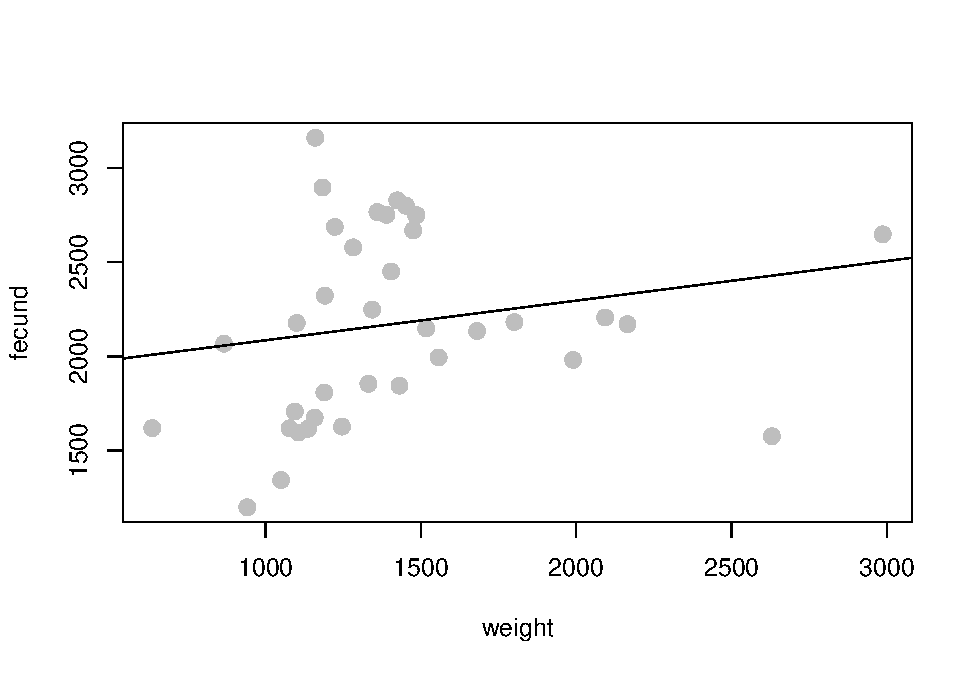
\includegraphics{au-r-workshop_files/figure-latex/unnamed-chunk-111-1} \end{center}

It fits, but not very well. It seems there are two groups: one with data
points mostly above the line and one with data points mostly below the
line. You'll now run a new model to get at this.

\subsection{ANOVA: Categorical predictors}\label{anova}

ANOVA models attempt to determine if the means of different groups are
different. You can fit them in the same basic \texttt{lm()} framework.
But first, notice that:

\begin{Shaded}
\begin{Highlighting}[]
\KeywordTok{class}\NormalTok{(dat}\OperatorTok{$}\NormalTok{type); }\KeywordTok{levels}\NormalTok{(dat}\OperatorTok{$}\NormalTok{type)}
\end{Highlighting}
\end{Shaded}

\begin{verbatim}
## [1] "factor"
\end{verbatim}

\begin{verbatim}
## [1] "hatch" "wild"
\end{verbatim}

tells you the \texttt{type} variable is a factor. It has levels of
\texttt{"hatch"} and \texttt{"wild"} which indicate the origin of the
adult spawning fish sampled each year. If you pass \texttt{lm()} a
predictor variable with a factor class, R will automatically fit it as
an ANOVA model. See Section \ref{factors} for more details on factors.
Factors have an explicit ordering of the levels. By default, this
ordering happens alphabetically: if your factor has levels \texttt{"a"},
\texttt{"b"}, and \texttt{"c"}, they will be assigned the order of
\texttt{1}, \texttt{2} and \texttt{3}, respectively. You can always see
how R is ordering your factor by doing something similar to this:

\begin{Shaded}
\begin{Highlighting}[]
\NormalTok{pairs =}\StringTok{ }\KeywordTok{cbind}\NormalTok{(}
  \KeywordTok{as.character}\NormalTok{(dat}\OperatorTok{$}\NormalTok{type),}
  \KeywordTok{as.numeric}\NormalTok{(dat}\OperatorTok{$}\NormalTok{type)}
\NormalTok{)}

\KeywordTok{head}\NormalTok{(pairs); }\KeywordTok{tail}\NormalTok{(pairs)}
\end{Highlighting}
\end{Shaded}

\begin{verbatim}
##      [,1]    [,2]
## [1,] "hatch" "1" 
## [2,] "hatch" "1" 
## [3,] "hatch" "1" 
## [4,] "hatch" "1" 
## [5,] "hatch" "1" 
## [6,] "hatch" "1"
\end{verbatim}

\begin{verbatim}
##       [,1]   [,2]
## [39,] "wild" "2" 
## [40,] "wild" "2" 
## [41,] "wild" "2" 
## [42,] "wild" "2" 
## [43,] "wild" "2" 
## [44,] "wild" "2"
\end{verbatim}

The functions \texttt{as.character} and \texttt{as.numeric} are coersion
functions: they attempt to change the way something is interpretted.
Notice that the level \texttt{"hatch"} is assigned the order \texttt{1}
because it comes before \texttt{"wild"} alphebetically. The first level
is termed the \textbf{reference level} because it is the group that all
other levels are compared to when fitting a model. You can change the
reference level using
\texttt{dat\$type\_rlvl\ =\ relevel(dat\$type,\ ref\ =\ "wild")}.

You are now ready to fit the ANOVA model, which will measure the size of
the difference in the mean \texttt{fecund} between different levels of
the factor \texttt{type}:

\begin{Shaded}
\begin{Highlighting}[]
\NormalTok{fit2 =}\StringTok{ }\KeywordTok{lm}\NormalTok{(fecund }\OperatorTok{~}\StringTok{ }\NormalTok{type, }\DataTypeTok{data =}\NormalTok{ dat)}
\end{Highlighting}
\end{Shaded}

Think of this model as being written as:

\begin{equation}
  y_i=\beta_0 + \beta_1 x_{i1} + \varepsilon_i
\label{eq:anova}
\end{equation}

and assume that \(x_{i1} = 0\) if observation \(i\) is a fish from the
\texttt{"hatch"} level and \(x_{i1} = 1\) if observation \(i\) is a fish
from the \texttt{"wild"} level. Note that Equations \eqref{eq:lin-reg} and
\eqref{eq:anova} are the same, the only thing that differs is the coding
of the variable \(x_{i1}\). In the ANOVA case:

\begin{itemize}
\tightlist
\item
  \(\beta_0\) (the intercept) is the mean \texttt{fecund} for the
  \texttt{"hatch"} level and
\item
  \(\beta_1\) is the difference in mean \texttt{fecund}: \texttt{"wild"}
  - \texttt{"hatch"}.
\end{itemize}

So when you run \texttt{coef(fit2)} to extract the coefficient estimates
and get:

\begin{verbatim}
## (Intercept)    typewild 
##   1846.2500    713.3971
\end{verbatim}

you see that the mean fecundity of hatchery fish is about 1846 eggs and
that the average wild fish has about 713 more eggs than the average
hatchery fish across all years. The fact that the p-value associated
with the \texttt{typewild} coefficient when you run
\texttt{summary(fit2)} is less than 0.05 indicates that there is
statistical evidence that the difference in means is not zero.

Verify your interpretation of the coefficients:

\begin{Shaded}
\begin{Highlighting}[]
\NormalTok{m =}\StringTok{ }\KeywordTok{tapply}\NormalTok{(dat}\OperatorTok{$}\NormalTok{fecund, dat}\OperatorTok{$}\NormalTok{type, mean, }\DataTypeTok{na.rm =}\NormalTok{ T)}

\CommentTok{# b0:}
\NormalTok{m[}\DecValTok{1}\NormalTok{]}
\end{Highlighting}
\end{Shaded}

\begin{verbatim}
##   hatch 
## 1846.25
\end{verbatim}

\begin{Shaded}
\begin{Highlighting}[]
\CommentTok{# b1:}
\NormalTok{m[}\DecValTok{2}\NormalTok{] }\OperatorTok{-}\StringTok{ }\NormalTok{m[}\DecValTok{1}\NormalTok{]}
\end{Highlighting}
\end{Shaded}

\begin{verbatim}
##     wild 
## 713.3971
\end{verbatim}

\subsection{ANCOVA: Continuous and categorical
predictors}\label{ancova-continuous-and-categorical-predictors}

Now that you have seen that hatchery and wild fish tend to separate
along the fecundity axis (as evidenced by the ANOVA results above), you
would like to include this in your original regression model. You will
fit two regression lines within the same model: one for hatchery fish
and one for wild fish. This model is called an ANCOVA model and looks
like this:

\begin{equation}
  y_i=\beta_0 + \beta_1 x_{i1} + \beta_2 x_{i2} + \varepsilon_i
\label{eq:ancova}
\end{equation}

If \(x_{i1}\) is \texttt{type} coded with 0's and 1's as in Section
\ref{anova} and \(x_{i2}\) is \texttt{weight}, then the coefficients are
interpretted as:

\begin{itemize}
\tightlist
\item
  \(\beta_0\): the y-intercept of the \texttt{"hatch"} level (the
  reference level)
\item
  \(\beta_1\): the difference in mean \texttt{fecund} at the same
  weight: \texttt{"wild"} - \texttt{"hatch"}
\item
  \(\beta_2\): the slope of the \texttt{fecund} \emph{vs.}
  \texttt{weight} relationship (this model assumes the lines have common
  slopes, i.e., that the lines are parallel)
\end{itemize}

You can fit this model and extract the coefficents table from the
summary:

\begin{Shaded}
\begin{Highlighting}[]
\NormalTok{fit3 =}\StringTok{ }\KeywordTok{lm}\NormalTok{(fecund }\OperatorTok{~}\StringTok{ }\NormalTok{type }\OperatorTok{+}\StringTok{ }\NormalTok{weight, }\DataTypeTok{data =}\NormalTok{ dat)}
\KeywordTok{summary}\NormalTok{(fit3)}\OperatorTok{$}\NormalTok{coef}
\end{Highlighting}
\end{Shaded}

\begin{verbatim}
##                 Estimate  Std. Error  t value     Pr(>|t|)
## (Intercept) 1039.6417645 175.0992184 5.937444 1.038268e-06
## typewild     866.9909998  96.2473387 9.007948 1.578239e-10
## weight         0.5173716   0.1051039 4.922477 2.164460e-05
\end{verbatim}

And you can plot the fit. Study this code to make sure you know what
each is doing. Use what you know about the meanings of the three
coefficients to decipher the two \texttt{abline()} commands. Remember
that \texttt{abline()} takes takes two arguments: \texttt{a} is the
intercept and \texttt{b} is the slope.

\begin{Shaded}
\begin{Highlighting}[]
\KeywordTok{plot}\NormalTok{(fecund }\OperatorTok{~}\StringTok{ }\NormalTok{weight, }\DataTypeTok{data =}\NormalTok{ dat, }\DataTypeTok{col =} \StringTok{"grey"}\NormalTok{,}
     \DataTypeTok{pch =} \KeywordTok{ifelse}\NormalTok{(dat}\OperatorTok{$}\NormalTok{type }\OperatorTok{==}\StringTok{ "hatch"}\NormalTok{, }\DecValTok{1}\NormalTok{, }\DecValTok{16}\NormalTok{), }\DataTypeTok{cex =} \FloatTok{1.5}\NormalTok{)}
\KeywordTok{abline}\NormalTok{(}\KeywordTok{coef}\NormalTok{(fit3)[}\KeywordTok{c}\NormalTok{(}\DecValTok{1}\NormalTok{,}\DecValTok{3}\NormalTok{)], }\DataTypeTok{lty =} \DecValTok{2}\NormalTok{)}
\KeywordTok{abline}\NormalTok{(}\KeywordTok{sum}\NormalTok{(}\KeywordTok{coef}\NormalTok{(fit3)[}\KeywordTok{c}\NormalTok{(}\DecValTok{1}\NormalTok{,}\DecValTok{2}\NormalTok{)]), }\KeywordTok{coef}\NormalTok{(fit3)[}\DecValTok{3}\NormalTok{])}
\KeywordTok{legend}\NormalTok{(}\StringTok{"bottom"}\NormalTok{, }\DataTypeTok{legend =} \KeywordTok{c}\NormalTok{(}\StringTok{"Hatchery"}\NormalTok{, }\StringTok{"Wild"}\NormalTok{), }\DataTypeTok{pch =} \KeywordTok{c}\NormalTok{(}\DecValTok{1}\NormalTok{,}\DecValTok{16}\NormalTok{), }\DataTypeTok{lty =} \KeywordTok{c}\NormalTok{(}\DecValTok{2}\NormalTok{,}\DecValTok{1}\NormalTok{),}
       \DataTypeTok{col =} \StringTok{"grey"}\NormalTok{, }\DataTypeTok{pt.cex =} \FloatTok{1.5}\NormalTok{, }\DataTypeTok{bty =} \StringTok{"n"}\NormalTok{, }\DataTypeTok{horiz =}\NormalTok{ T)}
\end{Highlighting}
\end{Shaded}

\begin{center}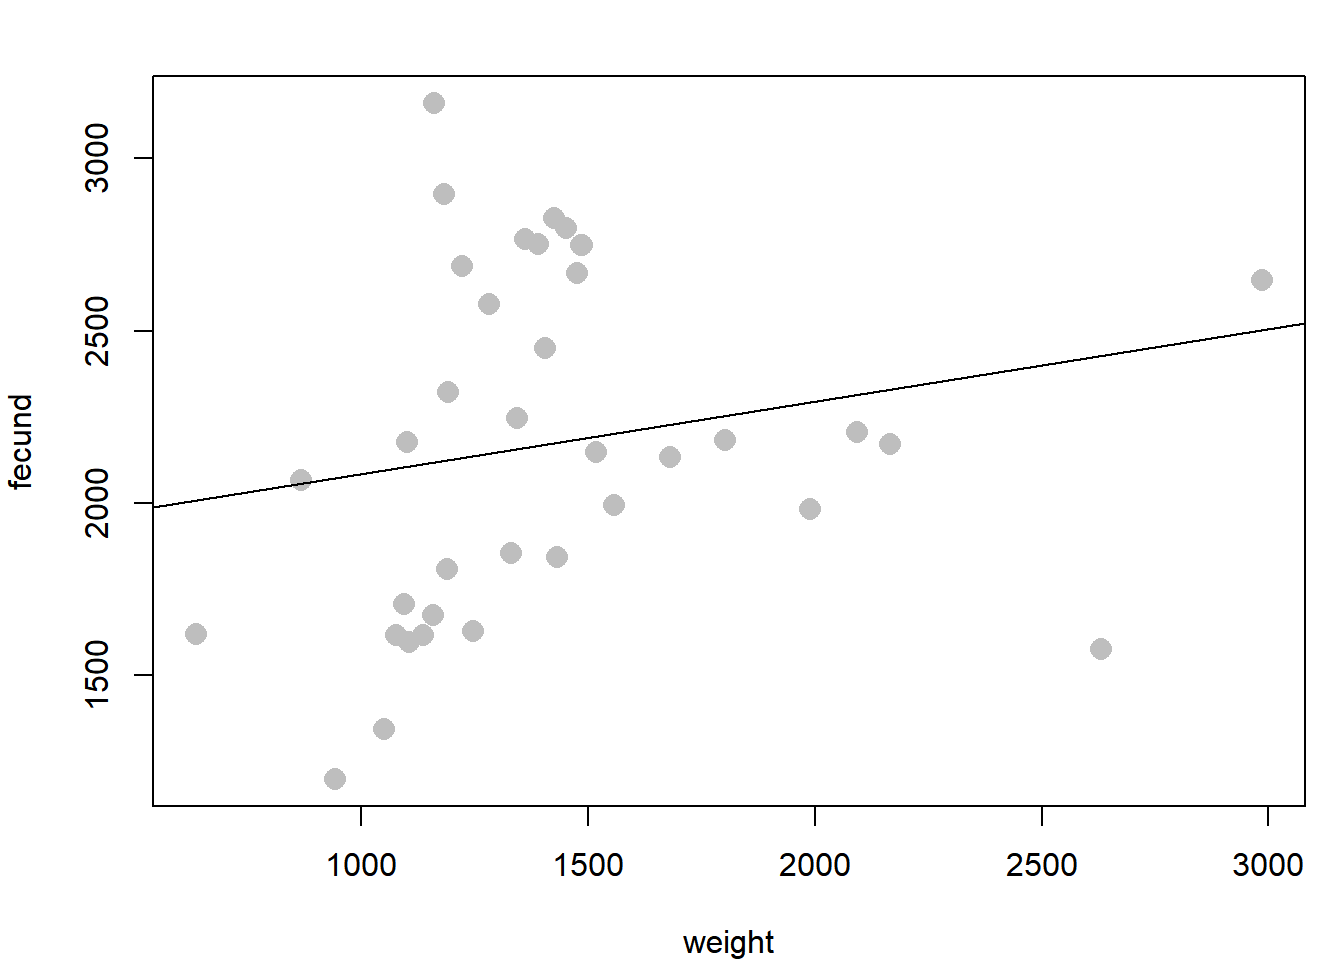
\includegraphics{au-r-workshop_files/figure-latex/unnamed-chunk-118-1} \end{center}

\subsection{Interactions}\label{interactions}

Above, you have included an additional predictor variable (and
parameter) in your model to help explain variation in the
\texttt{fecund} variable. However, you have assumed that the effect of
weight on fecundity is common between hatchery and wild fish (note the
parallel lines in the figure above). You may have reason to believe that
the effect of weight depends on the origin of the fish, e.g., wild fish
may tend to accumulate more eggs than hatchery fish for the same
increase in weight. Cases where the magnitude of the effect depends on
the value of another predictor variable are known as ``interactions''.
You can write the interactive ANCOVA model like this:

\begin{equation}
  y_i=\beta_0 + \beta_1 x_{i1} + \beta_2 x_{i2} + \beta_3 x_{i1} x_{i2} + \varepsilon_i
\label{eq:ancova-interact}
\end{equation}

If \(x_{i1}\) is \texttt{type} coded with 0's and 1's as in Section
\ref{anova} and \(x_{i2}\) is \texttt{weight}, then the coefficients are
interpretted as:

\begin{itemize}
\tightlist
\item
  \(\beta_0\): the y-intercept of the \texttt{"hatch"} level (the
  reference level)
\item
  \(\beta_1\): the difference in y-intercept between the \texttt{"wild"}
  level and the \texttt{"hatch"} level.
\item
  \(\beta_2\): the slope of the \texttt{"hatch"} level
\item
  \(\beta_3\): the difference in slope between the \texttt{"wild"} level
  and the \texttt{"hatch"} level.
\end{itemize}

You can fit this model:

\begin{Shaded}
\begin{Highlighting}[]
\NormalTok{fit4 =}\StringTok{ }\KeywordTok{lm}\NormalTok{(fecund }\OperatorTok{~}\StringTok{ }\NormalTok{type }\OperatorTok{+}\StringTok{ }\NormalTok{weight }\OperatorTok{+}\StringTok{ }\NormalTok{type}\OperatorTok{:}\NormalTok{weight, }\DataTypeTok{data =}\NormalTok{ dat)}

\CommentTok{# or}
\CommentTok{# fit4 = lm(fecund ~ type * weight, data = dat)}
\end{Highlighting}
\end{Shaded}

The first option above is more clear in its statement, but both do the
same thing.

Plot the fit. Study these lines to make sure you know what each is
doing. Use what you know about the meanings of the four coefficients to
decipher the two \texttt{abline()} commands.

\begin{Shaded}
\begin{Highlighting}[]
\KeywordTok{plot}\NormalTok{(fecund }\OperatorTok{~}\StringTok{ }\NormalTok{weight, }\DataTypeTok{data =}\NormalTok{ dat, }\DataTypeTok{col =} \StringTok{"grey"}\NormalTok{,}
     \DataTypeTok{pch =} \KeywordTok{ifelse}\NormalTok{(dat}\OperatorTok{$}\NormalTok{type }\OperatorTok{==}\StringTok{ "hatch"}\NormalTok{, }\DecValTok{1}\NormalTok{, }\DecValTok{16}\NormalTok{), }\DataTypeTok{cex =} \FloatTok{1.5}\NormalTok{)}
\KeywordTok{abline}\NormalTok{(}\KeywordTok{coef}\NormalTok{(fit4)[}\KeywordTok{c}\NormalTok{(}\DecValTok{1}\NormalTok{,}\DecValTok{3}\NormalTok{)], }\DataTypeTok{lty =} \DecValTok{2}\NormalTok{)}
\KeywordTok{abline}\NormalTok{(}\KeywordTok{sum}\NormalTok{(}\KeywordTok{coef}\NormalTok{(fit4)[}\KeywordTok{c}\NormalTok{(}\DecValTok{1}\NormalTok{,}\DecValTok{2}\NormalTok{)]), }\KeywordTok{sum}\NormalTok{(}\KeywordTok{coef}\NormalTok{(fit4)[}\KeywordTok{c}\NormalTok{(}\DecValTok{3}\NormalTok{,}\DecValTok{4}\NormalTok{)]))}
\KeywordTok{legend}\NormalTok{(}\StringTok{"bottom"}\NormalTok{, }\DataTypeTok{legend =} \KeywordTok{c}\NormalTok{(}\StringTok{"Hatchery"}\NormalTok{, }\StringTok{"Wild"}\NormalTok{), }\DataTypeTok{pch =} \KeywordTok{c}\NormalTok{(}\DecValTok{1}\NormalTok{,}\DecValTok{16}\NormalTok{), }\DataTypeTok{lty =} \KeywordTok{c}\NormalTok{(}\DecValTok{2}\NormalTok{,}\DecValTok{1}\NormalTok{),}
       \DataTypeTok{col =} \StringTok{"grey"}\NormalTok{, }\DataTypeTok{pt.cex =} \FloatTok{1.5}\NormalTok{, }\DataTypeTok{bty =} \StringTok{"n"}\NormalTok{, }\DataTypeTok{horiz =}\NormalTok{ T)}
\end{Highlighting}
\end{Shaded}

\begin{center}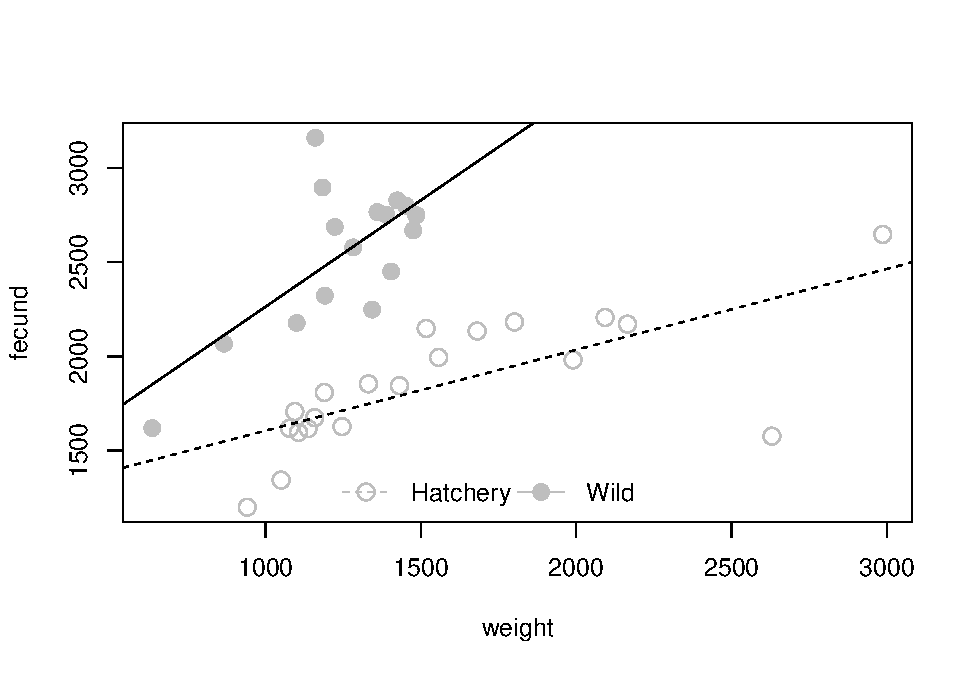
\includegraphics{au-r-workshop_files/figure-latex/unnamed-chunk-120-1} \end{center}

Based on the coefficients table:

\begin{Shaded}
\begin{Highlighting}[]
\KeywordTok{summary}\NormalTok{(fit4)}\OperatorTok{$}\NormalTok{coef}
\end{Highlighting}
\end{Shaded}

\begin{verbatim}
##                     Estimate Std. Error    t value     Pr(>|t|)
## (Intercept)     1175.7190847 174.545223  6.7358995 1.125255e-07
## typewild         -42.8721082 398.980751 -0.1074541 9.150794e-01
## weight             0.4300894   0.105592  4.0731253 2.732580e-04
## typewild:weight    0.7003389   0.299104  2.3414560 2.539681e-02
\end{verbatim}

It seems that fish of the different origins have approximately the same
intercept, but that their slopes are quite different.

\subsection{AIC Model Selection}\label{aic-model-selection}

You have now fitted four different models, each that makes different
claims about how you can predict the fecundity of a given sockeye salmon
at Redfish Lake. If you are interested in determining \emph{which} of
these models you should use for prediction, you need to use
\textbf{model selection}. Model selection attempts to find the model
that is likely to have the smallest out-of-sample prediction error
(i.e., future predictions will be close to what actually happens). One
model selection metric is the AIC\footnote{Akaike's Information
  Criterion. An excellent overview of AIC with ecological applications
  is given in \citet{aic-cite}}. Lower AIC values mean the model should
have better predictive performance. Obtain a simple AIC table from your
fitted model objects and sort the table by increasing values of AIC:

\begin{Shaded}
\begin{Highlighting}[]
\NormalTok{tab =}\StringTok{ }\KeywordTok{AIC}\NormalTok{(fit1, fit2, fit3, fit4)}
\NormalTok{tab[}\KeywordTok{order}\NormalTok{(tab}\OperatorTok{$}\NormalTok{AIC),]}
\end{Highlighting}
\end{Shaded}

\begin{verbatim}
##      df      AIC
## fit4  5 522.0968
## fit3  4 525.7834
## fit2  3 543.6914
## fit1  3 568.9166
\end{verbatim}

In general, AIC values that are different by more than 2 units are
interpretted as having importantly different predictive performance.
Based on this very quick-and-dirty analysis, it seems that in predicting
future fecundity, you would want to use the interactive ANCOVA model.

\section{The Generalized Linear Model}\label{glms}

The models you fitted above were called ``general linear models''. They
all made the assumption that the residuals (\(\varepsilon_i\)) are
normally-distributed and that the response variable and the predictor
variables are linearly related. Oftentimes data and analyses do not
follow this assumption. For these cases you should often move to the
broader family of statistical models known as \textbf{generalized linear
models}\footnote{General linear models are a member of this family}.

\subsection{Logistic Regression}\label{logis-regression}

One example is in the case of \textbf{binary} data. Binary data have two
outcomes, e.g., success/failure, lived/died, male/female,
spawned/gravid, happy/sad, etc. If you wish to predict how the
probability of one outcome over the other changes depending on some
other variable, then you need to use the \textbf{logistic regression
model}, which is written as:

\begin{equation}
  logit(p_i)=\beta_0 + \beta_1 x_{i1} + ... + \beta_j x_{ij}+ ... + \beta_n x_{in}, y_i \sim Bernoulli(p_i)
\label{eq:logis-reg}
\end{equation}

Where \(p_i\) is the probability of success for trial \(i\)
(\(y_i = 1\)) at the values of the predictor variables \(x_{ij}\). The
\(logit(p_i)\) is the \textbf{link function} that links the linear
parameter scale to the data scale. It constrains the value of \(p_i\) to
be between 0 and 1 regardless of the values of the \(\beta\)
coefficients. The logit link function does this:

\begin{equation}
  logit(p_i) = log\left(\frac{p_i}{1-p_i}\right)
\label{eq:logit}
\end{equation}

which is the natural logarithm of the \textbf{odds}, a measure of how
likely the event is to happen relative to it not happening. Make an R
function to calculate the logit transformation:

\begin{Shaded}
\begin{Highlighting}[]
\NormalTok{logit =}\StringTok{ }\ControlFlowTok{function}\NormalTok{(p) \{}
  \KeywordTok{log}\NormalTok{(p}\OperatorTok{/}\NormalTok{(}\DecValTok{1} \OperatorTok{-}\StringTok{ }\NormalTok{p))}
\NormalTok{\}}
\end{Highlighting}
\end{Shaded}

If you have the result of \texttt{logit(p{[}i{]})} (which is given by
the \(\beta\) coefficients and the \(x_{ij}\) data in Equation
\eqref{eq:logis-reg}) and need to get \texttt{p{[}i{]}}, you can apply the
inverse logit function:

\begin{equation}
  expit(lp_i)=\frac{e^{lp_i}}{1 + e^{lp_i}}
\label{eq:expit}
\end{equation}

where \(lp_i = logit(p_i)\). Make a function for the inverse logit
transformation:

\begin{Shaded}
\begin{Highlighting}[]
\NormalTok{expit =}\StringTok{ }\ControlFlowTok{function}\NormalTok{(lp) \{  }\CommentTok{# lp stands for logit(p)}
  \KeywordTok{exp}\NormalTok{(lp)}\OperatorTok{/}\NormalTok{(}\DecValTok{1} \OperatorTok{+}\StringTok{ }\KeywordTok{exp}\NormalTok{(lp))}
\NormalTok{\}}
\end{Highlighting}
\end{Shaded}

Because of the logit link function, the coefficients have different
interpretations than in the general linear models you fitted in the
previous section: they are expressed in terms of \textbf{log odds}.

Fit a logistic regression model to the sockeye salmon data. None of the
variables of interest are binary, but you can create one. Look at the
variable \texttt{dat\$survival}. This is the average \% survival of all
eggs laid that make it to the ``eye-egg'' stage. Create a new variable
\texttt{binary} which takes on a 0 if \texttt{dat\$survival} is less
than 70\% and a 1 otherwise:

\begin{Shaded}
\begin{Highlighting}[]
\NormalTok{dat}\OperatorTok{$}\NormalTok{binary =}\StringTok{ }\KeywordTok{ifelse}\NormalTok{(dat}\OperatorTok{$}\NormalTok{survival }\OperatorTok{<}\StringTok{ }\DecValTok{70}\NormalTok{, }\DecValTok{0}\NormalTok{, }\DecValTok{1}\NormalTok{)}
\end{Highlighting}
\end{Shaded}

This will be your response variable and your model will estimate how the
probability of \texttt{binary} being a \texttt{1} changes (or doesn't)
depending on the value of other variables.

Analogous to the simple linear regression model (Section
\ref{regression}), estimate how \(p\) changes with \texttt{weight}:

\begin{Shaded}
\begin{Highlighting}[]
\NormalTok{fit1 =}\StringTok{ }\KeywordTok{glm}\NormalTok{(binary }\OperatorTok{~}\StringTok{ }\NormalTok{weight, }\DataTypeTok{data =}\NormalTok{ dat, }\DataTypeTok{family =}\NormalTok{ binomial)}
\KeywordTok{summary}\NormalTok{(fit1)}\OperatorTok{$}\NormalTok{coef}
\end{Highlighting}
\end{Shaded}

\begin{verbatim}
##                 Estimate Std. Error   z value   Pr(>|z|)
## (Intercept)  4.363441330 1.76943946  2.466002 0.01366306
## weight      -0.002819271 0.00125243 -2.251040 0.02438303
\end{verbatim}

The coefficients are interpretted as (remember, ``success'' is defined
as having at least 70\% egg survival to the stage of interest):

\begin{itemize}
\tightlist
\item
  \(\beta_0\): the log odds of success for a fish with zero weight
  (which is not all that important, let alone difficult to interpret).
  It can be transformed into more interpretable quantities:

  \begin{itemize}
  \tightlist
  \item
    \(e^{\beta_0}\) is the odds of success for fish with zero weight and
  \item
    \(expit(e^{\beta_0})\) is the probability of success for fish with
    zero weight.
  \end{itemize}
\item
  \(\beta_1\): the additive effect of fish weight on the log odds of
  success. More interpretable expressions are:

  \begin{itemize}
  \tightlist
  \item
    \(e^{\beta_1}\) is the ratio of the odds of success at two
    consective weights (e.g., 1500 and 1501) and Claims about
    \(e^{\beta_1}\) are made as ``for every one gram increase in weight,
    success became * \(e^{\beta_1}\) times as likely to happen''.
  \end{itemize}
\item
  You can predict the probability of success at any weight using
  \(expit(\beta_0 + \beta_1 weight)\)
\end{itemize}

You can plot the fitted model:

\begin{Shaded}
\begin{Highlighting}[]
\CommentTok{# create a sequence of weights to predict at}
\NormalTok{wt_seq =}\StringTok{ }\KeywordTok{seq}\NormalTok{(}\KeywordTok{min}\NormalTok{(dat}\OperatorTok{$}\NormalTok{weight, }\DataTypeTok{na.rm =}\NormalTok{ T),}
             \KeywordTok{max}\NormalTok{(dat}\OperatorTok{$}\NormalTok{weight, }\DataTypeTok{na.rm =}\NormalTok{ t),}
             \DataTypeTok{length =} \DecValTok{100}\NormalTok{)}

\CommentTok{# extract the coefficients and get p}
\NormalTok{p =}\StringTok{ }\KeywordTok{expit}\NormalTok{(}\KeywordTok{coef}\NormalTok{(fit1)[}\DecValTok{1}\NormalTok{] }\OperatorTok{+}\StringTok{ }\KeywordTok{coef}\NormalTok{(fit1)[}\DecValTok{2}\NormalTok{] }\OperatorTok{*}\StringTok{ }\NormalTok{wt_seq)}

\CommentTok{# plot the relationship}
\KeywordTok{plot}\NormalTok{(p }\OperatorTok{~}\StringTok{ }\NormalTok{wt_seq, }\DataTypeTok{type =} \StringTok{"l"}\NormalTok{, }\DataTypeTok{lwd =} \DecValTok{3}\NormalTok{, }\DataTypeTok{ylim =} \KeywordTok{c}\NormalTok{(}\DecValTok{0}\NormalTok{,}\DecValTok{1}\NormalTok{), }\DataTypeTok{las =} \DecValTok{1}\NormalTok{)}
\end{Highlighting}
\end{Shaded}

\begin{center}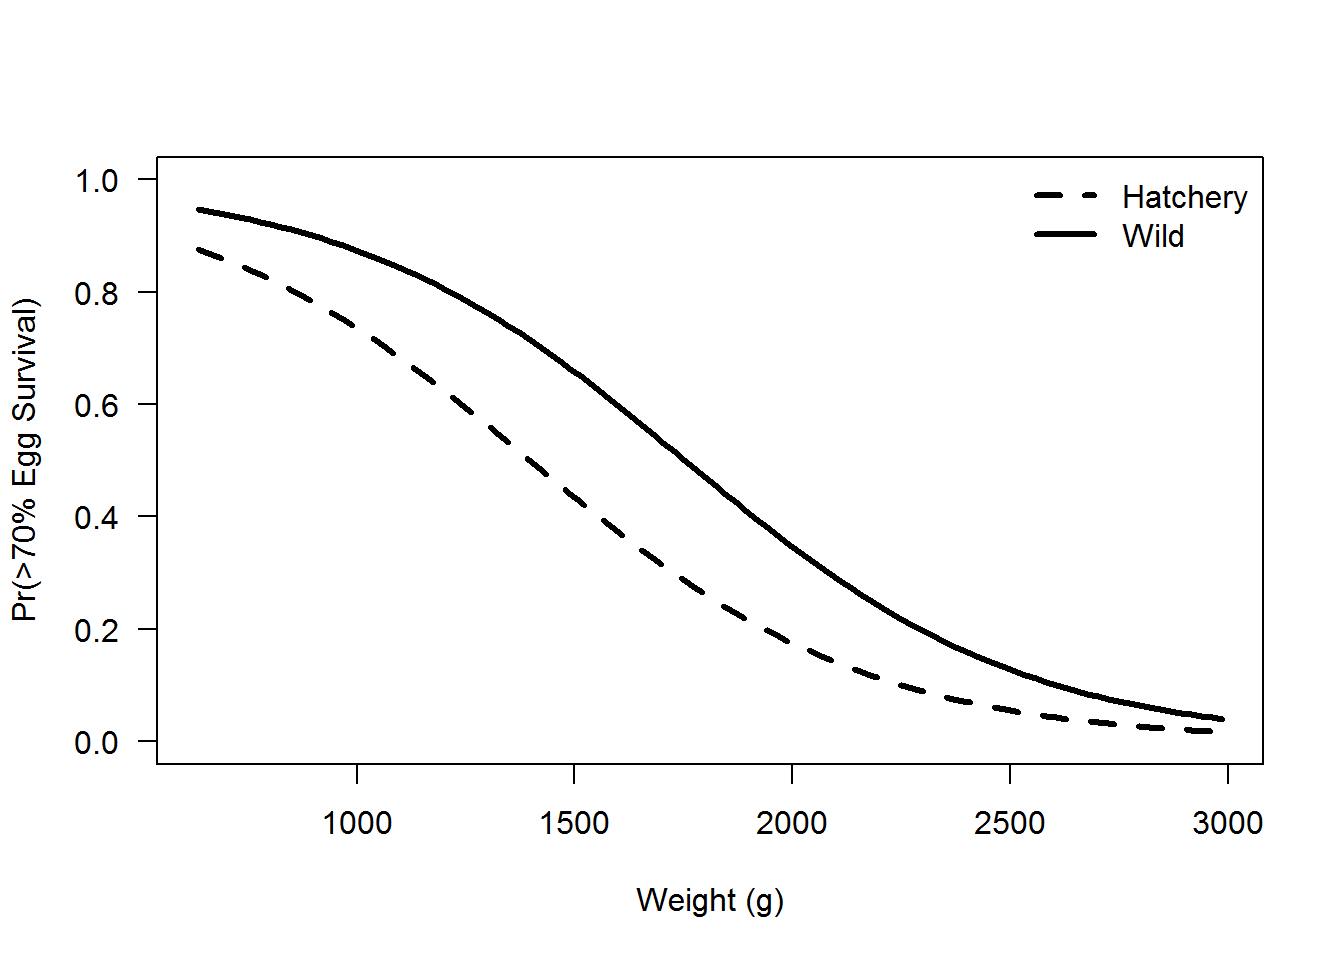
\includegraphics{au-r-workshop_files/figure-latex/unnamed-chunk-127-1} \end{center}

Fit another model comparing the probability of success between hatchery
and wild fish (analogous to the ANOVA model in Section \ref{anova}):

\begin{Shaded}
\begin{Highlighting}[]
\NormalTok{fit2 =}\StringTok{ }\KeywordTok{glm}\NormalTok{(binary }\OperatorTok{~}\StringTok{ }\NormalTok{type, }\DataTypeTok{data =}\NormalTok{ dat, }\DataTypeTok{family =}\NormalTok{ binomial)}
\KeywordTok{summary}\NormalTok{(fit2)}\OperatorTok{$}\NormalTok{coef}
\end{Highlighting}
\end{Shaded}

\begin{verbatim}
##               Estimate Std. Error    z value  Pr(>|z|)
## (Intercept) -0.2006707  0.4494666 -0.4464641 0.6552620
## typewild     1.3793257  0.7272845  1.8965421 0.0578884
\end{verbatim}

An easier way to obtain the predicted probability is by using the
\texttt{predict} function:

\begin{Shaded}
\begin{Highlighting}[]
\KeywordTok{predict}\NormalTok{(fit2,}
        \DataTypeTok{newdata =} \KeywordTok{data.frame}\NormalTok{(}\DataTypeTok{type =} \KeywordTok{c}\NormalTok{(}\StringTok{"hatch"}\NormalTok{, }\StringTok{"wild"}\NormalTok{)),}
        \DataTypeTok{type =} \StringTok{"response"}\NormalTok{)}
\end{Highlighting}
\end{Shaded}

\begin{verbatim}
##         1         2 
## 0.4500000 0.7647059
\end{verbatim}

This plugs in the two possible values of the predictor variable and asks
for the fitted probabilities.

Incorporate the origin type into your original model:

\begin{Shaded}
\begin{Highlighting}[]
\NormalTok{fit3 =}\StringTok{ }\KeywordTok{glm}\NormalTok{(binary }\OperatorTok{~}\StringTok{ }\NormalTok{type }\OperatorTok{+}\StringTok{ }\NormalTok{weight, }\DataTypeTok{data =}\NormalTok{ dat)}
\end{Highlighting}
\end{Shaded}

and obtain/plot the fitted probabilities for each group:

\begin{Shaded}
\begin{Highlighting}[]
\NormalTok{p_hatch =}\StringTok{ }\KeywordTok{predict}\NormalTok{(}
\NormalTok{  fit3, }\DataTypeTok{newdata =} \KeywordTok{data.frame}\NormalTok{(}\DataTypeTok{type =} \StringTok{"hatch"}\NormalTok{, }\DataTypeTok{weight =}\NormalTok{ wt_seq),}
  \DataTypeTok{type =} \StringTok{"response"}
\NormalTok{)}
\NormalTok{p_wild =}\StringTok{ }\KeywordTok{predict}\NormalTok{(}
\NormalTok{  fit3, }\DataTypeTok{newdata =} \KeywordTok{data.frame}\NormalTok{(}\DataTypeTok{type =} \StringTok{"wild"}\NormalTok{, }\DataTypeTok{weight =}\NormalTok{ wt_seq),}
  \DataTypeTok{type =} \StringTok{"response"}
\NormalTok{)}

\KeywordTok{plot}\NormalTok{(p_wild }\OperatorTok{~}\StringTok{ }\NormalTok{wt_seq, }\DataTypeTok{type =} \StringTok{"l"}\NormalTok{, }\DataTypeTok{lwd =} \DecValTok{3}\NormalTok{, }\DataTypeTok{lty =} \DecValTok{1}\NormalTok{,}
     \DataTypeTok{ylim =} \KeywordTok{c}\NormalTok{(}\DecValTok{0}\NormalTok{,}\DecValTok{1}\NormalTok{), }\DataTypeTok{las =}\DecValTok{1}\NormalTok{,}
     \DataTypeTok{xlab =} \StringTok{"Weight (g)"}\NormalTok{, }\DataTypeTok{ylab =} \StringTok{"Pr(>70% Egg Survival)"}
\NormalTok{     )}
\KeywordTok{lines}\NormalTok{(p_hatch }\OperatorTok{~}\StringTok{ }\NormalTok{wt_seq, }\DataTypeTok{lwd =} \DecValTok{3}\NormalTok{, }\DataTypeTok{lty =} \DecValTok{2}\NormalTok{)}
\KeywordTok{legend}\NormalTok{(}\StringTok{"topright"}\NormalTok{, }\DataTypeTok{legend =} \KeywordTok{c}\NormalTok{(}\StringTok{"Hatchery"}\NormalTok{, }\StringTok{"Wild"}\NormalTok{),}
       \DataTypeTok{lty =} \KeywordTok{c}\NormalTok{(}\DecValTok{2}\NormalTok{,}\DecValTok{1}\NormalTok{), }\DataTypeTok{lwd =} \DecValTok{3}\NormalTok{, }\DataTypeTok{bty =} \StringTok{"n"}\NormalTok{)}
\end{Highlighting}
\end{Shaded}

\begin{center}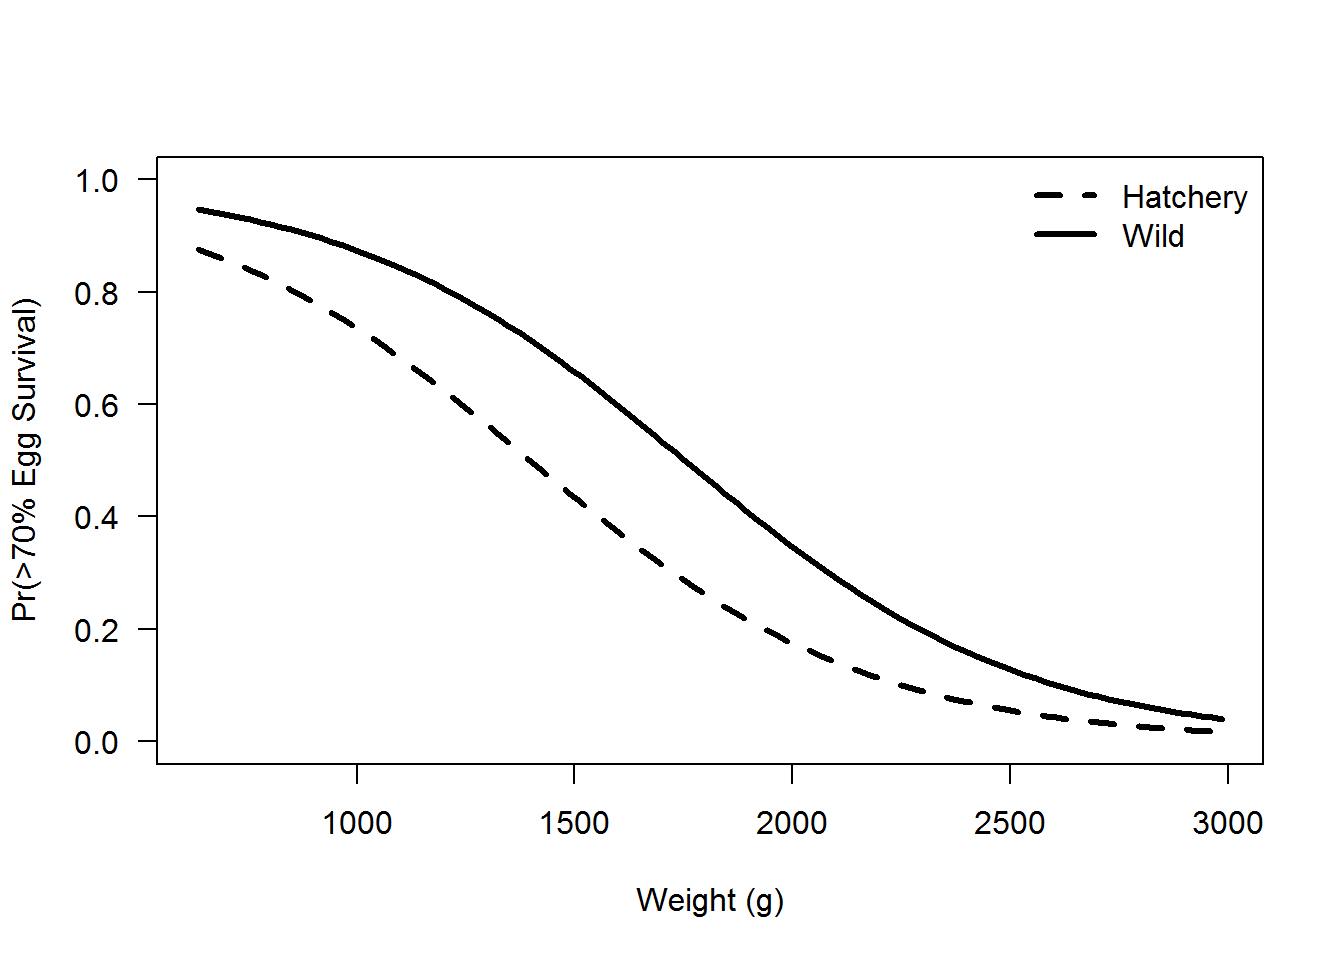
\includegraphics{au-r-workshop_files/figure-latex/unnamed-chunk-131-1} \end{center}

Look for an interaction (all the code is the same except use
\texttt{glm(binary\ \textasciitilde{}\ type\ *\ weight)} instead of
\texttt{glm(binary\ \textasciitilde{}\ type\ +\ weight)} and change
everything to \texttt{fit4} instead of \texttt{fit3}).

\begin{center}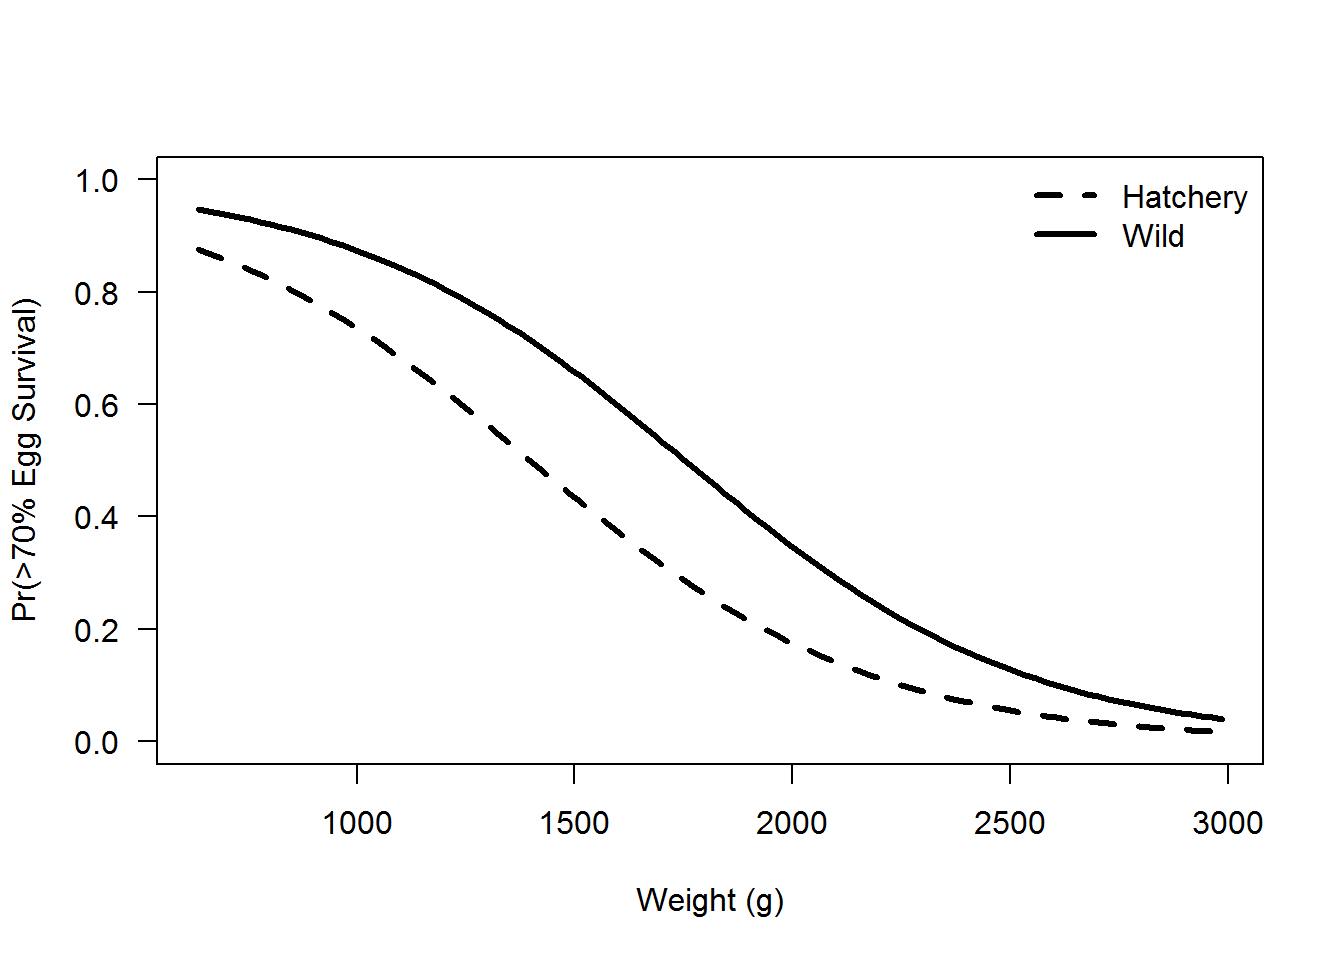
\includegraphics{au-r-workshop_files/figure-latex/unnamed-chunk-132-1} \end{center}

\subsection{AIC Model Selection}\label{aic-model-selection-1}

You may have noticed that you just did the same analysis with
\texttt{binary} as the response instead of \texttt{fecund}. Perform an
AIC analysis to determine which model is likely to be best for
prediction:

\begin{Shaded}
\begin{Highlighting}[]
\NormalTok{tab =}\StringTok{ }\KeywordTok{AIC}\NormalTok{(fit1, fit2, fit3, fit4)}
\NormalTok{tab[}\KeywordTok{order}\NormalTok{(tab}\OperatorTok{$}\NormalTok{AIC),]}
\end{Highlighting}
\end{Shaded}

\begin{verbatim}
##      df      AIC
## fit1  2 45.40720
## fit4  3 46.00622
## fit2  2 50.07577
## fit3  4 50.42090
\end{verbatim}

Oddly enough, the two best models are the simplest one and the most
complex one, with \texttt{fit1} being the best, but not by a large
margin.

\section{Probability Distributions}\label{dists}

A probability distribution is a way of representing the probability of
an event or value of a parameter and they are central to statistical
theory. Some of the most commonly used distributions are summarized in
Table \ref{tab:dist-table-pdf}, along with the suffixes of the functions
in R that correspond to each distribution\footnote{For an excellent and
  ecologically-focused description of probability distributions,
  checkout Ben Bolker's book, \emph{Ecological Models and Data in R}.
  There is a free proof version online:
  \url{https://ms.mcmaster.ca/~bolker/emdbook/book.pdf}}.

\begin{table}

\caption{\label{tab:dist-table-pdf}A brief description of probability distributions commonly used in ecological problems, including the function suffix in R.}
\centering
\begin{tabular}[t]{l>{\raggedright\arraybackslash}p{20em}>{\ttfamily}l}
\toprule
\textbf{Distribution} & \textbf{Description} & \textbf{R Suffix}\\
\midrule
\addlinespace[0.3em]
\multicolumn{3}{l}{\textbf{Continuous}}\\
\hline
\hspace{1em}Normal & Models the relative frequency of outcomes that are symmetric around a mean, can be negative & -norm()\\
\hspace{1em}Lognormal & Models the relative frequency of outcomes that are normally-distributed on the log-scale & -lnorm()\\
\hspace{1em}Uniform & Models values that are between two endpoints and that all occur with the same frequency & -unif()\\
\hspace{1em}Beta & Models values that are between 0 and 1 & -beta()\\
\addlinespace[0.3em]
\multicolumn{3}{l}{\textbf{Discrete}}\\
\hline
\hspace{1em}Binomial & Models the number of successes from a given number of trials when there are only two possible outcomes and all trials have the same probability of success & -binom()\\
\hspace{1em}Multinomial & The same as the binomial distribution, but when there are more than two possible outcomes & -multinom()\\
\hspace{1em}Poisson & Used for count data in cases where the variance and mean are roughly equal & -pois()\\
\bottomrule
\end{tabular}
\end{table}

In R, there are four different ways to use each of these distribution
functions (each has a separate prefix):

\begin{itemize}
\tightlist
\item
  \textbf{The probability density (or mass) function} (\texttt{d-}): the
  height of the probability distribution function at some given value of
  the random variable.
\item
  \textbf{The cumulative density function} (\texttt{p-}): what is the
  sum of the probability densities for all random variables below the
  input argument \texttt{q}.
\item
  \textbf{The quantile function} (\texttt{-q}): what value of the random
  variable do \texttt{p}\% fall below?
\item
  \textbf{The random deviates function} (\texttt{-r}): generates random
  variables from the distribution in proportion to their probability
  density.
\end{itemize}

Suppose that \(x\) represents the length of individual age 6 largemouth
bass in your private fishing pond. Assume that
\(x \sim N(\mu=500, \sigma=50)\)\footnote{English: \(x\) is a normal
  random variable with mean equal to 500 and standard deviation equal to
  50}. Here is the usage of each of the distribution functions and a
plot illustrating them:

\begin{Shaded}
\begin{Highlighting}[]
\CommentTok{# parameters}
\NormalTok{mu =}\StringTok{ }\DecValTok{500}\NormalTok{; sig =}\StringTok{ }\DecValTok{50}

\CommentTok{# a sequence of possible random variables (fish lengths)}
\NormalTok{lengths =}\StringTok{ }\KeywordTok{seq}\NormalTok{(}\DecValTok{200}\NormalTok{, }\DecValTok{700}\NormalTok{, }\DataTypeTok{length =} \DecValTok{100}\NormalTok{)}

\CommentTok{# a sequence of possible cumulative probabilities}
\NormalTok{cprobs =}\StringTok{ }\KeywordTok{seq}\NormalTok{(}\DecValTok{0}\NormalTok{, }\DecValTok{1}\NormalTok{, }\DataTypeTok{length =} \DecValTok{100}\NormalTok{)}

\NormalTok{densty =}\StringTok{ }\KeywordTok{dnorm}\NormalTok{(}\DataTypeTok{x =}\NormalTok{ lengths, }\DataTypeTok{mean =}\NormalTok{ mu, }\DataTypeTok{sd =}\NormalTok{ sig)  }\CommentTok{# takes specific lengths}
\NormalTok{cuprob =}\StringTok{ }\KeywordTok{pnorm}\NormalTok{(}\DataTypeTok{q =}\NormalTok{ lengths, }\DataTypeTok{mean =}\NormalTok{ mu, }\DataTypeTok{sd =}\NormalTok{ sig)  }\CommentTok{# takes specific lengths}
\NormalTok{quants =}\StringTok{ }\KeywordTok{qnorm}\NormalTok{(}\DataTypeTok{p =}\NormalTok{ cprobs, }\DataTypeTok{mean =}\NormalTok{ mu, }\DataTypeTok{sd =}\NormalTok{ sig)   }\CommentTok{# takes specific probabilities}
\NormalTok{random =}\StringTok{ }\KeywordTok{rnorm}\NormalTok{(}\DataTypeTok{n =} \FloatTok{1e4}\NormalTok{, }\DataTypeTok{mean =}\NormalTok{ mu, }\DataTypeTok{sd =}\NormalTok{ sig)      }\CommentTok{# takes a number of random deviates to make}

\CommentTok{# set up plotting region: see ?par for more details}
\CommentTok{# notice the tricks to clean up the plot}
\KeywordTok{par}\NormalTok{(}
  \DataTypeTok{mfrow =} \KeywordTok{c}\NormalTok{(}\DecValTok{2}\NormalTok{,}\DecValTok{2}\NormalTok{),    }\CommentTok{# set up 2x2 regions}
  \DataTypeTok{mar =} \KeywordTok{c}\NormalTok{(}\DecValTok{3}\NormalTok{,}\DecValTok{3}\NormalTok{,}\DecValTok{3}\NormalTok{,}\DecValTok{1}\NormalTok{),  }\CommentTok{# set narrower margins}
  \DataTypeTok{xaxs =} \StringTok{"i"}\NormalTok{,        }\CommentTok{# remove "x-buffer"}
  \DataTypeTok{yaxs =} \StringTok{"i"}\NormalTok{,        }\CommentTok{# remove "y-buffer"}
  \DataTypeTok{mgp =} \KeywordTok{c}\NormalTok{(}\DecValTok{2}\NormalTok{,}\FloatTok{0.4}\NormalTok{,}\DecValTok{0}\NormalTok{),  }\CommentTok{# bring in axis titles ([1]) and tick labels ([2])}
  \DataTypeTok{tcl =} \OperatorTok{-}\FloatTok{0.25}        \CommentTok{# shorten tick marks}
\NormalTok{)}

\KeywordTok{plot}\NormalTok{(densty }\OperatorTok{~}\StringTok{ }\NormalTok{lengths, }\DataTypeTok{type =} \StringTok{"l"}\NormalTok{, }\DataTypeTok{lwd =} \DecValTok{3}\NormalTok{, }\DataTypeTok{main =} \StringTok{"dnorm()"}\NormalTok{,}
     \DataTypeTok{xlab =} \StringTok{"Fish Length (mm)"}\NormalTok{, }\DataTypeTok{ylab =} \StringTok{"Density"}\NormalTok{, }\DataTypeTok{las =} \DecValTok{1}\NormalTok{,}
     \DataTypeTok{yaxt =} \StringTok{"n"}\NormalTok{) }\CommentTok{# turns off y-axis}
\KeywordTok{axis}\NormalTok{(}\DataTypeTok{side =} \DecValTok{2}\NormalTok{, }\DataTypeTok{at =} \KeywordTok{c}\NormalTok{(}\FloatTok{0.002}\NormalTok{, }\FloatTok{0.006}\NormalTok{), }\DataTypeTok{labels =} \KeywordTok{c}\NormalTok{(}\FloatTok{0.002}\NormalTok{, }\FloatTok{0.006}\NormalTok{), }\DataTypeTok{las =} \DecValTok{2}\NormalTok{)}
\KeywordTok{plot}\NormalTok{(cuprob }\OperatorTok{~}\StringTok{ }\NormalTok{lengths, }\DataTypeTok{type =} \StringTok{"l"}\NormalTok{, }\DataTypeTok{lwd =} \DecValTok{3}\NormalTok{, }\DataTypeTok{main =} \StringTok{"pnorm()"}\NormalTok{,}
     \DataTypeTok{xlab =} \StringTok{"Fish Length (mm)"}\NormalTok{, }\DataTypeTok{ylab =} \StringTok{"Cumulative Probability"}\NormalTok{, }\DataTypeTok{las =} \DecValTok{1}\NormalTok{)}
\KeywordTok{plot}\NormalTok{(quants }\OperatorTok{~}\StringTok{ }\NormalTok{cprobs, }\DataTypeTok{type =} \StringTok{"l"}\NormalTok{, }\DataTypeTok{lwd =} \DecValTok{3}\NormalTok{, }\DataTypeTok{main =} \StringTok{"qnorm()"}\NormalTok{,}
     \DataTypeTok{xlab =} \StringTok{"P"}\NormalTok{, }\DataTypeTok{ylab =} \StringTok{"P Quantile Length (mm)"}\NormalTok{, }\DataTypeTok{las =} \DecValTok{1}\NormalTok{)}
\KeywordTok{hist}\NormalTok{(random, }\DataTypeTok{breaks =} \DecValTok{50}\NormalTok{, }\DataTypeTok{col =} \StringTok{"grey"}\NormalTok{, }\DataTypeTok{main =} \StringTok{"rnorm()"}\NormalTok{,}
     \DataTypeTok{xlab =} \StringTok{"Fish Length (mm)"}\NormalTok{, }\DataTypeTok{ylab =} \StringTok{"Frequency"}\NormalTok{, }\DataTypeTok{las =} \DecValTok{1}\NormalTok{)}
\KeywordTok{box}\NormalTok{() }\CommentTok{# add borders to the histogram}
\end{Highlighting}
\end{Shaded}

\begin{figure}

{\centering 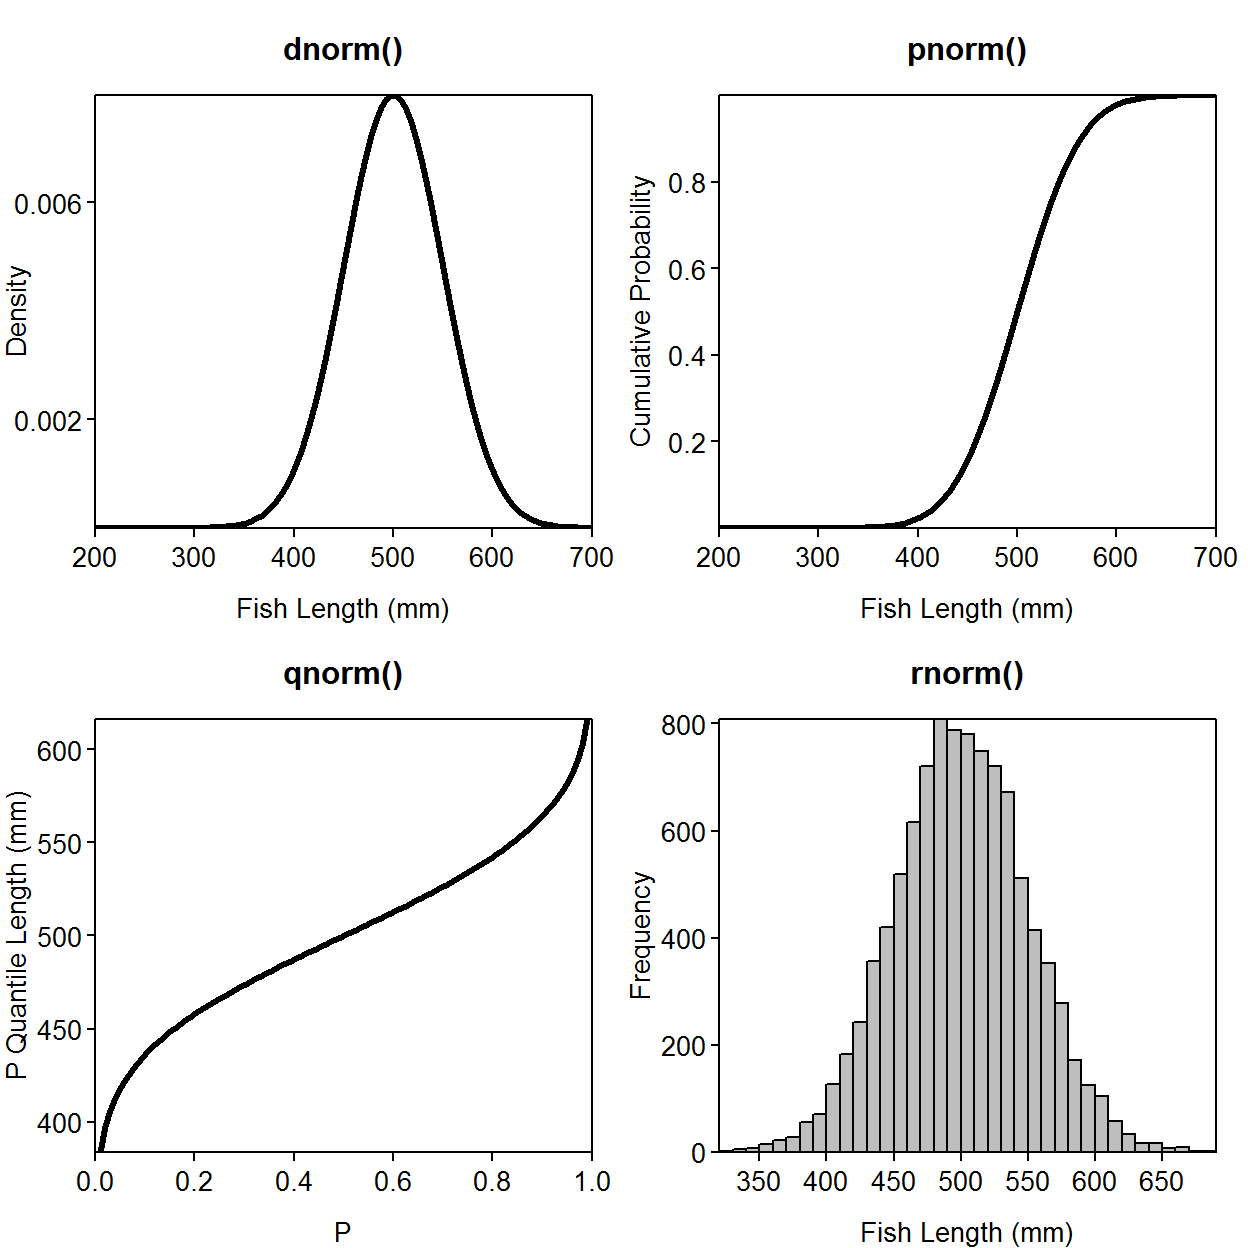
\includegraphics{au-r-workshop_files/figure-latex/norm-plots-1} 

}

\caption{The four `-norm` functions with input (x-axis) and output (y-axis) displayed.}\label{fig:norm-plots}
\end{figure}

Notice that \texttt{pnorm()} and \texttt{qnorm()} are inverses of one
another: if you put the output of one into the output of the other, you
get the original input back:

\begin{Shaded}
\begin{Highlighting}[]
\KeywordTok{qnorm}\NormalTok{(}\KeywordTok{pnorm}\NormalTok{(}\DecValTok{0}\NormalTok{))}
\end{Highlighting}
\end{Shaded}

\begin{verbatim}
## [1] 0
\end{verbatim}

\texttt{pnorm(0)} asks R to find the probability that \(x\) is less than
zero for the standard normal distribution (\(N(0,1)\) - this is the
default if you don't specify \texttt{mean} and \texttt{sig}).
\texttt{qnorm(pnorm(0))} asks R to find the value of \(x\) that
\texttt{pnorm(0)} * 100\% of the possible values fall below. If the
nesting is confusing, this line is the same as:

\begin{Shaded}
\begin{Highlighting}[]
\NormalTok{p =}\StringTok{ }\KeywordTok{pnorm}\NormalTok{(}\DecValTok{0}\NormalTok{)}
\KeywordTok{qnorm}\NormalTok{(p)}
\end{Highlighting}
\end{Shaded}

\section{Bonus Topic: Non-linear Regression}\label{nls}

You fitted linear and logistic regression models in Sections
\ref{regression} and \ref{logis-regression}, however, R allows you to
fit non-linear regression models as well.

First, read the data into R:

\begin{Shaded}
\begin{Highlighting}[]
\NormalTok{dat =}\StringTok{ }\KeywordTok{read.csv}\NormalTok{(}\StringTok{"../Data/feeding.csv"}\NormalTok{); }\KeywordTok{summary}\NormalTok{(dat)}
\end{Highlighting}
\end{Shaded}

\begin{verbatim}
##       prey            cons      
##  Min.   : 1.00   Min.   : 1.00  
##  1st Qu.:11.25   1st Qu.: 8.00  
##  Median :26.00   Median :11.00  
##  Mean   :25.08   Mean   : 9.92  
##  3rd Qu.:37.75   3rd Qu.:13.00  
##  Max.   :49.00   Max.   :15.00
\end{verbatim}

These are hypothetical data from an experiment in which you were
interested in quantifying the functional feeding response\footnote{A
  functional response is the number of prey consumed by a predator at
  various prey densities} of a fish predator on zooplankton in an
aquarium. You experimentally manipulated the prey density
(\texttt{prey}) and counted how many prey items were consumed
(\texttt{cons}).

Plot the data:

\begin{Shaded}
\begin{Highlighting}[]
\KeywordTok{plot}\NormalTok{(cons }\OperatorTok{~}\StringTok{ }\NormalTok{prey, }\DataTypeTok{data =}\NormalTok{ dat, }\DataTypeTok{cex =} \FloatTok{1.5}\NormalTok{, }\DataTypeTok{pch =} \DecValTok{16}\NormalTok{, }\DataTypeTok{col =} \StringTok{"grey"}\NormalTok{)}
\end{Highlighting}
\end{Shaded}

\begin{center}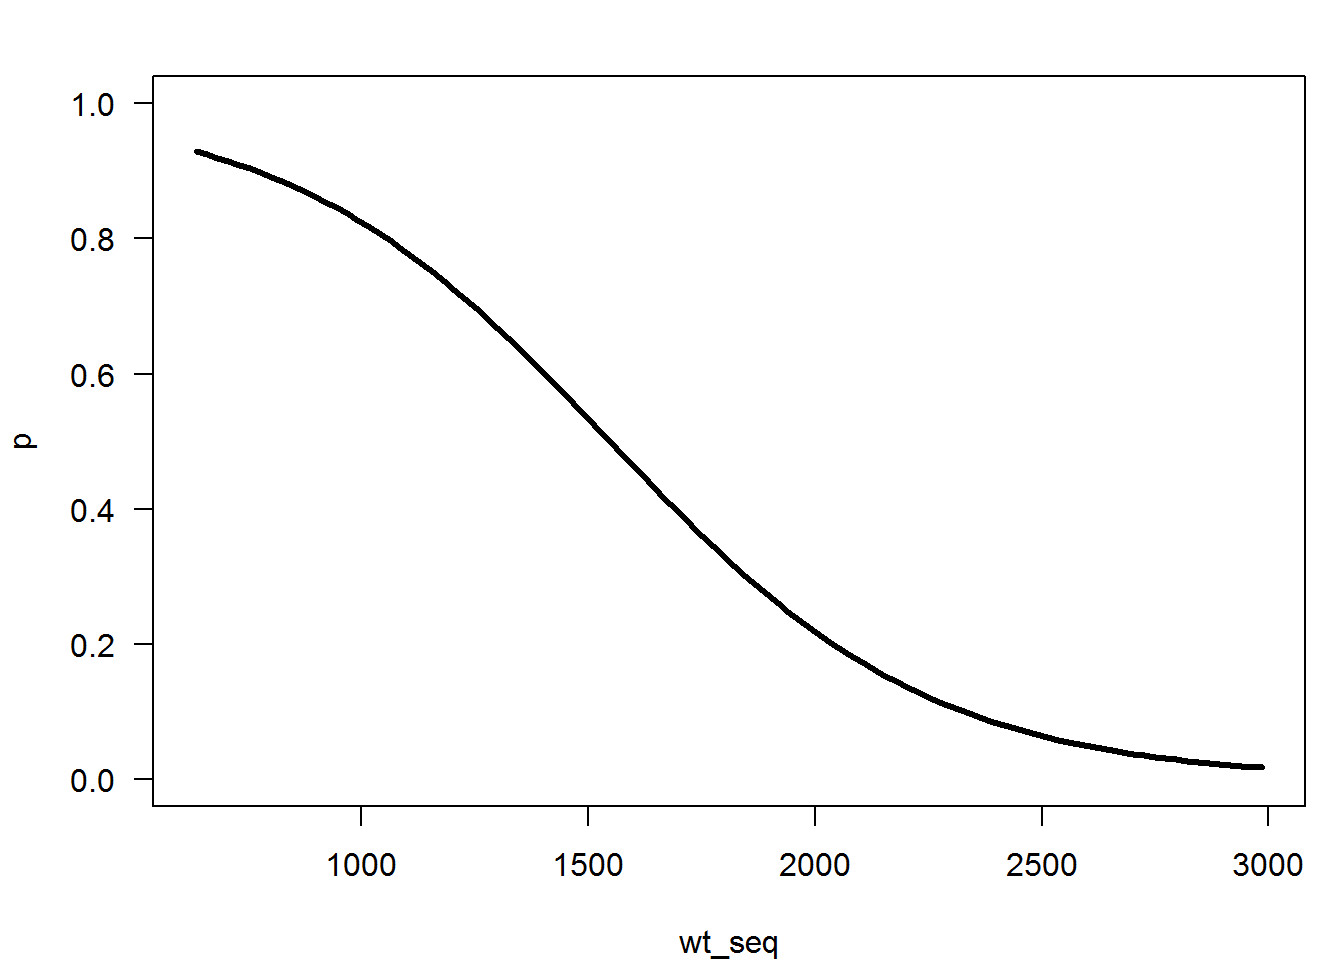
\includegraphics{au-r-workshop_files/figure-latex/unnamed-chunk-138-1} \end{center}

You can see a distinct non-linearity to the relationship. The Holling
Type II functional response\footnote{This function rises quickly at low
  prey densities, but saturates at high densities} has this functional
form:

\begin{equation}
  y_i=\frac{ax_i}{1+ahx_i} + \varepsilon_i, \varepsilon_i \sim N(0, \sigma)
\label{eq:func-resp}
\end{equation}

where \(x_i\) is \texttt{prey} and \(y_i\) is \texttt{cons}.

You can fit this model in R using the \texttt{nls()} function:

\begin{Shaded}
\begin{Highlighting}[]
\NormalTok{fit =}\StringTok{ }\KeywordTok{nls}\NormalTok{(cons }\OperatorTok{~}\StringTok{ }\NormalTok{(a }\OperatorTok{*}\StringTok{ }\NormalTok{prey)}\OperatorTok{/}\NormalTok{(}\DecValTok{1} \OperatorTok{+}\StringTok{ }\NormalTok{a }\OperatorTok{*}\StringTok{ }\NormalTok{h }\OperatorTok{*}\StringTok{ }\NormalTok{prey), }\DataTypeTok{data =}\NormalTok{ dat,}
          \DataTypeTok{start =} \KeywordTok{c}\NormalTok{(}\DataTypeTok{a =} \DecValTok{3}\NormalTok{, }\DataTypeTok{h =} \FloatTok{0.1}\NormalTok{))}
\end{Highlighting}
\end{Shaded}

In general, it behaves very similarly to the \texttt{lm()} function,
however there are a few differences:

\begin{itemize}
\tightlist
\item
  You need to specify the functional form of the curve you are
  attempting to fit. In using \texttt{lm()}, the terms are all additive
  (e.g., \texttt{type\ +\ weight}), but in using \texttt{nls()}, this is
  not the case. For example, note the use of division.
\item
  You may need to provide starting values for the parameters
  (coefficients) you are estimating. This is because \texttt{nls()} will
  use a search algorithm to find the parameters of the best fit line,
  and it may need to have a reasonable idea of where to start looking
  for it to work properly.
\item
  You cannot plot the fit using \texttt{abline()} anymore, because you
  have more parameters than just a slope and intercept, and the
  relationship between \(x\) and \(y\) is no longer linear.
\end{itemize}

Despite these differences, you can obtain similar output as from
\texttt{lm()} by using the \texttt{summary()}, \texttt{coef()}, and
\texttt{predict()} functions. Draw the fitted line over top of the data:

\begin{Shaded}
\begin{Highlighting}[]
\NormalTok{prey_seq =}\StringTok{ }\KeywordTok{seq}\NormalTok{(}\KeywordTok{min}\NormalTok{(dat}\OperatorTok{$}\NormalTok{prey), }\KeywordTok{max}\NormalTok{(dat}\OperatorTok{$}\NormalTok{prey), }\DataTypeTok{length =} \DecValTok{100}\NormalTok{)}
\NormalTok{cons_seq =}\StringTok{ }\KeywordTok{predict}\NormalTok{(fit, }\DataTypeTok{newdata =} \KeywordTok{data.frame}\NormalTok{(}\DataTypeTok{prey =}\NormalTok{ prey_seq))}

\KeywordTok{plot}\NormalTok{(cons }\OperatorTok{~}\StringTok{ }\NormalTok{prey, }\DataTypeTok{data =}\NormalTok{ dat, }\DataTypeTok{cex =} \FloatTok{1.5}\NormalTok{, }\DataTypeTok{pch =} \DecValTok{16}\NormalTok{, }\DataTypeTok{col =} \StringTok{"grey"}\NormalTok{)}
\KeywordTok{lines}\NormalTok{(cons_seq }\OperatorTok{~}\StringTok{ }\NormalTok{prey_seq, }\DataTypeTok{lwd =} \DecValTok{3}\NormalTok{)}
\end{Highlighting}
\end{Shaded}

\begin{center}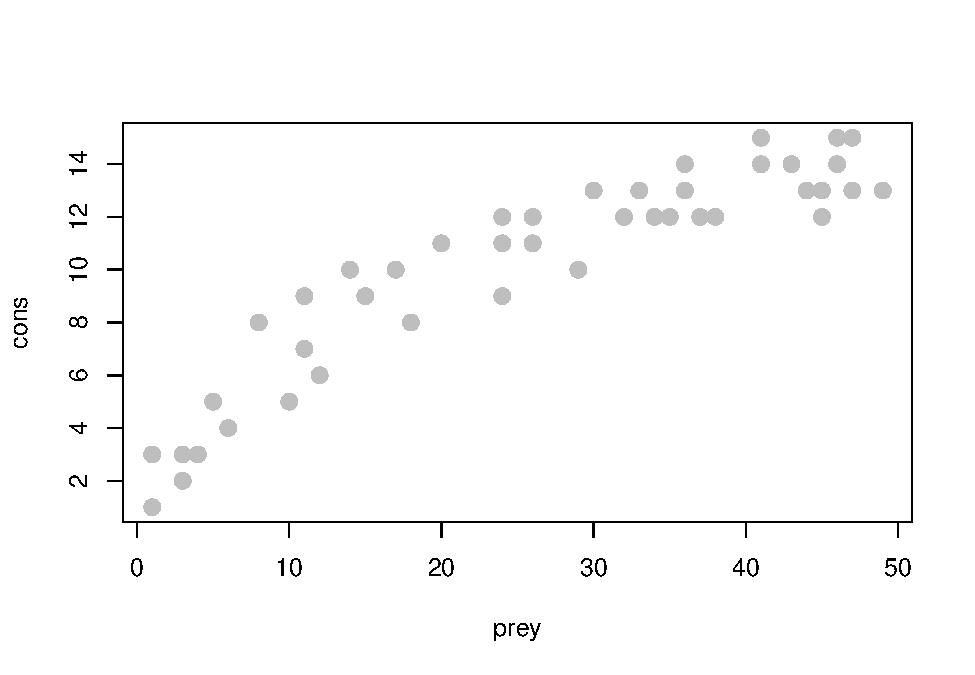
\includegraphics{au-r-workshop_files/figure-latex/unnamed-chunk-140-1} \end{center}

\begin{center}\rule{0.5\linewidth}{\linethickness}\end{center}

\section*{Exercise 3}\label{exercise-3}
\addcontentsline{toc}{section}{Exercise 3}

You should create a new R script called \texttt{Ex3.R} in your working
directory for this chapter. You will again be using the
\texttt{sockeye.csv} data found in \citet{sockeye-cite}.

\emph{The solutions to this exercise are found at the end of this book
(\protect\hyperlink{ex3-answers}{here}). You are \textbf{strongly
recommended} to make a good attempt at completing this exercise on your
own and only look at the solutions when you are truly stumped.}

\begin{enumerate}
\def\labelenumi{\arabic{enumi}.}
\item
  Perform the same analyses as conducted in Section \ref{lm} (simple
  linear regression, ANOVA, ANCOVA, ANCOVA with interaction), using
  \texttt{egg\_size} as the response variable. The predictor variables
  you should use are \texttt{type} (categorical) and \texttt{year}. You
  should plot the fit for each model separately and perform an AIC
  analysis. Practice interpretting the coefficient estimates.
\item
  Perform the same analyses as conducted in Section \ref{glms}, this
  time using a success being having greater than 80\% survival to the
  eyed-egg stage. Use \texttt{egg\_size} and \texttt{type} as the
  predictor variables. You should plot the fitted lines for each model
  separately and perform an AIC analysis. Practice interpretting the
  coefficient estimates.
\item
  Make the same graphic as in Figure \ref{fig:norm-plots} with at least
  one of the other distributions listed in Table
  \ref{tab:dist-table-pdf} (other than the multinomial - being a
  multivariate distribution, it wouldn't work well with this code). Try
  thinking of a variable from your work that meets the uses of each
  distribution in Table \ref{tab:dist-table-pdf} (or one that's not
  listed). If you run into trouble, check out the help file for that
  distribution\footnote{Executing \texttt{?rnorm} or any other of the
    \texttt{-norm()} functions will take you to a page with info on all
    four function types for that distribution}. \#\#\# Exercise 3 Bonus
  \{-\}
\item
  Fit a von Bertalannfy growth model to the data found in the
  \texttt{growth.csv} data file. Visit Section \ref{boot-test-ex}
  (particularly Equation \eqref{eq:vonB}) for details on this model. Use
  the initial values: \texttt{linf\ =\ 600}, \texttt{k\ =\ 0.3},
  \texttt{t0\ =\ -0.2}. Plot the fitted line over top of the data.
\end{enumerate}

\chapter{Monte Carlo Methods}\label{ch4}

\section*{Chapter Overview}\label{chapter-overview-3}
\addcontentsline{toc}{section}{Chapter Overview}

Simulation modeling is one of the primary reasons to move away from
spreadsheet-type programs (like Microsoft Excel) and into a program like
R. R allows you to replicate the same (possibly complex and detailed)
calculations over and over with different random values. You can then
summarize and plot the results of these replicated calculations all
within the same program. Analyses of this type are \textbf{Monte Carlo
methods}: they randomly sample from a set of quanities for the purpose
of generating and summarizing a distribution of some statistic related
to the sampled quantities. If this concept is confusing, hopefully this
chapter will clarify.

In this chapter, you will learn the basic skills needed for simulation
(i.e., Monte Carlo) modeling in R including:

\begin{itemize}
\tightlist
\item
  introduce randomness to a model
\item
  repeat calculations many times
\item
  summarization of many values from a distribution
\item
  more advanced function writing
\end{itemize}

\textbf{IMPORTANT NOTE}: If you did not attend the sessions
corresponding to Chapters \ref{ch1} or \ref{ch2} or \ref{ch3}, you are
recommended to walk through the material found in those chapters before
proceeding to this material. Remember that if you are confused about a
topic, you can use \textbf{CTRL + F} to find previous cases where that
topic has been discussed in this book.

\section*{Before You Begin}\label{before-you-begin-2}
\addcontentsline{toc}{section}{Before You Begin}

You should create a new directory and R script for your work in this
Chapter. Create a new R script called \texttt{Ch4.R} and save it in the
directory \texttt{C:/Users/YOU/Documents/R-Book/Chapter4}. Set your
working directory to that location. Revisit the material in Sections
\ref{scripts} and \ref{working-dir} for more details on these steps.

\section*{Layout of This Chapter}\label{layout-of-this-chapter}
\addcontentsline{toc}{section}{Layout of This Chapter}

This chapter is divided into two main sections:

\begin{itemize}
\item
  \textbf{Required Material} (Sections \ref{randomness} -
  \ref{mc-summaries}) which is necessary to understand the examples in
  this chapter and the subsequent chapters
\item
  \textbf{Example Cases} (Sections \ref{sim-examples} and
  \ref{resample-examples}) which apply the skills learned in the
  required material. In the workshop session, you will walkthrough 2-3
  of these example cases at the choice of the group of the participants.
  If you are interested in simulation modeling, you are suggested to
  work through all of the example cases, as slightly different tricks
  will be shown in the different examples.
\end{itemize}

\section{Introducing Randomness}\label{randomness}

A critical part of simulation modeling is the use of random processes. A
\textbf{random process} is one that generates a different outcome
according to some rules each time it is executed. They are tightly
linked to the concept of \textbf{uncertainty}: you are unsure about the
outcome the next time the process is executed. There are two basic ways
to introduce randomness in R: \textbf{random deviates} and
\textbf{resampling}.

\subsection{Random deviates}\label{random-deviates}

In Section \ref{dists}, you learned about using probability
distributions in R. One of the uses was the \texttt{r-} family of
distribution functions. These functions create random numbers following
a random process specified by a probability distribution.

Consider animal survival as an example. At the end of each year, each
individual alive at the start can either live or die. There are two
outcomes here, and suppose each animal has an 80\% chance of surviving.
The number of individuals that survive is the result of a
\textbf{binomial random process} in which there were \(n\) individuals
alive at the start of this year and \(p\) is the probability that any
one individual survives to the next year. You can execute one binomial
random process where \(p = 0.8\) and \(n = 100\) like this:

\begin{Shaded}
\begin{Highlighting}[]
\KeywordTok{rbinom}\NormalTok{(}\DataTypeTok{n =} \DecValTok{1}\NormalTok{, }\DataTypeTok{size =} \DecValTok{100}\NormalTok{, }\DataTypeTok{prob =} \FloatTok{0.8}\NormalTok{)}
\end{Highlighting}
\end{Shaded}

\begin{verbatim}
## [1] 80
\end{verbatim}

The result you get will almost certainly be different from the one
printed here. That is the random component.

You can execute many such binomial processes by changing the \texttt{n}
argument. Plot the distribution of expected surviving individuals:

\begin{Shaded}
\begin{Highlighting}[]
\NormalTok{survivors =}\StringTok{ }\KeywordTok{rbinom}\NormalTok{(}\DecValTok{1000}\NormalTok{, }\DecValTok{100}\NormalTok{, }\FloatTok{0.8}\NormalTok{)}
\KeywordTok{hist}\NormalTok{(survivors, }\DataTypeTok{col =} \StringTok{"skyblue"}\NormalTok{)}
\end{Highlighting}
\end{Shaded}

\begin{center}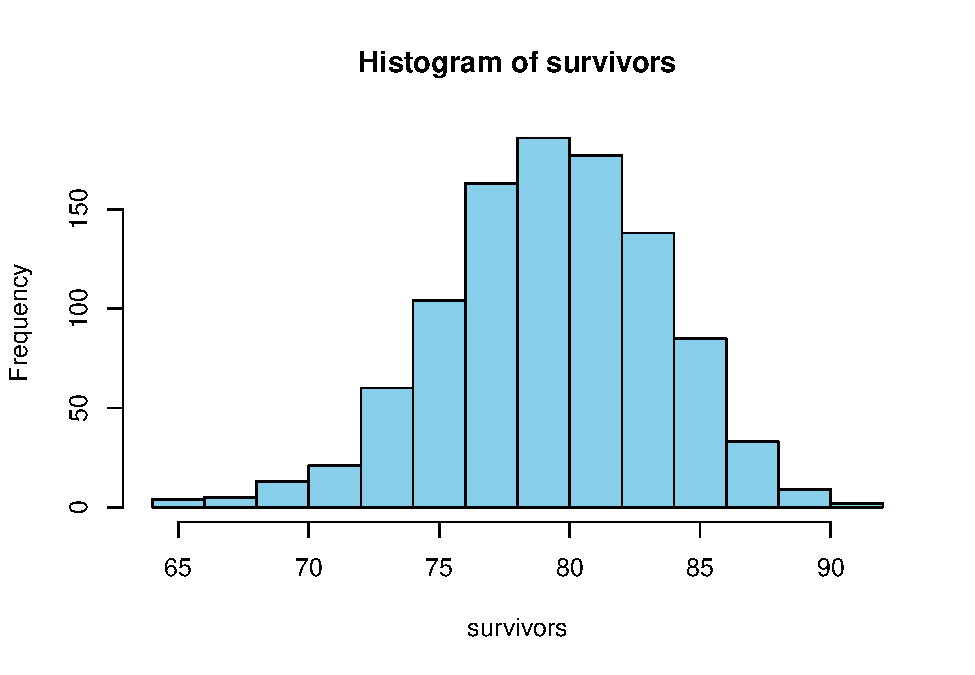
\includegraphics{au-r-workshop_files/figure-latex/unnamed-chunk-144-1} \end{center}

Another random process is the \textbf{lognormal process}: it generates
random numbers such that the log of the values are normally-distributed
with mean equal to \texttt{logmean} and standard deviation equal to
\texttt{logsd}:

\begin{Shaded}
\begin{Highlighting}[]
\KeywordTok{hist}\NormalTok{(}\KeywordTok{rlnorm}\NormalTok{(}\DecValTok{1000}\NormalTok{, }\DecValTok{0}\NormalTok{, }\FloatTok{0.1}\NormalTok{), }\DataTypeTok{col =} \StringTok{"skyblue"}\NormalTok{)}
\end{Highlighting}
\end{Shaded}

\begin{center}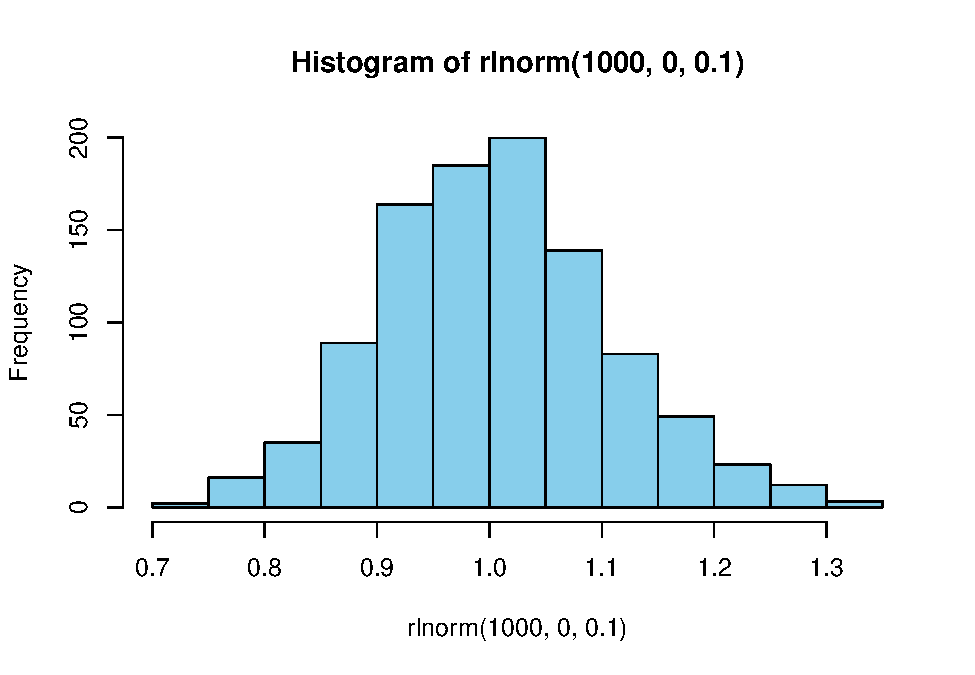
\includegraphics{au-r-workshop_files/figure-latex/unnamed-chunk-145-1} \end{center}

There are many random processes you can use in R. Checkout Table
\ref{tab:dist-table-pdf} for more examples as well as the help files for
each individual function for more details.

\subsection{Resampling}\label{resampling}

Using random deviates works great for creating new random numbers, but
what if you already have a set of numbers that you wish to introduce
randomness to? For this, you can use \textbf{resampling techniques}. In
R, the \texttt{sample()} function is used to sample \texttt{size}
elements from the vector \texttt{x}:

\begin{Shaded}
\begin{Highlighting}[]
\KeywordTok{sample}\NormalTok{(}\DataTypeTok{x =} \DecValTok{1}\OperatorTok{:}\DecValTok{10}\NormalTok{, }\DataTypeTok{size =} \DecValTok{5}\NormalTok{)}
\end{Highlighting}
\end{Shaded}

\begin{verbatim}
## [1] 2 7 3 1 9
\end{verbatim}

You can sample with replacement (where it is possible to sample the same
element two or more times):

\begin{Shaded}
\begin{Highlighting}[]
\KeywordTok{sample}\NormalTok{(}\DataTypeTok{x =} \KeywordTok{c}\NormalTok{(}\StringTok{"a"}\NormalTok{, }\StringTok{"b"}\NormalTok{, }\StringTok{"c"}\NormalTok{), }\DataTypeTok{size =} \DecValTok{10}\NormalTok{, }\DataTypeTok{replace =}\NormalTok{ T)}
\end{Highlighting}
\end{Shaded}

\begin{verbatim}
##  [1] "b" "c" "c" "c" "a" "a" "b" "b" "c" "b"
\end{verbatim}

You can set probabilities on the sampling of different
elements\footnote{If \texttt{prob} doesn't sum to 1, then it will be
  rescaled: \texttt{prob\ =\ prob/sum(prob)}}:

\begin{Shaded}
\begin{Highlighting}[]
\KeywordTok{sample}\NormalTok{(}\DataTypeTok{x =} \KeywordTok{c}\NormalTok{(}\StringTok{"live"}\NormalTok{, }\StringTok{"die"}\NormalTok{), }\DataTypeTok{size =} \DecValTok{10}\NormalTok{, }\DataTypeTok{replace =}\NormalTok{ T,}
       \DataTypeTok{prob =} \KeywordTok{c}\NormalTok{(}\FloatTok{0.8}\NormalTok{, }\FloatTok{0.2}\NormalTok{))}
\end{Highlighting}
\end{Shaded}

\begin{verbatim}
##  [1] "die"  "live" "live" "live" "live" "die"  "live" "live" "live" "live"
\end{verbatim}

Notice that this is the same as the binomial random process above, but
with only 10 trials and the printing of the outcomes rather than the
number of successes.

\section{Reproducing Randomness}\label{reproducing-randomness}

For reproducibility purposes, you may wish to get the same exact random
numbers each time you run your script. To do this, you need to set the
\textbf{random seed}, which is the starting point of the random number
generator your computer uses. If you run these two lines of code, you
should get the same result as printed here:

\begin{Shaded}
\begin{Highlighting}[]
\KeywordTok{set.seed}\NormalTok{(}\DecValTok{1234}\NormalTok{)}
\KeywordTok{rnorm}\NormalTok{(}\DecValTok{1}\NormalTok{)}
\end{Highlighting}
\end{Shaded}

\begin{verbatim}
## [1] -1.207066
\end{verbatim}

\section{Replication}\label{replication}

To use Monte Carlo methods, you need to be able to replicate some random
process many times. There are two main ways this is commonly done:
either with\texttt{replicate()} or with \texttt{for()} loops.

\subsection{\texorpdfstring{\texttt{replicate()}}{replicate()}}\label{replicate}

The \texttt{replicate()} function executes some expression many times
and returns the output from each execution. Say we have a vector
\texttt{x}, which represents 30 observations of fish length (mm):

\begin{Shaded}
\begin{Highlighting}[]
\NormalTok{x =}\StringTok{ }\KeywordTok{rnorm}\NormalTok{(}\DecValTok{30}\NormalTok{, }\DecValTok{500}\NormalTok{, }\DecValTok{30}\NormalTok{)}
\end{Highlighting}
\end{Shaded}

We wish to build the sampling distribution of the mean length ``by
hand''. We can sample randomly from it, calculate the mean, then repeat
this process many times:

\begin{Shaded}
\begin{Highlighting}[]
\NormalTok{means =}\StringTok{ }\KeywordTok{replicate}\NormalTok{(}\DataTypeTok{n =} \DecValTok{1000}\NormalTok{, }\DataTypeTok{expr =}\NormalTok{ \{}
\NormalTok{  x_i =}\StringTok{ }\KeywordTok{sample}\NormalTok{(x, }\KeywordTok{length}\NormalTok{(x), }\DataTypeTok{replace =}\NormalTok{ T)}
  \KeywordTok{mean}\NormalTok{(x_i)}
\NormalTok{\})}
\end{Highlighting}
\end{Shaded}

If we take \texttt{mean(means)} and \texttt{sd(means)}, that should be
very similar to \texttt{mean(x)} and \texttt{se(x)}. Create the
\texttt{se()} function (also shown in Section \ref{error-bars}) and
prove this to yourself:

\begin{Shaded}
\begin{Highlighting}[]
\NormalTok{se =}\StringTok{ }\ControlFlowTok{function}\NormalTok{(x) }\KeywordTok{sd}\NormalTok{(x)}\OperatorTok{/}\KeywordTok{sqrt}\NormalTok{(}\KeywordTok{length}\NormalTok{(x))}
\KeywordTok{mean}\NormalTok{(means); }\KeywordTok{mean}\NormalTok{(x)}
\end{Highlighting}
\end{Shaded}

\begin{verbatim}
## [1] 493.8096
\end{verbatim}

\begin{verbatim}
## [1] 493.4166
\end{verbatim}

\begin{Shaded}
\begin{Highlighting}[]
\KeywordTok{sd}\NormalTok{(means); }\KeywordTok{se}\NormalTok{(x)}
\end{Highlighting}
\end{Shaded}

\begin{verbatim}
## [1] 4.899929
\end{verbatim}

\begin{verbatim}
## [1] 5.044153
\end{verbatim}

\subsection{\texorpdfstring{The \texttt{for()}
loop}{The for() loop}}\label{for-loops}

In programming, a \emph{loop} is a command that does something over and
over until it reaches some point that you specify. R has a few types of
loops: \texttt{repeat()}, \texttt{while()}, and \texttt{for()}, to name
a few. \texttt{for()} loops are among the most common in simulation
modeling. A \texttt{for()} loop repeats some action for however many
times you tell it \textbf{for} each value in some vector. The syntax is:

\begin{Shaded}
\begin{Highlighting}[]
\ControlFlowTok{for}\NormalTok{ (var }\ControlFlowTok{in}\NormalTok{ seq) \{}
  \KeywordTok{expression}\NormalTok{(var)}
\NormalTok{\}}
\end{Highlighting}
\end{Shaded}

The loop calculates the expression for values of \texttt{var} for each
element in the vector \texttt{seq}. For example:

\begin{Shaded}
\begin{Highlighting}[]
\ControlFlowTok{for}\NormalTok{ (i }\ControlFlowTok{in} \DecValTok{1}\OperatorTok{:}\DecValTok{5}\NormalTok{) \{}
  \KeywordTok{print}\NormalTok{(i}\OperatorTok{^}\DecValTok{2}\NormalTok{)}
\NormalTok{\}}
\end{Highlighting}
\end{Shaded}

\begin{verbatim}
## [1] 1
## [1] 4
## [1] 9
## [1] 16
## [1] 25
\end{verbatim}

The \texttt{print()} command will be executed 5 times: once for each
value of \texttt{i}. It is the same as:

\begin{Shaded}
\begin{Highlighting}[]
\NormalTok{i =}\StringTok{ }\DecValTok{1}\NormalTok{; }\KeywordTok{print}\NormalTok{(i}\OperatorTok{^}\DecValTok{2}\NormalTok{); i =}\StringTok{ }\DecValTok{2}\NormalTok{; }\KeywordTok{print}\NormalTok{(i}\OperatorTok{^}\DecValTok{2}\NormalTok{); i =}\StringTok{ }\DecValTok{3}\NormalTok{; }\KeywordTok{print}\NormalTok{(i}\OperatorTok{^}\DecValTok{2}\NormalTok{); i =}\StringTok{ }\DecValTok{4}\NormalTok{; }\KeywordTok{print}\NormalTok{(i}\OperatorTok{^}\DecValTok{2}\NormalTok{); i =}\StringTok{ }\DecValTok{5}\NormalTok{; }\KeywordTok{print}\NormalTok{(i}\OperatorTok{^}\DecValTok{2}\NormalTok{)}
\end{Highlighting}
\end{Shaded}

If you remove the \texttt{print()} function, see what happens:

\begin{Shaded}
\begin{Highlighting}[]
\ControlFlowTok{for}\NormalTok{ (i }\ControlFlowTok{in} \DecValTok{1}\OperatorTok{:}\DecValTok{5}\NormalTok{) \{}
\NormalTok{  i}\OperatorTok{^}\DecValTok{2}
\NormalTok{\}}
\end{Highlighting}
\end{Shaded}

Nothing is printed to the console. R did the calculation, but did not
show you or store the result Often, you'll need to store the results of
the calculation in a \textbf{container object}:

\begin{Shaded}
\begin{Highlighting}[]
\NormalTok{results =}\StringTok{ }\KeywordTok{numeric}\NormalTok{(}\DecValTok{5}\NormalTok{)}
\end{Highlighting}
\end{Shaded}

This makes an empty numeric vector of length 5 that are all 0's. You can
store the output of your loop calculations in \texttt{results}:

\begin{Shaded}
\begin{Highlighting}[]
\ControlFlowTok{for}\NormalTok{ (i }\ControlFlowTok{in} \DecValTok{1}\OperatorTok{:}\DecValTok{5}\NormalTok{) \{}
\NormalTok{  results[i]=i}\OperatorTok{^}\DecValTok{2}
\NormalTok{\}}
\NormalTok{results}
\end{Highlighting}
\end{Shaded}

\begin{verbatim}
## [1]  1  4  9 16 25
\end{verbatim}

When \texttt{i\^{}2} is calculated, it will be placed in the element
\texttt{results{[}i{]}}. This was a trivial example, because you should
do things like this using R's vectorized calculation framework:
\texttt{(1:5)\^{}2} (see Section \ref{vector-math}).

However, there are times where it is advantageous to use a loop.
Particularly in cases where:

\begin{enumerate}
\def\labelenumi{\arabic{enumi}.}
\tightlist
\item
  the calculations in one element are determined from the value in
  previous elements, such as in time series models
\item
  the calculations have multiple steps
\item
  you wish to store multiple results
\item
  you wish to track the progress of your calculations
\end{enumerate}

As an illustration for item (1) above, build a (very) basic population
model. At the start of the first year, the population abundance is 1000
individuals and grows by an average factor of 1.1 per year (reproduction
and death processes result in a growth rate of 10\%) before harvest. The
growth rate varies randomly, however. Each year, the 1.1 growth factor
has variability introduced by small changes in survival and reproductive
process. Model these variations as lognormal random variables. After
production, 8\% of the population is harvested. Simulate and plot the
abundance at the end of the year for 100 years:

\begin{Shaded}
\begin{Highlighting}[]
\NormalTok{nt =}\StringTok{ }\DecValTok{100}       \CommentTok{# number of years}
\NormalTok{N =}\StringTok{ }\OtherTok{NULL}       \CommentTok{# container for abundance}
\NormalTok{N[}\DecValTok{1}\NormalTok{] =}\StringTok{ }\DecValTok{1000}    \CommentTok{# first end-of-year abundance}

\ControlFlowTok{for}\NormalTok{ (t }\ControlFlowTok{in} \DecValTok{2}\OperatorTok{:}\NormalTok{nt) \{}
  \CommentTok{# N this year is N last year * growth *}
    \CommentTok{# randomness * fraction that survive harvest}
\NormalTok{  N[t] =}\StringTok{ }\NormalTok{(N[t}\OperatorTok{-}\DecValTok{1}\NormalTok{] }\OperatorTok{*}\StringTok{ }\FloatTok{1.1} \OperatorTok{*}\StringTok{ }\KeywordTok{rlnorm}\NormalTok{(}\DecValTok{1}\NormalTok{, }\DecValTok{0}\NormalTok{, }\FloatTok{0.1}\NormalTok{)) }\OperatorTok{*}\StringTok{ }\NormalTok{(}\DecValTok{1} \OperatorTok{-}\StringTok{ }\FloatTok{0.08}\NormalTok{)}
\NormalTok{\}}

\CommentTok{# plot}
\KeywordTok{plot}\NormalTok{(N, }\DataTypeTok{type =} \StringTok{"l"}\NormalTok{, }\DataTypeTok{pch =} \DecValTok{15}\NormalTok{, }\DataTypeTok{xlab =} \StringTok{"Year"}\NormalTok{, }\DataTypeTok{ylab =} \StringTok{"Abundance"}\NormalTok{)}
\end{Highlighting}
\end{Shaded}

\begin{center}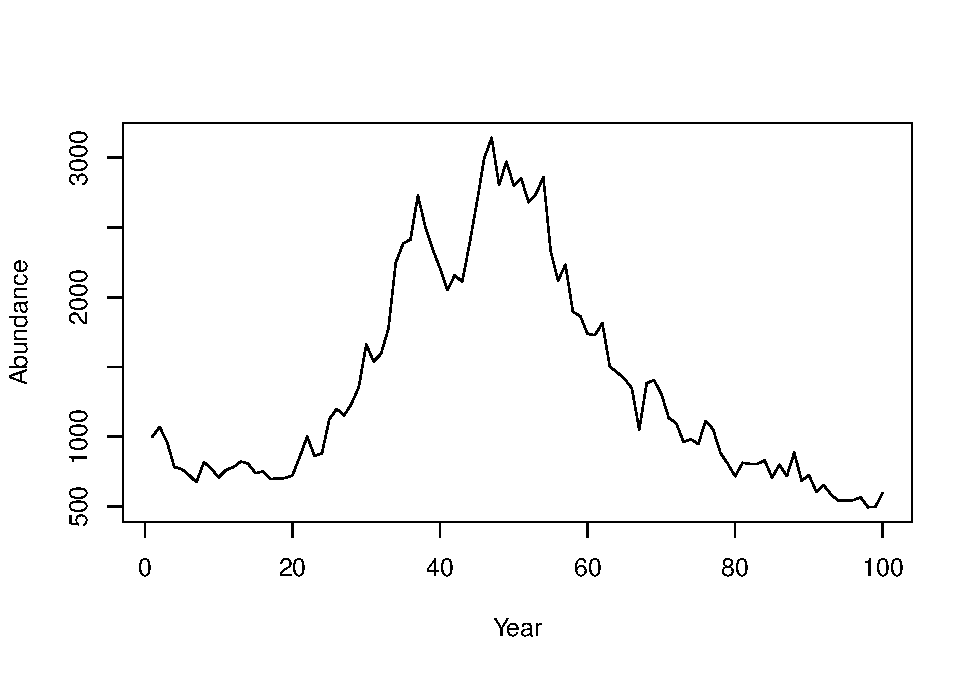
\includegraphics{au-r-workshop_files/figure-latex/unnamed-chunk-159-1} \end{center}

Examples of the other three utilities are shown in the example cases.

\section{Function Writing}\label{adv-funcs}

In Monte Carlo analyses, it is often useful to wrap code into functions.
This makes them easy to be replicated and have the settings adjusted. As
an example, turn the population model shown above into a function:

\begin{Shaded}
\begin{Highlighting}[]
\NormalTok{pop_sim =}\StringTok{ }\ControlFlowTok{function}\NormalTok{(nt, grow, sd_grow, U, }\DataTypeTok{plot =}\NormalTok{ F) \{}
\NormalTok{  N =}\StringTok{ }\OtherTok{NULL} 
\NormalTok{  N[}\DecValTok{1}\NormalTok{] =}\StringTok{ }\DecValTok{1000}
  \ControlFlowTok{for}\NormalTok{ (t }\ControlFlowTok{in} \DecValTok{2}\OperatorTok{:}\NormalTok{nt) \{}
\NormalTok{    N[t] =}\StringTok{ }\NormalTok{(N[t}\OperatorTok{-}\DecValTok{1}\NormalTok{] }\OperatorTok{*}\StringTok{ }\NormalTok{grow }\OperatorTok{*}\StringTok{ }\KeywordTok{rlnorm}\NormalTok{(}\DecValTok{1}\NormalTok{, }\DecValTok{0}\NormalTok{, sd_grow)) }\OperatorTok{*}\StringTok{ }\NormalTok{(}\DecValTok{1} \OperatorTok{-}\StringTok{ }\NormalTok{U)}
\NormalTok{  \}}
  
  \ControlFlowTok{if}\NormalTok{ (plot) \{}
    \KeywordTok{plot}\NormalTok{(N, }\DataTypeTok{type =} \StringTok{"l"}\NormalTok{, }\DataTypeTok{pch =} \DecValTok{15}\NormalTok{, }\DataTypeTok{xlab =} \StringTok{"Year"}\NormalTok{, }\DataTypeTok{ylab =} \StringTok{"Abundance"}\NormalTok{)}
\NormalTok{  \}}
  
\NormalTok{  N}
\NormalTok{\}}
\end{Highlighting}
\end{Shaded}

This function takes five inputs:

\begin{itemize}
\tightlist
\item
  \texttt{nt}: the number of years,
\item
  \texttt{grow}: the population growth rate,
\item
  \texttt{sd\_grow}: the amount of annual variability in the growth rate
\item
  \texttt{U}: the annual exploitation rate
\item
  \texttt{plot}: whether you wish to have a plot created. It has a
  default setting of \texttt{FALSE}: if you don't specify
  \texttt{plot\ =\ T} when you call \texttt{pop\_sim()}, you won't see a
  plot made.
\end{itemize}

It returns one output: the vector of population abundance.

Use your function once using the same settings as before:

\begin{Shaded}
\begin{Highlighting}[]
\KeywordTok{pop_sim}\NormalTok{(}\DecValTok{100}\NormalTok{, }\FloatTok{1.1}\NormalTok{, }\FloatTok{0.1}\NormalTok{, }\FloatTok{0.08}\NormalTok{, T)}
\end{Highlighting}
\end{Shaded}

\begin{center}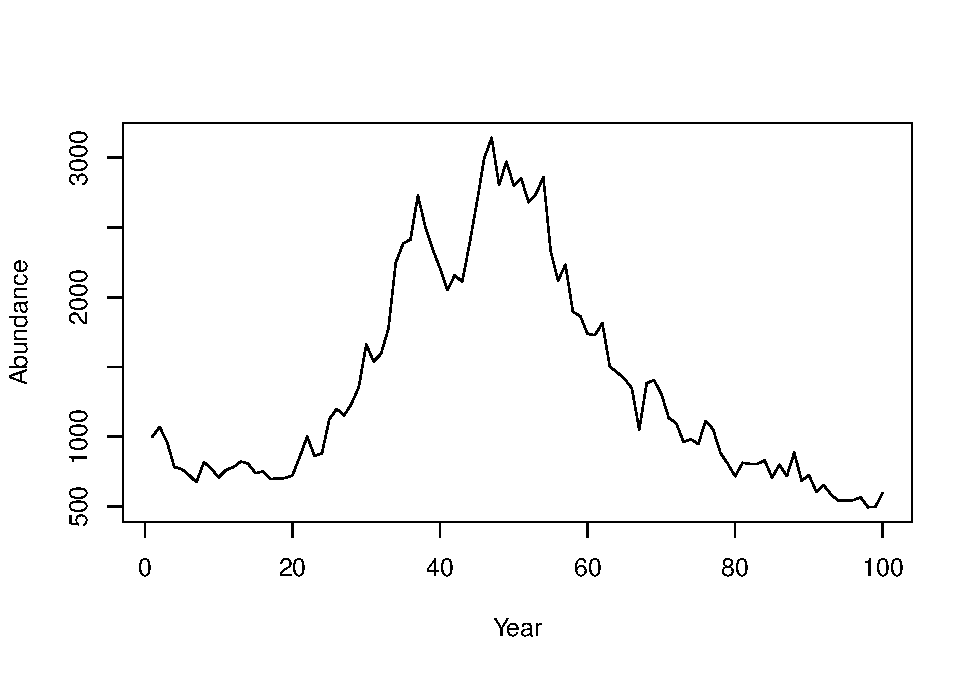
\includegraphics{au-r-workshop_files/figure-latex/unnamed-chunk-161-1} \end{center}

Now, you wish to replicate exectuing this function 1000 times. Use the
\texttt{replicate()} function to do this:

\begin{Shaded}
\begin{Highlighting}[]
\NormalTok{out =}\StringTok{ }\KeywordTok{replicate}\NormalTok{(}\DataTypeTok{n =} \DecValTok{1000}\NormalTok{, }\DataTypeTok{expr =} \KeywordTok{pop_sim}\NormalTok{(}\DecValTok{100}\NormalTok{, }\FloatTok{1.1}\NormalTok{, }\FloatTok{0.1}\NormalTok{, }\FloatTok{0.08}\NormalTok{, F))}
\end{Highlighting}
\end{Shaded}

If you do \texttt{dim(out)}, you'll see that rows are stored as years
(there are 100 of them) and columns are stored as replicates (there are
1000 of them). Notice how wrapping the code in the function made the
\texttt{replicate()} call easy.

\textbf{Here are some advantages of wrapping code like this into a
function}:

\begin{itemize}
\tightlist
\item
  If you do the same task over and over, you don't need to type all of
  the code to perform the task, just the function call.
\item
  If you need to change the way the function behaves (i.e., the function
  body), you only need to change it one place: in the function
  definition.
\item
  You can easily change the settings of the code (e.g., whether you want
  to see the plot) in one place
\item
  Function writing \textbf{can} lead to shorter scripts
\item
  Function writing \textbf{can} lead to more readable code (if people
  know what your functions do)
\end{itemize}

\section{Summarization}\label{mc-summaries}

After replicating a calculation many times, you will need to summarize
the results. Here are several examples using the \texttt{out} matrix
from Section \ref{adv-funcs}.

\subsection{Central Tendency}\label{central-tendency}

You can calculate the mean abundance each year across your iterations
using the \texttt{apply()} function (Section \ref{data-summaries}):

\begin{Shaded}
\begin{Highlighting}[]
\NormalTok{N_mean =}\StringTok{ }\KeywordTok{apply}\NormalTok{(out, }\DecValTok{1}\NormalTok{, mean)}
\NormalTok{N_mean[}\DecValTok{1}\OperatorTok{:}\DecValTok{10}\NormalTok{]}
\end{Highlighting}
\end{Shaded}

\begin{verbatim}
##  [1] 1000.000 1017.511 1033.436 1054.619 1069.542 1086.413 1107.854
##  [8] 1129.619 1145.288 1161.254
\end{verbatim}

You could do the same thing using \texttt{median} rather than
\texttt{mean}. The mode is more difficult to calculate in R, if you need
to get the mode, try to Google it\footnote{Google is an R programmer's
  best friend. There is a massive online community for R, and if you
  have a question on something, it has almost certainly been asked
  somewhere on the web.}.

\subsection{Variability}\label{variability}

One of the primary reasons to conduct a Monte Carlo analysis is to
obtain estimates of variability. You can summarize the variability
easily using the \texttt{quantile()} function:

\begin{Shaded}
\begin{Highlighting}[]
\CommentTok{# obtain the 10% and 90% quantiles each year across iterations}
\NormalTok{N_quants =}\StringTok{ }\KeywordTok{apply}\NormalTok{(out, }\DecValTok{1}\NormalTok{, }\ControlFlowTok{function}\NormalTok{(x) }\KeywordTok{quantile}\NormalTok{(x, }\KeywordTok{c}\NormalTok{(}\FloatTok{0.1}\NormalTok{, }\FloatTok{0.9}\NormalTok{)))}

\CommentTok{# plot them as a time series with the mean}
\KeywordTok{plot}\NormalTok{(N_mean, }\DataTypeTok{type =} \StringTok{"l"}\NormalTok{, }\DataTypeTok{ylim =} \KeywordTok{c}\NormalTok{(}\DecValTok{0}\NormalTok{, }\DecValTok{10000}\NormalTok{))}
\KeywordTok{lines}\NormalTok{(N_quants[}\DecValTok{1}\NormalTok{,], }\DataTypeTok{lty =} \DecValTok{2}\NormalTok{)}
\KeywordTok{lines}\NormalTok{(N_quants[}\DecValTok{2}\NormalTok{,], }\DataTypeTok{lty =} \DecValTok{2}\NormalTok{)}
\end{Highlighting}
\end{Shaded}

\begin{center}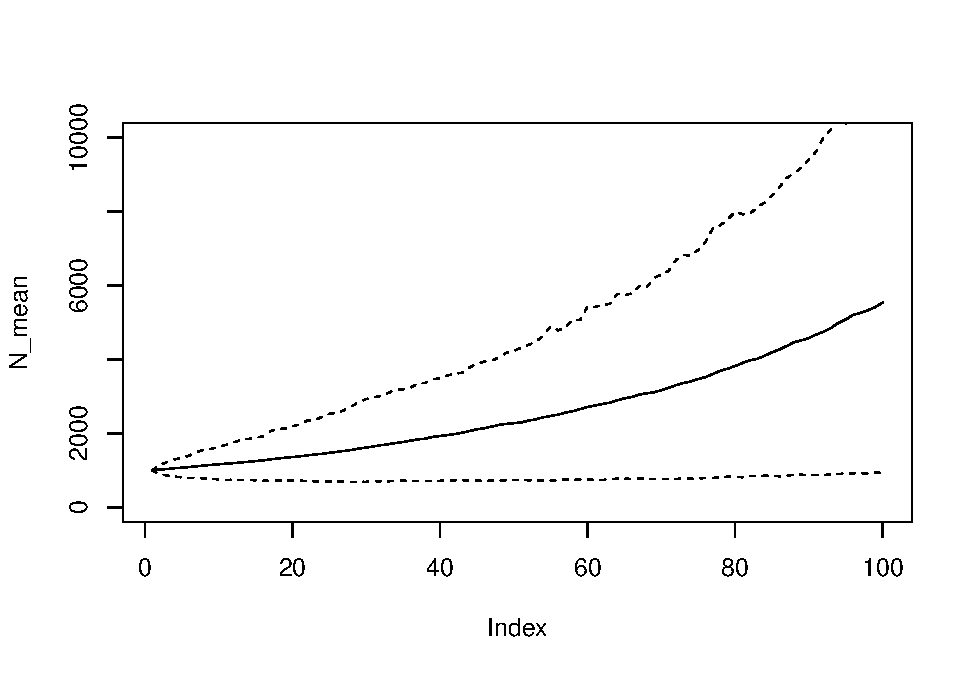
\includegraphics{au-r-workshop_files/figure-latex/unnamed-chunk-164-1} \end{center}

Notice how a user-defined function was passed to \texttt{apply()}. The
range within the two dashed lines represents the range that encompassed
the central 80\% of the random abundances each year.

\subsection{Frequencies}\label{frequencies}

Often you will want to count how many times something happened. In some
cases, the fraction of times something happened can be interpretted as a
probability.

The \texttt{table()} function is very useful for counting occurences of
discrete events. Suppose you are interested in how many of your
iterations resulted in fewer than 1000 individuals at year 10:

\begin{Shaded}
\begin{Highlighting}[]
\NormalTok{out10 =}\StringTok{ }\KeywordTok{ifelse}\NormalTok{(out[}\DecValTok{10}\NormalTok{,] }\OperatorTok{<}\StringTok{ }\DecValTok{1000}\NormalTok{, }\StringTok{"less10"}\NormalTok{, }\StringTok{"greater10"}\NormalTok{)}
\KeywordTok{table}\NormalTok{(out10)}
\end{Highlighting}
\end{Shaded}

\begin{verbatim}
## out10
## greater10    less10 
##       643       357
\end{verbatim}

Suppose you are also interested in how many of your iterations resulted
in fewer than 1100 individuals at year 20:

\begin{Shaded}
\begin{Highlighting}[]
\NormalTok{out20 =}\StringTok{ }\KeywordTok{ifelse}\NormalTok{(out[}\DecValTok{20}\NormalTok{,] }\OperatorTok{<}\StringTok{ }\DecValTok{1100}\NormalTok{, }\StringTok{"less20"}\NormalTok{, }\StringTok{"greater20"}\NormalTok{)}
\KeywordTok{table}\NormalTok{(out20)}
\end{Highlighting}
\end{Shaded}

\begin{verbatim}
## out20
## greater20    less20 
##       592       408
\end{verbatim}

Now suppose you are interested in how these two metrics are related:

\begin{Shaded}
\begin{Highlighting}[]
\KeywordTok{table}\NormalTok{(out10, out20)}
\end{Highlighting}
\end{Shaded}

\begin{verbatim}
##            out20
## out10       greater20 less20
##   greater10       502    141
##   less10           90    267
\end{verbatim}

As an example in iterpretting this output, most often populations that
were greater than 1000 at year 10 were also greater than 1100 at year
20. If a population was less than 1000 at year 10, it was more likely to
be less than 1100 at year 20 than to be greater than it.

You can turn these into probabilities (if you believe your model
represents reality) by dividing each cell by the total number of
iterations:

\begin{Shaded}
\begin{Highlighting}[]
\KeywordTok{round}\NormalTok{(}\KeywordTok{table}\NormalTok{(out10, out20)}\OperatorTok{/}\DecValTok{1000}\NormalTok{, }\DecValTok{2}\NormalTok{)}
\end{Highlighting}
\end{Shaded}

\begin{verbatim}
##            out20
## out10       greater20 less20
##   greater10      0.50   0.14
##   less10         0.09   0.27
\end{verbatim}

\section{Simulation-Based Examples}\label{sim-examples}

\subsection{\texorpdfstring{Test
\texttt{rnorm}}{Test rnorm}}\label{rnorm-ex}

In this example, you will verify that the function \texttt{rnorm()}
works the same way that \texttt{qnorm()} and \texttt{pnorm()} indicate
that it should work. That is, you will verify that random deviates
generated using \texttt{rnorm()} have the same properties as the true
normal distribution given by \texttt{qnorm()} and \texttt{pnorm()}.
Hopefully it will also reinforce the way the random, quantile, and
cumulative distribution functions work in R.

First, specify the mean and standard deviation for this example:

\begin{Shaded}
\begin{Highlighting}[]
\NormalTok{mu =}\StringTok{ }\DecValTok{500}\NormalTok{; sig =}\StringTok{ }\DecValTok{30}
\end{Highlighting}
\end{Shaded}

Now make up \texttt{n} (any number of your choosing, something greater
than 10) random deviates from this normal distribution:

\begin{Shaded}
\begin{Highlighting}[]
\NormalTok{random =}\StringTok{ }\KeywordTok{rnorm}\NormalTok{(}\DecValTok{100}\NormalTok{, mu, sig)}
\end{Highlighting}
\end{Shaded}

Test the quantiles (obtain the values that \texttt{p} * 100\% of the
quantities fall below, both for random numbers and from the
\texttt{qnorm()} function):

\begin{Shaded}
\begin{Highlighting}[]
\NormalTok{p =}\StringTok{ }\KeywordTok{seq}\NormalTok{(}\FloatTok{0.01}\NormalTok{, }\FloatTok{0.99}\NormalTok{, }\FloatTok{0.01}\NormalTok{)}
\NormalTok{random_q =}\StringTok{ }\KeywordTok{quantile}\NormalTok{(random, p)}
\NormalTok{normal_q =}\StringTok{ }\KeywordTok{qnorm}\NormalTok{(p, mu, sig)}
\KeywordTok{plot}\NormalTok{(normal_q }\OperatorTok{~}\StringTok{ }\NormalTok{random_q); }\KeywordTok{abline}\NormalTok{(}\KeywordTok{c}\NormalTok{(}\DecValTok{0}\NormalTok{,}\DecValTok{1}\NormalTok{))}
\end{Highlighting}
\end{Shaded}

\begin{center}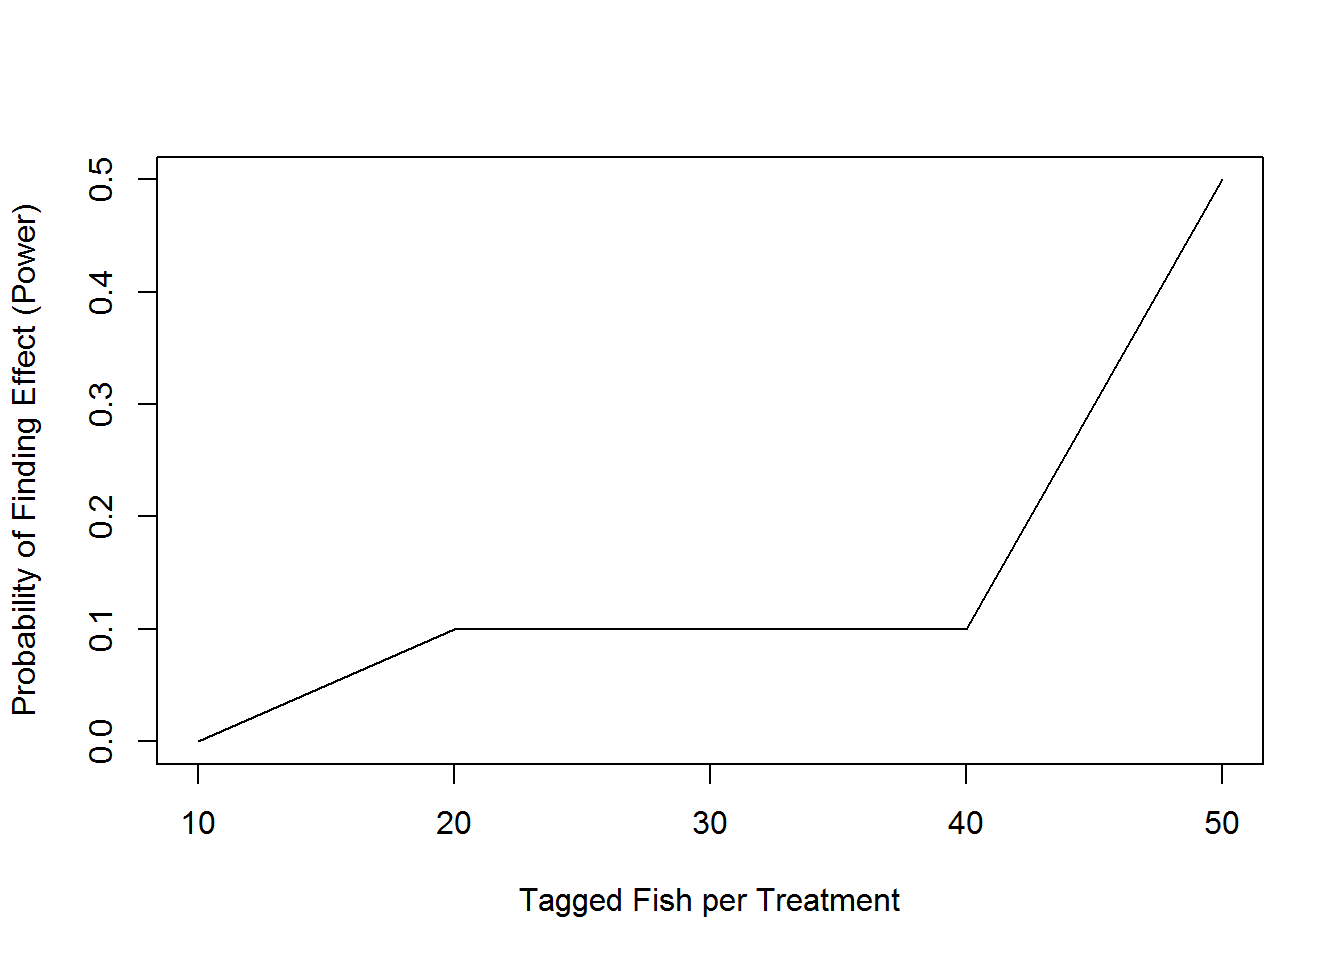
\includegraphics{au-r-workshop_files/figure-latex/unnamed-chunk-171-1} \end{center}

The fact that all the quantiles fall around the 1:1 line sugggests the
\texttt{n} random samples samples are indeed from a normal distribution.
Any variabilities you see are due to sampling errors. If you increase
\texttt{n} to \texttt{n\ =\ 1e6} (one million), you'll see no
deviations. This is called a \textbf{q-q plot}, and is frequently used
to assess the fit of data to a distribution.

Now test the random values in their agreement with the \texttt{pnorm()}
function. Plot the cumulative density functions for the truely normal
curve and that approximated by the random deviates:

\begin{Shaded}
\begin{Highlighting}[]
\NormalTok{q =}\StringTok{ }\KeywordTok{seq}\NormalTok{(}\DecValTok{400}\NormalTok{, }\DecValTok{600}\NormalTok{, }\DecValTok{10}\NormalTok{)}
\NormalTok{random_cdf =}\StringTok{ }\KeywordTok{ecdf}\NormalTok{(random)}
\NormalTok{random_p =}\StringTok{ }\KeywordTok{random_cdf}\NormalTok{(q)}
\NormalTok{normal_p =}\StringTok{ }\KeywordTok{pnorm}\NormalTok{(q, mu, sig)}
\KeywordTok{plot}\NormalTok{(normal_p }\OperatorTok{~}\StringTok{ }\NormalTok{q, }\DataTypeTok{type =} \StringTok{"l"}\NormalTok{, }\DataTypeTok{col =} \StringTok{"blue"}\NormalTok{)}
\KeywordTok{points}\NormalTok{(random_p }\OperatorTok{~}\StringTok{ }\NormalTok{q, }\DataTypeTok{col =} \StringTok{"red"}\NormalTok{)}
\end{Highlighting}
\end{Shaded}

\begin{center}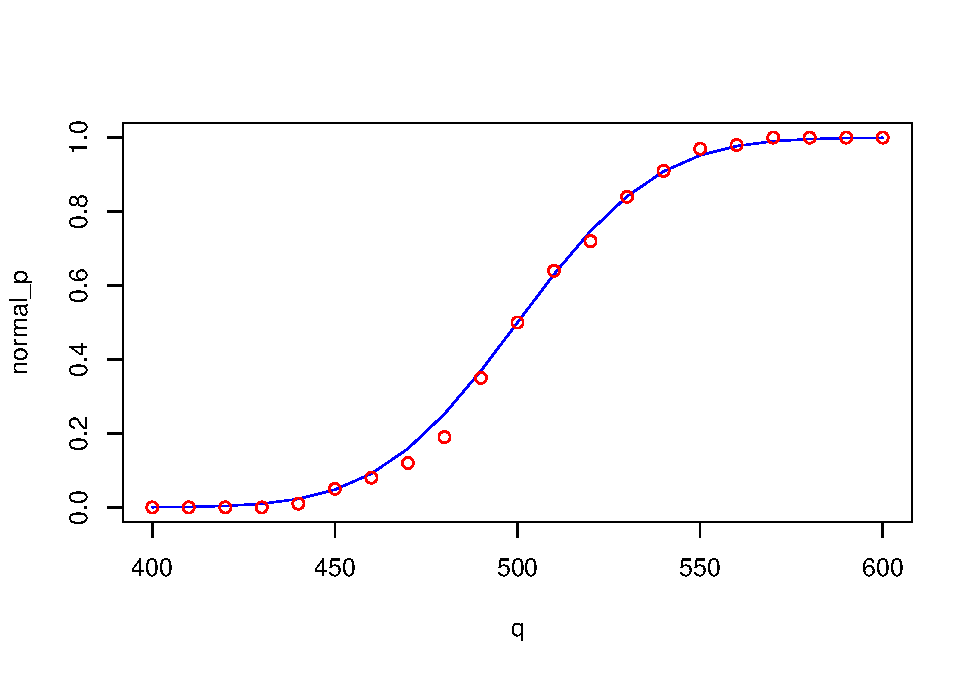
\includegraphics{au-r-workshop_files/figure-latex/unnamed-chunk-172-1} \end{center}

The \texttt{ecdf()} function obtains the empirical cumulative density
function (which is just \texttt{pnorm()} for a sample). It allows you to
plug in any random variable and obtain the probability of having one
less than it.

\subsection{Stochastic Power Analysis}\label{power-ex}

A \textbf{power analysis} is one where the analyst wishes to determine
how much power they will have to detect an effect. Having high power
means ensuring you do not falsely reject a true hypothesis (e.g.,
claiming that there is no effect based on a p-value greater than 0.05
when there truly is an effect).

You can conduct a power analysis using stochastic simulation (i.e., a
Monte Carlo analysis). Here, you will write a power analysis to
determine how likely are you to be able to correctly identify what you
deem to be a biologically-meaningful difference in survival between two
tagging procedures. You know one tagging procedure has approximately a
10\% mortality rate (10\% of tagged fish die within the first 12 hours
as result of the tagging process). Another, cheaper and less
labor-intensive method has been proposed but before implementing it,
your agency wishes to determine if it will have a meaningful impact on
the reliability of the study or the efficiency of the tagging crew to
tag individuals that will be alive long enough to be useful. You and
your colleagues determine that if the mortality rate of the new tagging
method reaches 25\%, then gains in time and cost efficiency would be
offset by needing to tag more fish (because more will die). You have
decided to perform a small-scale study to determine if the new method
affects mortality enough to result in 25\% or more mortality. The study
will tag \texttt{n} individuals using each method (new and old) and
track the fraction that survived after 12 hours. Before performing the
study however, you deem it important to determine how large \texttt{n}
needs to be to answer this question. You decide to use a stochastic
power analysis based on what you've learned in this book to help your
research group. The small-scale study can tag a total of at most 100
fish with the currently available resources. Could you tag fewer than
100 total individuals and still have a high probability of correctly
identifying an effect of this size?

The stochastic power analysis approach works like this (this is called
\textbf{psuedocode}):

\begin{enumerate}
\def\labelenumi{\arabic{enumi}.}
\tightlist
\item
  Simulate data under the reality that the difference is real with
  \texttt{n} observations per treatment, where
  \texttt{n\ \textless{}\ 100/2}
\item
  Fit the model that will be used when the real data are collected to
  the simulated data
\item
  Determine if the effect was detected with a significant p-value
\item
  Replicate steps 1 - 3 many times
\item
  Replicate step 4 while varying \texttt{n} over the interval from 10 to
  50
\item
  Determine what fraction of the p-values were deemed significant at
  each \texttt{n}
\end{enumerate}

Step 2 will require fitting a generalized linear model, for a review
revisit Section \ref{glms} (specifically Section \ref{logis-regression}
on logistic regression).

First, create a function that will generate data, fit the model, and
determine if the p-value is significant (steps 1-3 above):

\begin{Shaded}
\begin{Highlighting}[]
\NormalTok{sim_fit =}\StringTok{ }\ControlFlowTok{function}\NormalTok{(n, }\DataTypeTok{p_old =} \FloatTok{0.10}\NormalTok{, }\DataTypeTok{p_new =} \FloatTok{0.25}\NormalTok{) \{}
  
\NormalTok{  ### step 1: create the data }\AlertTok{###}
  \CommentTok{# generate random response data}
\NormalTok{  dead_old =}\StringTok{ }\KeywordTok{rbinom}\NormalTok{(n, }\DataTypeTok{size =} \DecValTok{1}\NormalTok{, }\DataTypeTok{prob =}\NormalTok{ p_old)}
\NormalTok{  dead_new =}\StringTok{ }\KeywordTok{rbinom}\NormalTok{(n, }\DataTypeTok{size =} \DecValTok{1}\NormalTok{, }\DataTypeTok{prob =}\NormalTok{ p_new)}
  \CommentTok{# create the predictor variable}
\NormalTok{  method =}\StringTok{ }\KeywordTok{rep}\NormalTok{(}\KeywordTok{c}\NormalTok{(}\StringTok{"old"}\NormalTok{, }\StringTok{"new"}\NormalTok{), }\DataTypeTok{each =}\NormalTok{ n)}
  \CommentTok{# create a data.frame to pass to glm}
\NormalTok{  df =}\StringTok{ }\KeywordTok{data.frame}\NormalTok{(}\DataTypeTok{dead =} \KeywordTok{c}\NormalTok{(dead_old, dead_new), }\DataTypeTok{method =}\NormalTok{ method)}
  \CommentTok{# relevel so old is the reference}
\NormalTok{  df}\OperatorTok{$}\NormalTok{method =}\StringTok{ }\KeywordTok{relevel}\NormalTok{(df}\OperatorTok{$}\NormalTok{method, }\DataTypeTok{ref =} \StringTok{"old"}\NormalTok{)}
  
\NormalTok{  ### step 2: fit the model }\AlertTok{###}
\NormalTok{  fit =}\StringTok{ }\KeywordTok{glm}\NormalTok{(dead }\OperatorTok{~}\StringTok{ }\NormalTok{method, }\DataTypeTok{data =}\NormalTok{ df, }\DataTypeTok{family =}\NormalTok{ binomial)}
  
\NormalTok{  ### step 3: determine if a sig. p-value was found }\AlertTok{###}
  \CommentTok{# extract the p-value}
\NormalTok{  pval =}\StringTok{ }\KeywordTok{summary}\NormalTok{(fit)}\OperatorTok{$}\NormalTok{coef[}\DecValTok{2}\NormalTok{,}\DecValTok{4}\NormalTok{]}
  \CommentTok{# determine if it was found to be significant}
\NormalTok{  pval }\OperatorTok{<}\StringTok{ }\FloatTok{0.05}
\NormalTok{\}}
\end{Highlighting}
\end{Shaded}

Next, for steps 4 and 5, set up a \textbf{nested \texttt{for} loop}.
This will have two loops: one that loops over sample sizes for step 5
and one that loops over replicates of each sample size (step 4):

\begin{Shaded}
\begin{Highlighting}[]
\NormalTok{I =}\StringTok{ }\DecValTok{500}  \CommentTok{# the number of replicates at each sample size}
\NormalTok{n_try =}\StringTok{ }\KeywordTok{seq}\NormalTok{(}\DecValTok{10}\NormalTok{, }\DecValTok{50}\NormalTok{, }\DecValTok{10}\NormalTok{)  }\CommentTok{# the test sample sizes}
\NormalTok{N =}\StringTok{ }\KeywordTok{length}\NormalTok{(n_try)        }\CommentTok{# count them}
\CommentTok{# container: }
\NormalTok{out =}\StringTok{ }\KeywordTok{matrix}\NormalTok{(}\OtherTok{NA}\NormalTok{, I, N) }\CommentTok{# matrix with I rows and N columns}
\ControlFlowTok{for}\NormalTok{ (n }\ControlFlowTok{in} \DecValTok{1}\OperatorTok{:}\NormalTok{N) \{}
  \ControlFlowTok{for}\NormalTok{ (i }\ControlFlowTok{in} \DecValTok{1}\OperatorTok{:}\NormalTok{I) \{}
\NormalTok{    out[i,n] =}\StringTok{ }\KeywordTok{sim_fit}\NormalTok{(}\DataTypeTok{n =}\NormalTok{ n_try[n])}
\NormalTok{  \}}
\NormalTok{\}}
\end{Highlighting}
\end{Shaded}

You now have a matrix of \texttt{TRUE} and \texttt{FALSE} elements that
indicates whether a significant difference was found at the
\(\alpha = 0.05\) level if the effect was truely as large as you care
about. You can obtain the proportion of all the replicates at each
sample size that resulted in a significant difference using the
\texttt{mean} function with \texttt{apply}:

\begin{Shaded}
\begin{Highlighting}[]
\KeywordTok{plot}\NormalTok{(}\KeywordTok{apply}\NormalTok{(out, }\DecValTok{2}\NormalTok{, mean) }\OperatorTok{~}\StringTok{ }\NormalTok{n_try, }\DataTypeTok{type =} \StringTok{"l"}\NormalTok{,}
     \DataTypeTok{xlab =} \StringTok{"Tagged Fish per Treatment"}\NormalTok{,}
     \DataTypeTok{ylab =} \StringTok{"Probability of Finding Effect (Power)"}\NormalTok{)}
\end{Highlighting}
\end{Shaded}

\begin{center}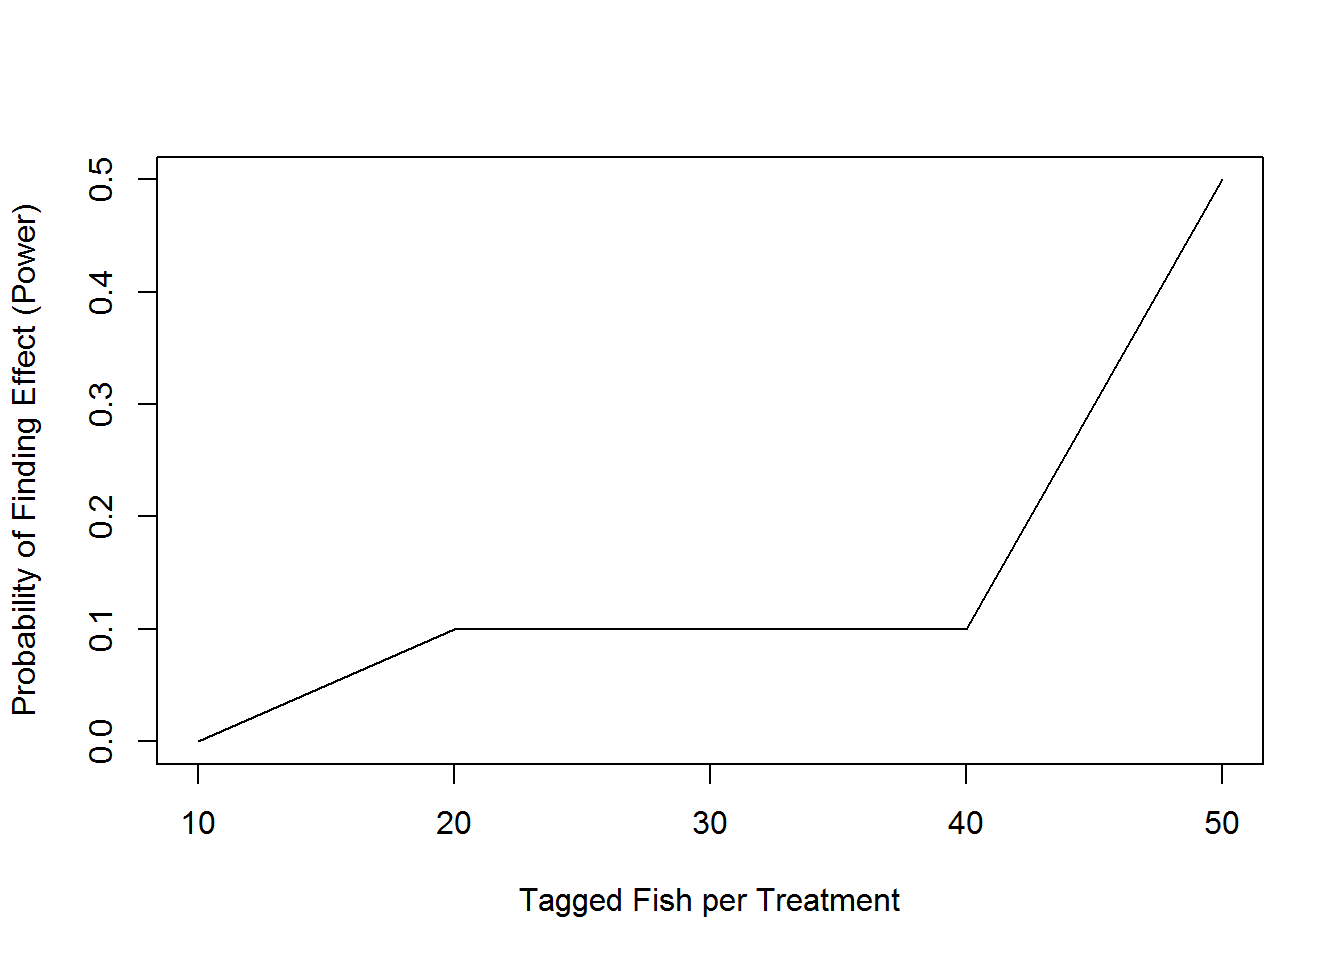
\includegraphics{au-r-workshop_files/figure-latex/unnamed-chunk-175-1} \end{center}

Even if you tagged 100 fish total, you would only have a 47\% chance of
saying the effect (which truely is there!) is present under the null
hypothesis testing framework.

Suppose you and your colleagues aren't relying on p-values in this case,
and are purely interested in how precisely the \textbf{effect size}
would be estimated. Adapt your function to determine how frequently it
is you would be able to estimate the true mortality probability of the
new method within +/- 5\% based on the point estimate only (the estimate
for the tagging mortality of the new method must be between 0.2 and 0.3
for a successful study). Change your function to calculate this
additional metric and re-run the analysis:

\begin{Shaded}
\begin{Highlighting}[]
\NormalTok{sim_fit =}\StringTok{ }\ControlFlowTok{function}\NormalTok{(n, }\DataTypeTok{p_old =} \FloatTok{0.10}\NormalTok{, }\DataTypeTok{p_new =} \FloatTok{0.25}\NormalTok{) \{}
  \CommentTok{# create the data}
\NormalTok{  dead_old =}\StringTok{ }\KeywordTok{rbinom}\NormalTok{(n, }\DataTypeTok{size =} \DecValTok{1}\NormalTok{, }\DataTypeTok{prob =}\NormalTok{ p_old)}
\NormalTok{  dead_new =}\StringTok{ }\KeywordTok{rbinom}\NormalTok{(n, }\DataTypeTok{size =} \DecValTok{1}\NormalTok{, }\DataTypeTok{prob =}\NormalTok{ p_new)}
  \CommentTok{# create the predictor variable}
\NormalTok{  method =}\StringTok{ }\KeywordTok{rep}\NormalTok{(}\KeywordTok{c}\NormalTok{(}\StringTok{"old"}\NormalTok{, }\StringTok{"new"}\NormalTok{), }\DataTypeTok{each =}\NormalTok{ n)}
  \CommentTok{# create a data.frame to pass to glm}
\NormalTok{  df =}\StringTok{ }\KeywordTok{data.frame}\NormalTok{(}\DataTypeTok{dead =} \KeywordTok{c}\NormalTok{(dead_old, dead_new), }\DataTypeTok{method =}\NormalTok{ method)}
  \CommentTok{# relevel so old is the reference}
\NormalTok{  df}\OperatorTok{$}\NormalTok{method =}\StringTok{ }\KeywordTok{relevel}\NormalTok{(df}\OperatorTok{$}\NormalTok{method, }\DataTypeTok{ref =} \StringTok{"old"}\NormalTok{)}
  \CommentTok{# fit the model}
\NormalTok{  fit =}\StringTok{ }\KeywordTok{glm}\NormalTok{(dead }\OperatorTok{~}\StringTok{ }\NormalTok{method, }\DataTypeTok{data =}\NormalTok{ df, }\DataTypeTok{family =}\NormalTok{ binomial)}
  \CommentTok{# extract the p-value}
\NormalTok{  pval =}\StringTok{ }\KeywordTok{summary}\NormalTok{(fit)}\OperatorTok{$}\NormalTok{coef[}\DecValTok{2}\NormalTok{,}\DecValTok{4}\NormalTok{]}
  \CommentTok{# determine if it was found to be significant}
\NormalTok{  sig_pval =}\StringTok{ }\NormalTok{pval }\OperatorTok{<}\StringTok{ }\FloatTok{0.05}
  \CommentTok{# obtain the estimated mortality rate for the new method}
\NormalTok{  p_new_est =}\StringTok{ }\KeywordTok{predict}\NormalTok{(fit, }\KeywordTok{data.frame}\NormalTok{(}\DataTypeTok{method =} \KeywordTok{c}\NormalTok{(}\StringTok{"new"}\NormalTok{)),}
                      \DataTypeTok{type =} \StringTok{"response"}\NormalTok{)}
  
  \CommentTok{# determine if it is +/- 5% from the true value}
\NormalTok{  prc_est =}\StringTok{ }\NormalTok{p_new_est }\OperatorTok{>=}\StringTok{ }\NormalTok{(p_new }\OperatorTok{-}\StringTok{ }\FloatTok{0.05}\NormalTok{) }\OperatorTok{&}\StringTok{ }\NormalTok{p_new_est }\OperatorTok{<=}\StringTok{ }\NormalTok{(p_new }\OperatorTok{+}\StringTok{ }\FloatTok{0.05}\NormalTok{)}
  \CommentTok{# return a vector with these two elements}
  \KeywordTok{c}\NormalTok{(}\DataTypeTok{sig_pval =}\NormalTok{ sig_pval, }\DataTypeTok{prc_est =} \KeywordTok{unname}\NormalTok{(prc_est))}
\NormalTok{\}}

\CommentTok{# run the analysis}
\NormalTok{I =}\StringTok{ }\DecValTok{500}  \CommentTok{# the number of replicates at each sample size}
\NormalTok{n_try =}\StringTok{ }\KeywordTok{seq}\NormalTok{(}\DecValTok{10}\NormalTok{, }\DecValTok{50}\NormalTok{, }\DecValTok{10}\NormalTok{)  }\CommentTok{# the test sample sizes}
\NormalTok{N =}\StringTok{ }\KeywordTok{length}\NormalTok{(n_try)      }\CommentTok{# count them}

\CommentTok{# containers: }
\NormalTok{out_sig =}\StringTok{ }\KeywordTok{matrix}\NormalTok{(}\OtherTok{NA}\NormalTok{, I, N) }\CommentTok{# matrix with I rows and N columns}
\NormalTok{out_prc =}\StringTok{ }\KeywordTok{matrix}\NormalTok{(}\OtherTok{NA}\NormalTok{, I, N) }\CommentTok{# matrix with I rows and N columns}
\ControlFlowTok{for}\NormalTok{ (n }\ControlFlowTok{in} \DecValTok{1}\OperatorTok{:}\NormalTok{N) \{}
  \ControlFlowTok{for}\NormalTok{ (i }\ControlFlowTok{in} \DecValTok{1}\OperatorTok{:}\NormalTok{I) \{}
\NormalTok{    tmp =}\StringTok{ }\KeywordTok{sim_fit}\NormalTok{(}\DataTypeTok{n =}\NormalTok{ n_try[n])     }\CommentTok{# run sim}
\NormalTok{    out_sig[i,n] =}\StringTok{ }\NormalTok{tmp[}\StringTok{"sig_pval"}\NormalTok{]  }\CommentTok{# extract and store significance metric}
\NormalTok{    out_prc[i,n] =}\StringTok{ }\NormalTok{tmp[}\StringTok{"prc_est"}\NormalTok{]   }\CommentTok{# extract and store precision metric}
\NormalTok{  \}}
\NormalTok{\}}

\KeywordTok{par}\NormalTok{(}\DataTypeTok{mfrow =} \KeywordTok{c}\NormalTok{(}\DecValTok{1}\NormalTok{,}\DecValTok{2}\NormalTok{))}
\KeywordTok{plot}\NormalTok{(}\KeywordTok{apply}\NormalTok{(out_sig, }\DecValTok{2}\NormalTok{, mean) }\OperatorTok{~}\StringTok{ }\NormalTok{n_try, }\DataTypeTok{type =} \StringTok{"l"}\NormalTok{,}
     \DataTypeTok{xlab =} \StringTok{"Tagged Fish per Treatment"}\NormalTok{,}
     \DataTypeTok{ylab =} \StringTok{"Probability of Finding Effect (Power)"}\NormalTok{)}
\KeywordTok{plot}\NormalTok{(}\KeywordTok{apply}\NormalTok{(out_prc, }\DecValTok{2}\NormalTok{, mean) }\OperatorTok{~}\StringTok{ }\NormalTok{n_try, }\DataTypeTok{type =} \StringTok{"l"}\NormalTok{,}
     \DataTypeTok{xlab =} \StringTok{"Tagged Fish per Treatment"}\NormalTok{,}
     \DataTypeTok{ylab =} \StringTok{"Probability of A Precise Estimate"}\NormalTok{)}
\end{Highlighting}
\end{Shaded}

\begin{center}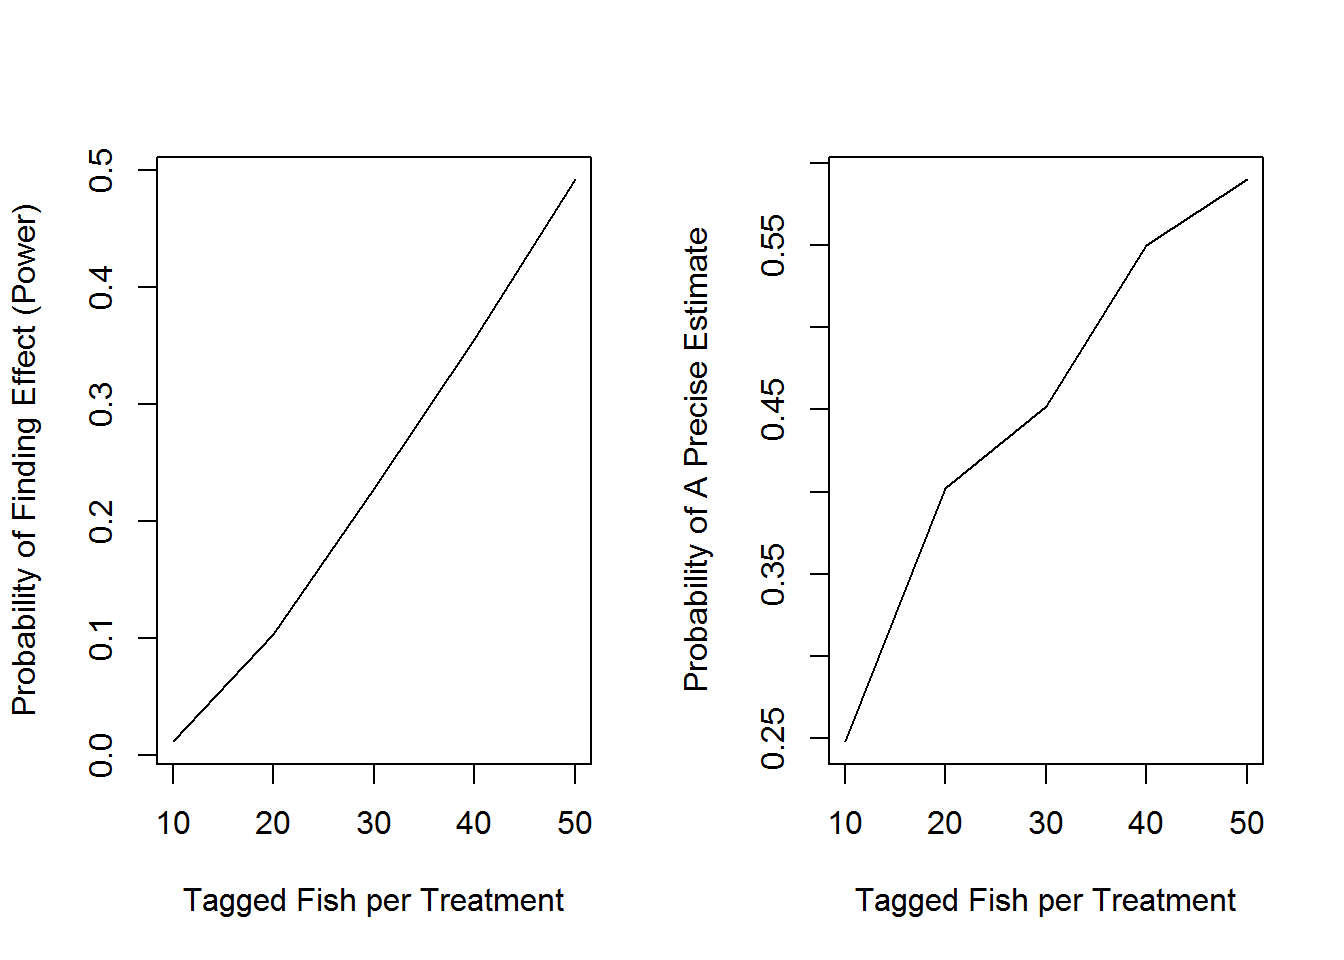
\includegraphics{au-r-workshop_files/figure-latex/unnamed-chunk-176-1} \end{center}

It seems that even if you tagged 50 fish per treatment, you would have a
59\% chance of estimating that the mortality rate is between 0.2 and 0.3
if it was truly 0.25.

You and your colleagues consider these results and determine that you
will need to somehow acquire more funds to tag more fish in the
small-scale study in order to a high level of confidence in the results.

\subsection{Harvest Policy Analysis}\label{harv-ex}

In this example, you will simulate population dynamics under a more
realistic model than in Sections \ref{for-loops} and \ref{adv-funcs} for
the purpose of evaluating different harvest policies.

Suppose you are a fisheries research biologist, and a commercial fishery
for pink salmon (\emph{Oncorhynchus gorbuscha}) takes place in your
district. For the past 10 years, it has been fished with an exploitation
rate of 40\% (40\% of the fish that return each year have been
harvested, exploitation rate is abbreviated by \(U\)), resulting in an
average annual harvest of 8.5 million fish. The management plan is up
for evaluation this year, and your supervisor has asked you to prepare
an analysis that determines if more harvest could be sustained if a
different exploitation rate were to be used in the future.

Based on historical data, your best understanding implies that the stock
is driven by Ricker spawner-recruit dynamics. That is, the total number
of fish that return this year (recruits) are a function of the total
number of spawners that produced and fertilized the eggs from which this
year's recruits were produced. The Ricker model can be written this way:

\begin{equation}
  R_t = \alpha S_{t-1} e^{-\beta S_{t-1} + \varepsilon_t} ,\varepsilon_t \sim N(0,\sigma)
\label{eq:ricker-ch4}
\end{equation}

where \(\alpha\) is a parameter representing the maximum recruits per
spawner (obtained at very low spawner abundances) and \(\beta\) is a
measure of the strength of density-dependent mortality. Notice that the
error term is in the exponent, which makes \(e^{\varepsilon_t}\)
lognormal.

You have estimates of the parameters\footnote{In reality, these
  estimates would have substantial uncertainty that you would need to
  propogate through your harvest policy analysis. In this example, you
  will ignore this complication}:

\begin{itemize}
\tightlist
\item
  \(\alpha = 6\)
\item
  \(\beta = 1 \times 10^{-7}\)
\item
  \(\sigma = 0.4\)
\end{itemize}

You decide that you can build a policy analysis by simulating the stock
forward through time under different exploitation rates to determine if
its reasonable to expect a different exploitation rate to provide more
harvest than what is currently being extracted.

First, write a function for your population model. Your function must:

\begin{enumerate}
\def\labelenumi{\arabic{enumi}.}
\tightlist
\item
  take the parameters, dimensions (number of years), and the policy
  variable (\(U\)) as input arguments
\item
  simulate the population using Ricker dynamics
\item
  calculate and return the average harvest and escapement over the
  number future years you simulated.
\end{enumerate}

\begin{Shaded}
\begin{Highlighting}[]
\CommentTok{# Step #1: name function and give it some arguments}
\NormalTok{ricker_sim =}\StringTok{ }\ControlFlowTok{function}\NormalTok{(ny, params, U) \{}
  \CommentTok{# extract the parameters out by name:}
\NormalTok{  alpha =}\StringTok{ }\NormalTok{params[}\StringTok{"alpha"}\NormalTok{]}
\NormalTok{  beta =}\StringTok{ }\NormalTok{params[}\StringTok{"beta"}\NormalTok{]}
\NormalTok{  sigma =}\StringTok{ }\NormalTok{params[}\StringTok{"sigma"}\NormalTok{]}
  \CommentTok{# create containers:}
  \CommentTok{# yep, you can do this}
\NormalTok{  R =}\StringTok{ }\NormalTok{S =}\StringTok{ }\NormalTok{H =}\StringTok{ }\OtherTok{NULL}
  \CommentTok{# initialize the population in the first year}
    \CommentTok{# start the population at being fished at 40%}
    \CommentTok{# with lognormal error}
\NormalTok{  R[}\DecValTok{1}\NormalTok{] =}\StringTok{ }\KeywordTok{log}\NormalTok{(alpha }\OperatorTok{*}\StringTok{ }\NormalTok{(}\DecValTok{1} \OperatorTok{-}\StringTok{ }\FloatTok{0.4}\NormalTok{))}\OperatorTok{/}\NormalTok{(beta }\OperatorTok{*}\StringTok{ }\NormalTok{(}\DecValTok{1} \OperatorTok{-}\StringTok{ }\FloatTok{0.4}\NormalTok{)) }\OperatorTok{*}\StringTok{ }\KeywordTok{exp}\NormalTok{(}\KeywordTok{rnorm}\NormalTok{(}\DecValTok{1}\NormalTok{, }\DecValTok{0}\NormalTok{, sigma))}
\NormalTok{  S[}\DecValTok{1}\NormalTok{] =}\StringTok{ }\NormalTok{R[}\DecValTok{1}\NormalTok{] }\OperatorTok{*}\StringTok{ }\NormalTok{(}\DecValTok{1} \OperatorTok{-}\StringTok{ }\NormalTok{U)}
\NormalTok{  H[}\DecValTok{1}\NormalTok{] =}\StringTok{ }\NormalTok{R[}\DecValTok{1}\NormalTok{] }\OperatorTok{*}\StringTok{ }\NormalTok{U}
  
  \CommentTok{# carry simulation forward through time}
  \ControlFlowTok{for}\NormalTok{ (y }\ControlFlowTok{in} \DecValTok{2}\OperatorTok{:}\NormalTok{ny) \{}
    \CommentTok{# use the ricker function with random lognormal white noise}
\NormalTok{    R[y] =}\StringTok{ }\NormalTok{S[y}\OperatorTok{-}\DecValTok{1}\NormalTok{] }\OperatorTok{*}\StringTok{ }\NormalTok{alpha }\OperatorTok{*}\StringTok{ }\KeywordTok{exp}\NormalTok{(}\OperatorTok{-}\NormalTok{beta }\OperatorTok{*}\StringTok{ }\NormalTok{S[y}\OperatorTok{-}\DecValTok{1}\NormalTok{] }\OperatorTok{+}\StringTok{ }\KeywordTok{rnorm}\NormalTok{(}\DecValTok{1}\NormalTok{, }\DecValTok{0}\NormalTok{, sigma))}
    \CommentTok{#harvest and spawners are the same as before}
\NormalTok{    S[y] =}\StringTok{ }\NormalTok{R[y] }\OperatorTok{*}\StringTok{ }\NormalTok{(}\DecValTok{1} \OperatorTok{-}\StringTok{ }\NormalTok{U)}
\NormalTok{    H[y] =}\StringTok{ }\NormalTok{R[y] }\OperatorTok{*}\StringTok{ }\NormalTok{U}
\NormalTok{  \}}
  \CommentTok{# wrap output in a list object}
  \KeywordTok{list}\NormalTok{(}
    \DataTypeTok{mean_H =} \KeywordTok{mean}\NormalTok{(H),}
    \DataTypeTok{mean_S =} \KeywordTok{mean}\NormalTok{(S)}
\NormalTok{    )}
\NormalTok{\}}
\end{Highlighting}
\end{Shaded}

Use the function once:

\begin{Shaded}
\begin{Highlighting}[]
\NormalTok{params =}\StringTok{ }\KeywordTok{c}\NormalTok{(}\DataTypeTok{alpha =} \DecValTok{6}\NormalTok{, }\DataTypeTok{beta =} \FloatTok{1e-7}\NormalTok{, }\DataTypeTok{sigma =} \FloatTok{0.4}\NormalTok{)}
\NormalTok{out =}\StringTok{ }\KeywordTok{ricker_sim}\NormalTok{(}\DataTypeTok{U =} \FloatTok{0.4}\NormalTok{, }\DataTypeTok{ny =} \DecValTok{20}\NormalTok{, }\DataTypeTok{params =}\NormalTok{ params)}
\CommentTok{#average annual harvest (in millions)}
\KeywordTok{round}\NormalTok{(out}\OperatorTok{$}\NormalTok{mean_H}\OperatorTok{/}\FloatTok{1e6}\NormalTok{, }\DataTypeTok{digits =} \DecValTok{2}\NormalTok{)}
\end{Highlighting}
\end{Shaded}

\begin{verbatim}
## [1] 8.52
\end{verbatim}

If you completed the stochastic power analysis example (Section
\ref{power-ex}), you might see where this is going. You are going to
replicate applying a fixed policy many times to a random system. This is
the Monte Carlo part of the analysis. The policy part is that you will
compare the output from several candidate exploitation rates to inform a
decision about which is best. This time, set up your analysis using
\texttt{sapply()} (to iterate over different values of \(U\)) and
\texttt{replicate()} (to iterate over different random populations
fished at each \(U\)) instead of performing a nested \texttt{for()} loop
as in previous examples:

\begin{Shaded}
\begin{Highlighting}[]
\NormalTok{U_try =}\StringTok{ }\KeywordTok{seq}\NormalTok{(}\FloatTok{0.4}\NormalTok{, }\FloatTok{0.6}\NormalTok{, }\FloatTok{0.01}\NormalTok{)}
\NormalTok{n_rep =}\StringTok{ }\DecValTok{500}
\NormalTok{H_out =}\StringTok{ }\KeywordTok{sapply}\NormalTok{(U_try, }\ControlFlowTok{function}\NormalTok{(u) \{}
  \KeywordTok{replicate}\NormalTok{(}\DataTypeTok{n =}\NormalTok{ n_rep, }\DataTypeTok{expr =}\NormalTok{ \{}
    \KeywordTok{ricker_sim}\NormalTok{(}\DataTypeTok{U =}\NormalTok{ u, }\DataTypeTok{ny =} \DecValTok{20}\NormalTok{, }\DataTypeTok{params =}\NormalTok{ params)}\OperatorTok{$}\NormalTok{mean_H}\OperatorTok{/}\FloatTok{1e6}
\NormalTok{  \})}
\NormalTok{\})}
\end{Highlighting}
\end{Shaded}

The nested \texttt{replicate()} and \texttt{sapply()} method is a bit
cleaner than a nested \texttt{for()} loop, but you have less control
over the format of the output.

Plot the output of your simulations using a boxplot. To make things
easier, give \texttt{H\_out} column names representing the exploitation
rate:

\begin{Shaded}
\begin{Highlighting}[]
\KeywordTok{colnames}\NormalTok{(H_out) =}\StringTok{ }\NormalTok{U_try}
\KeywordTok{boxplot}\NormalTok{(H_out, }\DataTypeTok{outline =}\NormalTok{ F,}
        \DataTypeTok{xlab =} \StringTok{"U"}\NormalTok{, }\DataTypeTok{ylab =} \StringTok{"Harvest (Millions of Fish)"}\NormalTok{,}
        \DataTypeTok{col =} \StringTok{"tomato"}\NormalTok{, }\DataTypeTok{las =} \DecValTok{1}\NormalTok{)}
\end{Highlighting}
\end{Shaded}

\begin{center}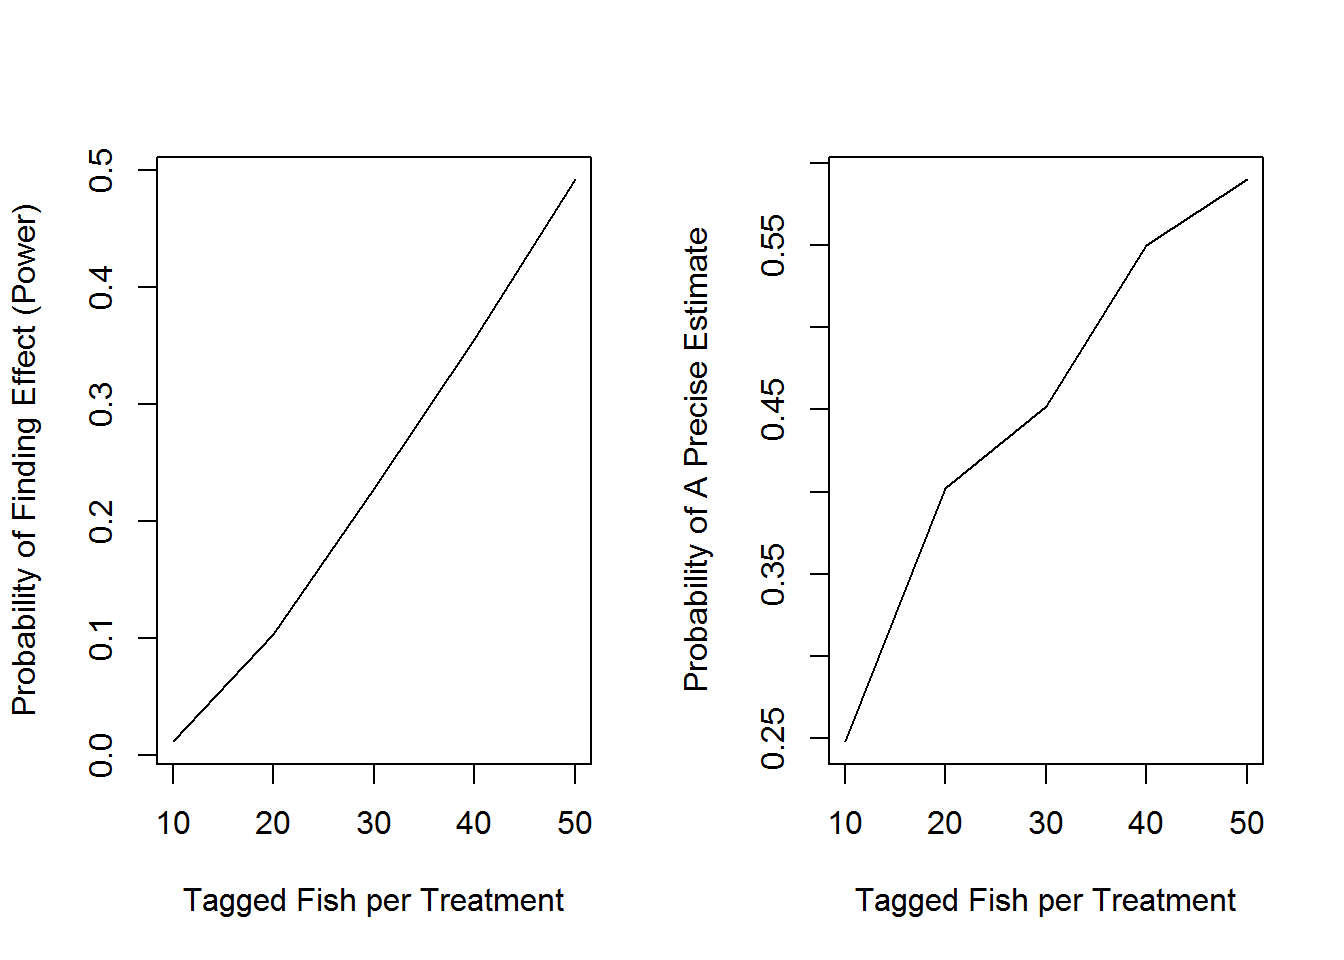
\includegraphics{au-r-workshop_files/figure-latex/unnamed-chunk-180-1} \end{center}

It appears the stock could produce more harvest than its current 8.5
million fish per year if it was fished harder. However, your supervisors
also do not want to see the escapement drop below three-quarters of what
it has been in recent history (75\% of approximately 13 million fish).
They ask you to obtain the expected average annual escapement as well as
harvest. You can simply re-run the code above, but extracting
\texttt{S\_mean} rather than \texttt{H\_mean}. Call this output
\texttt{S\_out} and plot it just like harvest (if you're curious, this
blue color is \texttt{col\ =\ "skyblue"}):

\begin{center}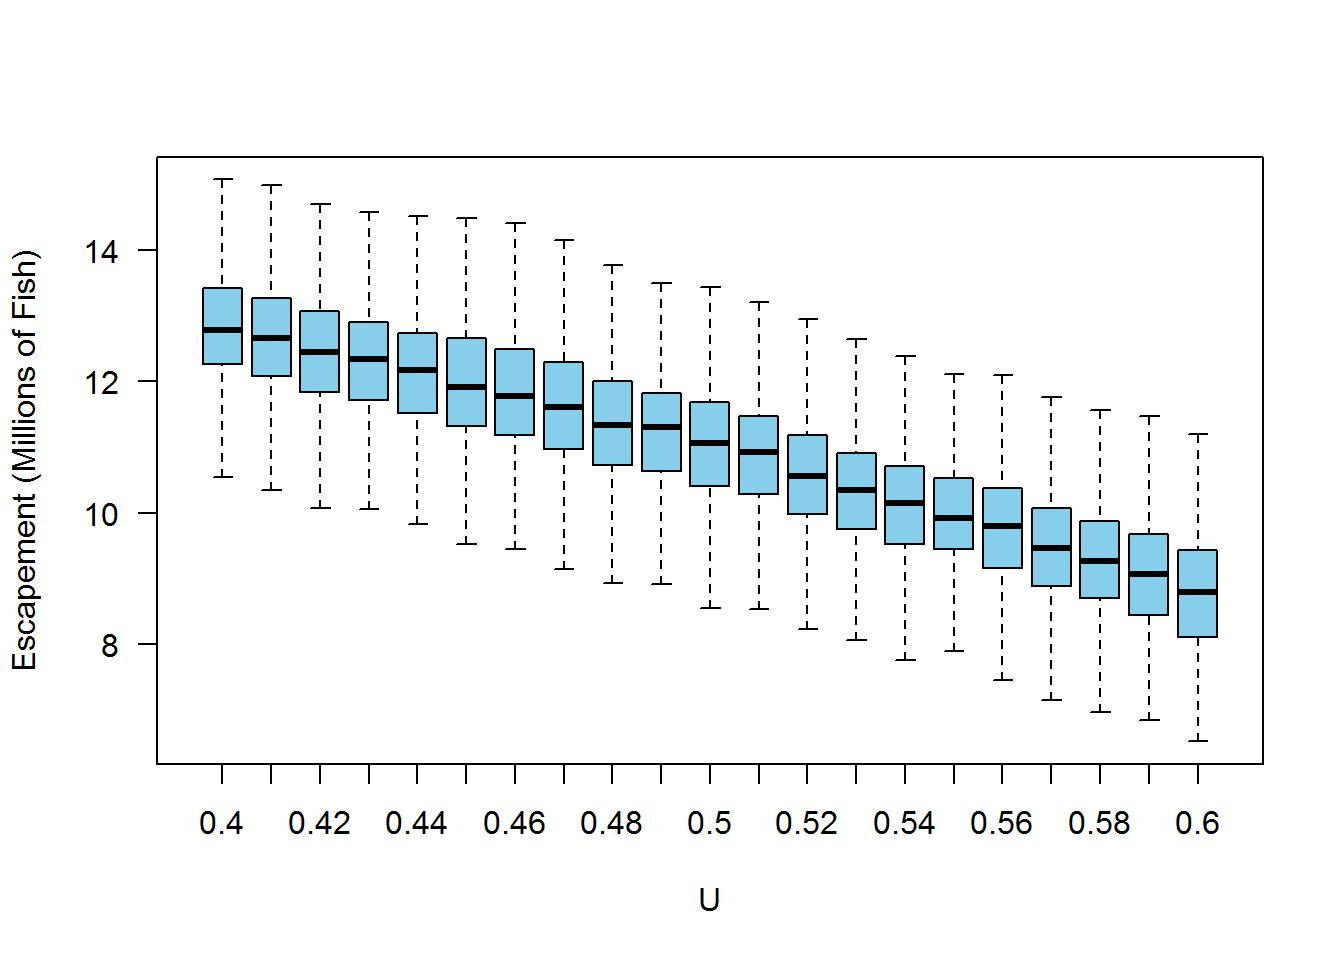
\includegraphics{au-r-workshop_files/figure-latex/unnamed-chunk-181-1} \end{center}

After seeing this information, your supervisor realizes they are faced
with a trade-off: the stock could produce more with high exploitation
rates, but they are concerned about pushing the stock too low for
sustainability reasons. They tell you to determine the probability the
average escapement would not be pushed below 75\% of 13 million at each
exploitation rate, as well as the probability that the average annual
harvests will be at least 20\% greater than they are currently
(approximately 8.5 million fish). Given your output, this is easy:

\begin{Shaded}
\begin{Highlighting}[]
\CommentTok{# determine if each element meets escapement criterion}
\NormalTok{Smeet =}\StringTok{ }\NormalTok{S_out }\OperatorTok{>}\StringTok{ }\NormalTok{(}\FloatTok{0.75} \OperatorTok{*}\StringTok{ }\DecValTok{13}\NormalTok{)}
\CommentTok{# determine if each element meets harvest criterion}
\NormalTok{Hmeet =}\StringTok{ }\NormalTok{H_out }\OperatorTok{>}\StringTok{ }\NormalTok{(}\FloatTok{1.2} \OperatorTok{*}\StringTok{ }\FloatTok{8.5}\NormalTok{)}
\CommentTok{# calculate the probability of each occuring at a given exploitation rate}
  \CommentTok{# remember, mean of a logical vector calculate the proportion of TRUEs}
\NormalTok{p_Smeet =}\StringTok{ }\KeywordTok{apply}\NormalTok{(Smeet, }\DecValTok{2}\NormalTok{, mean)}
\NormalTok{p_Hmeet =}\StringTok{ }\KeywordTok{apply}\NormalTok{(Hmeet, }\DecValTok{2}\NormalTok{, mean)}
\end{Highlighting}
\end{Shaded}

You plot this for your supervisor as follows:

\begin{Shaded}
\begin{Highlighting}[]
\CommentTok{# the U levels to highlight on plot}
\NormalTok{plot_U =}\StringTok{ }\KeywordTok{seq}\NormalTok{(}\FloatTok{0.4}\NormalTok{, }\FloatTok{0.6}\NormalTok{, }\FloatTok{0.05}\NormalTok{)}
\CommentTok{# create an empty plot}
\KeywordTok{par}\NormalTok{(}\DataTypeTok{mar =} \KeywordTok{c}\NormalTok{(}\DecValTok{4}\NormalTok{,}\DecValTok{5}\NormalTok{,}\DecValTok{1}\NormalTok{,}\DecValTok{1}\NormalTok{))}
\KeywordTok{plot}\NormalTok{(p_Smeet }\OperatorTok{~}\StringTok{ }\NormalTok{p_Hmeet, }\DataTypeTok{type =} \StringTok{"n"}\NormalTok{,}
     \DataTypeTok{xlab =} \StringTok{"Probability of Meeting Harvest Criterion"}\NormalTok{,}
     \DataTypeTok{ylab =} \StringTok{"Probability of Meeting Escapement Criterion"}\NormalTok{)}
\CommentTok{# add gridlines}
\KeywordTok{abline}\NormalTok{(}\DataTypeTok{v =} \KeywordTok{seq}\NormalTok{(}\DecValTok{0}\NormalTok{, }\DecValTok{1}\NormalTok{, }\FloatTok{0.1}\NormalTok{), }\DataTypeTok{col =} \StringTok{"grey"}\NormalTok{)}
\KeywordTok{abline}\NormalTok{(}\DataTypeTok{h =} \KeywordTok{seq}\NormalTok{(}\DecValTok{0}\NormalTok{, }\DecValTok{1}\NormalTok{, }\FloatTok{0.1}\NormalTok{), }\DataTypeTok{col =} \StringTok{"grey"}\NormalTok{)}
\CommentTok{#draw on the tradeoff curve}
\KeywordTok{lines}\NormalTok{(p_Smeet }\OperatorTok{~}\StringTok{ }\NormalTok{p_Hmeet, }\DataTypeTok{type =} \StringTok{"l"}\NormalTok{, }\DataTypeTok{lwd =} \DecValTok{2}\NormalTok{)}
\CommentTok{# add points and text for particular U policies}
\KeywordTok{points}\NormalTok{(p_Smeet[U_try }\OperatorTok\StringTok{ }\NormalTok{plot_U] }\OperatorTok{~}\StringTok{ }\NormalTok{p_Hmeet[U_try }\OperatorTok\StringTok{ }\NormalTok{plot_U],}
       \DataTypeTok{pch =} \DecValTok{16}\NormalTok{, }\DataTypeTok{cex =} \FloatTok{1.5}\NormalTok{)}
\KeywordTok{text}\NormalTok{(p_Smeet[U_try }\OperatorTok\StringTok{ }\NormalTok{plot_U] }\OperatorTok{~}\StringTok{ }\NormalTok{p_Hmeet[U_try }\OperatorTok\StringTok{ }\NormalTok{plot_U],}
     \DataTypeTok{labels =}\NormalTok{ U_try[U_try }\OperatorTok\StringTok{ }\NormalTok{plot_U], }\DataTypeTok{pos =} \KeywordTok{c}\NormalTok{(}\DecValTok{1}\NormalTok{,}\DecValTok{1}\NormalTok{,}\DecValTok{1}\NormalTok{,}\DecValTok{2}\NormalTok{,}\DecValTok{2}\NormalTok{))}
\end{Highlighting}
\end{Shaded}

\begin{center}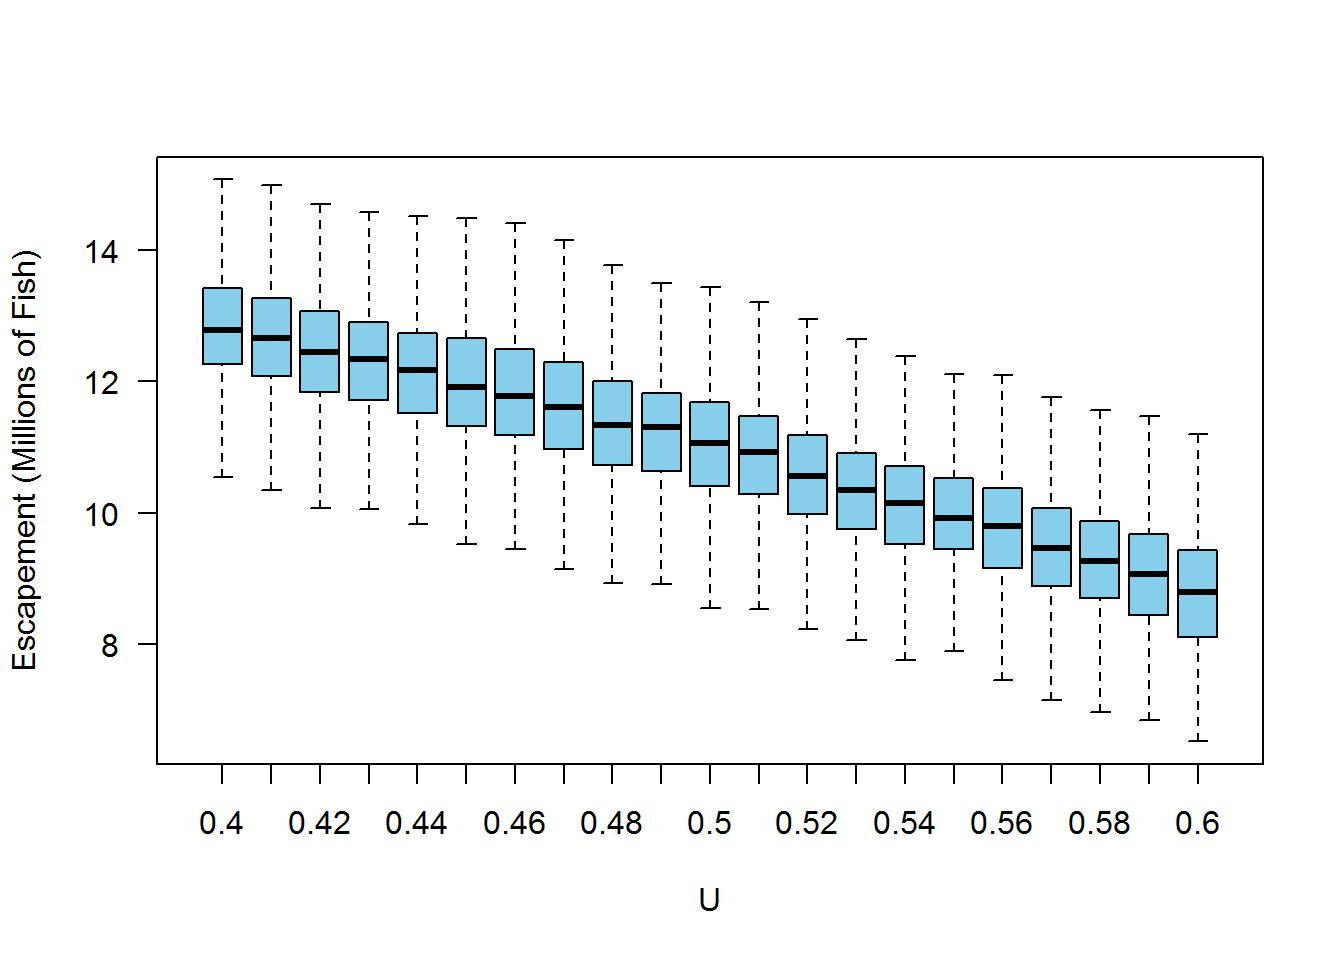
\includegraphics{au-r-workshop_files/figure-latex/unnamed-chunk-183-1} \end{center}

Equipped with this analysis, your supervisor plans to go to the
policy-makers with the recommendation of adjusting the exploitation rate
policy to use \(U = 0.5\), because they think it balances the trade-off.
Notice how if the status quo was maintained, your model suggests you
would have complete certainty of staying where you are now: escapement
will remain above 75\% of its current level with a 100\% chance, but you
would have no chance of improving harvests to greater than 20\% of their
current level. Small increases in the exploitation rate (e.g., from 0.4
to 0.45) have a reasonably large gain in harvest performance, but hardly
any losses for the escapement criterion. Your supervisor is willing to
live with a 90\% chance that the escapement will stay where they desire
in order to gain a \textgreater{}80\% chance of obtaining the desired
amount of increases in harvest.

The utility of using Monte Carlo methods in this example is the ability
to calculate the probability of some event you are interested in. There
are analytical (i.e., not simulation-based) solutions to predict the
annual harvest and escapement from a fixed \(U\) from a population with
parameters \(\alpha\) and \(\beta\), but by incorporating randomness,
you were able to obtain the relative weights of outcomes other than the
expectation under the deterministic Ricker model, thereby allowing the
assignment of probabilities to meeting the two criteria.

\section{Resampling-Based Examples}\label{resample-examples}

\subsection{The Bootstrap}\label{boot-test-ex}

Oftentimes, you'll have a fitted model that you wish to propagate the
uncertainty from to some derived quantity. Consider the case of the
\textbf{von Bertalanffy growth model}. This is a non-linear model used
to predict the size of an organism (weight or length) based on its age.
The model can be written for a non-linear regression model (see Section
\ref{nls}) as:

\begin{equation}
  L_i = L_{\infty}\left(1 - e^{-k(age_i-t_0)}\right) + \varepsilon_i, \varepsilon_i \sim N(0, \sigma)
\label{eq:vonB}
\end{equation}

where \(L_i\) and \(age_i\) are the observed length and age of
individual \(i\), respectively, and \(L_{\infty}\), \(k\), and \(t_0\)
are parameters to be estimated. The interpretations of the parameters
are as follows:

\begin{itemize}
\tightlist
\item
  \(L_{\infty}\): the maximum average length acheived
\item
  \(k\): a growth coefficient linked to metabolic rate. It specifies the
  rate of increase in length as the fish ages early in life
\item
  \(t_0\): the theoretical age when length equals zero (the
  x-intercept).
\end{itemize}

Use the data set \texttt{growth.csv} for this example (see the
\protect\hyperlink{data-sets}{instructions} on aquiring data files).
Read in and plot the data:

\begin{Shaded}
\begin{Highlighting}[]
\NormalTok{dat =}\StringTok{ }\KeywordTok{read.csv}\NormalTok{(}\StringTok{"../Data/growth.csv"}\NormalTok{)}
\KeywordTok{plot}\NormalTok{(length }\OperatorTok{~}\StringTok{ }\NormalTok{age, }\DataTypeTok{data =}\NormalTok{ dat, }\DataTypeTok{pch =} \DecValTok{16}\NormalTok{, }\DataTypeTok{col =} \StringTok{"grey"}\NormalTok{)}
\end{Highlighting}
\end{Shaded}

\begin{center}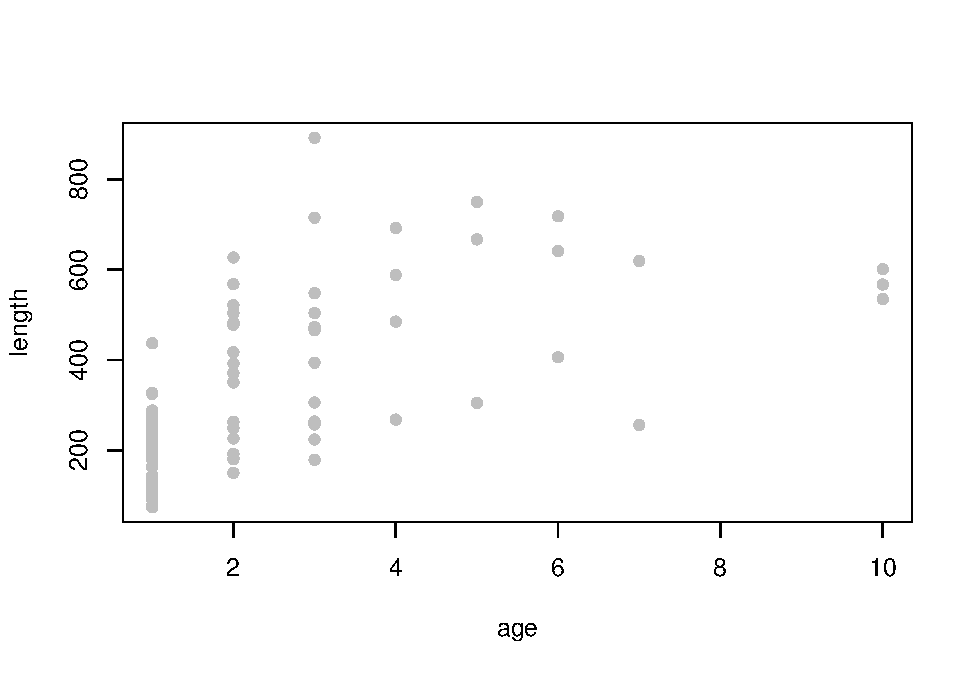
\includegraphics{au-r-workshop_files/figure-latex/unnamed-chunk-185-1} \end{center}

Due to a large amount of variability in individual growth rates, the
relationship looks pretty noisy. Notice how you have mostly young fish
in your sample: this is characteristic of ``random'' sampling of fish
populations.

Suppose you would like to obtain the probability that an average-sized
fish of each age is sexually mature. You know that fish of this species
mature at approximately 450 mm, and you simply need to determine the
fraction of all fish at each age are greater than 450 mm. However, you
don't have any observations for some ages (e.g., age 8), so you cannot
simply calculate this fraction based on your raw data. You need to fit
the von Bertalanffy growth model, then carry the statistical uncertainty
from the fitted model forward to the predicted length-at-age. This would
be difficult to obtain using only the coefficient estimates and their
standard errors, because of the non-linear relationship between the
\(x\) and \(y\) variables.

Enter the \textbf{bootstrap}, which is a Monte Carlo analysis using an
observed data set and a model. The \textbf{pseudocode} for a bootstrap
analysis is:

\begin{enumerate}
\def\labelenumi{\arabic{enumi}.}
\tightlist
\item
  Resample from the originial data (with replacement)
\item
  Fit a model of interest
\item
  Derive some quantity of interest from the fitted model
\item
  Repeat steps 1 - 3 many times
\item
  Summarize the randomized quantities from step 4
\end{enumerate}

In this example, you will apply a bootstrap approach to obtain the
distribution of expected fish lengths at each age, then use these
distributions to quantify the probability that an averaged-sized fish of
each age is mature (i.e., greater than 450 mm).

You will write a function for each of steps 1 - 3 above. The first is to
resample the data:

\begin{Shaded}
\begin{Highlighting}[]
\NormalTok{randomize =}\StringTok{ }\ControlFlowTok{function}\NormalTok{(dat) \{}
  \CommentTok{# number of observed pairs}
\NormalTok{  n =}\StringTok{ }\KeywordTok{nrow}\NormalTok{(dat)}
  \CommentTok{# sample the rows to determine which will be kept}
\NormalTok{  keep =}\StringTok{ }\KeywordTok{sample}\NormalTok{(}\DataTypeTok{x =} \DecValTok{1}\OperatorTok{:}\NormalTok{n, }\DataTypeTok{size =}\NormalTok{ n, }\DataTypeTok{replace =}\NormalTok{ T)}
  \CommentTok{# retreive these rows from the data}
\NormalTok{  dat[keep,]}
\NormalTok{\}}
\end{Highlighting}
\end{Shaded}

Notice the use of \texttt{replace\ =\ T} here: without this, there would
be no bootstrap. You would just sample the same observations over and
over, their order in the rows would just be shuffled. Next, write a
function to fit the model (revisit Section \ref{nls} for more details on
\texttt{nls()}):

\begin{Shaded}
\begin{Highlighting}[]
\NormalTok{fit_vonB =}\StringTok{ }\ControlFlowTok{function}\NormalTok{(dat) \{}
  \KeywordTok{nls}\NormalTok{(length }\OperatorTok{~}\StringTok{ }\NormalTok{linf }\OperatorTok{*}\StringTok{ }\NormalTok{(}\DecValTok{1} \OperatorTok{-}\StringTok{ }\KeywordTok{exp}\NormalTok{(}\OperatorTok{-}\NormalTok{k }\OperatorTok{*}\StringTok{ }\NormalTok{(age }\OperatorTok{-}\StringTok{ }\NormalTok{t0))),}
      \DataTypeTok{data =}\NormalTok{ dat,}
      \DataTypeTok{start =} \KeywordTok{c}\NormalTok{(}\DataTypeTok{linf =} \DecValTok{600}\NormalTok{, }\DataTypeTok{k =} \FloatTok{0.3}\NormalTok{, }\DataTypeTok{t0 =} \OperatorTok{-}\FloatTok{0.2}\NormalTok{)}
\NormalTok{      )}
\NormalTok{\}}
\end{Highlighting}
\end{Shaded}

This function will return a fitted model object when executed. Next,
write a function to predict mean length-at-age:

\begin{Shaded}
\begin{Highlighting}[]
\CommentTok{# create a vector of ages}
\NormalTok{ages =}\StringTok{ }\KeywordTok{min}\NormalTok{(dat}\OperatorTok{$}\NormalTok{age)}\OperatorTok{:}\KeywordTok{max}\NormalTok{(dat}\OperatorTok{$}\NormalTok{age)}
\NormalTok{pred_vonB =}\StringTok{ }\ControlFlowTok{function}\NormalTok{(fit) \{}
  \CommentTok{# extract the coefficients}
\NormalTok{  ests =}\StringTok{ }\KeywordTok{coef}\NormalTok{(fit)}
  \CommentTok{# predict length-at-age}
\NormalTok{  ests[}\StringTok{"linf"}\NormalTok{] }\OperatorTok{*}\StringTok{ }\NormalTok{(}\DecValTok{1} \OperatorTok{-}\StringTok{ }\KeywordTok{exp}\NormalTok{(}\OperatorTok{-}\NormalTok{ests[}\StringTok{"k"}\NormalTok{] }\OperatorTok{*}\StringTok{ }\NormalTok{(ages }\OperatorTok{-}\StringTok{ }\NormalTok{ests[}\StringTok{"t0"}\NormalTok{])))}
\NormalTok{\}}
\end{Highlighting}
\end{Shaded}

Notice your function will use the object \texttt{ages} even though it
was not defined in the function. This has to do with \textbf{lexical
scoping} and \textbf{environments}, which are beyond the scope of this
introductional material\footnote{If you'd like more details, see Hadley
  Wickham's page on it:
  \url{http://adv-r.had.co.nz/Functions.html\#lexical-scoping}}.
Basically, if an object with the same name as one defined in the
function exists outside of the function, the function will use the one
that is defined within the function. If there is no object defined in
the function with that name, it will look outside of the function for
that object.

Now, use these three functions to perform one iteration:

\begin{Shaded}
\begin{Highlighting}[]
\KeywordTok{pred_vonB}\NormalTok{(}\DataTypeTok{fit =} \KeywordTok{fit_vonB}\NormalTok{(}\DataTypeTok{dat =} \KeywordTok{randomize}\NormalTok{(}\DataTypeTok{dat =}\NormalTok{ dat)))}
\end{Highlighting}
\end{Shaded}

You can wrap this inside of a \texttt{replicate()} call to perform step
4 above:

\begin{Shaded}
\begin{Highlighting}[]
\KeywordTok{set.seed}\NormalTok{(}\DecValTok{2}\NormalTok{)}
\NormalTok{out =}\StringTok{ }\KeywordTok{replicate}\NormalTok{(}\DataTypeTok{n =} \DecValTok{100}\NormalTok{, }\DataTypeTok{expr =}\NormalTok{ \{}
  \KeywordTok{pred_vonB}\NormalTok{(}\DataTypeTok{fit =} \KeywordTok{fit_vonB}\NormalTok{(}\DataTypeTok{dat =} \KeywordTok{randomize}\NormalTok{(}\DataTypeTok{dat =}\NormalTok{ dat)))}
\NormalTok{\})}

\KeywordTok{dim}\NormalTok{(out)}
\end{Highlighting}
\end{Shaded}

\begin{verbatim}
## [1]  10 100
\end{verbatim}

It appears the rows are different ages and the columns are different
bootstrapped iterations. Summarize the random lengths at each age:

\begin{Shaded}
\begin{Highlighting}[]
\NormalTok{summ =}\StringTok{ }\KeywordTok{apply}\NormalTok{(out, }\DecValTok{1}\NormalTok{, }\ControlFlowTok{function}\NormalTok{(x) }\KeywordTok{c}\NormalTok{(}\DataTypeTok{mean =} \KeywordTok{mean}\NormalTok{(x), }\KeywordTok{quantile}\NormalTok{(x, }\KeywordTok{c}\NormalTok{(}\FloatTok{0.025}\NormalTok{, }\FloatTok{0.975}\NormalTok{))))}
\end{Highlighting}
\end{Shaded}

Plot the data, the summarized ranges of mean lengths, and the length at
which all fish are assumed to be mature (450 mm)

\begin{Shaded}
\begin{Highlighting}[]
\KeywordTok{plot}\NormalTok{(length }\OperatorTok{~}\StringTok{ }\NormalTok{age, }\DataTypeTok{data =}\NormalTok{ dat, }\DataTypeTok{col =} \StringTok{"grey"}\NormalTok{, }\DataTypeTok{pch =} \DecValTok{16}\NormalTok{,}
     \DataTypeTok{ylim =} \KeywordTok{c}\NormalTok{(}\DecValTok{0}\NormalTok{, }\KeywordTok{max}\NormalTok{(dat}\OperatorTok{$}\NormalTok{length, summ[}\StringTok{"97.5%"}\NormalTok{,])),}
     \DataTypeTok{ylab =} \StringTok{"Length (mm)"}\NormalTok{, }\DataTypeTok{xlab =} \StringTok{"Age (years)"}\NormalTok{)}
\KeywordTok{lines}\NormalTok{(summ[}\StringTok{"mean"}\NormalTok{,] }\OperatorTok{~}\StringTok{ }\NormalTok{ages, }\DataTypeTok{lwd =} \DecValTok{2}\NormalTok{)}
\KeywordTok{lines}\NormalTok{(summ[}\StringTok{"2.5%"}\NormalTok{,] }\OperatorTok{~}\StringTok{ }\NormalTok{ages, }\DataTypeTok{col =} \StringTok{"grey"}\NormalTok{)}
\KeywordTok{lines}\NormalTok{(summ[}\StringTok{"97.5%"}\NormalTok{,] }\OperatorTok{~}\StringTok{ }\NormalTok{ages, }\DataTypeTok{col =} \StringTok{"grey"}\NormalTok{)}
\KeywordTok{abline}\NormalTok{(}\DataTypeTok{h =} \DecValTok{450}\NormalTok{, }\DataTypeTok{col =} \StringTok{"blue"}\NormalTok{)}
\end{Highlighting}
\end{Shaded}

\begin{center}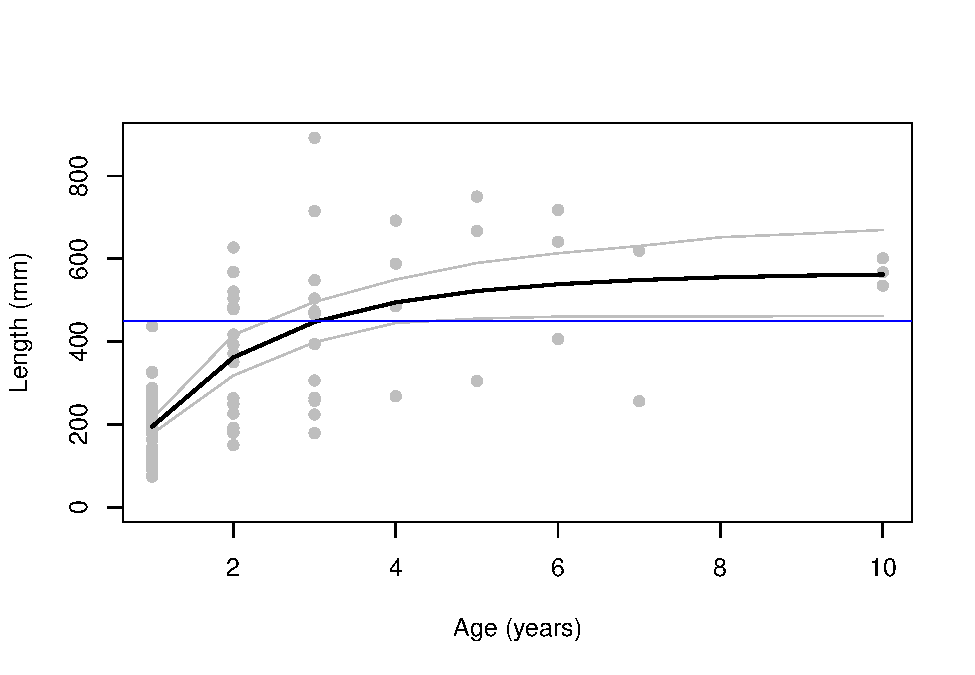
\includegraphics{au-r-workshop_files/figure-latex/unnamed-chunk-192-1} \end{center}

Obtain the fraction of iterations that resulted in the mean
length-at-age being greater than 450 mm. This is interpretted as the
probability that the average-sized fish of each age is mature:

\begin{Shaded}
\begin{Highlighting}[]
\NormalTok{p_mat =}\StringTok{ }\KeywordTok{apply}\NormalTok{(out, }\DecValTok{1}\NormalTok{, }\ControlFlowTok{function}\NormalTok{(x) }\KeywordTok{mean}\NormalTok{(x }\OperatorTok{>}\StringTok{ }\DecValTok{450}\NormalTok{))}
\KeywordTok{plot}\NormalTok{(p_mat }\OperatorTok{~}\StringTok{ }\NormalTok{ages, }\DataTypeTok{type =} \StringTok{"b"}\NormalTok{, }\DataTypeTok{pch =} \DecValTok{17}\NormalTok{,}
     \DataTypeTok{xlab =} \StringTok{"Age (years)"}\NormalTok{, }\DataTypeTok{ylab =} \StringTok{"Probability of Average Fish Mature"}\NormalTok{)}
\end{Highlighting}
\end{Shaded}

\begin{center}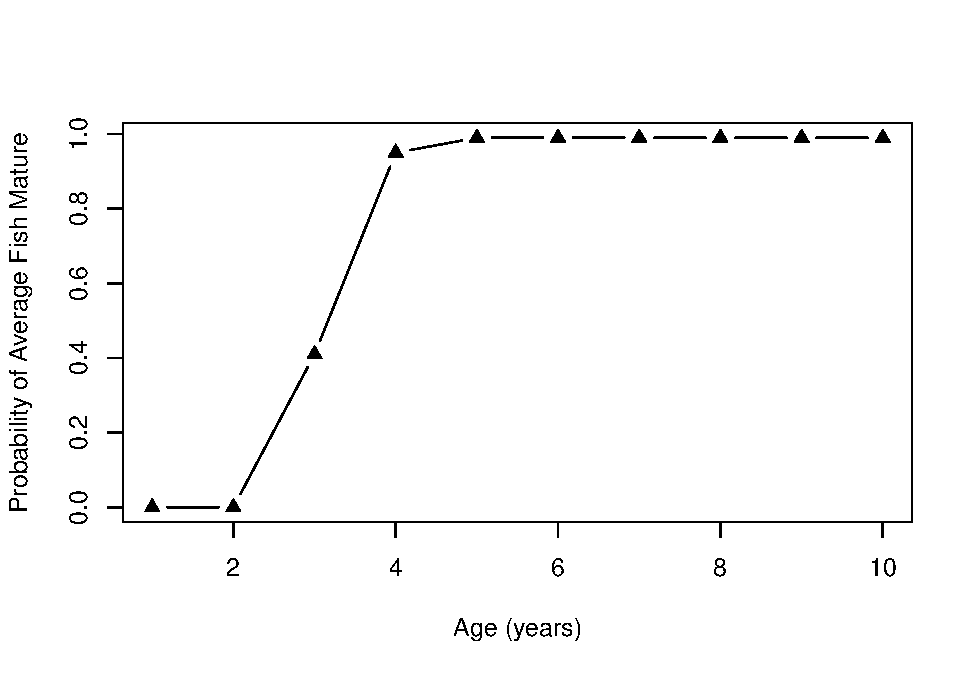
\includegraphics{au-r-workshop_files/figure-latex/unnamed-chunk-193-1} \end{center}

This \textbf{maturity schedule} can be used by fishery managers in
attempting to decide which ages should be allowed to be harvested and
which should be allowed to grow more\footnote{possibly in a
  \textbf{yield-per-recruit} analysis}. Because each age has an
associated expected length, managers can use what they know about the
size selectivity of various gear types to set policies that attempt to
target some ages more than others.

\subsection{Permutation Test}\label{perm-test-ex}

In the previous example (Section \ref{boot-test-ex}), you learned about
the bootstrap. A related Monte Carlo analysis is the \textbf{permutation
test}. This is a non-parametric statistical test to determine if there
is a statistically-significant difference in the mean of some quantity
between two populations. It is used in cases where the assumptions of a
generalized linear model may not be met, but a p-value is still
required.

The \textbf{pseudocode} for the permutation test is:

\begin{enumerate}
\def\labelenumi{\arabic{enumi}.}
\tightlist
\item
  Calculate the difference between means based on the original data set
\item
  Shuffle the group assignments randomly among the observations
\item
  Calculate the difference between the randomly-assigned groups
\item
  Repeat steps 2 - 3 many times. This builds the \textbf{null
  distribution}: the distribution of the test statistic (the difference)
  assuming the null hypothesis that there is not difference in means is
  true
\item
  Determine what fraction of the absolute differences were larger than
  the original difference. This constitutes a \textbf{two-tailed}
  p-value. One-tailed tests can also be derived using the same steps 1 -
  4, which is left as an exercise.
\end{enumerate}

Use the data set \texttt{ponds.csv} for this example (see the
\protect\hyperlink{data-sets}{instructions} on aquiring data files).
This is the same data set used for \protect\hyperlink{ex1b}{Exercise
1B}, revisit that exercise for details on this hypothetical data set.
Read in and plot the data:

\begin{Shaded}
\begin{Highlighting}[]
\NormalTok{dat =}\StringTok{ }\KeywordTok{read.csv}\NormalTok{(}\StringTok{"ponds.csv"}\NormalTok{)}
\KeywordTok{plot}\NormalTok{(chl.a }\OperatorTok{~}\StringTok{ }\NormalTok{treatment, }\DataTypeTok{data =}\NormalTok{ dat)}
\end{Highlighting}
\end{Shaded}

\begin{center}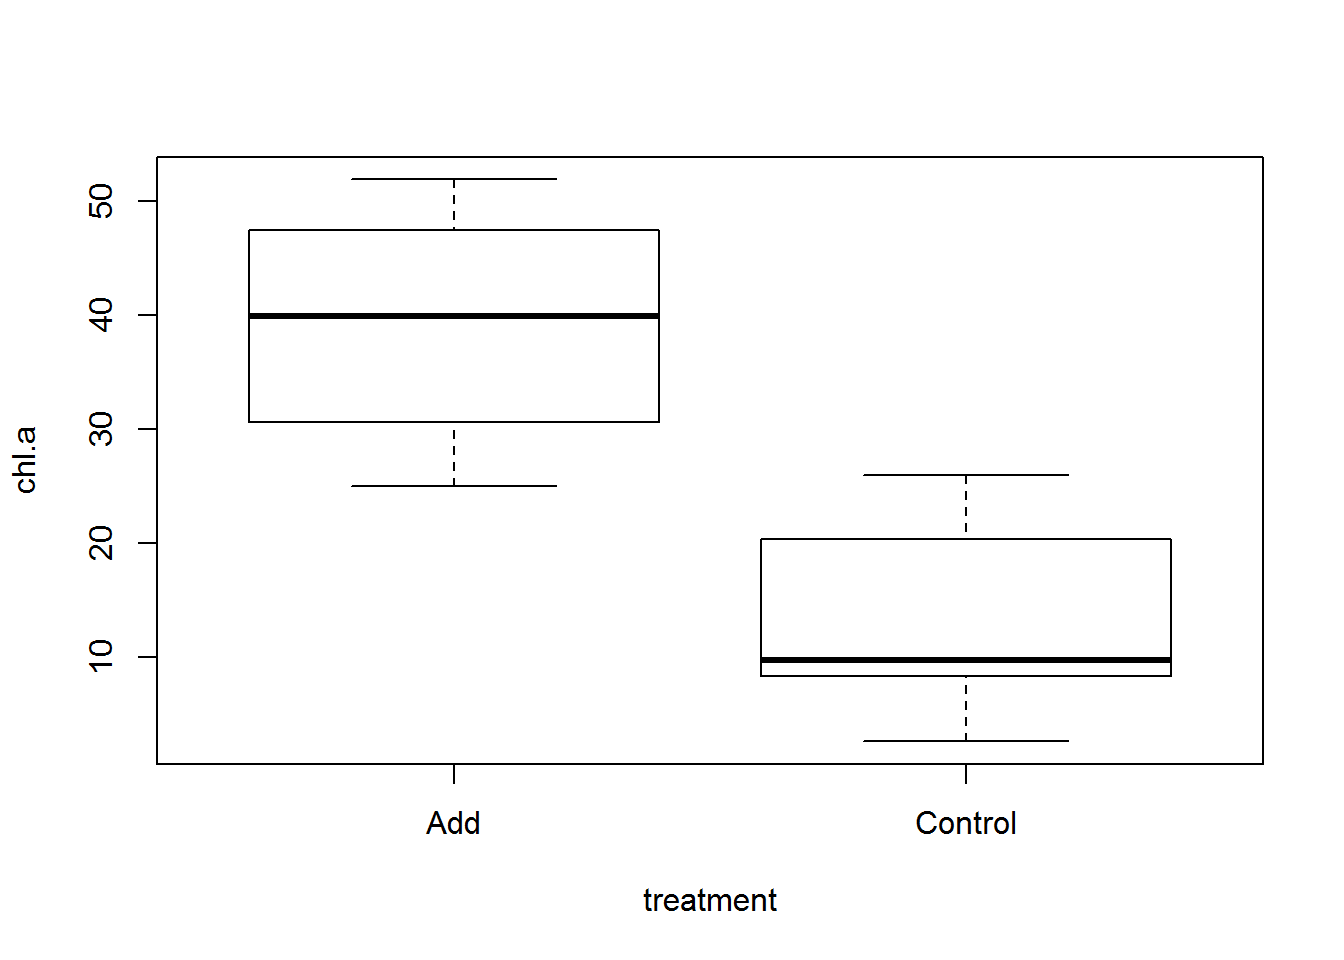
\includegraphics{au-r-workshop_files/figure-latex/unnamed-chunk-195-1} \end{center}

It appears as though there is a relatively strong signal indicating a
difference. Use the permutation test to determine if it is statistically
significant. Step 1 from the pseudocode is to caluclate the observed
difference between groups:

\begin{Shaded}
\begin{Highlighting}[]
\NormalTok{Dobs =}\StringTok{ }\KeywordTok{mean}\NormalTok{(dat}\OperatorTok{$}\NormalTok{chl.a[dat}\OperatorTok{$}\NormalTok{treatment }\OperatorTok{==}\StringTok{ "Add"}\NormalTok{]) }\OperatorTok{-}\StringTok{ }\KeywordTok{mean}\NormalTok{(dat}\OperatorTok{$}\NormalTok{chl.a[dat}\OperatorTok{$}\NormalTok{treatment }\OperatorTok{==}\StringTok{ "Control"}\NormalTok{])}
\NormalTok{Dobs}
\end{Highlighting}
\end{Shaded}

\begin{verbatim}
## [1] 26.166
\end{verbatim}

Write a function to perform one iteration of steps 2 - 3 from the
pseudocode:

\begin{Shaded}
\begin{Highlighting}[]
\CommentTok{# x is the group: Add or Control}
\CommentTok{# y is chl.a}
\NormalTok{perm =}\StringTok{ }\ControlFlowTok{function}\NormalTok{(x, y) \{}
  \CommentTok{# turn x to a character, easier to deal with}
\NormalTok{  x =}\StringTok{ }\KeywordTok{as.character}\NormalTok{(x)}
  \CommentTok{# shuffle the x values:}
\NormalTok{  x_shuff =}\StringTok{ }\KeywordTok{sample}\NormalTok{(x)}
  \CommentTok{# calculate the mean of each group:}
\NormalTok{  x_bar_add =}\StringTok{ }\KeywordTok{mean}\NormalTok{(y[x_shuff }\OperatorTok{==}\StringTok{ "Add"}\NormalTok{])}
\NormalTok{  x_bar_ctl =}\StringTok{ }\KeywordTok{mean}\NormalTok{(y[x_shuff }\OperatorTok{==}\StringTok{ "Control"}\NormalTok{])}
  \CommentTok{# calculate the difference:}
\NormalTok{  x_bar_add }\OperatorTok{-}\StringTok{ }\NormalTok{x_bar_ctl}
\NormalTok{\}}
\end{Highlighting}
\end{Shaded}

Use your function once:

\begin{Shaded}
\begin{Highlighting}[]
\KeywordTok{perm}\NormalTok{(}\DataTypeTok{x =}\NormalTok{ dat}\OperatorTok{$}\NormalTok{treatment, }\DataTypeTok{y =}\NormalTok{ dat}\OperatorTok{$}\NormalTok{chl.a)}
\end{Highlighting}
\end{Shaded}

\begin{verbatim}
## [1] -11.15
\end{verbatim}

Perform step 4 from the pseudocode by replicating your \texttt{perm()}
function many times:

\begin{Shaded}
\begin{Highlighting}[]
\NormalTok{Dnull =}\StringTok{ }\KeywordTok{replicate}\NormalTok{(}\DataTypeTok{n =} \DecValTok{5000}\NormalTok{, }\DataTypeTok{expr =} \KeywordTok{perm}\NormalTok{(}\DataTypeTok{x =}\NormalTok{ dat}\OperatorTok{$}\NormalTok{treatment, }\DataTypeTok{y =}\NormalTok{ dat}\OperatorTok{$}\NormalTok{chl.a))}
\end{Highlighting}
\end{Shaded}

Plot the distribution of the null test statistic and draw a line where
the originally-observed difference falls:

\begin{Shaded}
\begin{Highlighting}[]
\KeywordTok{hist}\NormalTok{(Dnull, }\DataTypeTok{col =} \StringTok{"grey"}\NormalTok{)}
\KeywordTok{abline}\NormalTok{(}\DataTypeTok{v =}\NormalTok{ Dobs, }\DataTypeTok{col =} \StringTok{"blue"}\NormalTok{, }\DataTypeTok{lwd =} \DecValTok{3}\NormalTok{, }\DataTypeTok{lty =} \DecValTok{2}\NormalTok{)}
\end{Highlighting}
\end{Shaded}

\begin{center}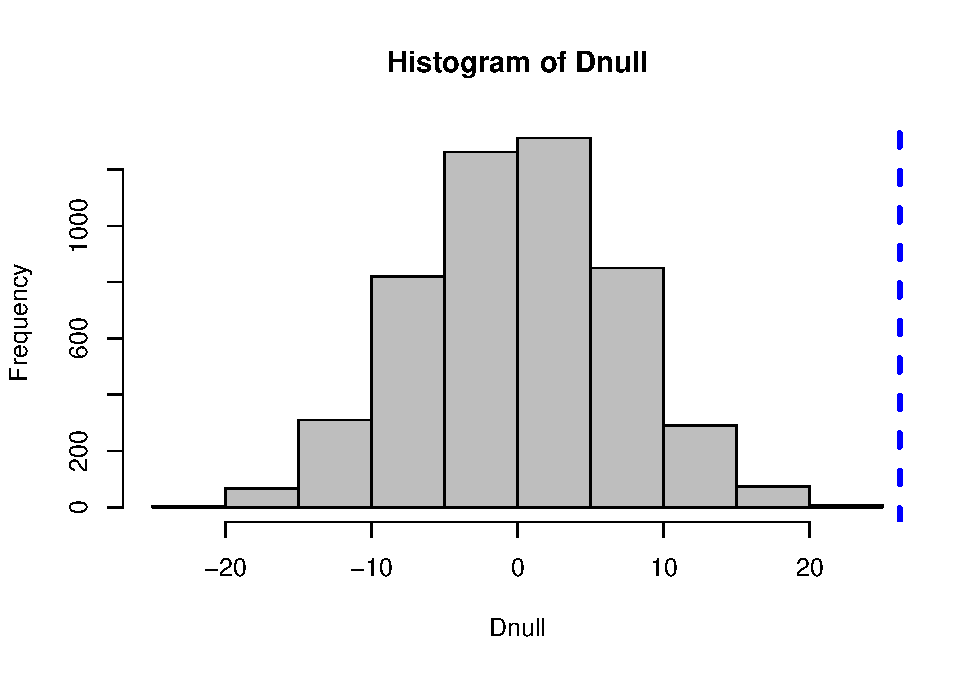
\includegraphics{au-r-workshop_files/figure-latex/unnamed-chunk-200-1} \end{center}

Notice the null distribution is centered on zero: this is because the
null hypothesis is that there is no difference. The observation (blue
line) falls way in the upper tail of the null distribution, indicating
it is unlikely an effect that large was observed by random chance. The
two-tailed p-value can be calculated as:

\begin{Shaded}
\begin{Highlighting}[]
\KeywordTok{mean}\NormalTok{(}\KeywordTok{abs}\NormalTok{(Dnull) }\OperatorTok{>=}\StringTok{ }\NormalTok{Dobs)}
\end{Highlighting}
\end{Shaded}

\begin{verbatim}
## [1] 0
\end{verbatim}

Very few (or zero) of the random data sets resulted in a difference
greater than what was observed, indicating there is statisitcal support
to the hypothesis that there is a non-zero difference between the two
nutrient treatments.

\begin{center}\rule{0.5\linewidth}{\linethickness}\end{center}

\section{Exercise 4}\label{exercise-4}

In these exercises, you will be adapting the code written in this
chapter to investigate slightly different questions. You should create a
new R script \texttt{Ex4.R} in your working directory for these
exercises so your chapter code is left unchanged. Exercise 4A is based
solely on the required material and Exercises 4B - 4F are based on the
example cases. You should work through each example before attempting
each of the later exercises.

\emph{The solutions to this exercise are found at the end of this book
(\protect\hyperlink{ex4a-answers}{here}). You are \textbf{strongly
recommended} to make a good attempt at completing this exercise on your
own and only look at the solutions when you are truly stumped.}

\subsection*{Exercise 4A: Required Material
Only}\label{exercise-4a-required-material-only}
\addcontentsline{toc}{subsection}{Exercise 4A: Required Material Only}

These questions are based on the material in Sections \ref{randomness} -
\ref{mc-summaries} only.

\begin{enumerate}
\def\labelenumi{\arabic{enumi}.}
\tightlist
\item
  Simulate flipping an unfair coin (probability of heads = 0.6) 100
  times using \texttt{rbinom()}. Count the number of heads and tails.
\item
  Simulate flipping the same unfair coin 100 times, but using
  \texttt{sample()} instead. Determine what fraction of the flips
  resulted in heads.
\item
  Simulate rolling a fair 6-sided die 100 times using \texttt{sample()}.
  Determine what fraction of the rolls resulted in an even number.
\item
  Simulate rolling the same die 100 times, but use the function
  \texttt{rmultinom()} instead. Look at the help file for details on how
  to use this function. Determine what fraction of the rolls resulted in
  an odd number.
\end{enumerate}

\protect\hyperlink{ex4a-answers}{Solutions}

\subsection*{\texorpdfstring{Exercise 4B: Test
\texttt{rnorm}}{Exercise 4B: Test rnorm}}\label{exercise-4b-test-rnorm}
\addcontentsline{toc}{subsection}{Exercise 4B: Test \texttt{rnorm}}

These questions will require you to adapt the code written in Section
\ref{rnorm-ex}

\begin{enumerate}
\def\labelenumi{\arabic{enumi}.}
\tightlist
\item
  Adapt this example to investigate another univariate probability
  distribution, like \texttt{-lnorm()}, \texttt{-pois()}, or
  \texttt{-beta()}. See the help files (e.g., \texttt{?rpois}) for
  details on how to use each function.
\end{enumerate}

\protect\hyperlink{ex4b-answers}{Solutions}

\subsection*{Exercise 4C: Stochastic Power
Analysis}\label{exercise-4c-stochastic-power-analysis}
\addcontentsline{toc}{subsection}{Exercise 4C: Stochastic Power
Analysis}

These questions will require you to adapt the code written in Section
\ref{power-ex}

\begin{enumerate}
\def\labelenumi{\arabic{enumi}.}
\tightlist
\item
  What sample size \texttt{n} do you need to have a power of 0.8 of
  detecting a significant difference between the two tagging methods?
\item
  How do the inferences from the power analysis change if you are
  interested in \texttt{p\_new\ =\ 0.4} instead of
  \texttt{p\_new\ =\ 0.25}? Do you need to tag more or fewer fish in
  this case?
\item
  Your analysis takes a bit of time to run so you are interested in
  tracking its progress. Add a progress message to your nested
  \texttt{for()} loop that will print the sample size currently being
  analyzed:
\end{enumerate}

\begin{Shaded}
\begin{Highlighting}[]
\ControlFlowTok{for}\NormalTok{ (n }\ControlFlowTok{in} \DecValTok{1}\OperatorTok{:}\NormalTok{N) \{}
  \KeywordTok{cat}\NormalTok{(}\StringTok{"}\CharTok{\textbackslash{}r}\StringTok{"}\NormalTok{, }\StringTok{"Sample Size = "}\NormalTok{, n_try[n])}
  \ControlFlowTok{for}\NormalTok{ (i }\ControlFlowTok{in} \DecValTok{1}\OperatorTok{:}\NormalTok{I) \{}
\NormalTok{    ...}
\NormalTok{  \}}
\NormalTok{\}}
\end{Highlighting}
\end{Shaded}

\protect\hyperlink{ex4c-answers}{Solutions}

\subsection*{Exercise 4D: Harvest Policy
Analysis}\label{exercise-4d-harvest-policy-analysis}
\addcontentsline{toc}{subsection}{Exercise 4D: Harvest Policy Analysis}

These questions will require you to adapt the code written in Section
\ref{harv-ex}

\begin{enumerate}
\def\labelenumi{\arabic{enumi}.}
\tightlist
\item
  Add an argument to \texttt{ricker\_sim()} that will give the user an
  option to create a plot that shows the time series of recruitment,
  harvest, and escapement all on the same plot. Set the default to be to
  not plot the result, in case you forget to turn it off before
  performing the Monte Carlo analysis.
\item
  Add an \emph{error handler} to \texttt{ricker\_sim()} that will cause
  the function to return an error \texttt{if()} the names of the vector
  passed to the \texttt{param} argument aren't what the function is
  expecting. You can use stop(``Error Message Goes Here'') to have your
  function stop and return an error.
\item
  How do the results of the trade-off analysis differ if the process
  error was larger (a larger value of \(\sigma\))?
\item
  Add implementation error to the harvest policy. That is, if the target
  exploitation rate is \(U\), make the real exploitation rate in year
  \(y\) be: \(U_y \sim Beta(a,b)\), where \(a = 100U\) and
  \(b = 100(1-U)\). You can make there be more implementation error by
  inserting a smaller number other than 100 here. How does this affect
  the trade-off analysis?
\end{enumerate}

\protect\hyperlink{ex4d-answers}{Solutions}

\subsection*{Exercise 4E: The
Bootstrap}\label{exercise-4e-the-bootstrap}
\addcontentsline{toc}{subsection}{Exercise 4E: The Bootstrap}

These questions will require you to adapt the code written in Section
\ref{boot-test-ex}

\begin{enumerate}
\def\labelenumi{\arabic{enumi}.}
\tightlist
\item
  Replicate the bootstrap analysis but adapted for the linear regression
  example in Section \ref{regression}. Stop at the step where you
  summarize the 95\% interval range.
\item
  Compare the 95\% bootstrap confidence intervals to the intervals you
  get by running the \texttt{predict} function on the original data set
  with the argument \texttt{interval\ =\ "confidence"} set.
\end{enumerate}

\protect\hyperlink{ex4e-answers}{Solutions}

\subsection*{Exercise 4F: Permutation
Tests}\label{exercise-4f-permutation-tests}
\addcontentsline{toc}{subsection}{Exercise 4F: Permutation Tests}

These questions will require you to adapt the code written in Section
\ref{perm-test-ex}

\begin{enumerate}
\def\labelenumi{\arabic{enumi}.}
\tightlist
\item
  Adapt the code to perform a permutation test for the difference in
  each of the zooplankton densities between treatments. Don't forget to
  fix the missing value in the \texttt{chao} variable. See
  \protect\hyperlink{ex1b}{Exercise 2} for more details on this.
\item
  Adapt the code to perform a permutation test for another data set used
  in this book where there are observations of both a categorical
  variable and a continuous variable. The data sets
  \texttt{sockeye.csv}, \texttt{growth.csv}, or \texttt{creel.csv}
  should be good starting points.
\item
  Add a calculation of the p-value for a one-tailed test (i.e., that the
  difference in means is greater or less than zero). Steps 1 - 4 are the
  same: all you need is \texttt{Dnull} and \texttt{Dobs}. Don't be
  afraid to Google this if you are confused.
\end{enumerate}

\protect\hyperlink{ex4f-answers}{Solutions}

\chapter{Large Data Manipulation}\label{ch5}

\section*{Chapter Overview}\label{chapter-overview-4}
\addcontentsline{toc}{section}{Chapter Overview}

Any data analyst will tell you that oftentimes the most difficult part
of an analysis is simply getting the data in the proper format. Real
data sets are messy: they have missing values, variables are often
stored in multiple columns that would be better stored as rows, the same
factor level may be coded as two or more different types\footnote{E.g.,
  \texttt{"hatch"}, ``\texttt{Hatch}'', and \texttt{"HATCH"} are all
  treated as different factor levels in R}, or the required data are in
several separate files. You get the point: sometimes significant
data-wrangling may be required before you perform an analysis.

In this chapter, you will learn tricks to do more advanced data
manipulation in R using two R \textbf{packages}:

\begin{itemize}
\tightlist
\item
  \texttt{\{reshape2\}}: used for changing data between formats (wide
  and long)
\item
  \texttt{\{dplyr\}}: used for large data manipulations with a
  consistent and readable format.
\end{itemize}

You will be turning daily observations of harvest and escapement (fish
that are not harvested) into annual totals for the purpose of fitting a
\textbf{spawner-recruit analysis} on a hypothetical pink salmon
(\emph{Oncorhynchus gorbuscha}) data set. More details and context on
these terms and topics will be provided later.

\textbf{IMPORTANT NOTE}: If you did not attend the sessions
corresponding to Chapters \ref{ch1} or \ref{ch2}, you are recommended to
walk through the material found in those chapters before proceeding to
this material. Additionally, you will find the material in Section
\ref{nls} helpful for the end of this chapter. Remember that if you are
confused about a topic, you can use \textbf{CTRL + F} to find previous
cases where that topic has been discussed in this book.

\section*{Before You Begin}\label{before-you-begin-3}
\addcontentsline{toc}{section}{Before You Begin}

You should create a new directory and R script for your work in this
Chapter. Create a new R script called \texttt{Ch5.R} and save it in the
directory \texttt{C:/Users/YOU/Documents/R-Book/Chapter5}. Set your
working directory to that location. Revisit the material in Sections
\ref{scripts} and \ref{working-dir} for more details on these steps.

\section{Aquiring and Loading
Packages}\label{aquiring-and-loading-packages}

An \textbf{R package} is a bunch of code, documentation, and data that
someone has written and bundled into a consistent format that allows
other R users to install and use in their R sessions. R packages make R
incredibly flexible and extensible. If you are trying to do a
specialized analysis that is not included in the base R distribution, it
is likely that someone has already written a package that will allow you
to do it!

You will be using some new packages that you likely don't already have
on your computer, so you will need to install them first:

\begin{Shaded}
\begin{Highlighting}[]
\KeywordTok{install.packages}\NormalTok{(}\StringTok{"dplyr"}\NormalTok{)}
\KeywordTok{install.packages}\NormalTok{(}\StringTok{"reshape2"}\NormalTok{)}
\end{Highlighting}
\end{Shaded}

This requires an internet connection. You will see some text display in
the console telling you the packages are being installed. This only
needs to be done once for each version of R you have. If you install a
new version of R, you will likely need to update your packages (i.e.,
re-install them).

Now that the packages are on your computer, you will need to load them
into the current session:

\begin{Shaded}
\begin{Highlighting}[]
\KeywordTok{library}\NormalTok{(dplyr)}
\KeywordTok{library}\NormalTok{(reshape2)}
\end{Highlighting}
\end{Shaded}

These messages are telling you that there are functions in the
\texttt{\{dplyr\}} package that have the same names as those already
being used in the \texttt{\{stats\}} and \texttt{\{base\}} R packages.
This is fine so long as you don't want to use the original functions. If
you wish to use the \texttt{\{base\}} version of the \texttt{filter()}
function rather than the \texttt{\{dplyr\}} version, use it like this:
\texttt{base::filter()}. Each time you close and reopen R, you will need
to load any packages you want to use using \texttt{library()} again.

\section{The Data}\label{the-data}

You have daily observations of catch and escapement for every other year
between 1917 and 2015. Pink salmon have a simple life history where fish
spawned in one odd year return as adults to spawn in the next odd year.
There is a commercial fishery in this system located at the river mouth
which harvests fish as they enter the river. A counting tower is located
upstream of the fishing grounds that counts the number of fish that
escaped the fishery and will have a chance to spawn (this number is
termed ``escapement''). The ultimate goal is to obtain annual totals of
spawners and total run (catch + escapement) for the purpose of fitting a
spawner recruit analysis. You will perform some other analyses along the
way directed at quantifying patterns in run timing.

Read in the two data sets for this chapter (see the
\protect\hyperlink{data-sets}{instructions} for details on acquiring
data files):

\begin{Shaded}
\begin{Highlighting}[]
\NormalTok{catch =}\StringTok{ }\KeywordTok{read.csv}\NormalTok{(}\StringTok{"../Data/daily_catch.csv"}\NormalTok{)}
\NormalTok{esc =}\StringTok{ }\KeywordTok{read.csv}\NormalTok{(}\StringTok{"../Data/daily_escape.csv"}\NormalTok{)}
\end{Highlighting}
\end{Shaded}

Look at the first 6 rows and columns of the \texttt{catch} data:

\begin{Shaded}
\begin{Highlighting}[]
\NormalTok{catch[}\DecValTok{1}\OperatorTok{:}\DecValTok{6}\NormalTok{,}\DecValTok{1}\OperatorTok{:}\DecValTok{6}\NormalTok{]}
\end{Highlighting}
\end{Shaded}

\begin{verbatim}
##   doy y_1917 y_1919 y_1921 y_1923 y_1925
## 1 160    175    229    245    135   2685
## 2 161    221    501   1379   1504   2361
## 3 162    242    355   1149     13    277
## 4 163     90    197     52   2721    548
## 5 164    134    428    674    747   1209
## 6 165     76    224   1211   1231    772
\end{verbatim}

The column \texttt{doy} is the day of the year that record corresponds
to, and each column represents a different year. Notice the format of
the \texttt{esc} data is the same:

\begin{Shaded}
\begin{Highlighting}[]
\NormalTok{esc[}\DecValTok{1}\OperatorTok{:}\DecValTok{6}\NormalTok{,}\DecValTok{1}\OperatorTok{:}\DecValTok{6}\NormalTok{]}
\end{Highlighting}
\end{Shaded}

\begin{verbatim}
##   doy y_1917 y_1919 y_1921 y_1923 y_1925
## 1 161     90    189    161     73   1700
## 2 162    113    412    907    819   1495
## 3 163    124    292    756      7    176
## 4 164     46    162     34   1481    347
## 5 165     69    351    443    407    766
## 6 166     39    184    796    670    489
\end{verbatim}

But notice the first \texttt{doy} is one day later for \texttt{esc} than
for \texttt{catch}. This is because of the time lag for fish to make it
from the fishery grounds to the counting tower (a one day swim: fish
that were in the fishing grounds on day \texttt{d} passed the counting
tower on day \texttt{d+1} if they were not harvested).

\section{\texorpdfstring{Change format using
\texttt{melt()}}{Change format using melt()}}\label{change-format-using-melt}

These data are in what is called \textbf{wide} format: different levels
of the \texttt{year} variable are stored as columns. A \textbf{long}
format would have three columns: one for \texttt{doy}, \texttt{year},
and \texttt{catch} or \texttt{esc}. Turn the \texttt{catch} data frame
into long format using the \texttt{melt()} function from
\texttt{\{reshape2\}}:

\begin{Shaded}
\begin{Highlighting}[]
\NormalTok{long.catch =}\StringTok{ }\KeywordTok{melt}\NormalTok{(catch, }\DataTypeTok{id.var =} \StringTok{"doy"}\NormalTok{,}
                  \DataTypeTok{variable.name =} \StringTok{"year"}\NormalTok{,}
                  \DataTypeTok{value.name =} \StringTok{"catch"}\NormalTok{)}
\KeywordTok{head}\NormalTok{(long.catch)}
\end{Highlighting}
\end{Shaded}

\begin{verbatim}
##   doy   year catch
## 1 160 y_1917   175
## 2 161 y_1917   221
## 3 162 y_1917   242
## 4 163 y_1917    90
## 5 164 y_1917   134
## 6 165 y_1917    76
\end{verbatim}

The first argument is the data frame to reformat, the second argument
(\texttt{id.var}) is the variable that identifies one observation from
another, here it is the \texttt{doy} that the count occurred on. In this
case, it is actually all we need to run \texttt{melt} properly. The
optional \texttt{variable.name} and \texttt{value.name} arguments
specify the names of the other two columns. These default to
``variable'' and ``value'' if not specified. Do the same thing for
escapement:

\begin{Shaded}
\begin{Highlighting}[]
\NormalTok{long.esc =}\StringTok{ }\KeywordTok{melt}\NormalTok{(esc, }\DataTypeTok{id.var =} \StringTok{"doy"}\NormalTok{,}
                \DataTypeTok{variable.name =} \StringTok{"year"}\NormalTok{,}
                \DataTypeTok{value.name =} \StringTok{"esc"}\NormalTok{)}
\KeywordTok{head}\NormalTok{(long.esc)}
\end{Highlighting}
\end{Shaded}

\begin{verbatim}
##   doy   year esc
## 1 161 y_1917  90
## 2 162 y_1917 113
## 3 163 y_1917 124
## 4 164 y_1917  46
## 5 165 y_1917  69
## 6 166 y_1917  39
\end{verbatim}

Anytime you do a large data manipulation like this, you should compare
the new data set with the original to verify that it worked properly.
Ask if \texttt{all} of the daily catches for a given year in the
original data set match up to the new data set:

\begin{Shaded}
\begin{Highlighting}[]
\KeywordTok{all}\NormalTok{(catch}\OperatorTok{$}\NormalTok{y_}\DecValTok{2015} \OperatorTok{==}\StringTok{ }\NormalTok{long.catch[long.catch}\OperatorTok{$}\NormalTok{year }\OperatorTok{==}\StringTok{ "y_2015"}\NormalTok{, }\StringTok{"catch"}\NormalTok{])}
\end{Highlighting}
\end{Shaded}

\begin{verbatim}
## [1] TRUE
\end{verbatim}

The single \texttt{TRUE} indicates that every element matches up for
2015 in the catch data, just like they should.

To reverse this action (i.e., to go from long format to wide format),
you would use the \texttt{dcast()} function from \texttt{\{reshape2\}}:

\begin{Shaded}
\begin{Highlighting}[]
\KeywordTok{dcast}\NormalTok{(long.catch, doy }\OperatorTok{~}\StringTok{ }\NormalTok{year, }\DataTypeTok{value.var =} \StringTok{"catch"}\NormalTok{)}
\end{Highlighting}
\end{Shaded}

The formula specifies which variables are ID variables on the left-hand
side, and which variable should get expanded to multiple columns. The
\texttt{value.var} argument indicates which variable will be placed into
the columns.

\section{\texorpdfstring{Join Data Sets with
\texttt{merge()}}{Join Data Sets with merge()}}\label{join-data-sets-with-merge}

You now have two long format data sets. You can turn them into one data
set with the \texttt{merge()} function (which is actually in the
\texttt{\{base\}} package). \texttt{merge()} takes two data frames and
joins them based on certain grouping variables. Here, you want to
combine the data frames \texttt{long.catch} and \texttt{long.esc} into
one data frame, and match the rows by the \texttt{doy} and \texttt{year}
for each unique pair:

\begin{Shaded}
\begin{Highlighting}[]
\NormalTok{dat =}\StringTok{ }\KeywordTok{merge}\NormalTok{(}\DataTypeTok{x =}\NormalTok{ long.esc, }\DataTypeTok{y =}\NormalTok{ long.catch,}
            \DataTypeTok{by =} \KeywordTok{c}\NormalTok{(}\StringTok{"doy"}\NormalTok{, }\StringTok{"year"}\NormalTok{), }\DataTypeTok{all =}\NormalTok{ T)}
\KeywordTok{head}\NormalTok{(dat)}
\end{Highlighting}
\end{Shaded}

\begin{verbatim}
##   doy   year esc catch
## 1 160 y_1917  NA   175
## 2 160 y_1919  NA   229
## 3 160 y_1921  NA   245
## 4 160 y_1923  NA   135
## 5 160 y_1925  NA  2685
## 6 160 y_1927  NA   163
\end{verbatim}

The \texttt{all\ =\ T} argument is important to specify here. It says
that you wish to keep \textbf{all} of the unique records in the columns
passed to \texttt{by} from both data frames. The \texttt{doy} in the
catch data ranges from day 160 to day 209, whereas for escapement it
ranges from day 161 to day 210. In this system, the fishery opens on the
160\textsuperscript{th} day of every year, and the counting tower starts
the 161\textsuperscript{st} day. If you didn't use \texttt{all\ =\ T},
you would drop all the rows in each data set that do not have a match
the other data set (you would lose day 160 and day 210 from every year).
Notice that because no escapement observations were ever made one
\texttt{doy} 160, the \texttt{esc} values on this day is \texttt{NA}.

Notice how the data set is now ordered by \texttt{doy} instead of
\texttt{year}. This is not a problem, but if you want to reorder the
data frame by \texttt{year}, you can use the \texttt{arrange()} function
from \texttt{\{dplyr\}}:

\begin{Shaded}
\begin{Highlighting}[]
\KeywordTok{head}\NormalTok{(}\KeywordTok{arrange}\NormalTok{(dat, year))}
\end{Highlighting}
\end{Shaded}

\begin{verbatim}
##   doy   year esc catch
## 1 160 y_1917  NA   175
## 2 161 y_1917  90   221
## 3 162 y_1917 113   242
## 4 163 y_1917 124    90
## 5 164 y_1917  46   134
## 6 165 y_1917  69    76
\end{verbatim}

\section{Lagged vectors}\label{lagged-vectors}

The present task is to the calculate daily cumulative run
proportion\footnote{This is the fraction of all fish that came back each
  year that did so on or before a given day} in 2015 for comparison to
the other years. Given the information you have, this task would be very
cumbersome if not for the flexibility allowed by \texttt{\{dplyr\}}.

Remember the counting tower is an average one day swim for the salmon
from the fishing grounds. This means that the escapement counts are
\textbf{lagged} relative to the catch counts. If you want the daily run
(defined as the number in fishing grounds each day), you need to account
for this lag. An easy way to think about the lag is to show it
graphically. First, pull out one year of data using the
\texttt{filter()} function in \texttt{\{dplyr\}}:

\begin{Shaded}
\begin{Highlighting}[]
\NormalTok{y15 =}\StringTok{ }\KeywordTok{filter}\NormalTok{(dat, year }\OperatorTok{==}\StringTok{ "y_2015"}\NormalTok{)}
\KeywordTok{head}\NormalTok{(y15)}
\end{Highlighting}
\end{Shaded}

\begin{verbatim}
##   doy   year  esc catch
## 1 160 y_2015   NA  3342
## 2 161 y_2015 2293  2352
## 3 162 y_2015 1614    88
## 4 163 y_2015   61  3270
## 5 164 y_2015 2244  5080
## 6 165 y_2015 3486   379
\end{verbatim}

The \texttt{\{base\}} analog to the \texttt{filter()} function is:

\begin{Shaded}
\begin{Highlighting}[]
\NormalTok{y15 =}\StringTok{ }\NormalTok{dat[dat}\OperatorTok{$}\NormalTok{year }\OperatorTok{==}\StringTok{ "y_2015"}\NormalTok{, ]}
\CommentTok{# or}
\NormalTok{y15 =}\StringTok{ }\KeywordTok{subset}\NormalTok{(dat, year }\OperatorTok{==}\StringTok{ "y_2015"}\NormalTok{)}
\end{Highlighting}
\end{Shaded}

They take about the same amount of code to write, but \texttt{filter()}
has some advantages when used with other \texttt{\{dplyr\}} functions
that will be discussed later. Now plot the daily catch and escapement
(not cumulative yet) for 2015:

\begin{Shaded}
\begin{Highlighting}[]
\KeywordTok{plot}\NormalTok{(catch }\OperatorTok{~}\StringTok{ }\NormalTok{doy, }\DataTypeTok{data =}\NormalTok{ y15, }\DataTypeTok{type =} \StringTok{"b"}\NormalTok{, }\DataTypeTok{pch =} \DecValTok{16}\NormalTok{, }\DataTypeTok{col =} \StringTok{"blue"}\NormalTok{,}
     \DataTypeTok{xlab =} \StringTok{"DOY"}\NormalTok{, }\DataTypeTok{ylab =} \StringTok{"Count"}\NormalTok{, }\DataTypeTok{main =} \StringTok{"Raw Data"}\NormalTok{)}
\KeywordTok{lines}\NormalTok{(esc }\OperatorTok{~}\StringTok{ }\NormalTok{doy, }\DataTypeTok{data =}\NormalTok{ y15, }\DataTypeTok{type =} \StringTok{"b"}\NormalTok{, }\DataTypeTok{pch =} \DecValTok{16}\NormalTok{, }\DataTypeTok{col =} \StringTok{"red"}\NormalTok{)}
\KeywordTok{legend}\NormalTok{(}\StringTok{"topright"}\NormalTok{, }\DataTypeTok{legend =} \KeywordTok{c}\NormalTok{(}\StringTok{"Catch"}\NormalTok{, }\StringTok{"Escapement"}\NormalTok{), }
       \DataTypeTok{col =} \KeywordTok{c}\NormalTok{(}\StringTok{"blue"}\NormalTok{, }\StringTok{"red"}\NormalTok{), }\DataTypeTok{pch =} \DecValTok{16}\NormalTok{, }\DataTypeTok{lty =} \DecValTok{1}\NormalTok{, }\DataTypeTok{bty =} \StringTok{"n"}\NormalTok{, }\DataTypeTok{cex =} \FloatTok{0.8}\NormalTok{)}
\end{Highlighting}
\end{Shaded}

\begin{center}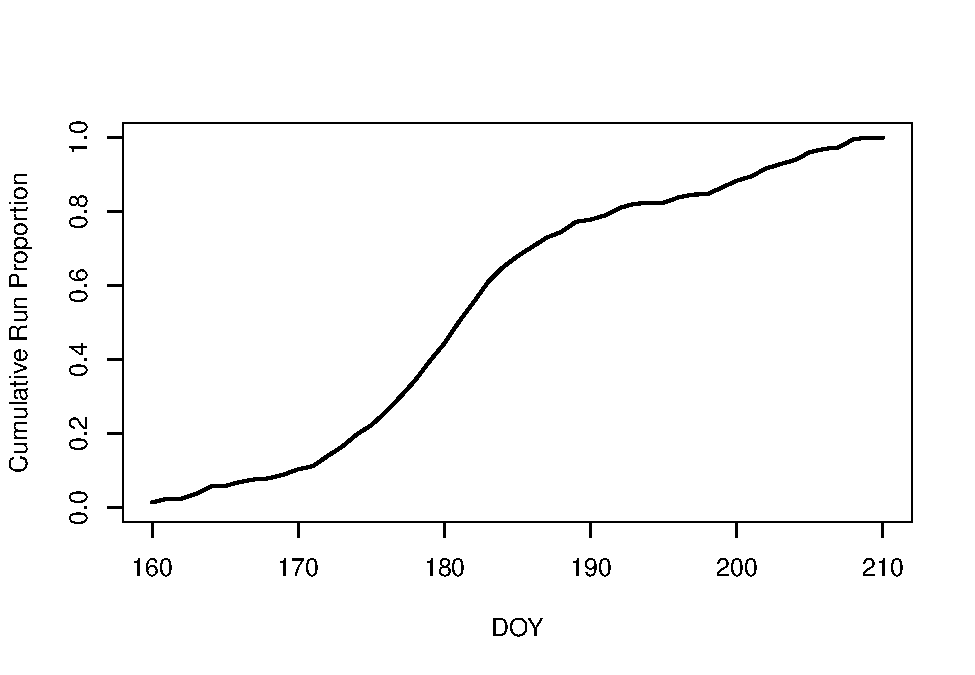
\includegraphics{au-r-workshop_files/figure-latex/unnamed-chunk-219-1} \end{center}

Notice how the escapement counts are shifted to the right by one day.
This is the lag. To account for it, you can use the \texttt{lag()}
function from \texttt{\{dplyr\}}. \texttt{lag()} works by lagging some
vector by \texttt{n} elements (it shifts every element in the vector to
the right by one place by putting \texttt{n} \texttt{NAs} at the front
and removing the last \texttt{n} elements from the original vector). One
way to fix the lag problem would be to use \texttt{lag()} on
\texttt{catch} to make the days match up with \texttt{esc} (don't lag
\texttt{esc} because that would just lag it by \texttt{n} additional
days):

\begin{Shaded}
\begin{Highlighting}[]
\KeywordTok{plot}\NormalTok{(}\KeywordTok{lag}\NormalTok{(catch, }\DataTypeTok{n =} \DecValTok{1}\NormalTok{) }\OperatorTok{~}\StringTok{ }\NormalTok{doy, }\DataTypeTok{data =}\NormalTok{ y15, }\DataTypeTok{type =} \StringTok{"b"}\NormalTok{, }\DataTypeTok{pch =} \DecValTok{16}\NormalTok{, }\DataTypeTok{col =} \StringTok{"blue"}\NormalTok{,}
     \DataTypeTok{xlab =} \StringTok{"DOY"}\NormalTok{, }\DataTypeTok{ylab =} \StringTok{"Count"}\NormalTok{, }\DataTypeTok{main =} \StringTok{"With lag(catch)"}\NormalTok{)}
\KeywordTok{lines}\NormalTok{(esc }\OperatorTok{~}\StringTok{ }\NormalTok{doy, }\DataTypeTok{data =}\NormalTok{ y15, }\DataTypeTok{type =} \StringTok{"b"}\NormalTok{, }\DataTypeTok{pch =} \DecValTok{16}\NormalTok{, }\DataTypeTok{col =} \StringTok{"red"}\NormalTok{)}
\KeywordTok{legend}\NormalTok{(}\StringTok{"topright"}\NormalTok{, }\DataTypeTok{legend =} \KeywordTok{c}\NormalTok{(}\StringTok{"Catch"}\NormalTok{, }\StringTok{"Escapement"}\NormalTok{),}
       \DataTypeTok{col =} \KeywordTok{c}\NormalTok{(}\StringTok{"blue"}\NormalTok{, }\StringTok{"red"}\NormalTok{), }\DataTypeTok{pch =} \DecValTok{16}\NormalTok{, }\DataTypeTok{lty =} \DecValTok{1}\NormalTok{, }\DataTypeTok{bty =} \StringTok{"n"}\NormalTok{, }\DataTypeTok{cex =} \FloatTok{0.8}\NormalTok{)}
\end{Highlighting}
\end{Shaded}

\begin{center}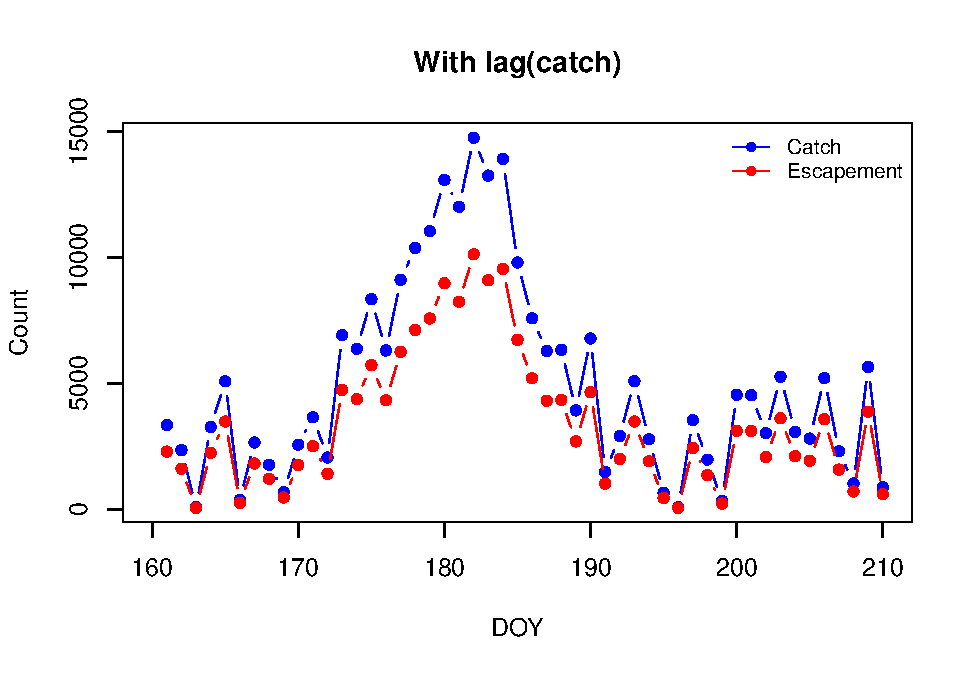
\includegraphics{au-r-workshop_files/figure-latex/unnamed-chunk-220-1} \end{center}

Notice how the two curves line up better now.

\section{\texorpdfstring{Adding columns with
\texttt{mutate()}}{Adding columns with mutate()}}\label{adding-columns-with-mutate}

Apply this same idea to the data set to get the total number of fish
that were in the fishing grounds on each day (the daily run, what was
harvested plus what was not). First, make a function to take two
vectors, lag one, then sum them: this will give you the daily run.
However, you don't need to move catch forward a day, you need to move
escapement back a day. The opposite of \texttt{lag()} is
\texttt{lead()}. The way to think of this is that \texttt{lag()} lags a
vector, and \texttt{lead()} unlags a vector. \texttt{lead()} shifts
every element to the left by \texttt{n} elements by removing the first
\texttt{n} elements of the original vector and adding \texttt{n}
\texttt{NAs} to the end. This is what you want for your function:

\begin{Shaded}
\begin{Highlighting}[]
\NormalTok{lag_sum =}\StringTok{ }\ControlFlowTok{function}\NormalTok{(x, y, }\DataTypeTok{n =} \DecValTok{1}\NormalTok{)\{}
  \CommentTok{# x is lagged from y by n days}
  \KeywordTok{rowSums}\NormalTok{(}\KeywordTok{cbind}\NormalTok{(}\KeywordTok{lead}\NormalTok{(x, n), y), }\DataTypeTok{na.rm =}\NormalTok{ T)}
\NormalTok{\}}
\end{Highlighting}
\end{Shaded}

Note the use of \texttt{na.rm\ =\ T} to specify that summing a number
with an \texttt{NA} should still return a number. If two \texttt{NAs}
are summed, the result will be a zero.

Try out the \texttt{lag\_sum()} function:

\begin{Shaded}
\begin{Highlighting}[]
\KeywordTok{lag_sum}\NormalTok{(y15}\OperatorTok{$}\NormalTok{esc, y15}\OperatorTok{$}\NormalTok{catch)}
\end{Highlighting}
\end{Shaded}

You will want to add this column to your data set. You add columns in
\texttt{\{dplyr\}} using \texttt{mutate()}:

\begin{Shaded}
\begin{Highlighting}[]
\NormalTok{y15 =}\StringTok{ }\KeywordTok{mutate}\NormalTok{(y15, }\DataTypeTok{run =} \KeywordTok{lag_sum}\NormalTok{(esc, catch))}
\end{Highlighting}
\end{Shaded}

The \texttt{\{base\}} equivalent to \texttt{mutate()} is:

\begin{Shaded}
\begin{Highlighting}[]
\NormalTok{y15}\OperatorTok{$}\NormalTok{run =}\StringTok{ }\KeywordTok{lag_sum}\NormalTok{(y15}\OperatorTok{$}\NormalTok{esc, y15}\OperatorTok{$}\NormalTok{catch)}
\end{Highlighting}
\end{Shaded}

\texttt{mutate()} has advantages when used with other \texttt{\{dplyr\}}
functions that will be shown soon. Use the new variable \texttt{run} to
calculate two new variables: the cumulative run by day (\texttt{crun})
and cumulative run proportion by day (\texttt{cprun}). Cumulative means
that each new element is the value that occurred on that day plus all of
the values that happened on days before it. You can use R's
\texttt{cumsum()} for this:

\begin{Shaded}
\begin{Highlighting}[]
\NormalTok{y15 =}\StringTok{ }\KeywordTok{mutate}\NormalTok{(y15, }\DataTypeTok{crun =} \KeywordTok{cumsum}\NormalTok{(run), }\DataTypeTok{cprun =}\NormalTok{ crun}\OperatorTok{/}\KeywordTok{sum}\NormalTok{(run, }\DataTypeTok{na.rm =}\NormalTok{ T))}
\end{Highlighting}
\end{Shaded}

Here is one advantage of \texttt{mutate()}: you can refer to a variable
you just created to make a new variable within the same function. You
would have to split this into two lines to do it in \texttt{\{base\}}.
Indeed, you could have made \texttt{run}, \texttt{crun}, and
\texttt{cprun} all in the same \texttt{mutate()} call. Plot
\texttt{cprun}\footnote{It doesn't look like much, but this information
  is incredibly important for fishery managers. It provides information
  on how much of the annual run has passed on each day. You can see that
  the rate of change is the fastest in the middle of the run, this
  corresponds to the major hump in the plots you made earlier (which
  were raw numbers by day). Of course during the run, the managers don't
  know what proportion of the total run has passed because they don't
  know the total number of fish that will come that season, but by
  characterizing the mean and variability of the different run
  completion proportions on each day in the past, they can have some
  idea of how much of the run to expect yet to come on any given day.}:

\begin{Shaded}
\begin{Highlighting}[]
\KeywordTok{plot}\NormalTok{(cprun }\OperatorTok{~}\StringTok{ }\NormalTok{doy, }\DataTypeTok{data =}\NormalTok{ y15, }\DataTypeTok{type =} \StringTok{"l"}\NormalTok{, }\DataTypeTok{ylim =} \KeywordTok{c}\NormalTok{(}\DecValTok{0}\NormalTok{, }\DecValTok{1}\NormalTok{),}
     \DataTypeTok{xlab =} \StringTok{"DOY"}\NormalTok{, }\DataTypeTok{ylab =} \StringTok{"Cumulative Run Proportion"}\NormalTok{, }\DataTypeTok{lwd =} \DecValTok{2}\NormalTok{)}
\end{Highlighting}
\end{Shaded}

\begin{center}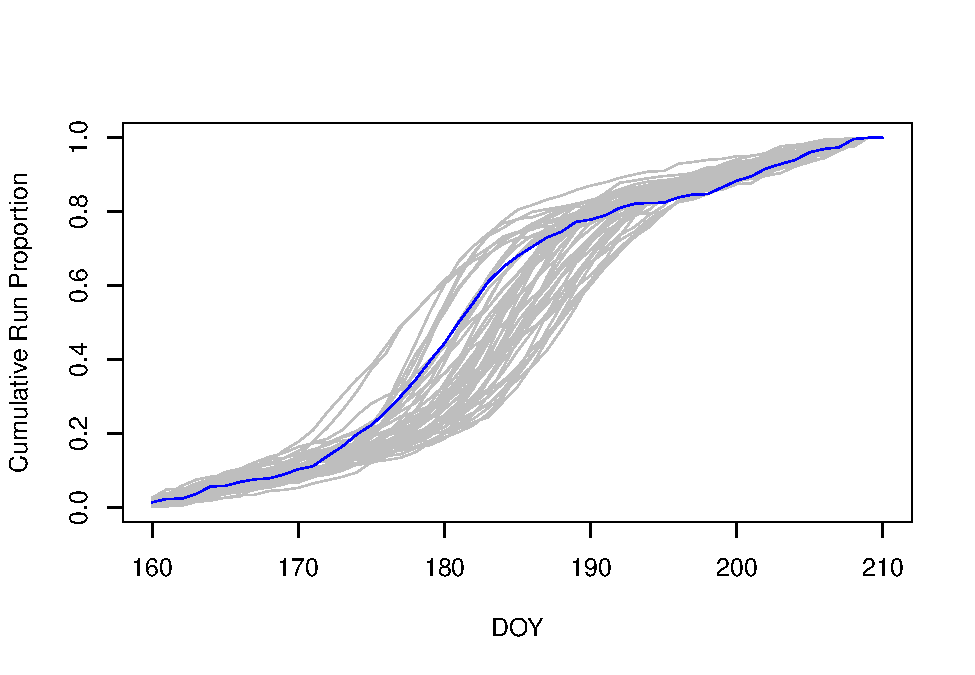
\includegraphics{au-r-workshop_files/figure-latex/unnamed-chunk-226-1} \end{center}

\section{Apply to all years}\label{apply-to-all-years}

You have just obtained the daily and cumulative run for one year (2015),
but \texttt{\{dplyr\}} makes it easy to apply these same manipulations
to all years. To really see the advantage, you'll need to learn to use
piping. A code \textbf{pipe} is one that takes the result of one
function and inserts it into the input of another function. Here is a
basic example of a pipe:

\begin{Shaded}
\begin{Highlighting}[]
\KeywordTok{rnorm}\NormalTok{(}\DecValTok{10}\NormalTok{) }\OperatorTok\StringTok{ }\NormalTok{length}
\end{Highlighting}
\end{Shaded}

\begin{verbatim}
## [1] 10
\end{verbatim}

The pipe took the result of \texttt{rnorm(10)} and passed it as the
first argument to the \texttt{length} function. This allows you to
string together commands so you aren't continuously making intermediate
objects or nesting a ton of functions together. The pipe essentially
does this:

\begin{Shaded}
\begin{Highlighting}[]
\NormalTok{x =}\StringTok{ }\KeywordTok{rnorm}\NormalTok{(}\DecValTok{10}\NormalTok{); }\KeywordTok{length}\NormalTok{(x); }\KeywordTok{rm}\NormalTok{(x)}
\end{Highlighting}
\end{Shaded}

\begin{verbatim}
## [1] 10
\end{verbatim}

The reason piping works so well with \texttt{\{dplyr\}} is because its
functions are designed to take a data frame as input as the first
argument and return another data frame as output, which allows you to
string them together with pipes. Do a more complex pipe: take your main
data frame (\texttt{dat}), group it by \texttt{year}, and pass it to a
\texttt{mutate()} call that will add the new three columns to the entire
data set:

\begin{Shaded}
\begin{Highlighting}[]
\NormalTok{dat =}\StringTok{ }\NormalTok{dat }\OperatorTok
\StringTok{  }\KeywordTok{group_by}\NormalTok{(year) }\OperatorTok
\StringTok{  }\KeywordTok{mutate}\NormalTok{(}\DataTypeTok{run =} \KeywordTok{lag_sum}\NormalTok{(esc, catch), }
         \DataTypeTok{crun =} \KeywordTok{cumsum}\NormalTok{(run), }
         \DataTypeTok{cprun =}\NormalTok{ crun}\OperatorTok{/}\KeywordTok{sum}\NormalTok{(run, }\DataTypeTok{na.rm =}\NormalTok{ T))}

\KeywordTok{arrange}\NormalTok{(dat, year)}
\end{Highlighting}
\end{Shaded}

\begin{verbatim}
## # A tibble: 2,550 x 7
## # Groups:   year [50]
##      doy year     esc catch   run  crun  cprun
##    <int> <fct>  <int> <int> <dbl> <dbl>  <dbl>
##  1   160 y_1917    NA   175  265.  265. 0.0127
##  2   161 y_1917    90   221  334.  599. 0.0288
##  3   162 y_1917   113   242  366.  965. 0.0464
##  4   163 y_1917   124    90  136. 1101. 0.0530
##  5   164 y_1917    46   134  203. 1304. 0.0627
##  6   165 y_1917    69    76  115. 1419. 0.0683
##  7   166 y_1917    39    89  134. 1553. 0.0747
##  8   167 y_1917    45   139  210. 1763. 0.0848
##  9   168 y_1917    71   127  192. 1955. 0.0941
## 10   169 y_1917    65    61   92. 2047. 0.0985
## # ... with 2,540 more rows
\end{verbatim}

The \texttt{group\_by()} function is spectacular: you grouped the data
frame by \texttt{year}, which tells the rest of the functions in the
pipe to apply its commands to each year independently. With this
function, you can group your data in any way you please and calculate
statistics on a group-by-group basis. Note that in this example, it
doesn't do much for you, because the data are so neat (all years have
same number of days, \texttt{NAs} in all of the same places, etc.), but
for data that are messier, this trick is very handy. Also note that the
\texttt{dat} object looks a little different. When you print it, it only
shows the first 10 rows. This is a \texttt{\{dplyr\}} feature that
prevents you from printing a huge data set to the console.

Now plot the cumulative run proportion by day for each year,
highlighting 2015:

\begin{Shaded}
\begin{Highlighting}[]
\CommentTok{# make an empty plot}
\KeywordTok{plot}\NormalTok{(}\DataTypeTok{x =} \DecValTok{0}\NormalTok{, }\DataTypeTok{y =} \DecValTok{0}\NormalTok{, }\DataTypeTok{type =} \StringTok{"n"}\NormalTok{, }\DataTypeTok{xlim =} \KeywordTok{range}\NormalTok{(dat}\OperatorTok{$}\NormalTok{doy), }\DataTypeTok{ylim =} \KeywordTok{c}\NormalTok{(}\DecValTok{0}\NormalTok{,}\DecValTok{1}\NormalTok{),}
     \DataTypeTok{xlab =} \StringTok{"DOY"}\NormalTok{, }\DataTypeTok{ylab =} \StringTok{"Cumulative Run Proportion"}\NormalTok{)}

\NormalTok{years =}\StringTok{ }\KeywordTok{levels}\NormalTok{(dat}\OperatorTok{$}\NormalTok{year)}

\CommentTok{# use sapply to "loop" through years, drawing lines for each}
\NormalTok{tmp =}\StringTok{ }\KeywordTok{sapply}\NormalTok{(years, }\ControlFlowTok{function}\NormalTok{(x) \{}
  \KeywordTok{lines}\NormalTok{(cprun }\OperatorTok{~}\StringTok{ }\NormalTok{doy, }\DataTypeTok{data =} \KeywordTok{filter}\NormalTok{(dat, year }\OperatorTok{==}\StringTok{ }\NormalTok{x),}
        \DataTypeTok{col =} \KeywordTok{ifelse}\NormalTok{(x }\OperatorTok{==}\StringTok{ "y_2015"}\NormalTok{, }\StringTok{"blue"}\NormalTok{, }\StringTok{"grey"}\NormalTok{))}
\NormalTok{\})}
\end{Highlighting}
\end{Shaded}

\begin{center}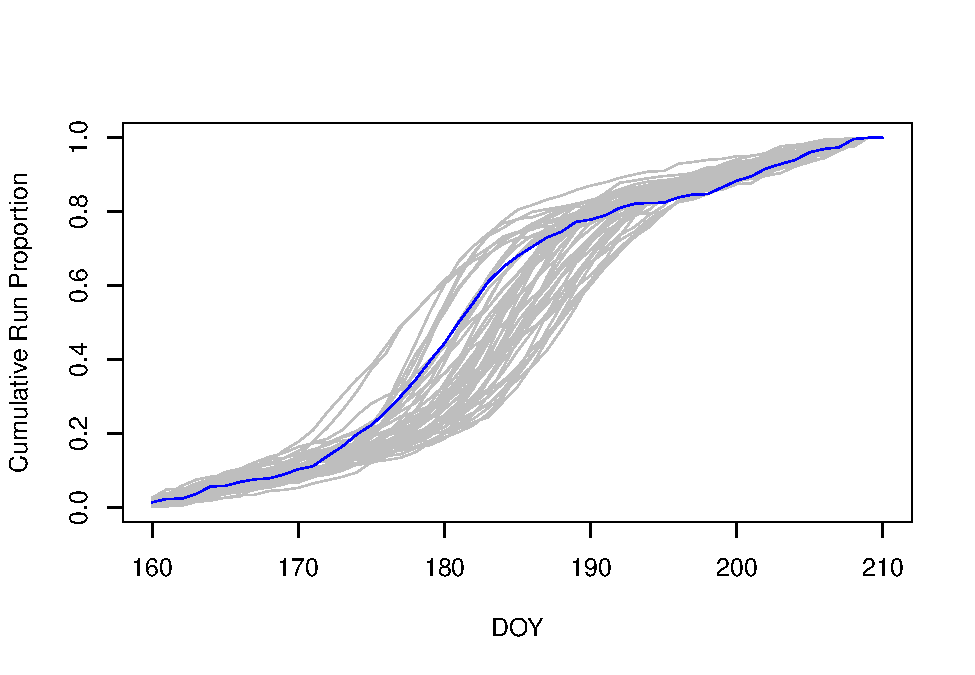
\includegraphics{au-r-workshop_files/figure-latex/unnamed-chunk-230-1} \end{center}

\section{\texorpdfstring{Calculate Daily Means with
\texttt{summarize()}}{Calculate Daily Means with summarize()}}\label{calculate-daily-means-with-summarize}

Oftentimes, you want to calculate a statistic for a value across
grouping variables, like year or site or day. Remember the
\texttt{tapply()} function does this in \texttt{\{base\}}. Here you want
to calculate the mean cumulative run proportion for each day averaged
across years. For this, you can make use of the \texttt{summarize()}
function in \texttt{\{dplyr\}}. Begin by ungrouping the data to remove
the \texttt{year} groups and grouping the data by \texttt{doy}. This
will allow you to calculate the mean proportion by day. You then pass
this grouped data frame to \texttt{summarize()} which will apply the
\texttt{mean()} function to the cumulative run proportions across all
years on a particular day. It will do this for all days:

\begin{Shaded}
\begin{Highlighting}[]
\NormalTok{mean_cprun =}\StringTok{ }\NormalTok{dat }\OperatorTok\StringTok{ }
\StringTok{  }\NormalTok{ungroup }\OperatorTok\StringTok{ }
\StringTok{  }\KeywordTok{group_by}\NormalTok{(doy) }\OperatorTok
\StringTok{  }\KeywordTok{summarize}\NormalTok{(}\DataTypeTok{cprun =} \KeywordTok{mean}\NormalTok{(cprun))}
\KeywordTok{head}\NormalTok{(mean_cprun)}
\end{Highlighting}
\end{Shaded}

\begin{verbatim}
## # A tibble: 6 x 2
##     doy   cprun
##   <int>   <dbl>
## 1   160 0.00970
## 2   161 0.0194 
## 3   162 0.0291 
## 4   163 0.0387 
## 5   164 0.0491 
## 6   165 0.0579
\end{verbatim}

The way to do this in \texttt{\{base\}} is with \texttt{tapply()}:

\begin{Shaded}
\begin{Highlighting}[]
\KeywordTok{tapply}\NormalTok{(dat}\OperatorTok{$}\NormalTok{cprun, dat}\OperatorTok{$}\NormalTok{doy, mean)[}\DecValTok{1}\OperatorTok{:}\DecValTok{6}\NormalTok{]}
\end{Highlighting}
\end{Shaded}

\begin{verbatim}
##         160         161         162         163         164         165 
## 0.009699779 0.019400196 0.029111609 0.038735562 0.049130566 0.057901058
\end{verbatim}

Note that you get the same result, only the output from
\texttt{tapply()} is a vector, and the output of \texttt{summarize()} is
a data frame.

One disadvantage of the \texttt{summarize()} function, however, is that
it can only be used to apply functions that give one number as output
(e.g., \texttt{mean()}, \texttt{max()}, \texttt{sd()},
\texttt{length()}, etc.). These are called \textbf{aggregate} functions:
they take a bunch of numbers and aggregate them into one number.
\texttt{tapply()} does not have this constraint. Illustrate this by
trying to use the \texttt{range()} function (which combines the minimum
and maximum values of some vector into another vector of length 2).

\begin{Shaded}
\begin{Highlighting}[]
\CommentTok{# with summarise}
\NormalTok{dat }\OperatorTok\StringTok{ }
\StringTok{  }\NormalTok{ungroup }\OperatorTok
\StringTok{  }\KeywordTok{group_by}\NormalTok{(doy) }\OperatorTok\StringTok{ }
\StringTok{  }\KeywordTok{summarize}\NormalTok{(}\DataTypeTok{range =} \KeywordTok{range}\NormalTok{(cprun))}
\end{Highlighting}
\end{Shaded}

\begin{verbatim}
## Error in summarise_impl(.data, dots): Column `range` must be length 1 (a summary value), not 2
\end{verbatim}

\begin{Shaded}
\begin{Highlighting}[]
\CommentTok{# with tapply}
\KeywordTok{tapply}\NormalTok{(dat}\OperatorTok{$}\NormalTok{cprun, dat}\OperatorTok{$}\NormalTok{doy, range)[}\DecValTok{1}\OperatorTok{:}\DecValTok{5}\NormalTok{]}
\end{Highlighting}
\end{Shaded}

\begin{verbatim}
## $`160`
## [1] 0.0002721184 0.0256423751
## 
## $`161`
## [1] 0.001485884 0.048191292
## 
## $`162`
## [1] 0.003895501 0.057528072
## 
## $`163`
## [1] 0.01450474 0.07435435
## 
## $`164`
## [1] 0.01797648 0.08253284
\end{verbatim}

You can see that \texttt{tapply()} allows you to do this (but gives a
list), whereas \texttt{summarize()} returns a short and informative
error. However, you could very easily fix the problem by making minimum
and maximum columns in the same \texttt{summarize()} call:

\begin{Shaded}
\begin{Highlighting}[]
\NormalTok{dat }\OperatorTok
\StringTok{  }\NormalTok{ungroup }\OperatorTok
\StringTok{  }\KeywordTok{group_by}\NormalTok{(jday) }\OperatorTok
\StringTok{  }\KeywordTok{summarize}\NormalTok{(}\DataTypeTok{min =} \KeywordTok{min}\NormalTok{(cprun), }\DataTypeTok{max =} \KeywordTok{max}\NormalTok{(cprun))}
\end{Highlighting}
\end{Shaded}

Add the mean cumulative run proportion to our plot (use \texttt{lines()}
just like before, add it after the \texttt{sapply()} call):

\begin{Shaded}
\begin{Highlighting}[]
\KeywordTok{lines}\NormalTok{(cprun }\OperatorTok{~}\StringTok{ }\NormalTok{doy, }\DataTypeTok{data =}\NormalTok{ mean_cprun, }\DataTypeTok{lwd =} \DecValTok{3}\NormalTok{)}
\end{Highlighting}
\end{Shaded}

\begin{center}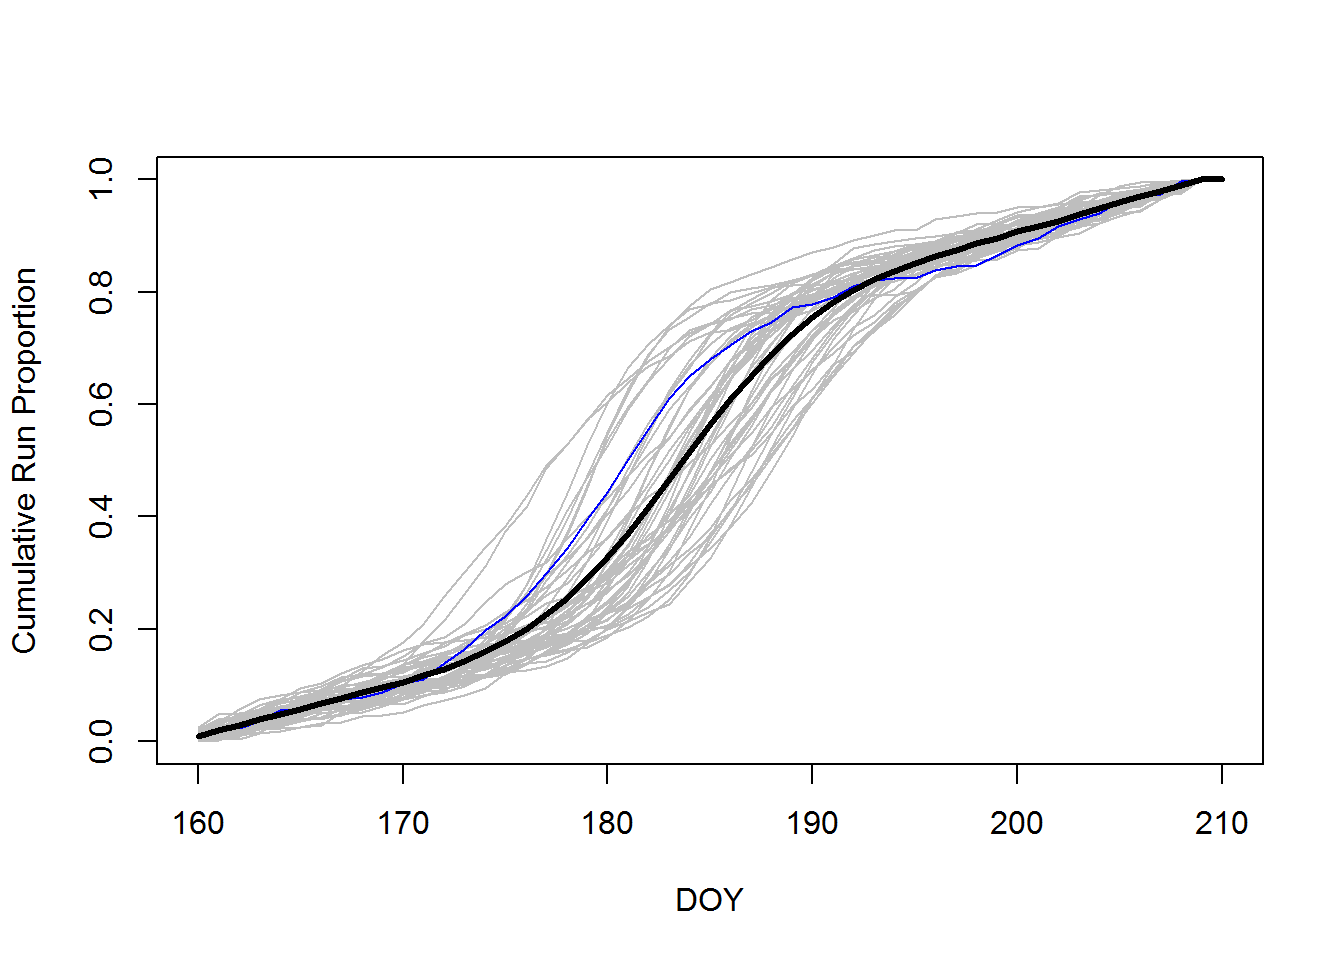
\includegraphics{au-r-workshop_files/figure-latex/unnamed-chunk-236-1} \end{center}

It looks like 2015 started like an average year but the peak of the run
happened a couple days earlier than average.

\section{\texorpdfstring{More
\texttt{summarize()}}{More summarize()}}\label{more-summarize}

Your colleagues have been talking lately about how the run has been
getting earlier and earlier in recent years. To determine if their
claims are correct, you decide to develop a method to find the day on
which 50\% of the run has passed (the median run date) and plot it over
time. If there is a downward trend, then the run has been getting
earlier. First, you need to define another function to find the day that
corresponds to 50\% of the run. If there were days where the cumulative
run on that day equaled exactly 0.5, we could simply use
\texttt{which()}:

\begin{Shaded}
\begin{Highlighting}[]
\NormalTok{ind =}\StringTok{ }\KeywordTok{which}\NormalTok{(dat}\OperatorTok{$}\NormalTok{cprun }\OperatorTok{==}\StringTok{ }\FloatTok{0.5}\NormalTok{)}
\NormalTok{dat}\OperatorTok{$}\NormalTok{jday[ind]}
\end{Highlighting}
\end{Shaded}

The \texttt{which()} function is useful: it returns the indices (element
places) \emph{for which} the condition is \texttt{TRUE} However you need
to do a workaround here, since the median day is likely not exactly 0.5
(and it has to be for \texttt{==} to return a \texttt{TRUE}). We will
give the function two vectors and it will look for a value that is
closest to 0.5 in one vector and pull out the corresponding value in the
second vector:

\begin{Shaded}
\begin{Highlighting}[]
\NormalTok{find_median_doy =}\StringTok{ }\ControlFlowTok{function}\NormalTok{(p,doy) \{}
\NormalTok{  ind =}\StringTok{ }\KeywordTok{which.min}\NormalTok{(}\KeywordTok{abs}\NormalTok{(p }\OperatorTok{-}\StringTok{ }\FloatTok{0.5}\NormalTok{))}
\NormalTok{  doy[ind]}
\NormalTok{\}}
\end{Highlighting}
\end{Shaded}

This function will take every element of \texttt{p}, subtract 0.5, take
the absolute value of the results (make it positive, even if it is
negative), and find the element number that is smallest. This will be
the element with the value closest to 0.5. Note that you could find the
first quartile (0.25) or third quartile (0.75) of the run by inserting
these in for 0.5 above\footnote{This is the perfect kind of thing to
  make an argument to your function!}. Try your function on the 2015
data only:

\begin{Shaded}
\begin{Highlighting}[]
\CommentTok{# use function}
\NormalTok{med_doy15 =}\StringTok{ }\KeywordTok{find_median_doy}\NormalTok{(}\DataTypeTok{p =}\NormalTok{ y15}\OperatorTok{$}\NormalTok{cprun, }\DataTypeTok{doy =}\NormalTok{ y15}\OperatorTok{$}\NormalTok{doy)}

\CommentTok{# pull out the day it called the median to verify it works}
\KeywordTok{filter}\NormalTok{(y15, doy }\OperatorTok{==}\StringTok{ }\NormalTok{med_doy15) }\OperatorTok\StringTok{ }\KeywordTok{select}\NormalTok{(cprun)}
\end{Highlighting}
\end{Shaded}

\begin{verbatim}
##       cprun
## 1 0.5023032
\end{verbatim}

The \texttt{select()} function in \texttt{\{dplyr\}} extracts the
variables requested from the data frame. If there is a grouping variable
set using \texttt{group\_by()}, it will be returned as well. It looks
like the function works. Now combine it with \texttt{summarize()} to
calculate the median day for every year:

\begin{Shaded}
\begin{Highlighting}[]
\NormalTok{med_doy =}\StringTok{ }
\StringTok{  }\NormalTok{dat }\OperatorTok\StringTok{ }
\StringTok{  }\KeywordTok{group_by}\NormalTok{(year) }\OperatorTok\StringTok{ }
\StringTok{  }\KeywordTok{summarize}\NormalTok{(}\DataTypeTok{doy =} \KeywordTok{find_median_doy}\NormalTok{(cprun, doy))}
\KeywordTok{head}\NormalTok{(med_doy)}
\end{Highlighting}
\end{Shaded}

\begin{verbatim}
## # A tibble: 6 x 2
##   year     doy
##   <fct>  <int>
## 1 y_1917   184
## 2 y_1919   188
## 3 y_1921   179
## 4 y_1923   184
## 5 y_1925   182
## 6 y_1927   188
\end{verbatim}

Now, use your \texttt{\{dplyr\}} skills to turn the year column into a
numeric variable:

\begin{Shaded}
\begin{Highlighting}[]
\CommentTok{# get years as a number}
\NormalTok{med_doy}\OperatorTok{$}\NormalTok{year =}\StringTok{ }
\StringTok{  }\KeywordTok{ungroup}\NormalTok{(med_doy) }\OperatorTok
\StringTok{  }\CommentTok{# extract only the year column}
\StringTok{  }\KeywordTok{select}\NormalTok{(year) }\OperatorTok
\StringTok{  }\CommentTok{# turn it to a vector and extract unique values}
\StringTok{  }\NormalTok{unlist }\OperatorTok\StringTok{ }\NormalTok{unname }\OperatorTok\StringTok{ }\NormalTok{unique }\OperatorTok
\StringTok{  }\CommentTok{# replace "y_" with nothing}
\StringTok{  }\KeywordTok{gsub}\NormalTok{(}\DataTypeTok{pattern =} \StringTok{"y_"}\NormalTok{, }\DataTypeTok{replacement =} \StringTok{""}\NormalTok{) }\OperatorTok
\StringTok{  }\CommentTok{# turn to a integer vector}
\StringTok{  }\NormalTok{as.integer}

\KeywordTok{plot}\NormalTok{(doy }\OperatorTok{~}\StringTok{ }\NormalTok{year, }\DataTypeTok{data =}\NormalTok{ med_doy, }\DataTypeTok{pch =} \DecValTok{16}\NormalTok{)}
\end{Highlighting}
\end{Shaded}

\begin{center}\includegraphics{au-r-workshop_files/figure-latex/unnamed-chunk-241-1} \end{center}

It doesn't appear that there is a trend in either direction, but fit a
regression line because you can (Section \ref{regression}):

\begin{Shaded}
\begin{Highlighting}[]
\NormalTok{fit =}\StringTok{ }\KeywordTok{lm}\NormalTok{(doy }\OperatorTok{~}\StringTok{ }\NormalTok{year, }\DataTypeTok{data =}\NormalTok{ med_doy)}
\KeywordTok{summary}\NormalTok{(fit)}\OperatorTok{$}\NormalTok{coef}
\end{Highlighting}
\end{Shaded}

\begin{verbatim}
##                  Estimate  Std. Error    t value     Pr(>|t|)
## (Intercept) 193.781416567 27.80436398  6.9694605 8.190067e-09
## year         -0.005138055  0.01414108 -0.3633424 7.179445e-01
\end{verbatim}

\begin{Shaded}
\begin{Highlighting}[]
\KeywordTok{plot}\NormalTok{(doy }\OperatorTok{~}\StringTok{ }\NormalTok{year, }\DataTypeTok{data =}\NormalTok{ med_doy, }\DataTypeTok{pch =} \DecValTok{16}\NormalTok{)}
\KeywordTok{abline}\NormalTok{(fit, }\DataTypeTok{lty =} \DecValTok{2}\NormalTok{)}
\end{Highlighting}
\end{Shaded}

\begin{center}\includegraphics{au-r-workshop_files/figure-latex/unnamed-chunk-242-1} \end{center}

The results tell you that there is a 0.005 day decrease in median run
date for every 1 year that has gone by and that it is not significantly
different from a zero day decrease per year.

\section{Fit the Model}\label{fit-the-model}

You have done some neat data exploration exercises (and hopefully
learned \texttt{\{dplyr\}} and piping along the way!), but you ultimate
task with this data set is to run a spawner-recruit analysis on all the
data. A \textbf{spawner-recruit analysis} is one that links the number
of total fish produced (the recruits) by a given number of spawners (the
escapement). This is done in an attempt to describe the productivity and
carrying capacity of the population and to obtain \textbf{biological
reference points} off of which harvest policies can be set. You will
need to summarize the daily data into annual totals of escapement and
total run:

\begin{Shaded}
\begin{Highlighting}[]
\NormalTok{sr_dat =}\StringTok{ }
\StringTok{  }\NormalTok{dat }\OperatorTok
\StringTok{  }\KeywordTok{summarize}\NormalTok{(}\DataTypeTok{S =} \KeywordTok{sum}\NormalTok{(esc, }\DataTypeTok{na.rm =}\NormalTok{ T),}
            \DataTypeTok{R =} \KeywordTok{sum}\NormalTok{(run, }\DataTypeTok{na.rm =}\NormalTok{ T))}

\KeywordTok{head}\NormalTok{(sr_dat)}
\end{Highlighting}
\end{Shaded}

\begin{verbatim}
## # A tibble: 6 x 3
##   year       S       R
##   <fct>  <int>   <dbl>
## 1 y_1917  7031  20785.
## 2 y_1919 19647  43553.
## 3 y_1921 45106 113682.
## 4 y_1923 69160 196212.
## 5 y_1925 66306 171006.
## 6 y_1927 96622 243212.
\end{verbatim}

You didn't need to use \texttt{group\_by()} here because the data were
still grouped from an earlier task. There is no harm in putting it in,
and it would help make your code more readable if you were to include
it.

That is the main data manipulation you need to do in order to run the
spawner-recruit analysis. You can fit the model using \texttt{nls()}
(Section \ref{nls}). The model you will fit is called a \textbf{Ricker
spawner-recruit model} and has the form:

\begin{equation}
  R_t = \alpha S_{t-1} e^{-\beta S_{t-1} + \varepsilon_t} ,\varepsilon_t \sim N(0,\sigma)
\label{eq:ricker-ch5}
\end{equation}

where \(\alpha\) is a parameter representing the maximum recruits per
spawner (obtained at very low spawner abundances) and \(\beta\) is a
measure of the strength of \textbf{density-dependent mortality}. Notice
that the error term is in the exponent, which makes
\(e^{\varepsilon_t}\) lognormal. To get \texttt{nls()} to fit this
properly, we will need to fit to \(log(R_t)\) as the response variable.
Write a function that will predict log recruitment from spawners given
the two parameters (ignore the error term):

\begin{Shaded}
\begin{Highlighting}[]
\NormalTok{ricker =}\StringTok{ }\ControlFlowTok{function}\NormalTok{(S, alpha, beta) \{}
  \KeywordTok{log}\NormalTok{(alpha }\OperatorTok{*}\StringTok{ }\NormalTok{S }\OperatorTok{*}\StringTok{ }\KeywordTok{exp}\NormalTok{(}\OperatorTok{-}\NormalTok{beta }\OperatorTok{*}\StringTok{ }\NormalTok{S))}
\NormalTok{\}}
\end{Highlighting}
\end{Shaded}

Fit the model to the data using \texttt{nls()}. Before you fit it,
however, you'll need to do another lag. This is because the run that
comes back in one year was spawned by the escapement the previous odd
year (you only have odd years in the data). This time extract the
appropriate years ``by-hand'' rather than using the \texttt{lag()} or
\texttt{lead()} functions as before:

\begin{Shaded}
\begin{Highlighting}[]
\CommentTok{# the number of years}
\NormalTok{nyrs =}\StringTok{ }\KeywordTok{nrow}\NormalTok{(sr_dat)}
\CommentTok{# the spawners to fit to:}
\NormalTok{S_fit =}\StringTok{ }\NormalTok{sr_dat}\OperatorTok{$}\NormalTok{S[}\DecValTok{1}\OperatorTok{:}\NormalTok{(nyrs }\OperatorTok{-}\StringTok{ }\DecValTok{1}\NormalTok{)]}
\CommentTok{# the recruits to fit to:}
\NormalTok{R_fit =}\StringTok{ }\NormalTok{sr_dat}\OperatorTok{$}\NormalTok{R[}\DecValTok{2}\OperatorTok{:}\NormalTok{nyrs]}
\end{Highlighting}
\end{Shaded}

Fit the model:

\begin{Shaded}
\begin{Highlighting}[]
\NormalTok{fit =}\StringTok{ }\KeywordTok{nls}\NormalTok{(}\KeywordTok{log}\NormalTok{(R_fit) }\OperatorTok{~}\StringTok{ }\KeywordTok{ricker}\NormalTok{(S_fit, alpha, beta),}
          \DataTypeTok{start =} \KeywordTok{c}\NormalTok{(}\DataTypeTok{alpha =} \DecValTok{6}\NormalTok{, }\DataTypeTok{beta =} \DecValTok{0}\NormalTok{))}
\KeywordTok{coef}\NormalTok{(fit); }\KeywordTok{summary}\NormalTok{(fit)}\OperatorTok{$}\NormalTok{sigma}
\end{Highlighting}
\end{Shaded}

\begin{verbatim}
##        alpha         beta 
## 5.341553e+00 6.896867e-06
\end{verbatim}

\begin{verbatim}
## [1] 0.4047541
\end{verbatim}

Given that the true values for these data were: \(\alpha = 6\),
\(\beta = 8\times10^{-6}\), and \(\sigma = 0.4\), these estimates look
pretty good.

Plot the recruits versus spawners and the fitted line:

\begin{Shaded}
\begin{Highlighting}[]
\CommentTok{# plot the S-R pairs}
\KeywordTok{plot}\NormalTok{(R_fit }\OperatorTok{~}\StringTok{ }\NormalTok{S_fit, }\DataTypeTok{pch =} \DecValTok{16}\NormalTok{, }\DataTypeTok{col =} \StringTok{"grey"}\NormalTok{, }\DataTypeTok{cex =} \FloatTok{1.5}\NormalTok{,}
     \DataTypeTok{xlim =} \KeywordTok{c}\NormalTok{(}\DecValTok{0}\NormalTok{, }\KeywordTok{max}\NormalTok{(S_fit)), }\DataTypeTok{ylim =} \KeywordTok{c}\NormalTok{(}\DecValTok{0}\NormalTok{, }\KeywordTok{max}\NormalTok{(R_fit)))}
\CommentTok{# extract the estimates}
\NormalTok{ests =}\StringTok{ }\KeywordTok{coef}\NormalTok{(fit)}
\CommentTok{# obtain and draw on a fitted line}
\NormalTok{S_line =}\StringTok{ }\KeywordTok{seq}\NormalTok{(}\DecValTok{0}\NormalTok{, }\KeywordTok{max}\NormalTok{(S_fit), }\DataTypeTok{length =} \DecValTok{100}\NormalTok{)}
\NormalTok{R_line =}\StringTok{ }\KeywordTok{exp}\NormalTok{(}\KeywordTok{ricker}\NormalTok{(}\DataTypeTok{S =}\NormalTok{ S_line,}
                \DataTypeTok{alpha =}\NormalTok{ ests[}\StringTok{"alpha"}\NormalTok{],}
                \DataTypeTok{beta =}\NormalTok{ ests[}\StringTok{"beta"}\NormalTok{]))}
\KeywordTok{lines}\NormalTok{(R_line }\OperatorTok{~}\StringTok{ }\NormalTok{S_line, }\DataTypeTok{lwd =}\DecValTok{3}\NormalTok{)}
\CommentTok{# draw the 1:1 line}
\KeywordTok{abline}\NormalTok{(}\DecValTok{0}\NormalTok{, }\DecValTok{1}\NormalTok{, }\DataTypeTok{lty =} \DecValTok{2}\NormalTok{)}
\end{Highlighting}
\end{Shaded}

\begin{center}\includegraphics{au-r-workshop_files/figure-latex/unnamed-chunk-247-1} \end{center}

The diagonal line is the \textbf{1:1 replacement line}: where 1 spawner
would produce 1 recruit. The distance between this line and the curve is
the theoretical \textbf{harvestable surplus} available at each spawner
abundance that would keep the stock at a fixed abundance. The biological
reference points that might be used in harvest management are:

\begin{eqnarray*}
&& S_{MAX}=\frac{1}{\beta},\\
&& S_{eq}=log(\alpha) S_{MAX},\\
&& S_{MSY}=S_{eq} \left(0.5-0.07*log(\alpha)\right)
\label{eq:ricker-brps}
\end{eqnarray*}

Where \(S_{MAX}\) is the spawner abundance expected to produce the
maximum recruits, \(S_{eq}\) is the spawner abundance that should
produce exactly replacement recruits, and \(S_{MSY}\) is the spawner
abundance that is expected to produce the maximum surplus (all under the
assumption of no environmental variability). You can calculate the
reference points given in Equation \eqref{eq:ricker-brps} from your
parameter estimates:

\begin{Shaded}
\begin{Highlighting}[]
\NormalTok{Smax =}\StringTok{ }\DecValTok{1}\OperatorTok{/}\NormalTok{ests[}\StringTok{"beta"}\NormalTok{]}
\NormalTok{Seq =}\StringTok{ }\KeywordTok{log}\NormalTok{(ests[}\StringTok{"alpha"}\NormalTok{]) }\OperatorTok{*}\StringTok{ }\NormalTok{Smax}
\NormalTok{Smsy =}\StringTok{ }\NormalTok{Seq }\OperatorTok{*}\StringTok{ }\NormalTok{(}\FloatTok{0.5} \OperatorTok{-}\StringTok{ }\FloatTok{0.07} \OperatorTok{*}\StringTok{ }\KeywordTok{log}\NormalTok{(ests[}\StringTok{"alpha"}\NormalTok{]))}
\NormalTok{brps =}\StringTok{ }\KeywordTok{round}\NormalTok{(}\KeywordTok{c}\NormalTok{(}\DataTypeTok{Smax =} \KeywordTok{unname}\NormalTok{(Smax),}
               \DataTypeTok{Seq =} \KeywordTok{unname}\NormalTok{(Seq),}
               \DataTypeTok{Smsy =} \KeywordTok{unname}\NormalTok{(Smsy)), }\OperatorTok{-}\DecValTok{3}\NormalTok{)}
\end{Highlighting}
\end{Shaded}

Draw these reference points onto your plot and label them:

\begin{Shaded}
\begin{Highlighting}[]
\KeywordTok{abline}\NormalTok{(}\DataTypeTok{v =}\NormalTok{ brps, }\DataTypeTok{col =} \StringTok{"blue"}\NormalTok{)}
\KeywordTok{text}\NormalTok{(}\DataTypeTok{x =}\NormalTok{ brps, }\DataTypeTok{y =} \KeywordTok{max}\NormalTok{(R_fit) }\OperatorTok{*}\StringTok{ }\FloatTok{1.08}\NormalTok{, }
     \DataTypeTok{labels =} \KeywordTok{names}\NormalTok{(brps), }\DataTypeTok{xpd =}\NormalTok{ T, }\DataTypeTok{col =} \StringTok{"blue"}\NormalTok{)}
\end{Highlighting}
\end{Shaded}

\begin{center}\includegraphics{au-r-workshop_files/figure-latex/unnamed-chunk-250-1} \end{center}

\begin{center}\rule{0.5\linewidth}{\linethickness}\end{center}

\section*{Exercise 5}\label{exercise-5}
\addcontentsline{toc}{section}{Exercise 5}

In this exercise, you will be working with another simulated salmon data
set (from an age-structured population this time, like Chinook salmon
\emph{Oncorhynchus tshawytscha}). You have information on individual
fish passing a \textbf{weir}. A weir is a blockade in a stream that
biologists use to count fish as they pass by. Most of the day, the weir
is closed and fish stack up waiting to pass. Then a couple times a day,
biologists open a gate in the weir and count fish as they pass. Each
year, the biologists sample a subset of fish that pass by to get age,
sex, and length. There are concerns that by using large mesh gill nets,
the fishery is selectively taking the larger fish and that this is
causing a shift in the size-at-age, age composition, and sex
composition. If this is the case, it could potentially mean a reduction
in productivity since smaller fish have fewer eggs. You are tasked with
analyzing these data to determine if these quantities have changed
overtime. Note that documenting directional changes in these quantities
over time and the co-occurrence of the use of large mesh gill nets does
not imply causation.

\emph{The solutions to this exercise are found at the end of this book
(\protect\hyperlink{ex5-answers}{here}). You are \textbf{strongly
recommended} to make a good attempt at completing this exercise on your
own and only look at the solutions when you are truly stumped.}

Use the data found in \texttt{asl.csv} (\textbf{a}ge, \textbf{s}ex,
\textbf{l}ength) (see the \protect\hyperlink{data-sets}{instructions}
for details on acquiring the data files for this book). Create a new R
script \texttt{Ex5.R} in your working directory. Open this script and
read the data file into R. If this is a new session, load the
\texttt{\{dplyr\}} package.

\begin{enumerate}
\def\labelenumi{\arabic{enumi}.}
\tightlist
\item
  Count the number of females that were sampled each year using the
  \texttt{\{dplyr\}} function \texttt{n()} within a \texttt{summarize()}
  call (\emph{Hint: \texttt{n()} works just like length - it counts the
  number of records}).
\item
  Calculate the proportion of females by year.
\item
  Plot percent females over time. Does it look like the sex composition
  has changed over time?
\item
  Calculate mean length by age, sex, and year.
\item
  Come up with a way to plot a time series of mean length-at-age for
  both sexes. Does it look like mean length-at-age has changed over time
  for either sex?
\end{enumerate}

\begin{center}\rule{0.5\linewidth}{\linethickness}\end{center}

\subsection*{Exercise 5 Bonus}\label{exercise-5-bonus}
\addcontentsline{toc}{subsection}{Exercise 5 Bonus}

\begin{enumerate}
\def\labelenumi{\arabic{enumi}.}
\tightlist
\item
  Calculate the age composition by sex and year (what proportion of all
  the males in a year were age 4, age 5, age 6, age 7, and same for
  females).
\item
  Plot the time series of age composition by sex and year. Does it look
  like age composition has changed over time?
\end{enumerate}

\chapter{Mapping and Spatial Analysis}\label{ch6}

Henry's chapter will go here.

\chapter*{Exercise Solutions}\label{exercise-solutions}
\addcontentsline{toc}{chapter}{Exercise Solutions}

\hypertarget{ex1a-answers}{\section*{Exercise 1A
Solutions}\label{ex1a-answers}}
\addcontentsline{toc}{section}{Exercise 1A Solutions}

\textbf{1. Create a new file in your working directory called
\texttt{Ex1A.R}.}

Go to \emph{File \textgreater{} New File \textgreater{} R Script}. This
will create an untitled R script. Go the \emph{File \textgreater{}
Save}, give it the appropriate name and click \emph{Save}. If your
working directory is already set to
\texttt{C:/Users/YOU/Documents/R-Book/Chapter1}, then the file will be
saved there by default.

You can create a new script using \textbf{CTRL + SHIFT + N} as well.

\textbf{2. Enter these data (found in Table \ref{tab:ex-1-table-pdf})
into vectors. Call the vectors whatever you would like. Should you enter
the data as vectors by rows, or by columns? (Hint: remember the
properties of vectors).}

Because you have both numeric and character data classes for a single
row, you should enter them by columns:

\begin{Shaded}
\begin{Highlighting}[]
\NormalTok{Lake =}\StringTok{ }\KeywordTok{c}\NormalTok{(}\StringTok{"Big"}\NormalTok{, }\StringTok{"Small"}\NormalTok{, }\StringTok{"Square"}\NormalTok{, }\StringTok{"Circle"}\NormalTok{)}
\NormalTok{Area =}\StringTok{ }\KeywordTok{c}\NormalTok{(}\DecValTok{100}\NormalTok{, }\DecValTok{25}\NormalTok{, }\DecValTok{45}\NormalTok{, }\DecValTok{30}\NormalTok{)}
\NormalTok{Time =}\StringTok{ }\KeywordTok{c}\NormalTok{(}\DecValTok{1000}\NormalTok{, }\DecValTok{1200}\NormalTok{, }\DecValTok{1400}\NormalTok{, }\DecValTok{1600}\NormalTok{)}
\NormalTok{Fish =}\StringTok{ }\KeywordTok{c}\NormalTok{(}\DecValTok{643}\NormalTok{, }\DecValTok{203}\NormalTok{, }\DecValTok{109}\NormalTok{, }\DecValTok{15}\NormalTok{)}
\end{Highlighting}
\end{Shaded}

\textbf{3. Combine your vectors into a data frame. Why should you use a
data frame instead of a matrix?}

You should use a data frame because, unlike matrices, they can store
multiple data classes in the different columns. Refer back the sections
on matrices (Section \ref{matrices}) and data frames (Section
\ref{data-frames}) for more details.

\begin{Shaded}
\begin{Highlighting}[]
\NormalTok{df =}\StringTok{ }\KeywordTok{data.frame}\NormalTok{(Lake, Area, Time, Fish)}
\end{Highlighting}
\end{Shaded}

\textbf{4. Subset all of the data from Small Lake.}

Refer back to Section \ref{sub} for details on subsetting using indices
and by column names, see Section \ref{logsub} for details on logical
subsetting.

\begin{Shaded}
\begin{Highlighting}[]
\NormalTok{df[df}\OperatorTok{$}\NormalTok{Lake }\OperatorTok{==}\StringTok{ "Small"}\NormalTok{,]}
\CommentTok{# or}
\NormalTok{df[}\DecValTok{3}\NormalTok{,]}
\end{Highlighting}
\end{Shaded}

\textbf{5. Subset the area for all of the lakes.}

Refer to the suggestions for question 4 for more details.

\begin{Shaded}
\begin{Highlighting}[]
\NormalTok{df}\OperatorTok{$}\NormalTok{Area}
\CommentTok{# or}
\NormalTok{df[,}\DecValTok{2}\NormalTok{]}
\end{Highlighting}
\end{Shaded}

\textbf{6. Subset the number of fish for Big and Square Lakes only.}

Refer to the suggestions for question 4 for more details.

\begin{Shaded}
\begin{Highlighting}[]
\NormalTok{df[df}\OperatorTok{$}\NormalTok{Lake }\OperatorTok{==}\StringTok{ "Big"} \OperatorTok{|}\StringTok{ }\NormalTok{df}\OperatorTok{$}\NormalTok{Lake }\OperatorTok{==}\StringTok{ "Square"}\NormalTok{,}\StringTok{"Fish"}\NormalTok{]}
\CommentTok{# or}
\NormalTok{df}\OperatorTok{$}\NormalTok{Fish[}\KeywordTok{c}\NormalTok{(}\DecValTok{1}\NormalTok{,}\DecValTok{3}\NormalTok{)]}
\end{Highlighting}
\end{Shaded}

\textbf{7. You realize that you sampled 209 fish at Square Lake, not
109. Fix the mistake. There are two ways to do this, can you think of
them both? Which do you think is better?}

The two methods are:

\begin{itemize}
\tightlist
\item
  Fix the mistake in the first place it appears: when you made the
  \texttt{Fish} vector. If you change it there, all other instances in
  your code where you use the \texttt{Fish} object will be fixed after
  you re-run everything.
\end{itemize}

\begin{Shaded}
\begin{Highlighting}[]
\NormalTok{Fish =}\StringTok{ }\KeywordTok{c}\NormalTok{(}\DecValTok{643}\NormalTok{, }\DecValTok{203}\NormalTok{, }\DecValTok{209}\NormalTok{, }\DecValTok{15}\NormalTok{)}
\CommentTok{# re-run the rest of your code and see the error was fixed}
\end{Highlighting}
\end{Shaded}

\begin{itemize}
\tightlist
\item
  Fix the cell in the data frame only:
\end{itemize}

\begin{Shaded}
\begin{Highlighting}[]
\NormalTok{df[df}\OperatorTok{$}\NormalTok{Lake }\OperatorTok{==}\StringTok{ "Square"}\NormalTok{,}\StringTok{"Fish"}\NormalTok{] =}\StringTok{ }\DecValTok{209}
\end{Highlighting}
\end{Shaded}

The second method would only fix the data frame, so if you wanted to use
the vector \texttt{Fish} outside of the data frame, the error would
still be present. For this reason, the first method is likely better.

\textbf{8. Save your script. Close RStudio and re-open your script to
see that it was saved}.

\emph{File \textgreater{} Save} or \textbf{CTRL + S}

\hypertarget{ex1b-answers}{\section*{Exercise 1B
Solutions}\label{ex1b-answers}}
\addcontentsline{toc}{section}{Exercise 1B Solutions}

First, did you find the error? It is the \texttt{\#VALUE!} entry in the
\texttt{chao} column. You should have R treat this as an \texttt{NA}.
The two easiest ways to do this are to either enter \texttt{NA} in that
cell or delete its contents. You can do this easily by opening
\texttt{ponds.csv} in Microsoft Excel or some other spreadsheet editor.

\textbf{1. Read in the data to R and assign it to an object.}

After placing \texttt{ponds.csv} (and all of the other data files) in
the location \texttt{C:/Users/YOU/Documents/R-Book/Data} and creating
\texttt{Ex1B.R} in your working directory:

\begin{Shaded}
\begin{Highlighting}[]
\NormalTok{dat =}\StringTok{ }\KeywordTok{read.csv}\NormalTok{(}\StringTok{"../Data/ponds.csv"}\NormalTok{)}
\end{Highlighting}
\end{Shaded}

\textbf{2. Calculate some basic summary statistics of your data using
the \texttt{summary()} function.}

\begin{Shaded}
\begin{Highlighting}[]
\KeywordTok{summary}\NormalTok{(dat)}
\end{Highlighting}
\end{Shaded}

\textbf{3. Calculate the mean chlorophyll \emph{a} for each pond
(\emph{Hint: pond is a grouping variable}).}

Remember the \texttt{tapply()} function. The first argument is the
variable you wish to calculate a statistic for (chlorophyll), the second
argument is the grouping variable (pond), and the third argument is the
function you wish to apply.

\begin{Shaded}
\begin{Highlighting}[]
\KeywordTok{tapply}\NormalTok{(dat}\OperatorTok{$}\NormalTok{chl.a, dat}\OperatorTok{$}\NormalTok{pond, mean)}
\end{Highlighting}
\end{Shaded}

\textbf{4. Calculate the mean number of \emph{Chaoborus} for each
treatment in each pond using \texttt{tapply()}. (\emph{Hint: You can
group by two variables with:}
\texttt{tapply(dat\$var,\ list(dat\$grp1,\ dat\$grp2),\ fun)}.}

The hint pretty much gives this one away:

\begin{Shaded}
\begin{Highlighting}[]
\KeywordTok{tapply}\NormalTok{(dat}\OperatorTok{$}\NormalTok{chao, }\KeywordTok{list}\NormalTok{(dat}\OperatorTok{$}\NormalTok{pond, dat}\OperatorTok{$}\NormalTok{treatment), mean)}
\end{Highlighting}
\end{Shaded}

\textbf{5. Use the more general \texttt{apply()} function to calculate
the variance for each zooplankton taxa found only in pond S-28.}

First, subset only the correct pond and the zooplankton counts. Then,
specify you want the \texttt{var()} function applied to the second
dimension (columns). Finally, because \texttt{chao} has an \texttt{NA},
you'll need to include the \texttt{na.rm\ =\ T} argument.

\begin{Shaded}
\begin{Highlighting}[]
\KeywordTok{apply}\NormalTok{(dat[dat}\OperatorTok{$}\NormalTok{pond }\OperatorTok{==}\StringTok{ "S.28"}\NormalTok{,}\KeywordTok{c}\NormalTok{(}\StringTok{"daph"}\NormalTok{, }\StringTok{"bosm"}\NormalTok{, }\StringTok{"cope"}\NormalTok{, }\StringTok{"chao"}\NormalTok{)], }\DecValTok{2}\NormalTok{, var, }\DataTypeTok{na.rm =}\NormalTok{ T)}
\end{Highlighting}
\end{Shaded}

\textbf{6. Create a new variable called \texttt{prod} in the data frame
that represents the quantity of chlorophyll \emph{a} in each replicate.
If the chlorophyll \emph{a} in the replicate is greater than 30 give it
a ``high'', otherwise give it a ``low''. (\emph{Hint: are you asking R
to respond to one question or multiple questions? How should this change
the strategy you use?})}

Remember, you can add a new column to a data set using the
\texttt{df\$new\_column\ =\ something()}. If the column
\texttt{new\_column} doesn't exist, it will be added. If it exists
already, it will be written over. You can use \texttt{ifelse()} (not
\texttt{if()}!) to ask if each chlorophyll measurement was greater or
less than 30, and to do something differently based on the result:

\begin{Shaded}
\begin{Highlighting}[]
\NormalTok{dat}\OperatorTok{$}\NormalTok{prod =}\StringTok{ }\KeywordTok{ifelse}\NormalTok{(dat}\OperatorTok{$}\NormalTok{chl.a }\OperatorTok{>}\StringTok{ }\DecValTok{30}\NormalTok{, }\StringTok{"high"}\NormalTok{, }\StringTok{"low"}\NormalTok{)}
\end{Highlighting}
\end{Shaded}

\textbf{Bonus 1. Use \texttt{?table} to figure out how you can use
\texttt{table()} to count how many observations of high and low there
were in each treatment (\emph{Hint: \texttt{table()} will have only two
arguments.}).}

After looking through the help file, you should have seen that
\texttt{table()} has a \texttt{...} as its first argument. After reading
about what it takes there, you would see it is expecting:

\begin{quote}
one or more objects which can be interpretted as factors (including
character strings)\ldots{}
\end{quote}

So if you ran:

\begin{Shaded}
\begin{Highlighting}[]
\KeywordTok{table}\NormalTok{(dat}\OperatorTok{$}\NormalTok{prod, dat}\OperatorTok{$}\NormalTok{treatment)}
\end{Highlighting}
\end{Shaded}

\begin{verbatim}
##       
##        Add Control
##   high   8       0
##   low    2      10
\end{verbatim}

You would get a table showing how many high and low chlorophyll
observations were made for each treatment.

\textbf{Bonus 2. Create a new function called \texttt{product()} that
multiplies any two numbers you specify.}

See Section \ref{user-funcs} for more details on user-defined functions.
Your function might look like this:

\begin{Shaded}
\begin{Highlighting}[]
\NormalTok{product =}\StringTok{ }\ControlFlowTok{function}\NormalTok{(a,b) \{}
\NormalTok{  a }\OperatorTok{*}\StringTok{ }\NormalTok{b}
\NormalTok{\}}
\KeywordTok{product}\NormalTok{(}\DecValTok{4}\NormalTok{,}\DecValTok{5}\NormalTok{)}
\end{Highlighting}
\end{Shaded}

\begin{verbatim}
## [1] 20
\end{verbatim}

\textbf{Bonus 3. Modify your function to print a message to the console
and return the value \texttt{if()} it meets a condition and to print
another message and not return the value if it doesn't.}

\begin{Shaded}
\begin{Highlighting}[]
\NormalTok{product =}\StringTok{ }\ControlFlowTok{function}\NormalTok{(a,b,z) \{}
\NormalTok{  result =}\StringTok{ }\NormalTok{a }\OperatorTok{*}\StringTok{ }\NormalTok{b}
  
  \ControlFlowTok{if}\NormalTok{ (result }\OperatorTok{<=}\StringTok{ }\NormalTok{z) \{}
    \KeywordTok{cat}\NormalTok{(}\StringTok{"The result of a * b is less than"}\NormalTok{, z, }\StringTok{"so you don't care what it is"}\NormalTok{)}
\NormalTok{  \} }\ControlFlowTok{else}\NormalTok{ \{}
    \KeywordTok{cat}\NormalTok{(}\StringTok{"The result of a * b is"}\NormalTok{, result, }\StringTok{"}\CharTok{\textbackslash{}n}\StringTok{"}\NormalTok{)}
\NormalTok{    result}
\NormalTok{  \}}
\NormalTok{\}}

\KeywordTok{product}\NormalTok{(}\DecValTok{4}\NormalTok{, }\DecValTok{5}\NormalTok{, }\DecValTok{19}\NormalTok{)}
\end{Highlighting}
\end{Shaded}

\begin{verbatim}
## The result of a * b is 20
\end{verbatim}

\begin{verbatim}
## [1] 20
\end{verbatim}

\begin{Shaded}
\begin{Highlighting}[]
\KeywordTok{product}\NormalTok{(}\DecValTok{4}\NormalTok{, }\DecValTok{5}\NormalTok{, }\DecValTok{30}\NormalTok{)}
\end{Highlighting}
\end{Shaded}

\begin{verbatim}
## The result of a * b is less than 30 so you don't care what it is
\end{verbatim}

The use of \texttt{cat()} here is similar to \texttt{print()}, but it is
better for printing messages to the console.

\hypertarget{ex2-answers}{\section*{Exercise 2
Solutions}\label{ex2-answers}}
\addcontentsline{toc}{section}{Exercise 2 Solutions}

\textbf{1. Create a new R script called \texttt{Ex2.R} and save it in
the \texttt{Chapter2} directory. Read in the data set
\texttt{sockeye.csv}. Produce a basic summary of the data and take note
of the data classes, missing values (\texttt{NA}), and the relative
ranges for each variable.}

\emph{File \textgreater{} New File \textgreater{} R Script}, then
\emph{File \textgreater{} Save \textgreater{} call it Ex2.R
\textgreater{} Save}. Then:

\begin{Shaded}
\begin{Highlighting}[]
\NormalTok{dat =}\StringTok{ }\KeywordTok{read.csv}\NormalTok{(}\StringTok{"../Data/sockeye.csv"}\NormalTok{)}
\KeywordTok{summary}\NormalTok{(dat)}
\end{Highlighting}
\end{Shaded}

\textbf{2. Make a histogram of fish weights for only hatchery-origin
fish. Set \texttt{breaks\ =\ 10} so you can see the distribution more
clearly.}

\begin{Shaded}
\begin{Highlighting}[]
\KeywordTok{hist}\NormalTok{(dat[dat}\OperatorTok{$}\NormalTok{type }\OperatorTok{==}\StringTok{ "hatch"}\NormalTok{,}\StringTok{"weight"}\NormalTok{], }\DataTypeTok{breaks =} \DecValTok{10}\NormalTok{)}
\end{Highlighting}
\end{Shaded}

\textbf{3. Make a scatter plot of the fecundity of females as a function
of their body weight for wild fish only. Use whichever plotting
character (\texttt{pch}) and color (\texttt{col}) you wish. Change the
main title and axes labels to reflect what they mean. Change the x-axis
limits to be 600 to 3000 and the y-axis limits to be 0 to 3500.
(\emph{Hint: The \texttt{NAs} will not cause a problem. R will only use
points where there are paired records for both \texttt{x} and \texttt{y}
and ignore otherwise}).}

\begin{Shaded}
\begin{Highlighting}[]
\KeywordTok{plot}\NormalTok{(fecund }\OperatorTok{~}\StringTok{ }\NormalTok{weight, }\DataTypeTok{data =}\NormalTok{ dat[dat}\OperatorTok{$}\NormalTok{type }\OperatorTok{==}\StringTok{ "wild"}\NormalTok{,],}
     \DataTypeTok{main =} \StringTok{"Fecundity vs. Weight"}\NormalTok{,}
     \DataTypeTok{pch =} \DecValTok{17}\NormalTok{, }\DataTypeTok{col =} \StringTok{"red"}\NormalTok{, }\DataTypeTok{cex =} \FloatTok{1.5}\NormalTok{,}
     \DataTypeTok{xlab =} \StringTok{"Weight (g)"}\NormalTok{, }\DataTypeTok{xlim =} \KeywordTok{c}\NormalTok{(}\DecValTok{600}\NormalTok{, }\DecValTok{3000}\NormalTok{),}
     \DataTypeTok{ylab =} \StringTok{"Fecundity (#eggs)"}\NormalTok{, }\DataTypeTok{ylim =} \KeywordTok{c}\NormalTok{(}\DecValTok{0}\NormalTok{, }\DecValTok{3500}\NormalTok{))}
\end{Highlighting}
\end{Shaded}

All of these arguments are found in Table \ref{tab:plot-arg-table-pdf}.

\textbf{4. Add points that do the same thing but for hatchery fish. Use
a different plotting character and a different color.}

\begin{Shaded}
\begin{Highlighting}[]
\KeywordTok{points}\NormalTok{(fecund }\OperatorTok{~}\StringTok{ }\NormalTok{weight, }\DataTypeTok{data =}\NormalTok{ dat[dat}\OperatorTok{$}\NormalTok{type }\OperatorTok{==}\StringTok{ "wild"}\NormalTok{,],}
       \DataTypeTok{pch =} \DecValTok{15}\NormalTok{, }\DataTypeTok{col =} \StringTok{"blue"}\NormalTok{, }\DataTypeTok{cex =} \FloatTok{1.5}\NormalTok{)}
\end{Highlighting}
\end{Shaded}

\textbf{5. Add a legend to the plot to differentiate between the two
types of fish.}

\begin{Shaded}
\begin{Highlighting}[]
\KeywordTok{legend}\NormalTok{(}\StringTok{"bottomright"}\NormalTok{,}
       \DataTypeTok{legend =} \KeywordTok{c}\NormalTok{(}\StringTok{"Wild"}\NormalTok{, }\StringTok{"Hatchery"}\NormalTok{),}
       \DataTypeTok{col =} \KeywordTok{c}\NormalTok{(}\StringTok{"blue"}\NormalTok{, }\StringTok{"red"}\NormalTok{),}
       \DataTypeTok{pch =} \KeywordTok{c}\NormalTok{(}\DecValTok{15}\NormalTok{, }\DecValTok{17}\NormalTok{),}
       \DataTypeTok{bty =} \StringTok{"n"}\NormalTok{,}
       \DataTypeTok{pt.cex =} \FloatTok{1.5}
\NormalTok{)}
\end{Highlighting}
\end{Shaded}

Make sure the correct elements of the \texttt{legend}, \texttt{col}, and
\texttt{pch} arguments match the way they were specified in the
\texttt{plot()} and \texttt{lines()} calls!

\textbf{6. Make a multi-panel plot in a new window with box-and-whisker
plots that compare (1) spawner weight, (2) fecundity, and (3) egg size
between hatchery and wild fish. (\emph{Hint: each comparison will be on
its own panel}). Change the titles of each plot to reflect what you are
comparing.}

\begin{Shaded}
\begin{Highlighting}[]
\NormalTok{vars =}\StringTok{ }\KeywordTok{c}\NormalTok{(}\StringTok{"weight"}\NormalTok{, }\StringTok{"fecund"}\NormalTok{, }\StringTok{"egg_size"}\NormalTok{)}
\KeywordTok{par}\NormalTok{(}\DataTypeTok{mfrow =} \KeywordTok{c}\NormalTok{(}\DecValTok{1}\NormalTok{,}\DecValTok{3}\NormalTok{))}
\KeywordTok{sapply}\NormalTok{(vars, }\ControlFlowTok{function}\NormalTok{(v) \{}
  \KeywordTok{plot}\NormalTok{(dat[,v] }\OperatorTok{~}\StringTok{ }\NormalTok{dat[,}\StringTok{"type"}\NormalTok{], }\DataTypeTok{xlab =} \StringTok{""}\NormalTok{, }\DataTypeTok{ylab =}\NormalTok{ v)}
\NormalTok{\})}
\end{Highlighting}
\end{Shaded}

\textbf{7. Save the plot as a .png file in your working directory with a
file name of your choosing.}

One way to do this:

\begin{Shaded}
\begin{Highlighting}[]
\NormalTok{ppi =}\StringTok{ }\DecValTok{600}
\KeywordTok{png}\NormalTok{(}\StringTok{"SockeyeComparisons.png"}\NormalTok{, }\DataTypeTok{h =} \DecValTok{5} \OperatorTok{*}\StringTok{ }\NormalTok{ppi, }\DataTypeTok{w =} \DecValTok{7} \OperatorTok{*}\StringTok{ }\NormalTok{ppi, }\DataTypeTok{res =}\NormalTok{ ppi)}
\KeywordTok{par}\NormalTok{(}\DataTypeTok{mfrow =} \KeywordTok{c}\NormalTok{(}\DecValTok{1}\NormalTok{,}\DecValTok{3}\NormalTok{))}
\KeywordTok{sapply}\NormalTok{(vars, }\ControlFlowTok{function}\NormalTok{(v) \{}
  \KeywordTok{plot}\NormalTok{(dat[,v] }\OperatorTok{~}\StringTok{ }\NormalTok{dat[,}\StringTok{"type"}\NormalTok{], }\DataTypeTok{xlab =} \StringTok{""}\NormalTok{, }\DataTypeTok{ylab =}\NormalTok{ v)}
\NormalTok{\})}
\KeywordTok{dev.off}\NormalTok{()}
\end{Highlighting}
\end{Shaded}

\textbf{Bonus 1. Make a bar plot comparing the mean survival to eyed-egg
stage for each type of fish (hatchery and wild). Add error bars that
represent 95\% confidence intervals.}

First, adapt the \texttt{calc\_se()} function to be able to cope with
\texttt{NAs}:

\begin{Shaded}
\begin{Highlighting}[]
\NormalTok{calc_se =}\StringTok{ }\ControlFlowTok{function}\NormalTok{(x, }\DataTypeTok{na.rm =}\NormalTok{ F) \{}
  \CommentTok{# include a option to remove NAs before calculating SE}
  \ControlFlowTok{if}\NormalTok{ (na.rm) x =}\StringTok{ }\NormalTok{x[}\OperatorTok{!}\KeywordTok{is.na}\NormalTok{(x)]}
  
  \KeywordTok{sqrt}\NormalTok{(}\KeywordTok{sum}\NormalTok{((x }\OperatorTok{-}\StringTok{ }\KeywordTok{mean}\NormalTok{(x))}\OperatorTok{^}\DecValTok{2}\NormalTok{)}\OperatorTok{/}\NormalTok{(}\KeywordTok{length}\NormalTok{(x)}\OperatorTok{-}\DecValTok{1}\NormalTok{))}\OperatorTok{/}\KeywordTok{sqrt}\NormalTok{(}\KeywordTok{length}\NormalTok{(x))}
\NormalTok{\}}
\end{Highlighting}
\end{Shaded}

Then, calculate the mean and standard error for the \% survival to the
eyed-egg stage:

\begin{Shaded}
\begin{Highlighting}[]
\NormalTok{mean_surv =}\StringTok{ }\KeywordTok{tapply}\NormalTok{(dat}\OperatorTok{$}\NormalTok{survival, dat}\OperatorTok{$}\NormalTok{type, mean, }\DataTypeTok{na.rm =}\NormalTok{ T)}
\NormalTok{se_surv =}\StringTok{ }\KeywordTok{tapply}\NormalTok{(dat}\OperatorTok{$}\NormalTok{survival, dat}\OperatorTok{$}\NormalTok{type, calc_se, }\DataTypeTok{na.rm =}\NormalTok{ T)}
\end{Highlighting}
\end{Shaded}

Then, get the 95\% confidence interval:

\begin{Shaded}
\begin{Highlighting}[]
\NormalTok{lwr_ci_surv =}\StringTok{ }\NormalTok{mean_surv }\OperatorTok{-}\StringTok{ }\FloatTok{1.96} \OperatorTok{*}\StringTok{ }\NormalTok{se_surv}
\NormalTok{upr_ci_surv =}\StringTok{ }\NormalTok{mean_surv }\OperatorTok{+}\StringTok{ }\FloatTok{1.96} \OperatorTok{*}\StringTok{ }\NormalTok{se_surv}
\end{Highlighting}
\end{Shaded}

Finally, plot the means and intervals:

\begin{Shaded}
\begin{Highlighting}[]
\NormalTok{mp =}\StringTok{ }\KeywordTok{barplot}\NormalTok{(mean_surv, }\DataTypeTok{ylim =} \KeywordTok{c}\NormalTok{(}\DecValTok{0}\NormalTok{, }\KeywordTok{max}\NormalTok{(upr_ci_surv)))}
\KeywordTok{arrows}\NormalTok{(mp, lwr_ci_surv, mp, upr_ci_surv, }\DataTypeTok{length =} \FloatTok{0.1}\NormalTok{, }\DataTypeTok{code =} \DecValTok{3}\NormalTok{, }\DataTypeTok{angle =} \DecValTok{90}\NormalTok{)}
\end{Highlighting}
\end{Shaded}

\textbf{Bonus 2. Change the names of each bar, the main plot title, and
the y-axis title. }

\begin{Shaded}
\begin{Highlighting}[]
\NormalTok{mp =}\StringTok{ }\KeywordTok{barplot}\NormalTok{(mean_surv, }\DataTypeTok{ylim =} \KeywordTok{c}\NormalTok{(}\DecValTok{0}\NormalTok{, }\KeywordTok{max}\NormalTok{(upr_ci_surv)),}
             \DataTypeTok{main =} \StringTok{"% Survival to Eyed-Egg Stage by Origin"}\NormalTok{,}
             \DataTypeTok{ylab =} \StringTok{"% Survival to Eyed-Egg Stage"}\NormalTok{,}
             \DataTypeTok{names.arg =} \KeywordTok{c}\NormalTok{(}\StringTok{"Hatchery"}\NormalTok{, }\StringTok{"Wild"}\NormalTok{))}
\KeywordTok{arrows}\NormalTok{(mp, lwr_ci_surv, mp, upr_ci_surv, }\DataTypeTok{length =} \FloatTok{0.1}\NormalTok{, }\DataTypeTok{code =} \DecValTok{3}\NormalTok{, }\DataTypeTok{angle =} \DecValTok{90}\NormalTok{)}
\end{Highlighting}
\end{Shaded}

\textbf{Bonus 3. Adjust the margins so there are 2 lines on the bottom,
5 on the left, 2 on the top, and 1 on the right.}

Place this line above your \texttt{barplot(...)} code:

\begin{Shaded}
\begin{Highlighting}[]
\KeywordTok{par}\NormalTok{(}\DataTypeTok{mar =} \KeywordTok{c}\NormalTok{(}\DecValTok{2}\NormalTok{,}\DecValTok{5}\NormalTok{,}\DecValTok{2}\NormalTok{,}\DecValTok{1}\NormalTok{))}
\end{Highlighting}
\end{Shaded}

\hypertarget{ex3-answers}{\section*{Exercise 3
Solutions}\label{ex3-answers}}
\addcontentsline{toc}{section}{Exercise 3 Solutions}

\textbf{1. Perform the same analyses as conducted in Section \ref{lm}
(simple linear regression, ANOVA, ANCOVA, ANCOVA with interaction),
using \texttt{egg\_size} as the response variable. The predictor
variables you should use are \texttt{type} (categorical) and
\texttt{year}. You should plot the fit for each model separately and
perform an AIC analysis. Practice interpretting the coefficient
estimates.}

First, read in the data:

\begin{Shaded}
\begin{Highlighting}[]
\NormalTok{dat =}\StringTok{ }\KeywordTok{read.csv}\NormalTok{(}\StringTok{"../Data/sockeye.csv"}\NormalTok{)}
\end{Highlighting}
\end{Shaded}

\begin{Shaded}
\begin{Highlighting}[]
\CommentTok{# regression}
\NormalTok{fit1 =}\StringTok{ }\KeywordTok{lm}\NormalTok{(egg_size }\OperatorTok{~}\StringTok{ }\NormalTok{year, }\DataTypeTok{data =}\NormalTok{ dat)}
\CommentTok{# anova}
\NormalTok{fit2 =}\StringTok{ }\KeywordTok{lm}\NormalTok{(egg_size }\OperatorTok{~}\StringTok{ }\NormalTok{type, }\DataTypeTok{data =}\NormalTok{ dat)}
\CommentTok{# ancova}
\NormalTok{fit3 =}\StringTok{ }\KeywordTok{lm}\NormalTok{(egg_size }\OperatorTok{~}\StringTok{ }\NormalTok{year }\OperatorTok{+}\StringTok{ }\NormalTok{type, }\DataTypeTok{data =}\NormalTok{ dat)}
\CommentTok{# ancova with interaction}
\NormalTok{fit4 =}\StringTok{ }\KeywordTok{lm}\NormalTok{(egg_size }\OperatorTok{~}\StringTok{ }\NormalTok{year }\OperatorTok{*}\StringTok{ }\NormalTok{type, }\DataTypeTok{data =}\NormalTok{ dat)}
\end{Highlighting}
\end{Shaded}

\textbf{2. Perform the same analyses as conducted in Section \ref{glms},
this time using a success being having greater than 80\% survival to the
eyed-egg stage. Use \texttt{egg\_size} and \texttt{type} as the
predictor variables. You should plot the fitted lines for each model
separately and perform an AIC analysis. Practice interpretting the
coefficient estimates.}

\begin{Shaded}
\begin{Highlighting}[]
\NormalTok{dat}\OperatorTok{$}\NormalTok{binary =}\StringTok{ }\KeywordTok{ifelse}\NormalTok{(dat}\OperatorTok{$}\NormalTok{survival }\OperatorTok{<}\StringTok{ }\DecValTok{80}\NormalTok{, }\DecValTok{0}\NormalTok{, }\DecValTok{1}\NormalTok{)}

\NormalTok{fit1 =}\StringTok{ }\KeywordTok{glm}\NormalTok{(binary }\OperatorTok{~}\StringTok{ }\NormalTok{egg_size, }\DataTypeTok{data =}\NormalTok{ dat, }\DataTypeTok{family =}\NormalTok{ binomial)}
\NormalTok{fit2 =}\StringTok{ }\KeywordTok{glm}\NormalTok{(binary }\OperatorTok{~}\StringTok{ }\NormalTok{type, }\DataTypeTok{data =}\NormalTok{ dat, }\DataTypeTok{family =}\NormalTok{ binomial)}
\NormalTok{fit3 =}\StringTok{ }\KeywordTok{glm}\NormalTok{(binary }\OperatorTok{~}\StringTok{ }\NormalTok{egg_size }\OperatorTok{+}\StringTok{ }\NormalTok{type, }\DataTypeTok{data =}\NormalTok{ dat, }\DataTypeTok{family =}\NormalTok{ binomial)}
\NormalTok{fit4 =}\StringTok{ }\KeywordTok{glm}\NormalTok{(binary }\OperatorTok{~}\StringTok{ }\NormalTok{egg_size }\OperatorTok{*}\StringTok{ }\NormalTok{type, }\DataTypeTok{data =}\NormalTok{ dat, }\DataTypeTok{family =}\NormalTok{ binomial)}
\end{Highlighting}
\end{Shaded}

\textbf{3. Make the same graphic as in Figure \ref{fig:norm-plots} with
at least one of the other distributions listed in Table
\ref{tab:dist-table-pdf} (other than the multinomial - being a
multivariate distribution, it wouldn't work well with this code). Try
thinking of a variable from your work that meets the uses of each
distribution in Table \ref{tab:dist-table-pdf} (or one that's not
listed). If you run into trouble, check out the help file for that
distribution.}

This example uses the lognormal distribution, with
\texttt{meanlog\ =\ 10} and \texttt{sdlog\ =\ 0.25}:

\begin{Shaded}
\begin{Highlighting}[]
\CommentTok{# parameters}
\NormalTok{meanlog =}\StringTok{ }\DecValTok{10}\NormalTok{; sdlog =}\StringTok{ }\FloatTok{0.25}

\CommentTok{# a sequence of possible random variables (fish lengths)}
\NormalTok{lengths =}\StringTok{ }\KeywordTok{seq}\NormalTok{(}\DecValTok{0}\NormalTok{, }\FloatTok{8e4}\NormalTok{, }\DataTypeTok{length =} \DecValTok{100}\NormalTok{)}

\CommentTok{# a sequence of possible cumulative probabilities}
\NormalTok{cprobs =}\StringTok{ }\KeywordTok{seq}\NormalTok{(}\DecValTok{0}\NormalTok{, }\DecValTok{1}\NormalTok{, }\DataTypeTok{length =} \DecValTok{100}\NormalTok{)}

\NormalTok{densty =}\StringTok{ }\KeywordTok{dlnorm}\NormalTok{(}\DataTypeTok{x =}\NormalTok{ lengths, meanlog, sdlog)  }\CommentTok{# takes specific lengths}
\NormalTok{cuprob =}\StringTok{ }\KeywordTok{plnorm}\NormalTok{(}\DataTypeTok{q =}\NormalTok{ lengths, meanlog, sdlog)  }\CommentTok{# takes specific lengths}
\NormalTok{quants =}\StringTok{ }\KeywordTok{qlnorm}\NormalTok{(}\DataTypeTok{p =}\NormalTok{ cprobs, meanlog, sdlog)   }\CommentTok{# takes specific probabilities}
\NormalTok{random =}\StringTok{ }\KeywordTok{rlnorm}\NormalTok{(}\DataTypeTok{n =} \FloatTok{1e4}\NormalTok{, meanlog, sdlog)      }\CommentTok{# takes a number of random deviates to make}

\CommentTok{# set up plotting region: see ?par for more details}
\CommentTok{# notice the tricks to clean up the plot}
\KeywordTok{par}\NormalTok{(}
  \DataTypeTok{mfrow =} \KeywordTok{c}\NormalTok{(}\DecValTok{2}\NormalTok{,}\DecValTok{2}\NormalTok{),    }\CommentTok{# set up 2x2 regions}
  \DataTypeTok{mar =} \KeywordTok{c}\NormalTok{(}\DecValTok{3}\NormalTok{,}\DecValTok{3}\NormalTok{,}\DecValTok{3}\NormalTok{,}\DecValTok{1}\NormalTok{),  }\CommentTok{# set narrower margins}
  \DataTypeTok{xaxs =} \StringTok{"i"}\NormalTok{,        }\CommentTok{# remove "x-buffer"}
  \DataTypeTok{yaxs =} \StringTok{"i"}\NormalTok{,        }\CommentTok{# remove "y-buffer"}
  \DataTypeTok{mgp =} \KeywordTok{c}\NormalTok{(}\DecValTok{2}\NormalTok{,}\FloatTok{0.4}\NormalTok{,}\DecValTok{0}\NormalTok{),  }\CommentTok{# bring in axis titles ([1]) and tick labels ([2])}
  \DataTypeTok{tcl =} \OperatorTok{-}\FloatTok{0.25}        \CommentTok{# shorten tick marks}
\NormalTok{)}

\KeywordTok{plot}\NormalTok{(densty }\OperatorTok{~}\StringTok{ }\NormalTok{lengths, }\DataTypeTok{type =} \StringTok{"l"}\NormalTok{, }\DataTypeTok{lwd =} \DecValTok{3}\NormalTok{, }\DataTypeTok{main =} \StringTok{"dlnorm()"}\NormalTok{,}
     \DataTypeTok{xlab =} \StringTok{"Random Variable"}\NormalTok{, }\DataTypeTok{ylab =} \StringTok{"Density"}\NormalTok{, }\DataTypeTok{las =} \DecValTok{1}\NormalTok{)}
\KeywordTok{plot}\NormalTok{(cuprob }\OperatorTok{~}\StringTok{ }\NormalTok{lengths, }\DataTypeTok{type =} \StringTok{"l"}\NormalTok{, }\DataTypeTok{lwd =} \DecValTok{3}\NormalTok{, }\DataTypeTok{main =} \StringTok{"plnorm()"}\NormalTok{,}
     \DataTypeTok{xlab =} \StringTok{"Random Variable"}\NormalTok{, }\DataTypeTok{ylab =} \StringTok{"Cumulative Probability"}\NormalTok{, }\DataTypeTok{las =} \DecValTok{1}\NormalTok{)}
\KeywordTok{plot}\NormalTok{(quants }\OperatorTok{~}\StringTok{ }\NormalTok{cprobs, }\DataTypeTok{type =} \StringTok{"l"}\NormalTok{, }\DataTypeTok{lwd =} \DecValTok{3}\NormalTok{, }\DataTypeTok{main =} \StringTok{"qlnorm()"}\NormalTok{,}
     \DataTypeTok{xlab =} \StringTok{"P"}\NormalTok{, }\DataTypeTok{ylab =} \StringTok{"P Quantile Random Variable"}\NormalTok{, }\DataTypeTok{las =} \DecValTok{1}\NormalTok{)}
\KeywordTok{hist}\NormalTok{(random, }\DataTypeTok{breaks =} \DecValTok{50}\NormalTok{, }\DataTypeTok{col =} \StringTok{"grey"}\NormalTok{, }\DataTypeTok{main =} \StringTok{"rlnorm()"}\NormalTok{,}
     \DataTypeTok{xlab =} \StringTok{"Fish Length (mm)"}\NormalTok{, }\DataTypeTok{ylab =} \StringTok{"Frequency"}\NormalTok{, }\DataTypeTok{las =} \DecValTok{1}\NormalTok{)}
\KeywordTok{box}\NormalTok{() }\CommentTok{# add borders to the histogram}
\end{Highlighting}
\end{Shaded}

\begin{center}\includegraphics{au-r-workshop_files/figure-latex/unnamed-chunk-289-1} \end{center}

\textbf{Bonus 1. Fit a von Bertalannfy growth model to the data found in
the \texttt{growth.csv} data file. Visit Section \ref{boot-test-ex}
(particularly Equation \eqref{eq:vonB}) for details on this model. Use the
initial values: \texttt{linf\ =\ 600}, \texttt{k\ =\ 0.3},
\texttt{t0\ =\ -0.2}. Plot the fitted line over top of the data.}

Read in the data:

\begin{Shaded}
\begin{Highlighting}[]
\NormalTok{dat =}\StringTok{ }\KeywordTok{read.csv}\NormalTok{(}\StringTok{"../Data/growth.csv"}\NormalTok{)}
\end{Highlighting}
\end{Shaded}

Fit the model:

\begin{Shaded}
\begin{Highlighting}[]
\NormalTok{fit =}\StringTok{ }\KeywordTok{nls}\NormalTok{(length }\OperatorTok{~}\StringTok{ }\NormalTok{linf }\OperatorTok{*}\StringTok{ }\NormalTok{(}\DecValTok{1} \OperatorTok{-}\StringTok{ }\KeywordTok{exp}\NormalTok{(}\OperatorTok{-}\NormalTok{k }\OperatorTok{*}\StringTok{ }\NormalTok{(age }\OperatorTok{-}\StringTok{ }\NormalTok{t0))),}
          \DataTypeTok{data =}\NormalTok{ dat, }\DataTypeTok{start =} \KeywordTok{c}\NormalTok{(}\DataTypeTok{linf =} \DecValTok{600}\NormalTok{, }\DataTypeTok{k =} \FloatTok{0.3}\NormalTok{, }\DataTypeTok{t0 =} \OperatorTok{-}\FloatTok{0.2}\NormalTok{))}
\end{Highlighting}
\end{Shaded}

Plot the fit:

\begin{Shaded}
\begin{Highlighting}[]
\NormalTok{ages =}\StringTok{ }\KeywordTok{seq}\NormalTok{(}\KeywordTok{min}\NormalTok{(dat}\OperatorTok{$}\NormalTok{age), }\KeywordTok{max}\NormalTok{(dat}\OperatorTok{$}\NormalTok{age), }\DataTypeTok{length =} \DecValTok{100}\NormalTok{)}
\NormalTok{pred_length =}\StringTok{ }\KeywordTok{predict}\NormalTok{(fit, }\DataTypeTok{newdata =} \KeywordTok{data.frame}\NormalTok{(}\DataTypeTok{age =}\NormalTok{ ages))}

\KeywordTok{plot}\NormalTok{(length }\OperatorTok{~}\StringTok{ }\NormalTok{age, }\DataTypeTok{data =}\NormalTok{ dat)}
\KeywordTok{lines}\NormalTok{(pred_length }\OperatorTok{~}\StringTok{ }\NormalTok{ages, }\DataTypeTok{lwd =} \DecValTok{3}\NormalTok{)}
\end{Highlighting}
\end{Shaded}

\begin{center}\includegraphics{au-r-workshop_files/figure-latex/unnamed-chunk-293-1} \end{center}

\hypertarget{ex4a-answers}{\section*{Exercise 4A
Solutions}\label{ex4a-answers}}
\addcontentsline{toc}{section}{Exercise 4A Solutions}

\textbf{1. Simulate flipping an unfair coin (probability of heads = 0.6)
100 times using \texttt{rbinom()}. Count the number of heads and tails.}

\begin{Shaded}
\begin{Highlighting}[]
\NormalTok{flips =}\StringTok{ }\KeywordTok{rbinom}\NormalTok{(}\DataTypeTok{n =} \DecValTok{100}\NormalTok{, }\DataTypeTok{size =} \DecValTok{1}\NormalTok{, }\DataTypeTok{prob =} \FloatTok{0.6}\NormalTok{)}
\NormalTok{flips =}\StringTok{ }\KeywordTok{ifelse}\NormalTok{(flips }\OperatorTok{==}\StringTok{ }\DecValTok{1}\NormalTok{, }\StringTok{"heads"}\NormalTok{, }\StringTok{"tails"}\NormalTok{)}
\KeywordTok{table}\NormalTok{(flips)}
\end{Highlighting}
\end{Shaded}

\textbf{2. Simulate flipping the same unfair coin 100 times, but using
\texttt{sample()} instead. Determine what fraction of the flips resulted
in heads.}

\begin{Shaded}
\begin{Highlighting}[]
\NormalTok{flips =}\StringTok{ }\KeywordTok{sample}\NormalTok{(}\DataTypeTok{x =} \KeywordTok{c}\NormalTok{(}\StringTok{"heads"}\NormalTok{, }\StringTok{"tails"}\NormalTok{), }\DataTypeTok{size =} \DecValTok{100}\NormalTok{, }\DataTypeTok{replace =}\NormalTok{ T, }\DataTypeTok{prob =} \KeywordTok{c}\NormalTok{(}\FloatTok{0.6}\NormalTok{, }\FloatTok{0.4}\NormalTok{))}
\KeywordTok{table}\NormalTok{(flips)[}\StringTok{"heads"}\NormalTok{]}\OperatorTok{/}\KeywordTok{length}\NormalTok{(flips)}
\end{Highlighting}
\end{Shaded}

\textbf{3. Simulate rolling a fair 6-sided die 100 times using
\texttt{sample()}. Determine what fraction of the rolls resulted in an
even number.}

\begin{Shaded}
\begin{Highlighting}[]
\NormalTok{rolls =}\StringTok{ }\KeywordTok{sample}\NormalTok{(}\DataTypeTok{x =} \DecValTok{1}\OperatorTok{:}\DecValTok{6}\NormalTok{, }\DataTypeTok{size =} \DecValTok{100}\NormalTok{, }\DataTypeTok{replace =}\NormalTok{ T)}
\KeywordTok{mean}\NormalTok{(rolls }\OperatorTok\StringTok{ }\KeywordTok{c}\NormalTok{(}\DecValTok{2}\NormalTok{,}\DecValTok{4}\NormalTok{,}\DecValTok{6}\NormalTok{))}
\end{Highlighting}
\end{Shaded}

\textbf{4. Simulate rolling the same die 100 times, but use the function
\texttt{rmultinom()} instead. Look at the help file for details on how
to use this function. Determine what fraction of the rolls resulted in
an odd number.}

\begin{Shaded}
\begin{Highlighting}[]
\NormalTok{rolls =}\StringTok{ }\KeywordTok{rmultinom}\NormalTok{(}\DataTypeTok{n =} \DecValTok{100}\NormalTok{, }\DataTypeTok{size =} \DecValTok{1}\NormalTok{, }\DataTypeTok{prob =} \KeywordTok{rep}\NormalTok{(}\DecValTok{1}\NormalTok{, }\DecValTok{6}\NormalTok{))}
\KeywordTok{dim}\NormalTok{(rolls) }\CommentTok{#  rows are different outcomes, columns are iterations}

\CommentTok{# get the fraction of odd numbered outcomes}
\KeywordTok{sum}\NormalTok{(rolls[}\KeywordTok{c}\NormalTok{(}\DecValTok{1}\NormalTok{,}\DecValTok{3}\NormalTok{,}\DecValTok{5}\NormalTok{),])}\OperatorTok{/}\KeywordTok{sum}\NormalTok{(rolls)}
\end{Highlighting}
\end{Shaded}

\hypertarget{ex4b-answers}{\section*{Exercise 4B
Solutions}\label{ex4b-answers}}
\addcontentsline{toc}{section}{Exercise 4B Solutions}

\textbf{1. Adapt this example to investigate another univariate
probability distribution, like \texttt{-lnorm()}, \texttt{-pois()}, or
\texttt{-beta()}. See the help files (e.g., \texttt{?rpois}) for details
on how to use each function.}

This solution uses the \texttt{rbeta()}, \texttt{qbeta()}, and
\texttt{pbeta()} functions. These are for the beta distribution, which
has random variables that are between zero and one.

First, create the parameters of the distribution of interest:

\begin{Shaded}
\begin{Highlighting}[]
\NormalTok{mean_p =}\StringTok{ }\FloatTok{0.6}  \CommentTok{# the mean of the random variable}
\NormalTok{B_sum =}\StringTok{ }\DecValTok{100}   \CommentTok{# controls the variance: bigger values are lower variance}

\CommentTok{# get the shape parameters of the beta dist}
\NormalTok{beta_shape =}\StringTok{ }\KeywordTok{c}\NormalTok{(mean_p }\OperatorTok{*}\StringTok{ }\NormalTok{B_sum, (}\DecValTok{1} \OperatorTok{-}\StringTok{ }\NormalTok{mean_p) }\OperatorTok{*}\StringTok{ }\NormalTok{B_sum)}
\end{Highlighting}
\end{Shaded}

Then, generate random samples from this distribution:

\begin{Shaded}
\begin{Highlighting}[]
\NormalTok{random =}\StringTok{ }\KeywordTok{rbeta}\NormalTok{(}\DecValTok{100}\NormalTok{, beta_shape[}\DecValTok{1}\NormalTok{], beta_shape[}\DecValTok{2}\NormalTok{])}
\end{Highlighting}
\end{Shaded}

Then, test the \texttt{qbeta()} function:

\begin{Shaded}
\begin{Highlighting}[]
\NormalTok{p =}\StringTok{ }\KeywordTok{seq}\NormalTok{(}\FloatTok{0.01}\NormalTok{, }\FloatTok{0.99}\NormalTok{, }\FloatTok{0.01}\NormalTok{)}
\NormalTok{random_q =}\StringTok{ }\KeywordTok{quantile}\NormalTok{(random, p)}
\NormalTok{beta_q =}\StringTok{ }\KeywordTok{qbeta}\NormalTok{(p, beta_shape[}\DecValTok{1}\NormalTok{], beta_shape[}\DecValTok{2}\NormalTok{])}
\KeywordTok{plot}\NormalTok{(beta_q }\OperatorTok{~}\StringTok{ }\NormalTok{random_q); }\KeywordTok{abline}\NormalTok{(}\KeywordTok{c}\NormalTok{(}\DecValTok{0}\NormalTok{,}\DecValTok{1}\NormalTok{))}
\end{Highlighting}
\end{Shaded}

\begin{center}\includegraphics{au-r-workshop_files/figure-latex/unnamed-chunk-302-1} \end{center}

Then, test the `pbeta() function:

\begin{Shaded}
\begin{Highlighting}[]
\NormalTok{q =}\StringTok{ }\KeywordTok{seq}\NormalTok{(}\DecValTok{0}\NormalTok{, }\DecValTok{1}\NormalTok{, }\FloatTok{0.05}\NormalTok{)}
\NormalTok{random_cdf =}\StringTok{ }\KeywordTok{ecdf}\NormalTok{(random)}
\NormalTok{random_p =}\StringTok{ }\KeywordTok{random_cdf}\NormalTok{(q)}
\NormalTok{beta_p =}\StringTok{ }\KeywordTok{pbeta}\NormalTok{(q, beta_shape[}\DecValTok{1}\NormalTok{], beta_shape[}\DecValTok{2}\NormalTok{])}
\KeywordTok{plot}\NormalTok{(beta_p }\OperatorTok{~}\StringTok{ }\NormalTok{q, }\DataTypeTok{type =} \StringTok{"l"}\NormalTok{, }\DataTypeTok{col =} \StringTok{"blue"}\NormalTok{)}
\KeywordTok{points}\NormalTok{(random_p }\OperatorTok{~}\StringTok{ }\NormalTok{q, }\DataTypeTok{col =} \StringTok{"red"}\NormalTok{)}
\end{Highlighting}
\end{Shaded}

\begin{center}\includegraphics{au-r-workshop_files/figure-latex/unnamed-chunk-303-1} \end{center}

\hypertarget{ex4c-answers}{\section*{Exercise 4C
Solutions}\label{ex4c-answers}}
\addcontentsline{toc}{section}{Exercise 4C Solutions}

\textbf{1. What sample size \texttt{n} do you need to have a power of
0.8 of detecting a significant difference between the two tagging
methods?}

Simply increase the maximum sample size considered and re-run the whole
analysis:

\begin{Shaded}
\begin{Highlighting}[]
\NormalTok{n_try =}\StringTok{ }\KeywordTok{seq}\NormalTok{(}\DecValTok{20}\NormalTok{, }\DecValTok{200}\NormalTok{, }\DecValTok{20}\NormalTok{)}
\end{Highlighting}
\end{Shaded}

\begin{center}\includegraphics{au-r-workshop_files/figure-latex/unnamed-chunk-306-1} \end{center}

It appears you need about 100 fish per treatment to be able to detect an
effect of this size.

\textbf{2. How do the inferences from the power analysis change if you
are interested in \texttt{p\_new\ =\ 0.4} instead of
\texttt{p\_new\ =\ 0.25}? Do you need to tag more or fewer fish in this
case?}

This is a argument to your function, so simply change its setting when
you execute the analysis:

\begin{Shaded}
\begin{Highlighting}[]
\CommentTok{#...more code above this}
\NormalTok{tmp =}\StringTok{ }\KeywordTok{sim_fit}\NormalTok{(}\DataTypeTok{n =}\NormalTok{ n_try[n], }\DataTypeTok{p_new =} \FloatTok{0.4}\NormalTok{)}
\CommentTok{#more code after this...}
\end{Highlighting}
\end{Shaded}

\begin{center}\includegraphics{au-r-workshop_files/figure-latex/unnamed-chunk-308-1} \end{center}

Because the effect is larger, it is easier to detect with fewer
observations.

\textbf{3. Your analysis takes a bit of time to run so you are
interested in tracking its progress. Add a progress message to your
nested \texttt{for()} loop that will print the sample size currently
being analyzed.}

Simply insert the \texttt{cat()} line in the appropriate place in your
loop. This is a handy trick for long-running simulations.

\begin{Shaded}
\begin{Highlighting}[]
\ControlFlowTok{for}\NormalTok{ (n }\ControlFlowTok{in} \DecValTok{1}\OperatorTok{:}\NormalTok{N) \{}
  \KeywordTok{cat}\NormalTok{(}\StringTok{"}\CharTok{\textbackslash{}r}\StringTok{"}\NormalTok{, }\StringTok{"Sample Size = "}\NormalTok{, n_try[n])}
  \ControlFlowTok{for}\NormalTok{ (i }\ControlFlowTok{in} \DecValTok{1}\OperatorTok{:}\NormalTok{I) \{}
\NormalTok{    ...}
\NormalTok{  \}}
\NormalTok{\}}
\end{Highlighting}
\end{Shaded}

\hypertarget{ex4d-answers}{\section*{Exercise 4D
Solutions}\label{ex4d-answers}}
\addcontentsline{toc}{section}{Exercise 4D Solutions}

\textbf{1. Add an argument to \texttt{ricker\_sim()} that will give the
user an option to create a plot that shows the time series of
recruitment, harvest, and escapement all on the same plot. Set the
default to be to not plot the result, in case you forget to turn it off
before performing the Monte Carlo analysis.}

Change your function to look something like this:

\begin{Shaded}
\begin{Highlighting}[]
\NormalTok{ricker_sim =}\StringTok{ }\ControlFlowTok{function}\NormalTok{(ny, params, U, }\DataTypeTok{plot =}\NormalTok{ F) \{}
  \CommentTok{# extract the parameters out by name:}
\NormalTok{  alpha =}\StringTok{ }\NormalTok{params[}\StringTok{"alpha"}\NormalTok{]}
\NormalTok{  beta =}\StringTok{ }\NormalTok{params[}\StringTok{"beta"}\NormalTok{]}
\NormalTok{  sigma =}\StringTok{ }\NormalTok{params[}\StringTok{"sigma"}\NormalTok{]}
  \CommentTok{# create containers:}
  \CommentTok{# yep, you can do this}
\NormalTok{  R =}\StringTok{ }\NormalTok{S =}\StringTok{ }\NormalTok{H =}\StringTok{ }\OtherTok{NULL}
  \CommentTok{# initialize the population in the first year}
    \CommentTok{# start the population at being fished at 40%}
    \CommentTok{# with lognormal error}
\NormalTok{  R[}\DecValTok{1}\NormalTok{] =}\StringTok{ }\KeywordTok{log}\NormalTok{(alpha }\OperatorTok{*}\StringTok{ }\NormalTok{(}\DecValTok{1} \OperatorTok{-}\StringTok{ }\FloatTok{0.4}\NormalTok{))}\OperatorTok{/}\NormalTok{(beta }\OperatorTok{*}\StringTok{ }\NormalTok{(}\DecValTok{1} \OperatorTok{-}\StringTok{ }\FloatTok{0.4}\NormalTok{)) }\OperatorTok{*}\StringTok{ }\KeywordTok{exp}\NormalTok{(}\KeywordTok{rnorm}\NormalTok{(}\DecValTok{1}\NormalTok{, }\DecValTok{0}\NormalTok{, sigma))}
\NormalTok{  S[}\DecValTok{1}\NormalTok{] =}\StringTok{ }\NormalTok{R[}\DecValTok{1}\NormalTok{] }\OperatorTok{*}\StringTok{ }\NormalTok{(}\DecValTok{1} \OperatorTok{-}\StringTok{ }\NormalTok{U)}
\NormalTok{  H[}\DecValTok{1}\NormalTok{] =}\StringTok{ }\NormalTok{R[}\DecValTok{1}\NormalTok{] }\OperatorTok{*}\StringTok{ }\NormalTok{U}
  
  \CommentTok{# carry simulation forward through time}
  \ControlFlowTok{for}\NormalTok{ (y }\ControlFlowTok{in} \DecValTok{2}\OperatorTok{:}\NormalTok{ny) \{}
    \CommentTok{# use the ricker function with random lognormal white noise}
\NormalTok{    R[y] =}\StringTok{ }\NormalTok{S[y}\OperatorTok{-}\DecValTok{1}\NormalTok{] }\OperatorTok{*}\StringTok{ }\NormalTok{alpha }\OperatorTok{*}\StringTok{ }\KeywordTok{exp}\NormalTok{(}\OperatorTok{-}\NormalTok{beta }\OperatorTok{*}\StringTok{ }\NormalTok{S[y}\OperatorTok{-}\DecValTok{1}\NormalTok{] }\OperatorTok{+}\StringTok{ }\KeywordTok{rnorm}\NormalTok{(}\DecValTok{1}\NormalTok{, }\DecValTok{0}\NormalTok{, sigma))}
    \CommentTok{#harvest and spawners are the same as before}
\NormalTok{    S[y] =}\StringTok{ }\NormalTok{R[y] }\OperatorTok{*}\StringTok{ }\NormalTok{(}\DecValTok{1} \OperatorTok{-}\StringTok{ }\NormalTok{U)}
\NormalTok{    H[y] =}\StringTok{ }\NormalTok{R[y] }\OperatorTok{*}\StringTok{ }\NormalTok{U}
\NormalTok{  \}}
  
  \ControlFlowTok{if}\NormalTok{ (plot) \{}
    \CommentTok{# the I() lets you calculate a quantity within the plot call}
    \KeywordTok{plot}\NormalTok{(}\KeywordTok{I}\NormalTok{(R}\OperatorTok{/}\FloatTok{1e6}\NormalTok{) }\OperatorTok{~}\StringTok{ }\KeywordTok{seq}\NormalTok{(}\DecValTok{1}\NormalTok{,ny), }\DataTypeTok{type =} \StringTok{"l"}\NormalTok{, }\DataTypeTok{col =} \StringTok{"black"}\NormalTok{,}
         \DataTypeTok{xlab =} \StringTok{"Year"}\NormalTok{, }\DataTypeTok{ylab =} \StringTok{"State (millions of fish)"}\NormalTok{,}
         \DataTypeTok{ylim =} \KeywordTok{range}\NormalTok{(}\KeywordTok{c}\NormalTok{(R, S, H)}\OperatorTok{/}\FloatTok{1e6}\NormalTok{) }\OperatorTok{+}\StringTok{ }\KeywordTok{c}\NormalTok{(}\DecValTok{0}\NormalTok{,}\FloatTok{0.2}\NormalTok{))}
    \KeywordTok{lines}\NormalTok{(}\KeywordTok{I}\NormalTok{(S}\OperatorTok{/}\FloatTok{1e6}\NormalTok{) }\OperatorTok{~}\StringTok{ }\KeywordTok{seq}\NormalTok{(}\DecValTok{1}\NormalTok{,ny), }\DataTypeTok{col =} \StringTok{"blue"}\NormalTok{)}
    \KeywordTok{lines}\NormalTok{(}\KeywordTok{I}\NormalTok{(H}\OperatorTok{/}\FloatTok{1e6}\NormalTok{) }\OperatorTok{~}\StringTok{ }\KeywordTok{seq}\NormalTok{(}\DecValTok{1}\NormalTok{,ny), }\DataTypeTok{col =} \StringTok{"red"}\NormalTok{)}
    \KeywordTok{legend}\NormalTok{(}\StringTok{"top"}\NormalTok{, }\DataTypeTok{legend =} \KeywordTok{c}\NormalTok{(}\StringTok{"R"}\NormalTok{, }\StringTok{"S"}\NormalTok{, }\StringTok{"H"}\NormalTok{), }\DataTypeTok{lty =} \DecValTok{1}\NormalTok{, }\DataTypeTok{bty =} \StringTok{"n"}\NormalTok{,}
           \DataTypeTok{col =} \KeywordTok{c}\NormalTok{(}\StringTok{"black"}\NormalTok{, }\StringTok{"blue"}\NormalTok{, }\StringTok{"red"}\NormalTok{), }\DataTypeTok{horiz =}\NormalTok{ T)}
\NormalTok{  \}}
  
  \CommentTok{# wrap output in a list object}
  \KeywordTok{list}\NormalTok{(}
    \DataTypeTok{mean_H =} \KeywordTok{mean}\NormalTok{(H),}
    \DataTypeTok{mean_S =} \KeywordTok{mean}\NormalTok{(S)}
\NormalTok{    )}
\NormalTok{\}}
\end{Highlighting}
\end{Shaded}

Then use the function:

\begin{Shaded}
\begin{Highlighting}[]
\KeywordTok{ricker_sim}\NormalTok{(}\DataTypeTok{ny =} \DecValTok{20}\NormalTok{, }\DataTypeTok{params =} \KeywordTok{c}\NormalTok{(}\DataTypeTok{alpha =} \DecValTok{6}\NormalTok{,}
                               \DataTypeTok{beta =} \FloatTok{1e-7}\NormalTok{,}
                               \DataTypeTok{sigma =} \FloatTok{0.4}\NormalTok{),}
           \DataTypeTok{U =} \FloatTok{0.4}\NormalTok{, }\DataTypeTok{plot =}\NormalTok{ T)}
\end{Highlighting}
\end{Shaded}

\begin{center}\includegraphics{au-r-workshop_files/figure-latex/unnamed-chunk-312-1} \end{center}

\begin{verbatim}
## $mean_H
## [1] 8118511
## 
## $mean_S
## [1] 12177766
\end{verbatim}

\textbf{2. Add an \emph{error handler} to \texttt{ricker\_sim()} that
will cause the function to return an error \texttt{if()} the names of
the vector passed to the \texttt{param} argument aren't what the
function is expecting. You can use stop(``Error Message Goes Here'') to
have your function stop and return an error.}

Error handlers are useful: they catch common errors that someone might
make when using your function and return and informative error. Insert
this at the top of your function:

\begin{Shaded}
\begin{Highlighting}[]
\ControlFlowTok{if}\NormalTok{ (}\OperatorTok{!}\KeywordTok{all}\NormalTok{(}\KeywordTok{names}\NormalTok{(params) }\OperatorTok\StringTok{ }\KeywordTok{c}\NormalTok{(}\StringTok{"alpha"}\NormalTok{, }\StringTok{"beta"}\NormalTok{, }\StringTok{"sigma"}\NormalTok{))) \{}
  \KeywordTok{stop}\NormalTok{(}\StringTok{"the `params` argument must take a named vector}
\StringTok{       with three elements: 'alpha', 'beta', and 'sigma'"}\NormalTok{)}
\NormalTok{\}}
\end{Highlighting}
\end{Shaded}

This says, if not all of the names of the params argument are in the
specified vector, then stop the execution of the function and return the
error message.

\textbf{3. How do the results of the trade-off analysis differ if the
process error was larger (a larger value of \(\sigma\))?}

Simply increase the process error variance term (the \texttt{sigma}
element of \texttt{params}) to be 0.6 and re-run the analysis:

\begin{center}\includegraphics{au-r-workshop_files/figure-latex/unnamed-chunk-314-1} \end{center}

The blue line is the higher process error scenario. It seems that if the
process error was higher, you would need to sacrifice more in the
escapement objective to obtain the same level of the harvest objective
than in the case with lower process error. This makes sense: more
variability means more iterations will have escapement less than the
criterion.

\textbf{4. Add implementation error to the harvest policy. That is, if
the target exploitation rate is \(U\), make the real exploitation rate
in year \(y\) be: \(U_y \sim Beta(a,b)\), where \(a = 100U\) and
\(b = 100(1-U)\). You can make there be more implementation error by
inserting a smaller number other than 100 here. How does this affect the
trade-off analysis?}

For this, add a \texttt{B\_sum} argument to your function (this
represents the 100 value in the question) and use a different randomly
generated exploitation rate each year according to the directions:

\begin{Shaded}
\begin{Highlighting}[]
\NormalTok{ricker_sim =}\StringTok{ }\ControlFlowTok{function}\NormalTok{(ny, params, U, B_sum, }\DataTypeTok{plot =}\NormalTok{ F) \{}
  
  \ControlFlowTok{if}\NormalTok{ (}\OperatorTok{!}\KeywordTok{all}\NormalTok{(}\KeywordTok{names}\NormalTok{(params) }\OperatorTok\StringTok{ }\KeywordTok{c}\NormalTok{(}\StringTok{"alpha"}\NormalTok{, }\StringTok{"beta"}\NormalTok{, }\StringTok{"sigma"}\NormalTok{))) \{}
    \KeywordTok{stop}\NormalTok{(}\StringTok{"the `params` argument must take a named }
\StringTok{         vector with three elements: 'alpha', 'beta', and 'sigma'"}\NormalTok{)}
\NormalTok{  \}}
  
  \CommentTok{# obtain the actual exploitation rates each year}
  \CommentTok{# managers shoot for U, but because of imperfect implementation}
  \CommentTok{# and errors in abundance estimation, it varies}
\NormalTok{  U_real =}\StringTok{ }\KeywordTok{rbeta}\NormalTok{(ny, }\DecValTok{100} \OperatorTok{*}\StringTok{ }\NormalTok{U, }\DecValTok{100} \OperatorTok{*}\StringTok{ }\NormalTok{(}\DecValTok{1} \OperatorTok{-}\StringTok{ }\NormalTok{U))}
  
  \CommentTok{# extract the parameters out by name:}
\NormalTok{  alpha =}\StringTok{ }\NormalTok{params[}\StringTok{"alpha"}\NormalTok{]}
\NormalTok{  beta =}\StringTok{ }\NormalTok{params[}\StringTok{"beta"}\NormalTok{]}
\NormalTok{  sigma =}\StringTok{ }\NormalTok{params[}\StringTok{"sigma"}\NormalTok{]}
  \CommentTok{# create containers:}
  \CommentTok{# yep, you can do this}
\NormalTok{  R =}\StringTok{ }\NormalTok{S =}\StringTok{ }\NormalTok{H =}\StringTok{ }\OtherTok{NULL}
  \CommentTok{# initialize the population in the first year}
    \CommentTok{# start the population at being fished at 40%}
    \CommentTok{# with lognormal error}
\NormalTok{  R[}\DecValTok{1}\NormalTok{] =}\StringTok{ }\KeywordTok{log}\NormalTok{(alpha }\OperatorTok{*}\StringTok{ }\NormalTok{(}\DecValTok{1} \OperatorTok{-}\StringTok{ }\FloatTok{0.4}\NormalTok{))}\OperatorTok{/}\NormalTok{(beta }\OperatorTok{*}\StringTok{ }\NormalTok{(}\DecValTok{1} \OperatorTok{-}\StringTok{ }\FloatTok{0.4}\NormalTok{)) }\OperatorTok{*}\StringTok{ }\KeywordTok{exp}\NormalTok{(}\KeywordTok{rnorm}\NormalTok{(}\DecValTok{1}\NormalTok{, }\DecValTok{0}\NormalTok{, sigma))}
\NormalTok{  S[}\DecValTok{1}\NormalTok{] =}\StringTok{ }\NormalTok{R[}\DecValTok{1}\NormalTok{] }\OperatorTok{*}\StringTok{ }\NormalTok{(}\DecValTok{1} \OperatorTok{-}\StringTok{ }\NormalTok{U_real[}\DecValTok{1}\NormalTok{])}
\NormalTok{  H[}\DecValTok{1}\NormalTok{] =}\StringTok{ }\NormalTok{R[}\DecValTok{1}\NormalTok{] }\OperatorTok{*}\StringTok{ }\NormalTok{U_real[}\DecValTok{1}\NormalTok{]}
  
  \CommentTok{# carry simulation forward through time}
  \ControlFlowTok{for}\NormalTok{ (y }\ControlFlowTok{in} \DecValTok{2}\OperatorTok{:}\NormalTok{ny) \{}
    \CommentTok{# use the ricker function with random lognormal white noise}
\NormalTok{    R[y] =}\StringTok{ }\NormalTok{S[y}\OperatorTok{-}\DecValTok{1}\NormalTok{] }\OperatorTok{*}\StringTok{ }\NormalTok{alpha }\OperatorTok{*}\StringTok{ }\KeywordTok{exp}\NormalTok{(}\OperatorTok{-}\NormalTok{beta }\OperatorTok{*}\StringTok{ }\NormalTok{S[y}\OperatorTok{-}\DecValTok{1}\NormalTok{] }\OperatorTok{+}\StringTok{ }\KeywordTok{rnorm}\NormalTok{(}\DecValTok{1}\NormalTok{, }\DecValTok{0}\NormalTok{, sigma))}
    \CommentTok{#harvest and spawners are the same as before}
\NormalTok{    S[y] =}\StringTok{ }\NormalTok{R[y] }\OperatorTok{*}\StringTok{ }\NormalTok{(}\DecValTok{1} \OperatorTok{-}\StringTok{ }\NormalTok{U_real[y])}
\NormalTok{    H[y] =}\StringTok{ }\NormalTok{R[y] }\OperatorTok{*}\StringTok{ }\NormalTok{U_real[y]}
\NormalTok{  \}}
  
  \ControlFlowTok{if}\NormalTok{ (plot) \{}
    \KeywordTok{plot}\NormalTok{(}\KeywordTok{I}\NormalTok{(R}\OperatorTok{/}\FloatTok{1e6}\NormalTok{) }\OperatorTok{~}\StringTok{ }\KeywordTok{seq}\NormalTok{(}\DecValTok{1}\NormalTok{,ny), }\DataTypeTok{type =} \StringTok{"l"}\NormalTok{, }\DataTypeTok{col =} \StringTok{"black"}\NormalTok{,}
         \DataTypeTok{xlab =} \StringTok{"Year"}\NormalTok{, }\DataTypeTok{ylab =} \StringTok{"State (millions of fish)"}\NormalTok{,}
         \DataTypeTok{ylim =} \KeywordTok{range}\NormalTok{(}\KeywordTok{c}\NormalTok{(R, S, H)}\OperatorTok{/}\FloatTok{1e6}\NormalTok{) }\OperatorTok{+}\StringTok{ }\KeywordTok{c}\NormalTok{(}\DecValTok{0}\NormalTok{,}\FloatTok{0.2}\NormalTok{))}
    \KeywordTok{lines}\NormalTok{(}\KeywordTok{I}\NormalTok{(S}\OperatorTok{/}\FloatTok{1e6}\NormalTok{) }\OperatorTok{~}\StringTok{ }\KeywordTok{seq}\NormalTok{(}\DecValTok{1}\NormalTok{,ny), }\DataTypeTok{col =} \StringTok{"blue"}\NormalTok{)}
    \KeywordTok{lines}\NormalTok{(}\KeywordTok{I}\NormalTok{(H}\OperatorTok{/}\FloatTok{1e6}\NormalTok{) }\OperatorTok{~}\StringTok{ }\KeywordTok{seq}\NormalTok{(}\DecValTok{1}\NormalTok{,ny), }\DataTypeTok{col =} \StringTok{"red"}\NormalTok{)}
    \KeywordTok{legend}\NormalTok{(}\StringTok{"top"}\NormalTok{, }\DataTypeTok{legend =} \KeywordTok{c}\NormalTok{(}\StringTok{"R"}\NormalTok{, }\StringTok{"S"}\NormalTok{, }\StringTok{"H"}\NormalTok{), }\DataTypeTok{lty =} \DecValTok{1}\NormalTok{, }\DataTypeTok{bty =} \StringTok{"n"}\NormalTok{,}
           \DataTypeTok{col =} \KeywordTok{c}\NormalTok{(}\StringTok{"black"}\NormalTok{, }\StringTok{"blue"}\NormalTok{, }\StringTok{"red"}\NormalTok{), }\DataTypeTok{horiz =}\NormalTok{ T)}
\NormalTok{  \}}
  
  \CommentTok{# wrap output in a list object}
  \KeywordTok{list}\NormalTok{(}
    \DataTypeTok{mean_H =} \KeywordTok{mean}\NormalTok{(H),}
    \DataTypeTok{mean_S =} \KeywordTok{mean}\NormalTok{(S)}
\NormalTok{    )}
\NormalTok{\}}
\end{Highlighting}
\end{Shaded}

\begin{center}\includegraphics{au-r-workshop_files/figure-latex/unnamed-chunk-316-1} \end{center}

The red line has \texttt{B\_sum\ =\ 100} and the black line has
\texttt{B\_sum\ =\ 1e6} (really large \texttt{B\_sum} reduces the
variance of \texttt{U\_real} around \texttt{U}). It appears that
introducing random implementation errors has no effect on the trade-off
analysis.

\hypertarget{ex4e-answers}{\section*{Exercise 4E
Solutions}\label{ex4e-answers}}
\addcontentsline{toc}{section}{Exercise 4E Solutions}

\textbf{1. Replicate the bootstrap analysis but adapted for the linear
regression example in Section \ref{regression}. Stop at the step where
you summarize the 95\% interval range.}

First, read in the \texttt{sockeye.csv} data set:

\begin{Shaded}
\begin{Highlighting}[]
\NormalTok{dat =}\StringTok{ }\KeywordTok{read.csv}\NormalTok{(}\StringTok{"../Data/sockeye.csv"}\NormalTok{)}
\end{Highlighting}
\end{Shaded}

Then, copy the three functions and change the model to be a linear
regression for these data:

\begin{Shaded}
\begin{Highlighting}[]
\NormalTok{randomize =}\StringTok{ }\ControlFlowTok{function}\NormalTok{(dat) \{}
  \CommentTok{# number of observed pairs}
\NormalTok{  n =}\StringTok{ }\KeywordTok{nrow}\NormalTok{(dat)}
  \CommentTok{# sample the rows to determine which will be kept}
\NormalTok{  keep =}\StringTok{ }\KeywordTok{sample}\NormalTok{(}\DataTypeTok{x =} \DecValTok{1}\OperatorTok{:}\NormalTok{n, }\DataTypeTok{size =}\NormalTok{ n, }\DataTypeTok{replace =}\NormalTok{ T)}
  \CommentTok{# retreive these rows from the data}
\NormalTok{  dat[keep,]}
\NormalTok{\}}

\NormalTok{fit_lm =}\StringTok{ }\ControlFlowTok{function}\NormalTok{(dat) \{}
  \KeywordTok{lm}\NormalTok{(fecund }\OperatorTok{~}\StringTok{ }\NormalTok{weight, }\DataTypeTok{data =}\NormalTok{ dat)}
\NormalTok{\}}

\CommentTok{# create a vector of weights}
\NormalTok{weights =}\StringTok{ }\KeywordTok{seq}\NormalTok{(}\KeywordTok{min}\NormalTok{(dat}\OperatorTok{$}\NormalTok{weight, }\DataTypeTok{na.rm =}\NormalTok{ T),}
              \KeywordTok{max}\NormalTok{(dat}\OperatorTok{$}\NormalTok{weight, }\DataTypeTok{na.rm =}\NormalTok{ T),}
              \DataTypeTok{length =} \DecValTok{100}\NormalTok{)}
\NormalTok{pred_lm =}\StringTok{ }\ControlFlowTok{function}\NormalTok{(fit) \{}
  \CommentTok{# extract the coefficients}
\NormalTok{  ests =}\StringTok{ }\KeywordTok{coef}\NormalTok{(fit)}
  \CommentTok{# predict length-at-age}
\NormalTok{  ests[}\StringTok{"(Intercept)"}\NormalTok{] }\OperatorTok{+}\StringTok{ }\NormalTok{ests[}\StringTok{"weight"}\NormalTok{] }\OperatorTok{*}\StringTok{ }\NormalTok{weights}
\NormalTok{\}}
\end{Highlighting}
\end{Shaded}

Then perform the bootstrap by replicating these functions many times:

\begin{Shaded}
\begin{Highlighting}[]
\NormalTok{out =}\StringTok{ }\KeywordTok{replicate}\NormalTok{(}\DataTypeTok{n =} \DecValTok{5000}\NormalTok{, }\DataTypeTok{expr =}\NormalTok{ \{}
  \KeywordTok{pred_lm}\NormalTok{(}\DataTypeTok{fit =} \KeywordTok{fit_lm}\NormalTok{(}\DataTypeTok{dat =} \KeywordTok{randomize}\NormalTok{(}\DataTypeTok{dat =}\NormalTok{ dat)))}
\NormalTok{\})}
\end{Highlighting}
\end{Shaded}

Finally, summarize and plot them:

\begin{Shaded}
\begin{Highlighting}[]
\NormalTok{summ =}\StringTok{ }\KeywordTok{apply}\NormalTok{(out, }\DecValTok{1}\NormalTok{, }\ControlFlowTok{function}\NormalTok{(x) }\KeywordTok{c}\NormalTok{(}\DataTypeTok{mean =} \KeywordTok{mean}\NormalTok{(x), }\KeywordTok{quantile}\NormalTok{(x, }\KeywordTok{c}\NormalTok{(}\FloatTok{0.025}\NormalTok{, }\FloatTok{0.975}\NormalTok{))))}

\KeywordTok{plot}\NormalTok{(summ[}\StringTok{"mean"}\NormalTok{,] }\OperatorTok{~}\StringTok{ }\NormalTok{weights, }\DataTypeTok{type =} \StringTok{"l"}\NormalTok{, }\DataTypeTok{ylim =} \KeywordTok{range}\NormalTok{(summ))}
\KeywordTok{lines}\NormalTok{(summ[}\StringTok{"2.5%"}\NormalTok{,] }\OperatorTok{~}\StringTok{ }\NormalTok{weights, }\DataTypeTok{col =} \StringTok{"grey"}\NormalTok{)}
\KeywordTok{lines}\NormalTok{(summ[}\StringTok{"97.5%"}\NormalTok{,] }\OperatorTok{~}\StringTok{ }\NormalTok{weights, }\DataTypeTok{col =} \StringTok{"grey"}\NormalTok{)}
\end{Highlighting}
\end{Shaded}

\textbf{2. Compare the 95\% bootstrap confidence intervals to the
intervals you get by running the \texttt{predict} function on the
original data set with the argument \texttt{interval\ =\ "confidence"}
set.}

You can obtain these same intervals using the \texttt{predict()}
function:

\begin{Shaded}
\begin{Highlighting}[]
\NormalTok{pred =}\StringTok{ }\KeywordTok{predict}\NormalTok{(}\KeywordTok{lm}\NormalTok{(fecund }\OperatorTok{~}\StringTok{ }\NormalTok{weight, }\DataTypeTok{data =}\NormalTok{ dat),}
               \DataTypeTok{newdata =} \KeywordTok{data.frame}\NormalTok{(}\DataTypeTok{weight =}\NormalTok{ weights),}
               \DataTypeTok{interval =} \StringTok{"confidence"}\NormalTok{)}
\end{Highlighting}
\end{Shaded}

Plot them over top of the bootstrap intervals to verify the bootstrap
worked right:

The intervals should look approximately correct.

\hypertarget{ex4f-answers}{\section*{Exercise 4F
Solutions}\label{ex4f-answers}}
\addcontentsline{toc}{section}{Exercise 4F Solutions}

\textbf{1. Adapt the code to perform a permutation test for the
difference in each of the zooplankton densities between treatments.
Don't forget to fix the missing value in the \texttt{chao} variable. See
\protect\hyperlink{ex1b}{Exercise 2} for more details on this.}

Read in the data:

\begin{Shaded}
\begin{Highlighting}[]
\NormalTok{dat =}\StringTok{ }\KeywordTok{read.csv}\NormalTok{(}\StringTok{"../Data/ponds.csv"}\NormalTok{)}
\end{Highlighting}
\end{Shaded}

Calculate the difference in means between the treatments for each
zooplankton taxon:

\begin{Shaded}
\begin{Highlighting}[]
\NormalTok{Dobs_daph =}\StringTok{ }\KeywordTok{mean}\NormalTok{(dat}\OperatorTok{$}\NormalTok{daph[dat}\OperatorTok{$}\NormalTok{treatment }\OperatorTok{==}\StringTok{ "Add"}\NormalTok{]) }\OperatorTok{-}\StringTok{ }
\StringTok{  }\KeywordTok{mean}\NormalTok{(dat}\OperatorTok{$}\NormalTok{daph[dat}\OperatorTok{$}\NormalTok{treatment }\OperatorTok{==}\StringTok{ "Control"}\NormalTok{])}
\NormalTok{Dobs_bosm =}\StringTok{ }\KeywordTok{mean}\NormalTok{(dat}\OperatorTok{$}\NormalTok{bosm[dat}\OperatorTok{$}\NormalTok{treatment }\OperatorTok{==}\StringTok{ "Add"}\NormalTok{]) }\OperatorTok{-}\StringTok{ }
\StringTok{  }\KeywordTok{mean}\NormalTok{(dat}\OperatorTok{$}\NormalTok{bosm[dat}\OperatorTok{$}\NormalTok{treatment }\OperatorTok{==}\StringTok{ "Control"}\NormalTok{])}
\NormalTok{Dobs_cope =}\StringTok{ }\KeywordTok{mean}\NormalTok{(dat}\OperatorTok{$}\NormalTok{cope[dat}\OperatorTok{$}\NormalTok{treatment }\OperatorTok{==}\StringTok{ "Add"}\NormalTok{]) }\OperatorTok{-}\StringTok{ }
\StringTok{  }\KeywordTok{mean}\NormalTok{(dat}\OperatorTok{$}\NormalTok{cope[dat}\OperatorTok{$}\NormalTok{treatment }\OperatorTok{==}\StringTok{ "Control"}\NormalTok{])}
\NormalTok{Dobs_chao =}\StringTok{ }\KeywordTok{mean}\NormalTok{(dat}\OperatorTok{$}\NormalTok{chao[dat}\OperatorTok{$}\NormalTok{treatment }\OperatorTok{==}\StringTok{ "Add"}\NormalTok{], }\DataTypeTok{na.rm =}\NormalTok{ T) }\OperatorTok{-}\StringTok{ }
\StringTok{  }\KeywordTok{mean}\NormalTok{(dat}\OperatorTok{$}\NormalTok{chao[dat}\OperatorTok{$}\NormalTok{treatment }\OperatorTok{==}\StringTok{ "Control"}\NormalTok{], }\DataTypeTok{na.rm =}\NormalTok{ T)}
\end{Highlighting}
\end{Shaded}

You can use the same \texttt{perm()} function from the chapter to
perform this analysis, except you should add an \texttt{na.rm} argument.
All you need to change is the variables you pass to \texttt{y}:

\begin{Shaded}
\begin{Highlighting}[]
\NormalTok{perm =}\StringTok{ }\ControlFlowTok{function}\NormalTok{(x, y, }\DataTypeTok{na.rm =}\NormalTok{ T) \{}
  \CommentTok{# turn x to a character, easier to deal with}
\NormalTok{  x =}\StringTok{ }\KeywordTok{as.character}\NormalTok{(x)}
  \CommentTok{# shuffle the x values:}
\NormalTok{  x_shuff =}\StringTok{ }\KeywordTok{sample}\NormalTok{(x)}
  \CommentTok{# calculate the mean of each group:}
\NormalTok{  x_bar_add =}\StringTok{ }\KeywordTok{mean}\NormalTok{(y[x_shuff }\OperatorTok{==}\StringTok{ "Add"}\NormalTok{], }\DataTypeTok{na.rm =}\NormalTok{ na.rm)}
\NormalTok{  x_bar_ctl =}\StringTok{ }\KeywordTok{mean}\NormalTok{(y[x_shuff }\OperatorTok{==}\StringTok{ "Control"}\NormalTok{], }\DataTypeTok{na.rm =}\NormalTok{ na.rm)}
  \CommentTok{# calculate the difference:}
\NormalTok{  x_bar_add }\OperatorTok{-}\StringTok{ }\NormalTok{x_bar_ctl}
\NormalTok{\}}
\end{Highlighting}
\end{Shaded}

Then, run the permutation test on each taxon separately:

\begin{Shaded}
\begin{Highlighting}[]
\NormalTok{Dnull_daph =}\StringTok{ }\KeywordTok{replicate}\NormalTok{(}\DataTypeTok{n =} \DecValTok{5000}\NormalTok{, }\DataTypeTok{expr =} \KeywordTok{perm}\NormalTok{(}\DataTypeTok{x =}\NormalTok{ dat}\OperatorTok{$}\NormalTok{treatment, }\DataTypeTok{y =}\NormalTok{ dat}\OperatorTok{$}\NormalTok{daph))}
\NormalTok{Dnull_bosm =}\StringTok{ }\KeywordTok{replicate}\NormalTok{(}\DataTypeTok{n =} \DecValTok{5000}\NormalTok{, }\DataTypeTok{expr =} \KeywordTok{perm}\NormalTok{(}\DataTypeTok{x =}\NormalTok{ dat}\OperatorTok{$}\NormalTok{treatment, }\DataTypeTok{y =}\NormalTok{ dat}\OperatorTok{$}\NormalTok{bosm))}
\NormalTok{Dnull_cope =}\StringTok{ }\KeywordTok{replicate}\NormalTok{(}\DataTypeTok{n =} \DecValTok{5000}\NormalTok{, }\DataTypeTok{expr =} \KeywordTok{perm}\NormalTok{(}\DataTypeTok{x =}\NormalTok{ dat}\OperatorTok{$}\NormalTok{treatment, }\DataTypeTok{y =}\NormalTok{ dat}\OperatorTok{$}\NormalTok{cope))}
\NormalTok{Dnull_chao =}\StringTok{ }\KeywordTok{replicate}\NormalTok{(}\DataTypeTok{n =} \DecValTok{5000}\NormalTok{, }\DataTypeTok{expr =} \KeywordTok{perm}\NormalTok{(}\DataTypeTok{x =}\NormalTok{ dat}\OperatorTok{$}\NormalTok{treatment, }\DataTypeTok{y =}\NormalTok{ dat}\OperatorTok{$}\NormalTok{chao, }\DataTypeTok{na.rm =}\NormalTok{ T))}
\end{Highlighting}
\end{Shaded}

Then, create the histograms for each species showing the null
distribution and the observed difference:

\begin{Shaded}
\begin{Highlighting}[]
\KeywordTok{par}\NormalTok{(}\DataTypeTok{mfrow =} \KeywordTok{c}\NormalTok{(}\DecValTok{1}\NormalTok{,}\DecValTok{4}\NormalTok{), }\DataTypeTok{mar =} \KeywordTok{c}\NormalTok{(}\DecValTok{2}\NormalTok{,}\DecValTok{0}\NormalTok{,}\DecValTok{2}\NormalTok{,}\DecValTok{0}\NormalTok{))}
\KeywordTok{hist}\NormalTok{(Dnull_daph, }\DataTypeTok{col =} \StringTok{"skyblue"}\NormalTok{, }\DataTypeTok{main =} \StringTok{"DAPH"}\NormalTok{, }\DataTypeTok{yaxt =} \StringTok{"n"}\NormalTok{)}
\KeywordTok{abline}\NormalTok{(}\DataTypeTok{v =}\NormalTok{ Dobs_daph, }\DataTypeTok{col =} \StringTok{"red"}\NormalTok{, }\DataTypeTok{lwd =} \DecValTok{3}\NormalTok{)}

\KeywordTok{hist}\NormalTok{(Dnull_bosm, }\DataTypeTok{col =} \StringTok{"skyblue"}\NormalTok{, }\DataTypeTok{main =} \StringTok{"BOSM"}\NormalTok{, }\DataTypeTok{yaxt =} \StringTok{"n"}\NormalTok{)}
\KeywordTok{abline}\NormalTok{(}\DataTypeTok{v =}\NormalTok{ Dobs_bosm, }\DataTypeTok{col =} \StringTok{"red"}\NormalTok{, }\DataTypeTok{lwd =} \DecValTok{3}\NormalTok{)}

\KeywordTok{hist}\NormalTok{(Dnull_cope, }\DataTypeTok{col =} \StringTok{"skyblue"}\NormalTok{, }\DataTypeTok{main =} \StringTok{"COPE"}\NormalTok{, }\DataTypeTok{yaxt =} \StringTok{"n"}\NormalTok{)}
\KeywordTok{abline}\NormalTok{(}\DataTypeTok{v =}\NormalTok{ Dobs_cope, }\DataTypeTok{col =} \StringTok{"red"}\NormalTok{, }\DataTypeTok{lwd =} \DecValTok{3}\NormalTok{)}

\KeywordTok{hist}\NormalTok{(Dnull_chao, }\DataTypeTok{col =} \StringTok{"skyblue"}\NormalTok{, }\DataTypeTok{main =} \StringTok{"CHAO"}\NormalTok{, }\DataTypeTok{yaxt =} \StringTok{"n"}\NormalTok{)}
\KeywordTok{abline}\NormalTok{(}\DataTypeTok{v =}\NormalTok{ Dobs_chao, }\DataTypeTok{col =} \StringTok{"red"}\NormalTok{, }\DataTypeTok{lwd =} \DecValTok{3}\NormalTok{)}
\end{Highlighting}
\end{Shaded}

\begin{center}\includegraphics{au-r-workshop_files/figure-latex/unnamed-chunk-331-1} \end{center}

Finally, calculate the two-tailed hypothesis tests:

\begin{Shaded}
\begin{Highlighting}[]
\KeywordTok{mean}\NormalTok{(}\KeywordTok{abs}\NormalTok{(Dnull_daph) }\OperatorTok{>=}\StringTok{ }\NormalTok{Dobs_daph)}
\end{Highlighting}
\end{Shaded}

\begin{verbatim}
## [1] 0
\end{verbatim}

\begin{Shaded}
\begin{Highlighting}[]
\KeywordTok{mean}\NormalTok{(}\KeywordTok{abs}\NormalTok{(Dnull_bosm) }\OperatorTok{>=}\StringTok{ }\NormalTok{Dobs_bosm)}
\end{Highlighting}
\end{Shaded}

\begin{verbatim}
## [1] 0
\end{verbatim}

\begin{Shaded}
\begin{Highlighting}[]
\KeywordTok{mean}\NormalTok{(}\KeywordTok{abs}\NormalTok{(Dnull_cope) }\OperatorTok{>=}\StringTok{ }\NormalTok{Dobs_cope)}
\end{Highlighting}
\end{Shaded}

\begin{verbatim}
## [1] 0
\end{verbatim}

\begin{Shaded}
\begin{Highlighting}[]
\KeywordTok{mean}\NormalTok{(}\KeywordTok{abs}\NormalTok{(Dnull_chao) }\OperatorTok{>=}\StringTok{ }\NormalTok{Dobs_chao)}
\end{Highlighting}
\end{Shaded}

\begin{verbatim}
## [1] 2e-04
\end{verbatim}

It appears that the zooplankton densities differed significantly between
treatments for each taxon.

\textbf{2. Adapt the code to perform a permutation test for another data
set used in this book where there are observations of both a categorical
variable and a continuous variable. The data sets \texttt{sockeye.csv},
\texttt{growth.csv}, or \texttt{creel.csv} should be good starting
points.}

This example will test the difference in mean length between age 3 and 4
fish in the \texttt{growth.csv} data set.

Read in the data and extract only age 3 and 4 fish:

\begin{Shaded}
\begin{Highlighting}[]
\NormalTok{dat =}\StringTok{ }\KeywordTok{read.csv}\NormalTok{(}\StringTok{"../Data/growth.csv"}\NormalTok{)}
\NormalTok{dat =}\StringTok{ }\NormalTok{dat[dat}\OperatorTok{$}\NormalTok{age }\OperatorTok\StringTok{ }\KeywordTok{c}\NormalTok{(}\DecValTok{3}\NormalTok{,}\DecValTok{4}\NormalTok{),]}
\end{Highlighting}
\end{Shaded}

Calculate the observed difference in means (age 4 - age 3):

\begin{Shaded}
\begin{Highlighting}[]
\NormalTok{Dobs =}\StringTok{ }\KeywordTok{mean}\NormalTok{(dat}\OperatorTok{$}\NormalTok{length[dat}\OperatorTok{$}\NormalTok{age }\OperatorTok{==}\StringTok{ }\DecValTok{4}\NormalTok{]) }\OperatorTok{-}\StringTok{ }\KeywordTok{mean}\NormalTok{(dat}\OperatorTok{$}\NormalTok{length[dat}\OperatorTok{$}\NormalTok{age }\OperatorTok{==}\StringTok{ }\DecValTok{3}\NormalTok{])}
\end{Highlighting}
\end{Shaded}

Adapt the \texttt{perm()} function for this example (no \texttt{na.rm}
argument is needed):

\begin{Shaded}
\begin{Highlighting}[]
\NormalTok{perm =}\StringTok{ }\ControlFlowTok{function}\NormalTok{(x, y) \{}
  \CommentTok{# shuffle the x values:}
\NormalTok{  x_shuff =}\StringTok{ }\KeywordTok{sample}\NormalTok{(x)}
  \CommentTok{# calculate the mean of each group:}
\NormalTok{  x_bar_}\DecValTok{3}\NormalTok{ =}\StringTok{ }\KeywordTok{mean}\NormalTok{(y[x_shuff }\OperatorTok{==}\StringTok{ }\DecValTok{3}\NormalTok{])}
\NormalTok{  x_bar_}\DecValTok{4}\NormalTok{ =}\StringTok{ }\KeywordTok{mean}\NormalTok{(y[x_shuff }\OperatorTok{==}\StringTok{ }\DecValTok{4}\NormalTok{])}
  \CommentTok{# calculate the difference:}
\NormalTok{  x_bar_}\DecValTok{4} \OperatorTok{-}\StringTok{ }\NormalTok{x_bar_}\DecValTok{3}
\NormalTok{\}}
\end{Highlighting}
\end{Shaded}

Then, use the function:

\begin{Shaded}
\begin{Highlighting}[]
\NormalTok{Dnull =}\StringTok{ }\KeywordTok{replicate}\NormalTok{(}\DataTypeTok{n =} \DecValTok{5000}\NormalTok{, }\DataTypeTok{expr =} \KeywordTok{perm}\NormalTok{(}\DataTypeTok{x =}\NormalTok{ dat}\OperatorTok{$}\NormalTok{age, }\DataTypeTok{y =}\NormalTok{ dat}\OperatorTok{$}\NormalTok{length))}
\end{Highlighting}
\end{Shaded}

Plot the null distribution:

\begin{Shaded}
\begin{Highlighting}[]
\KeywordTok{hist}\NormalTok{(Dnull, }\DataTypeTok{col =} \StringTok{"skyblue"}\NormalTok{)}
\KeywordTok{abline}\NormalTok{(}\DataTypeTok{v =}\NormalTok{ Dobs, }\DataTypeTok{col =} \StringTok{"red"}\NormalTok{, }\DataTypeTok{lwd =} \DecValTok{3}\NormalTok{)}
\end{Highlighting}
\end{Shaded}

\begin{center}\includegraphics{au-r-workshop_files/figure-latex/unnamed-chunk-338-1} \end{center}

Obtain the two-tailed p-value:

\begin{Shaded}
\begin{Highlighting}[]
\KeywordTok{mean}\NormalTok{(}\KeywordTok{abs}\NormalTok{(Dnull) }\OperatorTok{>=}\StringTok{ }\NormalTok{Dobs)}
\end{Highlighting}
\end{Shaded}

\begin{verbatim}
## [1] 0.5476
\end{verbatim}

Based on this, it appears there is no significant difference between the
mean length of age 3 and 4 fish in this example.

\textbf{3. Add a calculation of the p-value for a one-tailed test (i.e.,
that the difference in means is greater or less than zero). Steps 1 - 4
are the same: all you need is \texttt{Dnull} and \texttt{Dobs}. Don't be
afraid to Google this if you are confused.}

To calculate the p-value for a one-tailed test (null hypothesis is that
the mean length of age 4 is less than or equal to the mean length of age
3 fish):

\begin{Shaded}
\begin{Highlighting}[]
\KeywordTok{mean}\NormalTok{(Dnull }\OperatorTok{>=}\StringTok{ }\NormalTok{Dobs)}
\end{Highlighting}
\end{Shaded}

\begin{verbatim}
## [1] 0.2704
\end{verbatim}

To test the opposite hypothesis (null hypothesis is that the mean length
of age 4 fish is greater than or equal to the mean length of age 3
fish):

\begin{Shaded}
\begin{Highlighting}[]
\KeywordTok{mean}\NormalTok{(Dnull }\OperatorTok{<=}\StringTok{ }\NormalTok{Dobs)}
\end{Highlighting}
\end{Shaded}

\begin{verbatim}
## [1] 0.7304
\end{verbatim}

\hypertarget{ex5-answers}{\section*{Exercise 5
Solutions}\label{ex5-answers}}
\addcontentsline{toc}{section}{Exercise 5 Solutions}

First, load \texttt{\{dplyr\}} and read in the data:

\begin{Shaded}
\begin{Highlighting}[]
\KeywordTok{library}\NormalTok{(dplyr)}
\NormalTok{dat =}\StringTok{ }\KeywordTok{read.csv}\NormalTok{(}\StringTok{"../Data/asl.csv"}\NormalTok{)}
\KeywordTok{head}\NormalTok{(dat)}
\end{Highlighting}
\end{Shaded}

\begin{verbatim}
##   year    sex age length
## 1 1966   Male   4    570
## 2 1966   Male   4    519
## 3 1966   Male   4    518
## 4 1966   Male   4    479
## 5 1966 Female   4    529
## 6 1966 Female   4    560
\end{verbatim}

\textbf{1. Count the number of females that were sampled each year using
the \texttt{\{dplyr\}} function \texttt{n()} within a
\texttt{summarize()} call (\emph{Hint: \texttt{n()} works just like
length - it counts the number of records}).}

Pipe \texttt{dat} to a \texttt{filter()} call to extract only females,
then \texttt{group\_by()} year, then count the number of records:

\begin{Shaded}
\begin{Highlighting}[]
\NormalTok{n_female =}\StringTok{ }\NormalTok{dat }\OperatorTok
\StringTok{  }\KeywordTok{filter}\NormalTok{(sex }\OperatorTok{==}\StringTok{ "Female"}\NormalTok{) }\OperatorTok
\StringTok{  }\KeywordTok{group_by}\NormalTok{(year) }\OperatorTok
\StringTok{  }\KeywordTok{summarize}\NormalTok{(}\DataTypeTok{n_female =} \KeywordTok{n}\NormalTok{())}
\end{Highlighting}
\end{Shaded}

\textbf{2. Calculate the proportion of females by year.}

Do a similar task as in the previous question, but count all individuals
each year, regardless of sex:

\begin{Shaded}
\begin{Highlighting}[]
\NormalTok{n_tot =}\StringTok{ }\NormalTok{dat }\OperatorTok
\StringTok{  }\KeywordTok{group_by}\NormalTok{(year) }\OperatorTok
\StringTok{  }\KeywordTok{summarize}\NormalTok{(}\DataTypeTok{n_tot =} \KeywordTok{n}\NormalTok{())}
\end{Highlighting}
\end{Shaded}

Then merge these two data sets:

\begin{Shaded}
\begin{Highlighting}[]
\NormalTok{samp_size =}\StringTok{ }\KeywordTok{merge}\NormalTok{(n_tot, n_female, }\DataTypeTok{by =} \StringTok{"year"}\NormalTok{)}
\end{Highlighting}
\end{Shaded}

Finally, calculate the fraction that were females:

\begin{Shaded}
\begin{Highlighting}[]
\NormalTok{samp_size =}\StringTok{ }\NormalTok{samp_size }\OperatorTok
\StringTok{  }\KeywordTok{mutate}\NormalTok{(}\DataTypeTok{p_female =}\NormalTok{ n_female}\OperatorTok{/}\NormalTok{n_tot)}
\end{Highlighting}
\end{Shaded}

\textbf{3. Plot percent females over time. Does it look like the sex
composition has changed over time?}

\begin{Shaded}
\begin{Highlighting}[]
\KeywordTok{plot}\NormalTok{(p_female }\OperatorTok{~}\StringTok{ }\NormalTok{year, }\DataTypeTok{data =}\NormalTok{ samp_size, }\DataTypeTok{type =} \StringTok{"b"}\NormalTok{)}
\end{Highlighting}
\end{Shaded}

\begin{center}\includegraphics{au-r-workshop_files/figure-latex/unnamed-chunk-349-1} \end{center}

It seems that the proportion of females has varied randomly over time
but has not systematically changed since the beginning of the data time
series. Note that some of this variablility is introduced by sampling.

\textbf{4. Calculate mean length by age, sex, and year.}

\texttt{\{dplyr\}} makes this relatively complex calculation easy and
returns an intuitive data frame as output:

\begin{Shaded}
\begin{Highlighting}[]
\NormalTok{mean_length =}\StringTok{ }\NormalTok{dat }\OperatorTok\StringTok{ }
\StringTok{  }\KeywordTok{group_by}\NormalTok{(year, age, sex) }\OperatorTok
\StringTok{  }\KeywordTok{summarize}\NormalTok{(}\DataTypeTok{mean_length =} \KeywordTok{mean}\NormalTok{(length))}
\end{Highlighting}
\end{Shaded}

\textbf{5. Come up with a way to plot a time series of mean
length-at-age for both sexes. Does it look like mean length-at-age has
changed over time for either sex?}

\begin{Shaded}
\begin{Highlighting}[]
\CommentTok{# set up a 2x2 plotting device with specialized margins}
\KeywordTok{par}\NormalTok{(}\DataTypeTok{mfrow =} \KeywordTok{c}\NormalTok{(}\DecValTok{2}\NormalTok{,}\DecValTok{2}\NormalTok{), }\DataTypeTok{mar =} \KeywordTok{c}\NormalTok{(}\DecValTok{2}\NormalTok{,}\DecValTok{2}\NormalTok{,}\DecValTok{2}\NormalTok{,}\DecValTok{2}\NormalTok{), }\DataTypeTok{oma =} \KeywordTok{c}\NormalTok{(}\DecValTok{2}\NormalTok{,}\DecValTok{2}\NormalTok{,}\DecValTok{0}\NormalTok{,}\DecValTok{0}\NormalTok{))}

\CommentTok{# extract the unique ages}
\NormalTok{ages =}\StringTok{ }\KeywordTok{unique}\NormalTok{(mean_length}\OperatorTok{$}\NormalTok{age)}

\CommentTok{# use sapply() to "loop" over ages}
\KeywordTok{sapply}\NormalTok{(ages, }\ControlFlowTok{function}\NormalTok{(a) \{}
  \CommentTok{# create an empty plot}
  \KeywordTok{plot}\NormalTok{(}\DecValTok{1}\NormalTok{,}\DecValTok{1}\NormalTok{, }\DataTypeTok{type =} \StringTok{"n"}\NormalTok{, }\DataTypeTok{ann =}\NormalTok{ F, }\DataTypeTok{xlim =} \KeywordTok{range}\NormalTok{(dat}\OperatorTok{$}\NormalTok{year),}
       \DataTypeTok{ylim =} \KeywordTok{range}\NormalTok{(}\KeywordTok{filter}\NormalTok{(mean_length, age }\OperatorTok{==}\StringTok{ }\NormalTok{a)}\OperatorTok{$}\NormalTok{mean_length))}
  
  \CommentTok{# add a title}
  \KeywordTok{title}\NormalTok{(}\KeywordTok{paste}\NormalTok{(}\StringTok{"Age"}\NormalTok{, a))}
  
  \CommentTok{# draw on the lines for each sex}
  \KeywordTok{lines}\NormalTok{(mean_length }\OperatorTok{~}\StringTok{ }\NormalTok{year, }\DataTypeTok{type =} \StringTok{"b"}\NormalTok{, }\DataTypeTok{pch =} \DecValTok{16}\NormalTok{,}
        \DataTypeTok{data =} \KeywordTok{filter}\NormalTok{(mean_length, age }\OperatorTok{==}\StringTok{ }\NormalTok{a }\OperatorTok{&}\StringTok{ }\NormalTok{sex }\OperatorTok{==}\StringTok{ "Male"}\NormalTok{))}
  \KeywordTok{lines}\NormalTok{(mean_length }\OperatorTok{~}\StringTok{ }\NormalTok{year, }\DataTypeTok{type =} \StringTok{"b"}\NormalTok{, }\DataTypeTok{pch =} \DecValTok{1}\NormalTok{, }\DataTypeTok{lty =} \DecValTok{2}\NormalTok{,}
        \DataTypeTok{data =} \KeywordTok{filter}\NormalTok{(mean_length, age }\OperatorTok{==}\StringTok{ }\NormalTok{a }\OperatorTok{&}\StringTok{ }\NormalTok{sex }\OperatorTok{==}\StringTok{ "Female"}\NormalTok{))}
  
  \CommentTok{# draw a legend if the age is 4}
  \ControlFlowTok{if}\NormalTok{ (a }\OperatorTok{==}\StringTok{ }\DecValTok{4}\NormalTok{) \{}
    \KeywordTok{legend}\NormalTok{(}\StringTok{"topright"}\NormalTok{, }\DataTypeTok{legend =} \KeywordTok{c}\NormalTok{(}\StringTok{"Male"}\NormalTok{, }\StringTok{"Female"}\NormalTok{),}
           \DataTypeTok{lty =} \KeywordTok{c}\NormalTok{(}\DecValTok{1}\NormalTok{,}\DecValTok{2}\NormalTok{), }\DataTypeTok{pch =} \KeywordTok{c}\NormalTok{(}\DecValTok{16}\NormalTok{,}\DecValTok{1}\NormalTok{), }\DataTypeTok{bty =} \StringTok{"n"}\NormalTok{)}
\NormalTok{  \}}
\NormalTok{\})}

\CommentTok{# add on margin text for the shared axes}
\KeywordTok{mtext}\NormalTok{(}\DataTypeTok{side =} \DecValTok{1}\NormalTok{, }\DataTypeTok{outer =}\NormalTok{ T, }\StringTok{"Year"}\NormalTok{)}
\KeywordTok{mtext}\NormalTok{(}\DataTypeTok{side =} \DecValTok{2}\NormalTok{, }\DataTypeTok{outer =}\NormalTok{ T, }\StringTok{"Mean Length (mm)"}\NormalTok{)}
\end{Highlighting}
\end{Shaded}

\begin{center}\includegraphics{au-r-workshop_files/figure-latex/unnamed-chunk-351-1} \end{center}

\textbf{Bonus 1. Calculate the age composition by sex and year (what
proportion of all the males in a year were age 4, age 5, age 6, age 7,
and same for females).}

This follows a similar workflow as in the calculation of the proportion
of females:

\begin{Shaded}
\begin{Highlighting}[]
\CommentTok{# get the number by age and sex each year}
\NormalTok{n_age_samps =}\StringTok{ }\NormalTok{dat }\OperatorTok\StringTok{ }
\StringTok{  }\KeywordTok{group_by}\NormalTok{(year, age, sex) }\OperatorTok
\StringTok{  }\KeywordTok{summarize}\NormalTok{(}\DataTypeTok{age_samps =} \KeywordTok{n}\NormalTok{())}

\CommentTok{# get the number by sex each year}
\NormalTok{n_tot_samps =}\StringTok{ }\NormalTok{dat }\OperatorTok\StringTok{ }
\StringTok{  }\KeywordTok{group_by}\NormalTok{(year, sex) }\OperatorTok
\StringTok{  }\KeywordTok{summarize}\NormalTok{(}\DataTypeTok{tot_samps =} \KeywordTok{n}\NormalTok{())}

\CommentTok{# merge the two:}
\NormalTok{n_samps =}\StringTok{ }\KeywordTok{merge}\NormalTok{(n_age_samps, n_tot_samps, }\DataTypeTok{by =} \KeywordTok{c}\NormalTok{(}\StringTok{"year"}\NormalTok{, }\StringTok{"sex"}\NormalTok{))}

\CommentTok{# calculate the proportion at each age and sex:}
\NormalTok{n_samps =}\StringTok{ }\NormalTok{n_samps }\OperatorTok
\StringTok{  }\KeywordTok{ungroup}\NormalTok{() }\OperatorTok
\StringTok{  }\KeywordTok{mutate}\NormalTok{(}\DataTypeTok{age_comp =}\NormalTok{ age_samps}\OperatorTok{/}\NormalTok{tot_samps)}
\end{Highlighting}
\end{Shaded}

\textbf{Bonus 2. Plot the time series of age composition by sex and
year. Does it look like age composition has changed over time?}

Create the same plots as for Question 5, but with age composition
instead of sex composition:

\begin{Shaded}
\begin{Highlighting}[]
\CommentTok{# set up a 2x2 plotting device with specialized margins}
\KeywordTok{par}\NormalTok{(}\DataTypeTok{mfrow =} \KeywordTok{c}\NormalTok{(}\DecValTok{2}\NormalTok{,}\DecValTok{2}\NormalTok{), }\DataTypeTok{mar =} \KeywordTok{c}\NormalTok{(}\DecValTok{2}\NormalTok{,}\DecValTok{2}\NormalTok{,}\DecValTok{2}\NormalTok{,}\DecValTok{2}\NormalTok{), }\DataTypeTok{oma =} \KeywordTok{c}\NormalTok{(}\DecValTok{2}\NormalTok{,}\DecValTok{2}\NormalTok{,}\DecValTok{0}\NormalTok{,}\DecValTok{0}\NormalTok{))}

\CommentTok{# extract the unique ages}
\NormalTok{ages =}\StringTok{ }\KeywordTok{unique}\NormalTok{(n_samps}\OperatorTok{$}\NormalTok{age)}

\CommentTok{# use sapply() to "loop" over ages}
\KeywordTok{sapply}\NormalTok{(ages, }\ControlFlowTok{function}\NormalTok{(a) \{}
  \CommentTok{# create an empty plot}
  \KeywordTok{plot}\NormalTok{(}\DecValTok{1}\NormalTok{,}\DecValTok{1}\NormalTok{, }\DataTypeTok{type =} \StringTok{"n"}\NormalTok{, }\DataTypeTok{ann =}\NormalTok{ F, }\DataTypeTok{xlim =} \KeywordTok{range}\NormalTok{(dat}\OperatorTok{$}\NormalTok{year),}
       \DataTypeTok{ylim =} \KeywordTok{range}\NormalTok{(}\KeywordTok{filter}\NormalTok{(n_samps, age }\OperatorTok{==}\StringTok{ }\NormalTok{a)}\OperatorTok{$}\NormalTok{age_comp) }\OperatorTok{+}\StringTok{ }\KeywordTok{c}\NormalTok{(}\DecValTok{0}\NormalTok{, }\FloatTok{0.05}\NormalTok{))}
  
  \CommentTok{# add a title}
  \KeywordTok{title}\NormalTok{(}\KeywordTok{paste}\NormalTok{(}\StringTok{"Age"}\NormalTok{, a))}
  
  \CommentTok{# draw on the lines for each sex}
  \KeywordTok{lines}\NormalTok{(age_comp }\OperatorTok{~}\StringTok{ }\NormalTok{year, }\DataTypeTok{type =} \StringTok{"b"}\NormalTok{, }\DataTypeTok{pch =} \DecValTok{16}\NormalTok{,}
        \DataTypeTok{data =} \KeywordTok{filter}\NormalTok{(n_samps, age }\OperatorTok{==}\StringTok{ }\NormalTok{a }\OperatorTok{&}\StringTok{ }\NormalTok{sex }\OperatorTok{==}\StringTok{ "Male"}\NormalTok{))}
  \KeywordTok{lines}\NormalTok{(age_comp }\OperatorTok{~}\StringTok{ }\NormalTok{year, }\DataTypeTok{type =} \StringTok{"b"}\NormalTok{, }\DataTypeTok{pch =} \DecValTok{1}\NormalTok{, }\DataTypeTok{lty =} \DecValTok{2}\NormalTok{,}
        \DataTypeTok{data =} \KeywordTok{filter}\NormalTok{(n_samps, age }\OperatorTok{==}\StringTok{ }\NormalTok{a }\OperatorTok{&}\StringTok{ }\NormalTok{sex }\OperatorTok{==}\StringTok{ "Female"}\NormalTok{))}
  
  \CommentTok{# draw a legend if the age is 4}
  \ControlFlowTok{if}\NormalTok{ (a }\OperatorTok{==}\StringTok{ }\DecValTok{4}\NormalTok{) \{}
    \KeywordTok{legend}\NormalTok{(}\StringTok{"topleft"}\NormalTok{, }\DataTypeTok{legend =} \KeywordTok{c}\NormalTok{(}\StringTok{"Male"}\NormalTok{, }\StringTok{"Female"}\NormalTok{),}
           \DataTypeTok{lty =} \KeywordTok{c}\NormalTok{(}\DecValTok{1}\NormalTok{,}\DecValTok{2}\NormalTok{), }\DataTypeTok{pch =} \KeywordTok{c}\NormalTok{(}\DecValTok{16}\NormalTok{,}\DecValTok{1}\NormalTok{), }\DataTypeTok{bty =} \StringTok{"n"}\NormalTok{)}
\NormalTok{  \}}
\NormalTok{\})}

\CommentTok{# add on margin text for the shared axes}
\KeywordTok{mtext}\NormalTok{(}\DataTypeTok{side =} \DecValTok{1}\NormalTok{, }\DataTypeTok{outer =}\NormalTok{ T, }\StringTok{"Year"}\NormalTok{)}
\KeywordTok{mtext}\NormalTok{(}\DataTypeTok{side =} \DecValTok{2}\NormalTok{, }\DataTypeTok{outer =}\NormalTok{ T, }\StringTok{"Age Composition by Sex"}\NormalTok{)}
\end{Highlighting}
\end{Shaded}

\begin{center}\includegraphics{au-r-workshop_files/figure-latex/unnamed-chunk-353-1} \end{center}

\section*{Exercise 6 Solutions}\label{ex6-answers}
\addcontentsline{toc}{section}{Exercise 6 Solutions}

Henry's material will go here.

\bibliography{book.bib}


\end{document}
